\documentclass[11pt,fleqn]{report}              % Book class in 11 points

\usepackage[headheight=14pt,letterpaper]{geometry}
\usepackage[table]{xcolor}
\usepackage{amsmath,tikz}
\usepackage{amsthm}
\usepackage{authblk}
\usepackage{avant}
\usepackage{calc}
\usepackage{caption}
\usepackage{capt-of}
\usepackage{color}
\usepackage{comment}
\usepackage{courier}  % for courier font
\usepackage{dirtree}
\usepackage{fancyhdr} % for custom headers
\usepackage{float}
\usepackage{graphicx} % to insert images
\usepackage{lastpage} % to determine the last page for footers
\usepackage{lipsum}   % for dummy 'Lorem ipsum' text
\usepackage{listings} % to insert code
\usepackage{longtable}
\usepackage{mathptmx}
\usepackage{microtype}
\usepackage{setspace}
\usepackage{subfigure}
\usepackage{tabu}
\usepackage{multirow}
\usepackage[bookmarksopen,bookmarksdepth=2,colorlinks=true,urlcolor=blue,linkcolor=blue]{hyperref}
\usepackage{textcomp}
\usepackage{tocbibind}
\usepackage{txfonts}
\usepackage{gensymb}
\usepackage[T1]{fontenc}
\usepackage[english]{babel}
\usepackage[round]{natbib}
\usepackage{url}
\usepackage{arydshln}

\pagestyle{fancy}
\lhead{NOAA/NWS/NCEP/EMC/EIB}
\rhead{FV3-LAM}

%\definecolor{tableHeader}{RGB}{211, 47, 47} % red
\definecolor{tableHeader}{RGB}{102, 255, 102}
\definecolor{tableLineOne}{RGB}{245, 245, 245}
\definecolor{tableLineTwo}{RGB}{224, 224, 224}

\newcommand{\tableHeaderStyle}{
    \rowfont{\leavevmode\color{white}\bfseries}
    \rowcolor{tableHeader}
}

\renewcommand{\arraystretch}{1.2}

\newtheorem*{remark}{Remark}

\lstset{
 % language = Bash,
  basicstyle=\small\ttfamily,
  linewidth = \linewidth,
  literate = {\$\#}{{{\$\#}}}2,
  columns  = fullflexible,
  keepspaces,
  %numbers=left,
  stepnumber=5,
  firstnumber=1,
  numberfirstline=true,
  breaklines=true
}

\DeclareCaptionFont{white}{ \color{white} }
\DeclareCaptionFormat{listing}{
  \colorbox[cmyk]{0.43, 0.35, 0.35,0.01 }{
    \parbox{13cm}{\hspace{10pt}#1#2#3}
  }
}
\captionsetup[lstlisting]{ format=listing, labelfont=white, textfont=white, singlelinecheck=false, margin=0pt, font={bf,footnotesize} }


\title{\Huge{\bf FV3-LAM / SRW App} \\ {\Large (FV3-Limited Area Model / Short Range Weather Application)} \\[2cm] {\huge - Guide for Master/Develop Branch -} \\[3.5cm]}  % Supply information

\author{ \Large{Chan-Hoo Jeon, Ph.D.}  \\ \vspace{1.0cm}
         \large{Scientific Programmer/Analyst}  \\ \vspace{1.0cm}
         \large{Engineering and Implementation Branch (EIB)} \\ \vspace{0.5cm}
         \large{NOAA/NWS/NCEP/EMC} \\
          }            %   for the title page.
\date{\today}                           %   Use current date. 

% Note that book class by default is formatted to be printed back-to-back.
\begin{document}                        % End of preamble, start of text.



\maketitle                              % Print title page.

\onehalfspacing

\tableofcontents                        % Print table of contents


\setlength\parindent{0pt}. % no indent over the entire document





%************************************************
\chapter{Quick Start Guide of SRW App}               
\label{chpt:quick_start}

%=================================================== 
\section{Stable Tag of Regional Workflow for EMC}
\label{sec:quick_stable_tag_emc}

\begin{enumerate}
\item Retireve the `master' branch of the SRW App from the GitHub repository :
\lstset{language=bash}   
\begin{lstlisting}[frame=trBL]
git clone -b master https://github.com/ufs-community/ufs-srweather-app
cd ufs-srweather-app
\end{lstlisting}

\item Specify the stable hashes of the external components in `External.cgf':
\lstset{language=bash}   
\begin{lstlisting}[frame=trBL]
vim Externals.cfg
(check and modify hashes)
\end{lstlisting}
 where the latest five hashes of the external components are as follows:
 {
\fontsize{10}{12}\selectfont
\begin{longtable}{p{0.21\linewidth} | p{0.11\linewidth} | p{0.11\linewidth} | p{0.11\linewidth} | p{0.11\linewidth} | p{0.11\linewidth} }
\hline
\hline
 \multirow{2}{*}{Component} & \multicolumn{5}{c}{Hash} \\
\cline{2-6}
  & 03/12/21 & 03/05/21 & 01/20/21 & - & - \\
\hline
 regional\_workflow & 5315e22 & 3586e11 & 6f0e868 & - & - \\
 ufs\_utils & 005f9a0a & 005f9a0a & 005f9a0a & - & - \\
 ufs\_weather\_model & ea8a7aa & ea8a7aa & 63591b6 & - & - \\
 EMC\_post & 9fa1e088 & 9fa1e088 & 9fa1e088 & - & - \\
\hline
\caption{Hashes of the external components}
\label{table:stable_hash_ext}
\end{longtable}
}
 
\item Check out the submodules for the SRW App:
\lstset{language=bash}   
\begin{lstlisting}[frame=trBL]
(module load python/3.6.3 on WCOSS Dell/Cray)
(module load python/3.7.5 on Orion)
./manage_externals/checkout_externals
\end{lstlisting}

\item Set up the build environment:
\lstset{language=bash}   
\begin{lstlisting}[frame=trBL]
source env/build_[machine]_[compiler].env
\end{lstlisting}
where the `[machine]' is `wcoss\_dell\_p3', `wcoss\_cray', `hera', or `orion', and the `[compiler]' is `intel'.

\vspace{0.2cm}

\item Build executables:
\lstset{language=bash}   
\begin{lstlisting}[frame=trBL]
mkdir build
cd build
cmake .. -DCMAKE_INSTALL_PREFIX=..
make -j 8  >& build.out &
\end{lstlisting}

\item Set up experiment configuration:
\lstset{language=bash}   
\begin{lstlisting}[frame=trBL]
cd ../regional_workflow/ush
cp config.community.sh config.sh  (or, cp config.nco.sh config.sh)
# Edit as needed
\end{lstlisting}

In order to add METplus tasks to the workflow,
\begin{enumerate}
\item METplus + observation data:
\lstset{language=bash}   
\begin{lstlisting}[frame=trBL]
RUN_TASK_GET_OBS_CCPA="TRUE"
RUN_TASK_GET_OBS_MRMS="TRUE"
RUN_TASK_GET_OBS_NDAS="TRUE"
CCPA_OBS_DIR="/path/to/the/ccpa/data"
MRMS_OBS_DIR="/path/to/the/mrms/data"
NDAS_OBS_DIR="/path/to/the/ndas/data"
RUN_TASK_VX_GRIDSTAT="TRUE"
RUN_TASK_VX_POINTSTAT="TRUE"
\end{lstlisting}

\item METplus only:
\lstset{language=bash}   
\begin{lstlisting}[frame=trBL]
RUN_TASK_GET_OBS_CCPA="FALSE"
RUN_TASK_GET_OBS_MRMS="FALSE"
RUN_TASK_GET_OBS_NDAS="FALSE"
CCPA_OBS_DIR="/path/to/the/ccpa/data"
MRMS_OBS_DIR="/path/to/the/mrms/data"
NDAS_OBS_DIR="/path/to/the/ndas/data"
RUN_TASK_VX_GRIDSTAT="TRUE"
RUN_TASK_VX_POINTSTAT="TRUE"
\end{lstlisting}

\end{enumerate}


\item Load {\it Python} environment for the workflow:
\lstset{language=bash}   
\begin{lstlisting}[frame=trBL]
source ../../env/wflow_[machine].env
\end{lstlisting}
where the `[machine]' is `wcoss\_dell\_p3', `wcoss\_cray', `hera', or `orion'. 

\vspace{0.2cm}

\item Generate the workflow:
\lstset{language=bash}   
\begin{lstlisting}[frame=trBL]
./generate_FV3LAM_wflow.sh
\end{lstlisting}

\item Run the workflow: 
\lstset{language=bash}   
\begin{lstlisting}[frame=trBL]
cd ../../../expt_dirs/{EXPTDIR: experiment directory}]
./launch_FV3LAM_wflow.sh
\end{lstlisting}

For automatic re-submission of the workflow using `cron':
\begin{enumerate}
\item Automatically:

Set the parameters in the configuration file `config.sh' (Step 6) as follows:
\lstset{language=bash}   
\begin{lstlisting}[frame=trBL]
USE_CRON_TO_RELAUNCH="TRUE"
CRON_RELAUNCH_INTVL_MNTS="5"
\end{lstlisting}

{\bf Note)} If you set the above parameters in `config.sh', you will not need to run Step 9 separately. The `cron' will run the workflow automatically.

\item Manually:
\begin{itemize}
\item WCOSS Dell (Mars/Venus):
\lstset{language=bash}   
\begin{lstlisting}[frame=trBL]
vim /u/$USER/cron/mycrontab
# put command lines:
*/5 * * * * cd [path to `expt_dirs']/test_CONUS_25km_GFSv15p2 && ./launch_FV3LAM_wflow.sh
\end{lstlisting}

\item Hera, WCOSS Cray (Luna/Surge), or Orion:
\lstset{language=bash}   
\begin{lstlisting}[frame=trBL]
crontab -e
# put command lines:
*/5 * * * * cd [path to `expt_dirs']/test_CONUS_25km_GFSv15p2 && ./launch_FV3LAM_wflow.sh
\end{lstlisting}

\end{itemize}
\end{enumerate}

\end{enumerate}


 \clearpage



%=================================================== 
\section{Release Branch: release/public-v1}
\label{sec:quick_release_v1}

\begin{enumerate}
\item Retireve the `release/public-v1' branch of the SRW App from the GitHub repository :
\lstset{language=bash}   
\begin{lstlisting}[frame=trBL]
git clone -b release/public-v1 https://github.com/ufs-community/ufs-srweather-app
\end{lstlisting}
 
\item Check out the submodules for SRW App:
\lstset{language=bash}   
\begin{lstlisting}[frame=trBL]
cd ufs-srweather-app
(module load python/3.6.3 on WCOSS Dell/Cray)
(module load python/3.7.5 on Orion)
./manage_externals/checkout_externals
\end{lstlisting}

\item Set up the build environment:
\lstset{language=bash}   
\begin{lstlisting}[frame=trBL]
source env/build_[machine]_[compiler].env
\end{lstlisting}
where the `[machine]' is `hera', `wcoss\_dell\_p3', `wcoss\_cray', `orion', or `cheyenne', and the `[compiler]' is `intel' or `gnu'.

\vspace{0.2cm}

\item Build executables:
\lstset{language=bash}   
\begin{lstlisting}[frame=trBL]
mkdir build
cd build
cmake .. -DCMAKE_INSTALL_PREFIX=..
make -j 8  >& build.out &
\end{lstlisting}


\item Set up experiment configuration:
\lstset{language=bash}   
\begin{lstlisting}[frame=trBL]
cd ../regional_workflow/ush
cp config.community.sh config.sh  (or, cp config.nco.sh config.sh)
# Edit as needed
\end{lstlisting}


\item Load {\it Python} environment for the workflow:

\lstset{language=bash}   
\begin{lstlisting}[frame=trBL]
source ../../env/wflow_[machine].env
\end{lstlisting}
where the `[machine]' is `hera', `wcoss\_dell\_p3', `wcoss\_cray', `orion', `jet', or `cheyenne'. 

\vspace{0.2cm}


\item Generate the workflow:
\lstset{language=bash}   
\begin{lstlisting}[frame=trBL]
./generate_FV3LAM_wflow.sh
\end{lstlisting}

\item Run the workflow: 
\lstset{language=bash}   
\begin{lstlisting}[frame=trBL]
cd ../../../expt_dirs/{EXPTDIR: experiment directory}
./launch_FV3LAM_wflow.sh
\end{lstlisting}

For automatic re-submission of the workflow using `cron':
\begin{itemize}
\item WCOSS Dell: {\bf NOT} working correctly (not finishing with SUCCESS)

\item Hera, WCOSS Cray, or Orion:
\lstset{language=bash}   
\begin{lstlisting}[frame=trBL]
crontab -e
# put command lines:
*/3 * * * * cd [path to `expt_dirs']/test_CONUS_25km_GFSv15p2 && ./launch_FV3LAM_wflow.sh
\end{lstlisting}
or, set the parameters in the configuration file `config.sh' (Step 5) as follows:
\lstset{language=bash}   
\begin{lstlisting}[frame=trBL]
USE_CRON_TO_RELAUNCH="TRUE"
CRON_RELAUNCH_INTVL_MNTS="3"
\end{lstlisting}


\end{itemize}


\end{enumerate}






%******************************************************************************************************************************************
\chapter{Pre-workflow with UFS Short Range Weather Application}               
\label{chpt:pre_workflow_forecast}


%=================================================== 
\section{Overall Procedure of SRW App}
\label{sec:srw_overall}

The UFS Short-Range Weather Application (SRW App) is an umbrella repository that contains the tool to check out external components required for the regional workflow system. Once the build process is complete, all the files and executables necessary for a regional workflow experiment are located in its sub-directories. Users can utilize the pre-defined domains or build their own domain. In either case, users must create/modify the case-specific and/or grid-specific configuration files. The overall procedure of the regional workflow in SRW App is illustrated in Figure \ref{fig:srw_overall}. Its steps are as follows:

\begin{enumerate}
\item Clone the SRW App from GitHub.
\item Check out the external components.
\item Build the regional workflow system using {\it cmake / make}.
\item Check the grid-specific configuration file `set\_predef\_grid\_param.sh'.
\item Modify the case-specific configuration file `config.sh'.
\item Load the appropriate {\it python} environment for the regional workflow
\item Generate a regional workflow experiment.
\item Run the regional workflow repeatedly as needed.
\end{enumerate}

Each step will be described in detail in the following sections.

\vspace{0.3cm}

\begin{figure}[H]
  \centering
  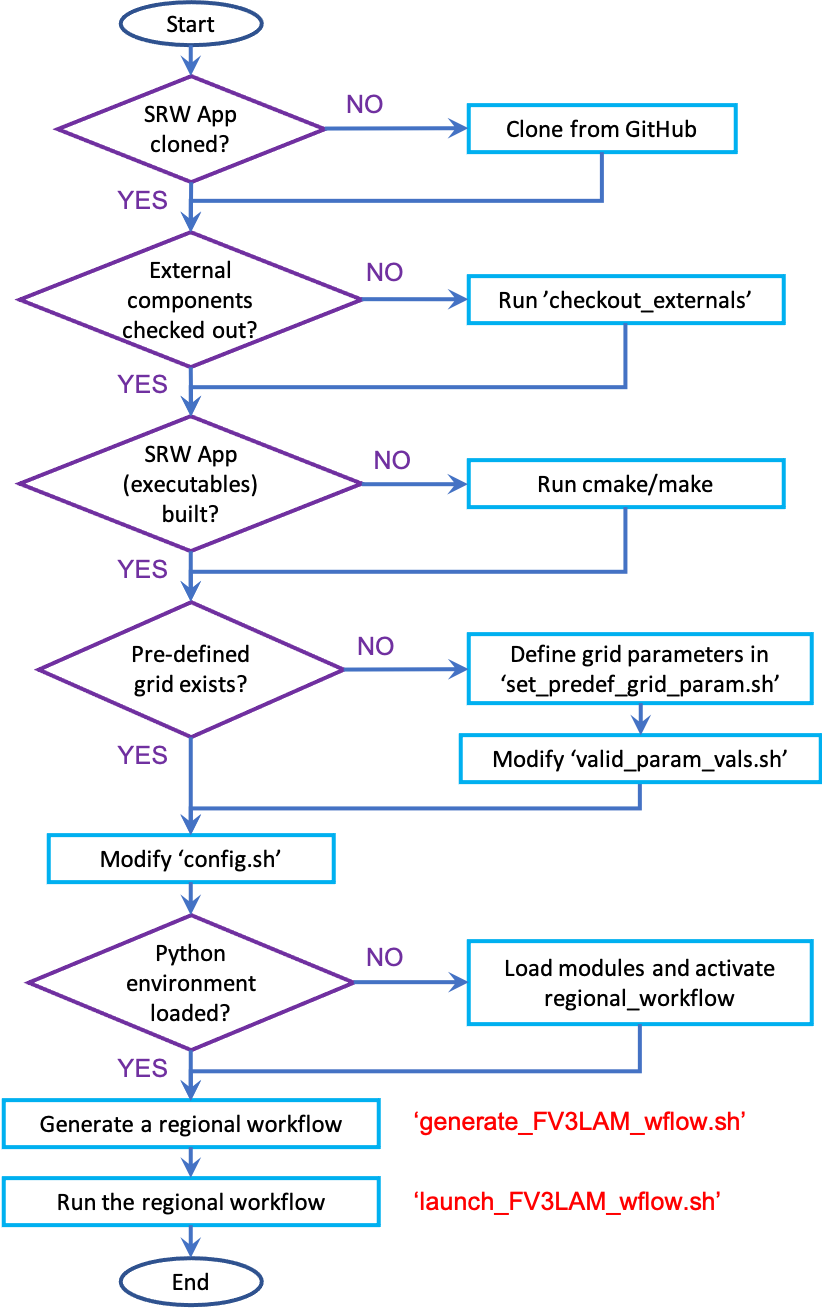
\includegraphics[width=0.6\linewidth]{FV3LAM_wflow_overall.png}
  \caption{Overall procedure of Short Range Weather App}
  \label{fig:srw_overall}
\end{figure}




%=================================================== 
\section{Download from GitHub}
\label{sec:pre_work_git}

Retrieve the `UFS Short Range Weather Application (SRWeather App)' repository from the specific GitHub repository to use the stable version of the regional workflow as follows:

\lstset{language=bash}   
\begin{lstlisting}[frame=trBL]
git clone -b master https://github.com/ufs-community/ufs-srweather-app
\end{lstlisting}

{\bf Note)} You should load the `git' module to clone a GitHub repository on WCOSS-Cray:
\lstset{language=bash}   
\begin{lstlisting}[frame=trBL]
module use -a /usrx/local/dev/modulefiles
module load git/2.18.0
\end{lstlisting}


The cloned repository contains the following sub-repositories and files:
{
\fontsize{10}{12}\selectfont
\begin{longtable}{ p{0.28\linewidth} | p{0.57\linewidth} }
\hline
\hline
 Directory/file name & Description \\
\hline
 docs & Release notes, documentation, users' guide  \\
 env & Machine-specific environment for set-up and workflow \\
 manage\_externals & Method for checking out external components\\
 src & Build scripts are initially located, and the external components will be cloned in this directory.  \\
\hdashline
 CMakeLists.txt & Main {\it cmake} file for UFS Short Range Weather Application \\
 Externals.cfg & GitHub repositories/branches for the external components \\
 LICENSE.md & (empty) \\
 README.md & Quick users' guide \\
 ufs\_srweather\_app\_meta.h.in & Meta information for UFS Short Range Weather Application which can be used by other packages  \\
 ufs\_srweather\_app.settings.in & UFS Short Range Weather App configuration summary \\
\hdashline
 regional\_workflow & Regional workflow (This directory will be created by running `checkout\_externals' in Section \ref{sec:pre_work_ext}). \\
 bin & Executables for workflow (This directory will be created by running `cmake/make' in Section \ref{sec:build_exec}.) \\
 include, lib, share & Modules, library, and input files for post-processing (This directory will be created by running `cmake/make' in Section \ref{sec:build_exec}.) \\
\hline
\caption{Sub-directories of the short range weather application}
\label{table:srwapp_dir}
\end{longtable}
}



%=================================================== 
\section{External Components}
\label{sec:pre_work_ext}

For the purpose of maintenance on WCOSS, the stable tag of the regional workflow for EMC utilizes the specific hash numbers for the external components as shown in Table \ref{table:stable_hash_ext} rather than branch names.
\lstset{language=bash}   
\begin{lstlisting}[frame=trBL]
cd {HOME}
vim Externals.cfg
(Update the hash numbers to the latest)
\end{lstlisting}

Check out the sub-modules such as regional\_workflow, ufs\_weather\_model, ufs\_utils, and emc\_post for UFS Short Range Weather Application:
\lstset{language=bash}   
\begin{lstlisting}[frame=trBL]
./manage_externals/checkout_externals
\end{lstlisting}
where `\{HOME\}' is the path to the `ufs-srweather-app' repository. For example, it can be `/scratch2/ NCEPDEV/fv3-cam/\{LOGNAME\}/ufs-srweather-app' on Hera. \\

{\bf Note)} 
\begin{itemize}
\item It should be run from the \{HOME\} directory where the `Externals.cfg' file exists to avoid the root error saying `Model description file does not exist at path'.
\item On WCOSS-Cray (Luna/Surge), you should load Python correctly:
\lstset{language=bash}   
\begin{lstlisting}[frame=trBL]
module load python/3.6.3.  (2.7.xx or higher should be loaded)
\end{lstlisting}
\end{itemize}

This step will use the configuration file `Externals.cfg' in the `\{HOME\}' directory to clone the specific branches (or hashes) of the external components as listed in Table \ref{table:ext_comp_github}. As a result, the regional workflow are cloned in the \{HOME\} directory while the external components are cloned into the target sub-directories in the `\{HOME\}/src' directory as shown in Figure \ref{figure:srwapp_dir}. The directories and sub-directories that will be created later by running the scripts are presented in parentheses. 

\begin{figure}[ht!]
\centering
\begin{minipage}{0.65\linewidth}
\dirtree{%
.1 ufs-srweather-app.
.2 (bin / build / include / lib / share).
.2 docs.
.2 env.
.2 manage\_externals.
.2 {\bf regional\_workflow}.
.3 docs.
.3 jobs.
.3 modulefiles.
.3 scripts.
.3 tests.
.4 baseline\_configs.
.3 ush.
.4 bash\_utils.
.4 Python.
.4 rocoto.
.4 templates.
.5 parm.
.6 met.
.6 metplus.
.4 wrappers.
.2 src.
.3 EMC\_post.
.4 parm.
.4 sorc.
.5 ncep\_post.fd.
.3 UFS\_UTILS.
.4 sorc.
.5 chgres\_cube.fd.
.5 grid\_tools.fd.
.5 orog\_mask\_tools.fd.
.4 ush.
.3 ufs\_weather\_model.
.4 FV3.
.5 atmos\_cubed\_sphere.
.5 ccpp.
.5 tests.
}
\end{minipage}
\caption{Structure of UFS Short Range Weather App}
\label{figure:srwapp_dir}
\end{figure}

{
\fontsize{10}{12}\selectfont
\begin{longtable}{ p{0.2\linewidth} | p{0.35\linewidth}  | p{0.25\linewidth}  }
\hline
\hline
 Component & GitHub repository (branch) & Target sub-directory \\
\hline
 regional\_workflow & NOAA-EMC/regional\_workflow & regional\_workflow \\
 & (develop) & \\ 
\hdashline
 ufs\_utils & NOAA-EMC/UFS\_UTILS & src/UFS\_UTILS \\
  & (develop) & \\
 ufs\_weather\_model & ufs-community/ufs-weather-model & src/ufs\_weather\_model  \\
  & (develop) & \\
 EMC\_post & NOAA-EMC/EMC\_post & src/EMC\_post \\
  & (develop) & \\
\hline
\caption{GitHub repository for the external components}
\label{table:ext_comp_github}
\end{longtable}
}

{\bf Notes)}
\begin{itemize}
\item The target sub-directories are not shown in the \{HOME\} or `\{HOME\}/src' directory until the `checkout\_externals' is executed.
\item The source codes of the executables such as `chgres\_cube', 'global\_equiv\_resol', `orog', and `shave' are located in `\{HOME\}/src/UFS\_UTILS/sorc/' (`ufs\_utils' component).
\end{itemize}


\subsubsection{Workflow with Another Hash or HEAD}

If you want to run the workflow with another hash or with the latest version (HEAD) of a given repository/branch (e.g. stable version/tag of the regional workflow), you will have to modify the `Externals.cfg' file before issuing the above `./checkout\_externals' command. 

\begin{enumerate}
\item Check the current hash or HEAD of the external component in `Externals.cfg':
\lstset{language=bash}   
\begin{lstlisting}[frame=trBL]
[ufs_utils]
protocol = git
repo_url = https://github.com/NOAA-EMC/regional_workflow
# Specify either a branch name or a hash but not both.
#branch = develop
hash = 6891c8a
local_path = regional_workflow
required = True
\end{lstlisting}
Note that the `branch' property in the above block (for `regional\_workflow') is commented out (using the \# character), and instead the `hash' property is specified.

\item To have `manage\_externals' obtain a different hash, simply specify a different hash in the line `hash=6891c8a' in the block above. 

\item To obtain the HEAD of the `develop' branch, uncomment the line specifying the branch and comment out the line specifying the hash as follows:
\lstset{language=bash}   
\begin{lstlisting}[frame=trBL]
branch = develop
#hash = 6891c8a
\end{lstlisting}

\end{enumerate}


The regional workflow contains the sub-directories and files as shown in Table \ref{table:workflow_dir}:
\lstset{language=bash}   
\begin{lstlisting}[frame=trBL]
cd {HOMErrfs}
\end{lstlisting}
where `\{HOMErrfs\}' is the path to the `regional\_workflow' repository. For example, it can be `scratch2/NCEPDEV/fv3-cam/\{LOGNAME\}/ufs-srweather-app/regional\_workflow' on Hera.

{
\fontsize{10}{12}\selectfont
\begin{longtable}{ p{0.2\linewidth} | p{0.55\linewidth} }
\hline
\hline
 Directory/file name & Description \\
\hline
 docs & Release notes, documentation, users' guides  \\
 jobs & J-job scripts which are launched by {\it Rocoto} \\
 modulefiles & Module files required for running the model \\
 scripts & Run scripts launched by the J-jobs \\
 tests & Baseline experiment configurations \\
 ush & Utility scripts called by various run scripts\\
\hdashline
 environment.yml & \\
 README.md & Quick user's guide to run a FV3-LAM workflow \\
 update\_fork.pl & \\
\hline
\caption{Initial sub-directories and files of the regional workflow}
\label{table:workflow_dir}
\end{longtable}
}




%=================================================== 
\section{Building the Executables for Workflow}
\label{sec:build_exes_wflow}

%---------------------------------------------------------
\subsection{Environment Set-up}
\label{sec:build_env}

Load the required modules and set the environment variables for `BASH' users in the `build\_env\_ [machine]\_[compiler].sh' file as:
\lstset{language=bash}   
\begin{lstlisting}[frame=trBL]
cd {HOME}/env/
source build_[machine]_[compiler].env
module list
\end{lstlisting}
where `[machine]' is `hera', `wcoss\_dell\_p3', `wcoss\_cray', or `orion', and `[compiler]' is `intel'.

\vspace{0.5cm}


{\bf Notes)} 
\begin{itemize}
\item The above file (`build\_[machine]\_[compiler].env') is sourced from the script `\{HOMErrfs\}/ush/load\_modules\_run\_task.sh' when a task is launched. Therefore, if you want to change the file name and its path, you should modify the script (lines 156--157):
\lstset{language=bash}   
\begin{lstlisting}[frame=trBL]
155 machine=${MACHINE,,}
156 env_fn="build_${machine}_${COMPILER}.env"
157 env_fp="${SR_WX_APP_TOP_DIR}/env/${env_fn}"
\end{lstlisting}

\item If you use `TCSH' on Hera, you should change the environment variables in the last four lines as follows:
\lstset{language=bash}   
\begin{lstlisting}[frame=trBL]
setenv CMAKE_C_COMPILER mpiicc
setenv CMAKE_CXX_COMPILER mpiicpc
setenv CMAKE_Fortran_COMPILER mpiifort
setenv CMAKE_Platform hera.intel
\end{lstlisting}
\end{itemize}



%---------------------------------------------------------
\subsection{Building the Executables}
\label{sec:build_exec}


Build a regional workflow system including the preprocessing utilities, forecast model, and post-processor:
\lstset{language=bash}   
\begin{lstlisting}[frame=trBL]
cd {HOME}
mkdir build
cd build

cmake .. -DCMAKE_INSTALL_PREFIX=..
make -j 8 >& build.out &
\end{lstlisting}
where `-DCMAKE\_INSTALL\_PREFIX' specifies the location where the bin, include, lib, and share directories containing various components of SRW App will be created, and its recommended value `..' denotes one directory up from the build directory. In the next line for the {\it make} call,  `-j 8' means the parallel run with 8 threads. \\

When the build process completes, there should exist  the forecast model executable `ufs\_model' and eleven pre- and post-processing executables in `\{HOME\}/bin/', as shown in Table \ref{table:list_exe}:
{
\fontsize{10}{12}\selectfont
\begin{longtable}{ p{0.18\linewidth} | p{0.56\linewidth} | p{0.14\linewidth} }
\hline
\hline
 Name & Description  & Detail \\
\hline
 chgres\_cube & Creates IC/LBC & Section \ref{sec:glb2reg_chgrescube} \\
 filter\_topo & Filters the orography & Section \ref{sec:sar_pre_filttopo} \\
 global\_equiv\_resol & Computes the global equivalent resolution for ESG grids & Section \ref{subsec:global_eqv_res} \\
 make\_hgrid & Creates the grid files which contain geo-referencing records for the model grid including global uniform and GFDL stand-alone regional grids & Section \ref{sec:sar_pre_grid}\\
 make\_solo\_mosaic & Creates the mosaic files & Sections \ref{subsec:mosaic_halo} \& \ref{sec:sar_pre_grid} \\
 ncep\_post & Post-processing & Section \ref{sec:post_grb2} \\
 ufs\_model & UFS weather model executable & Chapter \ref{chpt:ufs_weather_model} \\
 orog & Computes land mask, orography and gravity wave drag  & Section \ref{sec:sar_pre_orog} \\
 regional\_esg\_grid &Creates the stand-alone ESG grid files & Section \ref{subsec:new_predef_grid_esg} \\
 sfc\_climo\_gen & Creates surface climatological fields such as soil type & Sections \ref{sec:sar_wflow_static} \& \ref{sec:sar_pre_fix} \\
 shave & Shaves the excess halo rows down to what is required for the LBCs in the orography and grid files & Section \ref{sec:sar_pre_halo} \\
 vcoord\_gen & Generate hybrid coordinate interface profiles & - \\
\hline
\hline
\caption{List of executables.}
\label{table:list_exe}
\end{longtable}
}


%---------------------------------------------------------
\subsection{Adding a New CCPP Suite to SRW App}
\label{sec:add_ccpp}

To add a new CCPP Suite to the SRW App, you should modify/add some files {\bf before} building the app described in Section \ref{sec:build_exec}:

\begin{enumerate}
\item Add the name of a new CCPP suite to the list in `\{HOME\}/src/CMakeLists.txt':
\lstset{language=bash}   
\begin{lstlisting}[frame=trBL,basicstyle=\scriptsize]
if(NOT CCPP_SUITES)
  set(CCPP_SUITES "FV3_CPT_v0,FV3_GFS_2017_gfdlmp,FV3_GFS_2017_gfdlmp_regional,FV3_GSD_SAR,FV3_GSD_v0,FV3_GFS_v15p2,FV3_GFS_v16beta,FV3_RRFS_v1beta,FV3_HRRR,RRFS_parallel")
endif()
\end{lstlisting}

\item Add a new `suite\_[new CCPP suite].xml' file to `\{HOME\}/src/ufs\_weather\_model/FV3/ccpp/ suites'.

\item Add the name of a new CCPP suite to the list in `\{HOMErrfs\}/ush/valid\_param\_vals.sh':
\lstset{language=bash}   
\begin{lstlisting}[frame=trBL,basicstyle=\scriptsize]
valid_vals_CCPP_PHYS_SUITE=( \
"FV3_CPT_v0" \
"FV3_GFS_2017_gfdlmp" \
"FV3_GFS_2017_gfdlmp_regional" \
"FV3_GSD_SAR" \
"FV3_GSD_v0" \
"FV3_GFS_v15p2" \
"FV3_GFS_v16beta" \
"FV3_RRFS_v1beta" \
"FV3_RRFS_v1alpha" \
"FV3_HRRR" \
"RRFS_parallel" \
)
\end{lstlisting}

\item Add/modify the template files for a new CCPP suite to `\{HOMErrfs\}/ush/templates':
\begin{itemize}
\item diag\_table.[new CCPP suite]
\item field\_table.[new CCPP suite]
\item FV3.input.yml
\end{itemize}

\item Modify `varmap\_file' in `\{HOMErrfs\}/scripts/exregeional\_make\_ics.sh':
\lstset{language=bash}   
\begin{lstlisting}[frame=trBL,basicstyle=\scriptsize]
case "${CCPP_PHYS_SUITE}" in
#
  "FV3_GFS_2017_gfdlmp" | \
  "FV3_GFS_2017_gfdlmp_regional" | \
  "FV3_GFS_v16beta" | \
  "FV3_GFS_v15p2" | "FV3_CPT_v0" )
    varmap_file="GFSphys_var_map.txt"
    ;;
#
  "FV3_GSD_v0" | \
  "FV3_GSD_SAR" | \
  "RRFS_parallel" | \
  "FV3_RRFS_v1alpha" | \
  "FV3_RRFS_v1beta" | \
  "FV3_HRRR" )
    if [ "${EXTRN_MDL_NAME_ICS}" = "RAP" ] || \
       [ "${EXTRN_MDL_NAME_ICS}" = "HRRR" ]; then
      varmap_file="GSDphys_var_map.txt"
    elif [ "${EXTRN_MDL_NAME_ICS}" = "NAM" ] || \
         [ "${EXTRN_MDL_NAME_ICS}" = "FV3GFS" ] || \
         [ "${EXTRN_MDL_NAME_ICS}" = "GSMGFS" ]; then
      varmap_file="GFSphys_var_map.txt"
    fi
    ;;
\end{lstlisting}

\item Modify `varmap\_file' in `\{HOMErrfs\}/scripts/exregeional\_make\_lbcs.sh':
\lstset{language=bash}   
\begin{lstlisting}[frame=trBL,basicstyle=\scriptsize]
case "${CCPP_PHYS_SUITE}" in
#
  "FV3_GFS_2017_gfdlmp" | \
  "FV3_GFS_2017_gfdlmp_regional" | \
  "FV3_GFS_v16beta" | \
  "FV3_GFS_v15p2" | "FV3_CPT_v0" )
    varmap_file="GFSphys_var_map.txt"
    ;;
#
  "FV3_GSD_v0" | \
  "FV3_GSD_SAR" | \
  "RRFS_parallel" | \
  "FV3_RRFS_v1alpha" | \
  "FV3_RRFS_v1beta" | \
  "FV3_HRRR" )
    if [ "${EXTRN_MDL_NAME_LBCS}" = "RAP" ] || \
       [ "${EXTRN_MDL_NAME_LBCS}" = "HRRR" ]; then
      varmap_file="GSDphys_var_map.txt"
    elif [ "${EXTRN_MDL_NAME_LBCS}" = "NAM" ] || \
         [ "${EXTRN_MDL_NAME_LBCS}" = "FV3GFS" ] || \
         [ "${EXTRN_MDL_NAME_LBCS}" = "GSMGFS" ]; then
      varmap_file="GFSphys_var_map.txt"
    fi
    ;;
\end{lstlisting}


\end{enumerate}



%=================================================== 
\section{Generating a Regional Workflow Experiment}
\label{sec:workflow_newreg}

%---------------------------------------------------------
\subsection{Steps to Generate a New Regional Workflow Experiment}
\label{subsec:wflow_flowchart}

{\bf First}, check if a pre-defined grid exists in the grid-specific configuration file (see the detail in Sections \ref{subsec:wflow_predef_grid_parm} and \ref{subsec:wflow_valid_val}):
\lstset{language=bash}   
\begin{lstlisting}[frame=trBL]
cd {HOMErrfs}/ush
vim set_predef_grid_param.sh
vim valid_param_vals.sh
\end{lstlisting}

\vspace{0.5cm}

{\bf Second}, create a user-specified experiment configuration file (`\{HOMErrfs\}/ush/config.sh') and specify the values of your experiment parameters in it (see the detail in Sections \ref{subsec:wflow_config_default} and \ref{subsec:wflow_config_new}):
\lstset{language=bash}   
\begin{lstlisting}[frame=trBL]
cd {HOMErrfs}/ush
cp config.[option].sh config.sh
vim config.sh
# Edit parameters as needed.
\end{lstlisting}
where `config.[option].sh' is described in Section \ref{subsec:wflow_config_new}. For users’ convenience, two example configuration files are provided in `\{HOMErrfs\}/ush/': `config.community.sh' and `config.nco.sh'. The first is an example for creating and running an experiment in the `community' mode (i.e. with the parameter `RUN\_ENVIR' set to ``community''), while the second is an example of creating and running an experiment in the `NCO' (operational) mode (i.e. with `RUN\_ENVIR' set to ``nco''). \\

{\bf Third}, check templates of the input files and modify them as needed (Section \ref{sec:workflow_template}). \\

{\bf Fourth}, modify the `set\_cycle\_dates.sh' script if you want to change the frequency of cycles. The frequency is set to one day in the script, and it is not able to be adjusted in the `config.sh' file.
\lstset{language=bash}   
\begin{lstlisting}[frame=trBL]
cd {HOMErrfs}/ush
vim set_cycle_dates.sh
\end{lstlisting}
 
Change the number of `\# days' (default: 1) on Line 109 as follows:
\lstset{language=bash}   
\begin{lstlisting}[frame=trBL, basicstyle=\scriptsize]
105   all_cdates=()
106   date_crnt="${date_start}"
107   while [ "${date_crnt}" -le "${date_end}" ]; do
108     all_cdates+=( $( printf "%s " ${cycle_hrs[@]/#/${date_crnt}} ) )
109     date_crnt=$( date -d "${date_crnt} + 1 days" +%Y%m%d )
110   done
\end{lstlisting}
  
 
 \vspace{0.5cm}

{\bf Fifth}, check additional steps only for the `{\bf nco}' mode:

\begin{enumerate}
\item Check if the FIX files necessary for running the `nco' mode exist in the designated directory, which is specified in `config.sh', as described in Section \ref{subsec:wflow_fix_nco}.

\item Create mosaic halo files (`mosaic.halo[3,4,6].nc'):

If the mosaic halo files named `mosaic.halo[3,4,6].nc' do not exist in the above designated directory, you should create them as described in Section \ref{subsec:mosaic_halo}.

\end{enumerate}

 \vspace{0.5cm}

{\bf Sixth}, load the appropriate {\it Python} environment for the workflow. The workflow requires {\it Python3} with the packages `PyYAML', `Jinja2', and `f90nml' available.
\lstset{language=bash}   
\begin{lstlisting}[frame=trBL]
cd {HOME}/env/
source wflow_[machine].env
\end{lstlisting}

This file includes machine-specific {\it Python} environment as follows:
\begin{itemize}
\item On Hera:
\lstset{language=bash}   
\begin{lstlisting}[frame=trBL]
module use -a /contrib/miniconda3/modulefiles
module load miniconda3
conda activate regional_workflow
\end{lstlisting}

\item On WCOSS\_dell\_p3 (Mars/Venus):
\lstset{language=bash}   
\begin{lstlisting}[frame=trBL]
module load python/3.6.3
module use /usrx/local/nceplibs/dev/modulefiles
module load srw-app-python/1.0.0
\end{lstlisting}

\item On WCOSS\_cray (Luna/Surge):
\lstset{language=bash}   
\begin{lstlisting}[frame=trBL]
module unload python/2.7.14
module load python/3.6.3
module use /usrx/local/nceplibs/modulefiles
module load srw-app-python/1.0.0
\end{lstlisting}

\item On Orion:
\lstset{language=bash}   
\begin{lstlisting}[frame=trBL]
module use -a /apps/contrib/miniconda3-noaa-gsl/modulefiles
module load miniconda3
conda activate regional_workflow
\end{lstlisting}

\end{itemize}


\vspace{0.5cm}

{\bf Seventh}, generate the workflow:
\lstset{language=bash}   
\begin{lstlisting}[frame=trBL]
cd {HOMErrfs}/ush
./generate_FV3LAM_wflow.sh
\end{lstlisting}

\vspace{0.5cm}

The flowchart for generating a new regional workflow is shown in Figure \ref{fig:workflow_gen}.

\begin{figure}[ht!]
  \centering
  \includegraphics[width=0.8\linewidth]{Fv3regional_workflow_gen.png}
  \caption{Structure of workflow generation}
  \label{fig:workflow_gen}
\end{figure}

\begin{itemize}
\item The default configuration file (`\{HOMErrfs\}/ush/config\_default.sh') assigns default values to the experiment parameters.  Some of these default values are intentionally invalid in order to force the user to assign them valid values in the user-specified configuration file.  There is usually no need for a user to modify the default configuration file.  Note that the default configuration file also contains documentation describing the experiment parameters.

\item Parameter settings in the user-specified configuration file (`\{HOMErrfs\}/ush/config.sh') will override settings in the default configuration file because the user-specified configuration file is sourced after the default one.

\item As shown in the flowchart, the grid(domain)-specific parameters such as the GFDL grid refinement or ESG (JP) grid, write-component parameters when `QUILTING'=``TRUE'', `DT\_ATMOS', `LAYOUT\_X(Y)', and `BLOCKSIZE', are separately set in `\{HOMErrfs\} /ush/set\_predef\_grid\_params.sh'. If you want to use other regional domains that are not defined in this file, you should modify this file.

\end{itemize}


%---------------------------------------------------------
\subsection{Pre-defined Grid Parameters: `set\_predef\_grid\_params.sh'}
\label{subsec:wflow_predef_grid_parm}

This file defines grid parameters for the specific pre-defined grids. The list of the pre-defined grids can be found in Table \ref{table:config_validval} (`PREDEF\_GRID\_NAME'). The grid parameters, defined in this file, are as follows:

\begin{enumerate}
\item Pre-defined grids:
{
\fontsize{10}{12}\selectfont
\begin{longtable}{p{0.03\linewidth} | p{0.26\linewidth} | p{0.35\linewidth} | p{0.2\linewidth}   }
\hline
\hline
No. & Grid name & Description  & Method(s) \\
\hline
1 & RRFS\_CONUS\_25km & GSD's 25$km$ CONUS domain & ESGgrid \\
2 & RRFS\_CONUS\_13km & GSD's 13$km$ CONUS domain & ESGgrid \\
3 & RRFS\_CONUS\_3km & GSD's 3$km$ CONUS domain & ESGgrid \\
4 & RRFS\_SUBCONUS\_3km & GSD's 3$km$ sub-CONUS domain & ESGgrid \\
5 & RRFS\_AK\_13km & GSD's 13$km$ HRRR Alaska grid & ESGgrid \\
6 & RRFS\_AK\_3km & GSD's 3$km$ HRRR Alaska grid & ESGgrid \\
7 & CONUS\_25km\_GFDLgrid & GFDL 25$km$ CONUS domain & GFDLgrid \\
8 & CONUS\_3km\_GFDLgrid & GFDL 3$km$ CONUS domain & GFDLgrid \\
9 & EMC\_AK & EMC's 3$km$ Alaska grid & ESGgrid \\
10 & EMC\_HI & EMC's 3$km$ Hawaii grid & ESGgrid \\
11 & EMC\_PR & EMC's 3$km$ Puerto Rico grid & ESGgrid \\
12 & EMC\_GU & EMC's 3$km$ Guam grid & ESGgrid \\
13 & GSL\_HAFSV0.A\_25km & HAFS v0.A grid at 25$km$ & ESGgrid \\
14 & GSL\_HAFSV0.A\_13km & HAFS v0.A grid at 13$km$ & ESGgrid \\
15 & GSL\_HAFSV0.A\_3km & HAFS v0.A grid at 3$km$ &  ESGgrid \\
16 & GSD\_HRRR\_AK\_50km & GSD's 50$km$ HRRR Alaska grid & ESGgrid \\
17 & GSD\_RAP13km & GSD's RAP grid & ESGgrid \\
\hline
\caption{Pre-defined grids}
\label{table:predefined_grids}
\end{longtable}
}

\item Parameters for the GFDL grid refinement (Table \ref{table:config_GFDLgrid}) or ESG grid (Table \ref{table:config_JPgrid}).
\item Parameters for configurations in `input.nml' and `model\_configuration' (Table \ref{table:config_configparam}).
\item Parameters for the write components in case of `QUILTING'=``TRUE'':
\begin{enumerate}
\item `regional\_latlon' or `rotated\_latlon':
{
\fontsize{10}{12}\selectfont
\begin{longtable}{ p{0.26\linewidth} | p{0.65\linewidth}   }
\hline
\hline
 Parameter name & Description (Unit: in degrees)\\
\hline
 WRTCMP\_cen\_lon & Central longitude of the output domain \\
 WRTCMP\_cen\_lat & Central latitude of the output domain \\
 WRTCMP\_lon\_lwr\_left & Longitudinal distance from the center to the bottom-left corner \\
 WRTCMP\_lat\_lwr\_left & Latitudinal distance from the center to the bottom-left corner \\
 WRTCMP\_lon\_upr\_rght & Longitudinal distance from the center to the top-right corner \\
 WRTCMP\_lat\_upr\_rght & Latitudinal distance from the center to the top-right corner \\
 WRTCMP\_dlon & Longitudinal distance between two adjacent output-grid points \\
 WRTCMP\_dlat & Latitudinal distance between two adjacent output-grid points \\
\hline
\caption{Parameters for `regional\_latlon' or `rotated\_latlon'}
\label{table:gridpara_rotated}
\end{longtable}
}

\item `lambert\_conformal':
{
\fontsize{10}{12}\selectfont
\begin{longtable}{ p{0.26\linewidth} | p{0.65\linewidth}   }
\hline
\hline
 Parameter name & Description  \\
\hline
 WRTCMP\_cen\_lon & Central longitude of the output domain (in degrees)  \\
 WRTCMP\_cen\_lat & Central latitude of the output domain (in degrees) \\
 WRTCMP\_stdlat1 & Latitude of the first standard parallel (in degrees) \\
 WRTCMP\_stdlat2 & Latitude of the second standard parallel (in degrees) \\
 WRTCMP\_nx & Total number of grid points along $x$-axis \\
 WRTCMP\_ny & Total number of grid points along $y$-axis  \\
 WRTCMP\_lon\_lwr\_left & Longitude of the bottom-left corner of output (in degrees) \\
 WRTCMP\_lat\_lwr\_left & Latitude of the bottom-left corner of output (in degrees) \\
 WRTCMP\_dx & Grid cell size in $x$ direction (in meters) \\
 WRTCMP\_dy & Grid cell size in $y$ direction (in meters) \\
\hline
\caption{Parameters for `lambert\_conformal'}
\label{table:gridpara_lambert}
\end{longtable}
}

{\bf Notes)} As shown in Figure \ref{fig:workflow_gen}, The script `set\_predef\_grid\_params.sh' is issued later than `config.sh'. Therefore, if any parameters are set in both scripts, the parameters in `set\_predef\_grid\_params.sh' will be finally used in the model.

\end{enumerate}

\end{enumerate}



%---------------------------------------------------------
\subsection{Valid Values for Configuration Parameters: `valid\_param\_vals.sh'}
\label{subsec:wflow_valid_val}

The valid values for the experiment's configuration parameters:
{
%\fontsize{10}{12}\selectfont
\scriptsize
\begin{longtable}{p{0.02\linewidth} | p{0.3\linewidth} | p{0.6\linewidth} }
\hline
\hline
 & Parameter name & Valid values   \\
\hline
1 & RUN\_ENVIR & ``nco'', ``community'' \\
2 & VERBOSE & ``TRUE'', ``YES'', ``FALSE'', ``NO''\\
3 & MACHINE & ``WCOSS\_CRAY'', ``WCOSS\_DELL\_P3'', ``HERA'', ``ORION'', ``JET'', ``ODIN'', ``CHEYENNE'', ``STAMPEDE'' \\
4 & SCHED & ``slurm'', ``pbspro'', ``lsf'', ``lsfcray'', ``none'' \\
5 & PREDEF\_GRID\_NAME & ``RRFS\_CONUS\_25km'', ``RRFS\_CONUS\_13km'', ``RRFS\_CONUS\_3km'', ``RRFS\_SUBCONUS\_3km'', ``RRFS\_AK\_13km'', ``RRFS\_AK\_3km, ``CONUS\_25km\_GFDLgrid'', ``CONUS\_3km\_GFDLgrid'', ``EMC\_AK'', ``EMC\_HI'', ``EMC\_PR'', ``EMC\_GU'', ``GSL\_HAFSV0.A\_25km'', ``GSL\_ HAFSV0.A\_13km'', ``GSL\_HAFSV0.A\_3km'',  ``GSD\_HRRR\_AK\_50km'', ``GSD\_RAP13km''  \\
6 & CCPP\_PHYS\_SUITE & ``FV3\_CPT\_v0'', ``FV3\_GFS\_2017\_gfdlmp\_regional'', ``FV3\_GSD\_SAR'', ``FV3\_GSD\_v0'', ``FV3\_GFS\_v15p2'', ``FV3\_GFS\_v16beta'', ``FV3\_RRFS\_ v1beta'', ``FV3\_RRFS\_v1alpha'', ``FV3\_HRRR'' \\
7 & GFDLgrid\_RES & ``48'', ``96'', ``192'', ``384'', ``768'', ``1152'', ``3072'' \\
8 & EXTRN\_MDL\_NAME\_ICS & ``GSMGFS'', ``FV3GFS'', ``RAP'', ``HRRR'', ``NAM'' \\
9 & EXTRN\_MDL\_NAME\_LBCS & ``GSMGFS'', ``FV3GFS'', ``RAP'', ``HRRR'', ``NAM'' \\
10 & FV3GFS\_FILE\_FMT\_ICS & ``nemsio'', ``grib2'', ``netcdf'' \\
11 & FV3GFS\_FILE\_FMT\_LBCS & ``nemsio'', ``grib2'', ``netcdf'' \\
12 & GIRD\_GEN\_METHOD & ``GFDLgrid'', ``ESGgrid''\\
13 & PREEXISTING\_DIR\_ METHOD & ``delete'', ``rename'', ``quit'' \\
14 & GTYPE & ``regional'' \\
15 & WRTCMP\_output\_grid & ``rotated\_latlon'', ``lambert\_conformal'', ``regional\_latlon'' \\
16 & RUN\_TASK\_MAKE\_GRID & ``TRUE'', ``YES'', ``FALSE'', ``NO'' \\
17 & RUN\_TASK\_MAKE\_OROG & ``TRUE'', ``YES'', ``FALSE'', ``NO'' \\
18 & RUN\_TASK\_MAKE\_SFC\_ CLIMO & ``TRUE'', ``YES'', ``FALSE'', ``NO'' \\
19 & RUN\_TASK\_VX\_GRIDSTAT & ``TRUE'', ``YES'', ``FALSE'', ``NO'' \\
20 & RUN\_TASK\_VX\_POINTSTAT & ``TRUE'', ``YES'', ``FALSE'', ``NO'' \\
21 & QUILTING & ``TRUE'', ``YES'', ``FALSE'', ``NO'' \\
22 & PRINT\_ESMF & ``TRUE'', ``YES'', ``FALSE'', ``NO'' \\
23 & USE\_CRON\_TO\_RELAUNCH & ``TRUE'', ``YES'', ``FALSE'', ``NO'' \\
24 & DOT\_OR\_USCORE & ``.'', ``\_'' \\
25 & NOMADS & ``TRUE'', ``YES'', ``FALSE'', ``NO'' \\
26 & NOMADS\_file\_type & ``TRUE'', ``YES'', ``FALSE'', ``NO'' \\
27 & DO\_ESEMBLE & ``TRUE'', ``YES'', ``FALSE'', ``NO'' \\
28 & USE\_CUSTOM\_POST\_CONFIG\_FILE & ``TRUE'', ``YES'', ``FALSE'', ``NO'' \\
29 & DO\_SHUM & ``TRUE'', ``YES'', ``FALSE'', ``NO'' \\
30 & DO\_SPPT & ``TRUE'', ``YES'', ``FALSE'', ``NO'' \\
31 & DO\_SKEB & ``TRUE'', ``YES'', ``FALSE'', ``NO'' \\
32 & USE\_ZMTNBLCK & ``TRUE'', ``YES'', ``FALSE'', ``NO'' \\
33 & USE\_FVCOM & ``TRUE'', ``YES'', ``FALSE'', ``NO'' \\
34 & COMPILER & ``intel'', ``gnu'' \\
\hline
\caption{Valid values for the configuration parameters}
\label{table:config_validval}
\end{longtable}
}



%---------------------------------------------------------
\subsection{CCPP Suites Supported in FV3-LAM}
\label{subsec:ccpp_suites_kinds}

{\bf References)} 
\begin{itemize}
\item \url{https://ccpp-techdoc.readthedocs.io/en/latest/Overview.html} 
\item \url{https://dtcenter.ucar.edu/GMTB/v4.0/sci_doc/index.html}
\end{itemize}

The Common Community Physics Package (CCPP) is composed of two parts: infrastructure (CCPP-Framework) and library of physical parameterizations (CCPP-Physics). The suites that are supported for FV3-LAM can be found in Table \ref{table:config_validval} (No.6; under `CCPP\_PHYS\_SUITE'). The types of parameterization for each suite are listed in Table \ref{table:ccpp_suite_param}.

{
\fontsize{9}{11}\selectfont
\begin{longtable}{ p{0.16\linewidth} | p{0.35\linewidth} | p{0.35\linewidth}  }
\hline
\hline
\multirow{2}{*}{Parameterization} & \multicolumn{2}{c}{CCPP Suite}  \\ 
\cline{2-3}
 & GFS\_v15p2 & GFS\_v16beta  \\
\hline
Microphysics & GFDL Cloud Microphysics Scheme & GFDL Cloud Microphysics Scheme   \\
PBL & GFS Hybrid Eddy-Diffusivity Mass-Flux (K-EDMF) & GFS Scale-aware TKE-based Moist Eddy-Diffusion Mass-Flux (TKE-EDMF)  \\
Turbulence & Free Atmospheric Turbulence Scheme & Free Atmospheric Turbulence Scheme \\
Deep convection & GFS Scale-aware Simplified Arakawa-Schubert (sa-SAS) & GFS Scale-aware Simplified Arakawa-Schubert (sa-SAS)  \\
Shallow convection & GFS SAS-based Mass-Flux (sa-MF) & GFS SAS-based Mass-Flux (sa-MF)  \\
Radiation & Rapid Radiative Transfer Model for GCMs (RRTMG) & Rapid Radiative Transfer Model for GCMs (RRTMG)  \\
Surface layer & GFS Surface Layer Scheme & GFS Surface Layer Scheme  \\
Gravity wave drag & Unified Gravity Wave Drag (uGWD) & Unified Gravity Wave Drag (uGWD)  \\
Land surface & GFS Noah Land Surface Model & GFS Noah Land Surface Model  \\
Ozone & 2015 Navy Research Laboratory ozone and stratospheric water vapor schemes (NRL 2015) & 2015 Navy Research Laboratory ozone and stratospheric water vapor schemes (NRL 2015)   \\
H$_2$O & NRL 2015 & NRL 2015  \\
Ocean & Near-Surface Sea Temperature (NSST) & Near-Surface Sea Temperature (NSST)  \\
\hdashline
 & Operational & Experimental  \\
\hline
\caption{CCPP Suites: type of parameterization}
\label{table:ccpp_suite_param}
\end{longtable}
}




%---------------------------------------------------------
\subsection{Default Configuration: `config\_default.sh'}
\label{subsec:wflow_config_default}

This file sets the experiment's configuration parameters (global shell variables) to their default values. For many of these parameters, the valid values are defined in `\{HOMErrfs\}/ush/valid\_param\_vals.sh' (or Section \ref{subsec:wflow_valid_val}). Since this file contains the default settings, you do {\bf NOT} need to change it. The user-specified experimental parameters will be replaced by running the user-specified experimental configuration file `config.[option].sh'.

\begin{enumerate}
\item Experimental mode:
{
%\fontsize{10}{12}\selectfont
\scriptsize
\begin{longtable}{ p{0.2\linewidth} | p{0.5\linewidth} }
\hline
\hline
Parameter name & Description \\
\hline
RUN\_ENVIR & ``community'': community mode, or ``nco'': NCO mode \\
\hline
\caption{Configuration - experimental mode}
\label{table:config_expmode}
\end{longtable}
}

\item Machine and queue parameters:
{
%\fontsize{10}{12}\selectfont
\scriptsize
\begin{longtable}{ p{0.2\linewidth} | p{0.75\linewidth} }
\hline
\hline
Parameter name & Description \\
\hline
MACHINE & HPC machine on which the workflow runs \\
ACCOUNT & Account name to submit jobs to the queue on HPC  \\
SCHED & Job scheduler (e.g. `slurm') \\
PARTITION\_DEFAULT & Partition to which it will be submitted. If this is not set or is set to an empty string, it will be set to a machine-dependent value. This is not used if SCHED is not set to ``slurm''.\\
QUEUE\_DEFAULT & Default queue to which workflow tasks are submitted \\
PARTITION\_HPSS & Partition for the tasks that create links to external model files for IC and LBC.  If this is not set or is set to an empty string, it will be set to a machine-dependent value. This is not used if SCHED is not set to ``slurm''. \\
QUEUE\_HPSS & Queue for the external model files such as IC and LBC \\
PARTITION\_FCST & Partition for the task that runs forecasts. If this is not set or set to an empty string, it will be set to a machine-dependent value. This is not used if SCHED is not set to ``slurm''. \\
QUEUE\_FCST & Queue for a forecast run \\
\hline
\caption{Configuration - machine and queue}
\label{table:config_queue}
\end{longtable}
}

\item Cron-associated parameters:
{
%\fontsize{10}{12}\selectfont
\scriptsize
\begin{longtable}{p{0.3\linewidth} | p{0.6\linewidth} }
\hline
\hline
Parameter name & Description \\
\hline
USE\_CRON\_TO\_RELAUNCH & Flag to add a line to the user's cron table to call the experiment launch script every `CRON\_RELAUNCH\_ INTVL\_MNTS' minutes \\
CRON\_RELAUNCH\_INTVL\_MNTS & Interval (in minutes) between successive calls of the experiment launch script by a cron job \\
\hline
\caption{Configuration - cron}
\label{table:config_cron}
\end{longtable}
}

\item Experiment directories:
{
%\fontsize{10}{12}\selectfont
\scriptsize
\begin{longtable}{p{0.2\linewidth} | p{0.6\linewidth} }
\hline
\hline
Parameter name & Description \\
\hline
EXPT\_BASEDIR & Path and name of the base directory where the experiment is created  \\
EXPT\_SUBDIR & Name of the subdirectory in the base directory \\
\hline
\caption{Configuration - Experiment directories }
\label{table:config_expdir}
\end{longtable}
}

\item Parameters only for the NCO mode (when RUN\_ENVIR=``nco''):
{
%\fontsize{10}{12}\selectfont
\scriptsize
\begin{longtable}{p{0.22\linewidth} | p{0.68\linewidth} }
\hline
\hline
Parameter name & Description \\
\hline
COMINgfs & Path to the parent directory of the GFS input files for IC/LBC \\
FIXLAM\_NCO\_BASEDIR & Base directory containing pre-generated grid, orography, and surface climatology files \\
STMP & Path to the parent directory cycle-dependent model input files, symlinks to cycle-independent input files, and raw forecast output files\\
NET & Model name (first level of com directory structure) \\
envir & ``test'' for initial testing phase, ``para'' for run in parallel, ``prod'' in production \\
RUN & Name of model run (third level of com directory structure) \\
PTMP & Path to the parent directory of post-processed output files \\
\hline
\caption{Configuration - NCO mode}
\label{table:config_nco}
\end{longtable}
}

\item Separator character:
{
%\fontsize{10}{12}\selectfont
\scriptsize
\begin{longtable}{p{0.2\linewidth} | p{0.7\linewidth} }
\hline
\hline
Parameter name & Description \\
\hline
DOT\_OR\_USCORE & Separator (character) used for the names of the gird, mosaic, and orography fixed files \\
\hline
\caption{Configuration - Separator }
\label{table:config_separator}
\end{longtable}
}

\item File names:
{
%\fontsize{10}{12}\selectfont
\scriptsize
\begin{longtable}{p{0.2\linewidth} | p{0.56\linewidth} | p{0.16\linewidth} }
\hline
\hline
Parameter name & Description  & Default value \\
\hline
EXPT\_CONFIG\_FN & Name of the user-specified configuration file & config.sh \\
RGNL\_GRID\_NML\_FN & Name of the file containing the namelist settings for the ESG (JP) grid & regional\_grid.nml \\
DATA\_TABLE\_FN &  Empty file & data\_table \\
DIAG\_TABLE\_FN & File name for output fields of the forecast model & diag\_table \\
FIELD\_TABLE\_FN & File name for tracers of the forecast model & field\_table \\
FV3\_NML\_BASE\_ SUITE\_FN & Name of the Fortran namelist file for {\it FV3} & input.nml.FV3 \\
FV3\_NML\_YAML\_ CONFIG\_FN & YAML configuration file containing the forecast model's namelist settings for physics suits & FV3.input.yml \\
FV3\_NML\_BASE\_ENS \_FN & Fortran namelist file containing the forecast model's base ensemble namelist & input.nml.base\_ens \\
MODEL\_CONFIG\_ FN & Name of the file containing settings and configurations for the NUOPC/ESMF main component & model\_configure \\
NEMS\_CONFIG\_FN & Name of the NEMS configuration file & nems.configure \\
FV3\_EXEC\_FN & Name of the {\it FV3} executable & NEMS.exe \\
WFLOW\_XML\_FN & Name of the rocoto workflow XML file & FV3LAM\_wflow .xml \\
GLOBAL\_VAR\_DEFNS \_FN & Sell script containing the definitions of experiment parameters & var\_defns.sh \\
EXTRN\_MDL\_ICS\_ VAR\_DEFNS\_FN & Shell script containing parameters of the external model for IC & extrn\_mdl\_ics \_var\_defns.sh\\
EXTRN\_MDL\_LBCS\_ VAR\_DEFNS\_FN & Shell script containing parameters of the external model for LBC & extrn\_mdl\_lbcs \_var\_defns.sh \\
WFLOW\_LAUNCH \_SCRIPT\_FN & Name of the script to launch the experiment's rocoto workflow & launch\_FV3LAM \_wflow.sh \\
WFLOW\_LAUNCH \_LOG\_FN & Name of the log file that contains the output from successive calls to the workflow launch script & log.launch\_ FV3LAM\_wflow \\
\hline
\caption{Configuration - input files}
\label{table:config_inputfile}
\end{longtable}
}

\item Forecast parameters: 
{
%\fontsize{10}{12}\selectfont
\scriptsize
\begin{longtable}{ p{0.21\linewidth} | p{0.69\linewidth} }
\hline
\hline
Parameter name & Description \\
\hline
DATE\_FIRST\_CYCL & Starting date of the first forecast (format: YYYYMMDD) \\
DATE\_LAST\_CYCL & Starting date of the last forecast (format: YYYYMMDD) \\
CYCL\_HRS & An array containing the hours of the day at which to launch forecasts. Each element of this array must be a two-digit string less than 24. \\
FCST\_LEN\_HRS & Length of each forecast (in integer hours) \\
SUB\_HOURLY\_POST & Logical flag to indicate whether sub-hourly FV3 output should be post-processed. \\
DT\_SUBHOURLY\_POST \_MNTS & Temporal spacing {\bf in minutes} for post-processed output files \\
\hline
\caption{Configuration - forecast parameters}
\label{table:config_forecast_parm}
\end{longtable}
}

\item METplus parameters:
{
%\fontsize{10}{12}\selectfont
\scriptsize
\begin{longtable}{ p{0.21\linewidth} | p{0.69\linewidth} }
\hline
\hline
Parameter name & Description \\
\hline
MODEL & Descriptive name for the model being verified \\
MET\_INSTALL\_DIR & Path to the top-level directory of MET installation \\
METPLUS\_PATH & Path to the top-level directory of METplus installation \\
CCPA\_OBS\_DIR & User-specified path to the top-level directory where CCPA hourly precipitation files used by METplus are located \\
MRMS\_OBS\_DIR & User-specified path to the top-level directory where MRMS composite reflectivity files used by METplus are located \\
NDAS\_OBS\_DIR & User-specified path to the top-level directory where NDAS prepbufr files used by METplus are located \\
\hline
\caption{Configuration - METplus parameters}
\label{table:config_metplus}
\end{longtable}
}


\item Initial and lateral boundary condition generation parameters:
{
%\fontsize{10}{12}\selectfont
\scriptsize
\begin{longtable}{p{0.25\linewidth} | p{0.55\linewidth} | p{0.08\linewidth}}
\hline
\hline
Parameter name & Description & Default \\
\hline
EXTRN\_MDL\_NAME\_ ICS & Name of the external model that provides fields for initial conditions & FV3GFS \\
EXTRN\_MDL\_NAME\_LBCS & Name of the external model that provides fields for lateral boundary conditions & FV3GFS \\
LBC\_SPEC\_INTVL\_HRS & Interval of the LBC files (in integer hours) & 6 \\
FV3GFS\_FILE\_FMT\_ICS & Format of the model files for IC  & nemsio \\
FV3GFS\_FILE\_FMT\_LBCS & Format of the model files for LBC  & nemsio \\
\hline
\caption{Configuration - IC and LBC}
\label{table:config_iclbc}
\end{longtable}
}

\item NOMADS online data associated parameters:
{
%\fontsize{10}{12}\selectfont
\scriptsize
\begin{longtable}{p{0.25\linewidth} | p{0.4\linewidth} | p{0.1\linewidth}}
\hline
\hline
Parameter name & Description & Default \\
\hline
NOMADS & Flag for NOMADS online data & FALSE \\
NOMADS\_file\_type & Format of NOMADS data & nemsio \\
\hline
\caption{Configuration - NOMADS}
\label{table:config_nomads}
\end{longtable}
}

\item User-staged external model directories and files:
{
%\fontsize{10}{12}\selectfont
\scriptsize
\begin{longtable}{p{0.37\linewidth} | p{0.52\linewidth} }
\hline
\hline
Parameter name & Description \\
\hline
USE\_USER\_STAGED\_EXTRN\_FILES& Flag for external model files for ICs and LBCs  \begin{itemize} \item ``TRUE'': \{BASEDIR\}/\{CDATE\}  \item ``FALSE'': \{BASEDIR\}  \end{itemize} \\
EXTRN\_MDL\_SOURCE\_BASEDIR\_ICS & Directory containing the external model files for ICs \\
EXTRN\_MDL\_FILES\_ICS & External model files for ICs  \\
EXTRN\_MDL\_SOURCE\_BASEDIR\_LBCS & Directory containing the external model files for LBCs   \\
EXTRN\_MDL\_FILES\_LBCS &  External model files for LBCs  \\
\hline
\caption{Configuration - user-staged external model}
\label{table:config_userextern}
\end{longtable}
}

\item CCPP parameters:
{
%\fontsize{10}{12}\selectfont
\scriptsize
\begin{longtable}{ p{0.3\linewidth} | p{0.4\linewidth} }
\hline
\hline
Parameter name & Description \\
\hline
CCPP\_PHYS\_SUITE &  Physics suite for CCPP \\
\hline
\caption{Configuration - CCPP parameters }
\label{table:config_ccpp_parm}
\end{longtable}
}

\item Grid-generation method:
{
%\fontsize{10}{12}\selectfont
\scriptsize
\begin{longtable}{p{0.25\linewidth} | p{0.4\linewidth} | p{0.12\linewidth}}
\hline
\hline
Parameter name & Description & Default \\
\hline
GRID\_GEN\_METHOD & Method of generating a regional grid & ESGgrid \\
\hline
\caption{Configuration - grid generation method}
\label{table:config_gridgen}
\end{longtable}
}

\item Parameters for the GFDL grid refinement:
{
%\fontsize{10}{12}\selectfont
\scriptsize
\begin{longtable}{p{0.27\linewidth} | p{0.64\linewidth} }
\hline
\hline
Parameter name & Description \\
\hline
GFDLgrid\_LON\_T6\_CTR & Longitude of the center of Tile 6 of the parent global domain (in degrees) \\
GFDLgrid\_LAT\_T6\_CTR & Latitude of the center of Tile 6 of the parent global domain (in degrees) \\
GFDLgrid\_RES & Resolution of the {\bf parent} global cubed-sphere grid (Tile 6)  \\
GFDLgrid\_STRETCH\_FAC & Schmidt stretching factor: shrink ($\ge 1$) or expand ($0\le [] \le1$) \\
GFDLgrid\_REFINE\_RATIO & Grid refinement ratio \\
GFDLgrid\_ISTART\_OF\_RGNL\_ DOM\_ON\_T6G & $i$-index on Tile 6 at which the regional grid (Tile 7) starts \\
GFDLgrid\_IEND\_OF\_RGNL\_ DOM\_ON\_T6G & $i$-index on Tile 6 at which the regional grid (Tile 7) ends \\
GFDLgrid\_JSTART\_OF\_RGNL\_ DOM\_ON\_T6G & $j$-index on Tile 6 at which the regional grid (Tile 7) starts\\
GFDLgrid\_JEND\_OF\_RGNL\_ DOM\_ON\_T6G & $j$-index on Tile 6 at which the regional grid (Tile 7) ends  \\
GFDLgrid\_USE\_GFDLgrid\_RES\_ IN\_FILENAMES & Flag for prefix resolution `C\{RES\}\_'.  \begin{itemize} \item ``TRUE'': \{RES\}=`GFDLgrid\_RES' as used in the global forecast model.   \item ``FALSE'':  `RES\_EQUIV' is calculated and set. \vspace{0.1cm}  \end{itemize} \\
\hline
\caption{Configuration - GFDL grid refinement}
\label{table:config_GFDLgrid}
\end{longtable}
}
{\bf Notes)} 
\begin{itemize}
\item The regional grid is defined with respect to a `parent' global cubed-sphere grid. Thus, all the parameters for a global cubed-sphere grid must be specified in order to define this parent global grid even though the model equations are not integrated on (they are integrated only on the regional grid).
\item The above parameters can be obtained by {\it fv3grid} described in Section \ref{sec:post_grid}. 
\item The above parameters for the pre-defined grids are specified in `\{HOMErrfs\}/ush/set\_ predef\_grid\_params.sh'.
\item Setting `GFDLgrid\_USE\_GFDLgrid\_RES\_IN\_FILENAMES'=``FALSE'' is a more useful indicator of the grid size because it takes into account the effects of `GFDLgrid\_RES', `GFDLgrid\_STRETCH\_FAC', and `GFDLgrid\_REFINE\_RATIO' in determining the regional grid's typical grid size, whereas simply setting \{RES\} to `GFDLgrid\_RES' doesn't take into account the effects of `GFDLgrid\_STRETCH\_FAC' and `GFDLgrid\_REFINE\_RATIO' on the regional grid-resolution.  Nevertheless, some users still prefer to use `GFDLgrid\_RES' in the file names, so we allow for that here by setting this flag to ``TRUE''.
\end{itemize}

\vspace{0.2cm}

\item Parameters for the ESG (JP) grid:
{
%\fontsize{10}{12}\selectfont
\scriptsize
\begin{longtable}{p{0.27\linewidth} | p{0.63\linewidth} }
\hline
\hline
Parameter name & Description \\
\hline
ESGgrid\_LON\_CTR & Longitude of the center of the grid (in degrees) \\
ESGgrid\_LAT\_CTR & Latitude of the center of the grid (in degrees) \\
ESGgrid\_DELX & Cell size in the zonal direction of the regional grid (in meters) \\
ESGgrid\_DELY & Cell size in the meridional direction of the regional grid (in meters) \\
ESGgrid\_NX & Total number of cells in the zonal direction on the regional grid \\
ESGgrid\_NY & Total number of cells in the meridional direction on the regional grid \\
ESGgrid\_WIDE\_HALO\_WIDTH & Width of the halo to add around the regional grid before shaving the halo down to the width(s) expeted by the forecast model (unit: cells) \\
\hline
\caption{Configuration - ESG (JP) grid}
\label{table:config_JPgrid}
\end{longtable}
}
{\bf Notes)} 
\begin{itemize}
\item In order to generate grid files containing halos that are 3- and 4-cell wide and orography files with halos that are 0- and 3-cell wide, the grid and orography tasks first create files with halos around the regional domain of width `ESGgrid\_WIDE\_HALO\_WIDTH' cells. These are first stored  in files. The files are then read in and shaved down to obtain grid files with 3- and 4-cell-wide halos and orography files with 0- and 3-cell-wide halos. For this reason, we refer to the original halo that then gets shaved down as the `wide'  halo, i.e. because it is wider than the 0-, 3-, and 4-cell-wide halos that we will eventually end up with. You do {\bf NOT} need to make this a user-specified parameter, but set it in the function of `set\_gridparams\_ESGgrid.sh'.
\item The above parameters for the pre-defined grids are specified in `\{HOMErrfs\}/ush/set\_ predef\_grid\_params.sh'.
\end{itemize}

\vspace{0.2cm}

\item Parameters for configurations in `input.nml' and `model\_configuration':
{
%\fontsize{10}{12}\selectfont
\scriptsize
\begin{longtable}{p{0.21\linewidth} | p{0.69\linewidth} }
\hline
\hline
Parameter name & Description \\
\hline
DT\_ATMOS & Time integration step of the main forecast model  \\
LAYOUT\_X & The number of MPI tasks (processes) used in the zonal direction on the regional grid  \\
LAYOUT\_Y & The number of MPI tasks used in the meridional direction on the regional grid \\
BLOCKSIZE & Amount of data passed into the cache at a time. Note that if using one of the predefined grids and if BLOCKSIZE is not explicitly set in the user-specified experiment configuration file (EXPT\_CONFIG\_FN), then the default value of BLOCKSIZE specified here will be overwritten by its default value for that predefined grid.  \\
QUILTING & Flag for write component writing output files \\
PRINT\_ESMF & Flag for extra (debugging) information from ESMF routines, Note that the write component uses ESMF library routines to interpolate from the native forecast model grid to the user-specified output grid. \\
WRTCMP\_write\_groups & The number of write groups (groups of MPI tasks) in the write component \\
WRTCMP\_write\_tasks\_per \_group & The number of MPI tasks allocated for each write group \\
WRTCMP\_output\_grid & \\
WRTCMP\_cen\_lon & \\
WRTCMP\_cen\_lat & \\
WRTCMP\_lon\_lwr\_left & \\
WRTCMP\_lat\_lwr\_left & \\
WRTCMP\_lon\_upr\_rght & Parameter for `rotated\_latlon' \\
WRTCMP\_lat\_upr\_rght & Parameter for `rotated\_latlon' \\
WRTCMP\_dlon & Parameter for `rotated\_latlon' \\
WRTCMP\_dlat & Parameter for `rotated\_latlon' \\
WRTCMP\_stdlat1 & Parameter for `lambert\_conformal' \\
WRTCMP\_stdlat2 & Parameter for `lambert\_conformal' \\
WRTCMP\_nx & Parameter for `lambert\_conformal' \\
WRTCMP\_ny & Parameter for `lambert\_conformal' \\
WRTCMP\_dx & Parameter for `lambert\_conformal' \\
WRTCMP\_dy & Parameter for `lambert\_conformal' \\
\hline
\caption{Configuration - configuration parameters }
\label{table:config_configparam}
\end{longtable}
}
{\bf Notes)}
\begin{itemize} 
\item The above parameters and additional parameters related to the write component for the pre-defined grids are specified in `\{HOMErrfs\}/ush/set\_predef\_grid\_params.sh'.
\item If LAYOUT\_X and/or LAYOUT\_Y are not explicitly set in the user-specified configuration file (`config.sh'), then the default values specified here will be overwritten by their default values for that predefined grid. 
\end{itemize}

\vspace{0.3cm}

\item Other configurations:
{
%\fontsize{10}{12}\selectfont
\scriptsize
\begin{longtable}{p{0.14\linewidth} | p{0.82\linewidth} }
\hline
\hline
Parameter name & Description \\
\hline
PREDEF\_GRID\_ NAME & Pre-defined regional grid specified in the script `\{HOMErrfs\}/ush/set\_predef\_grid\_params.sh'. Setting PREDEF\_GRID\_NAME provides a convenient method of specifying a commonly used set of grid-dependent parameters.  \\
PREEXISTING\_ DIR\_METHOD & Method for dealing with pre-existing directories: \begin{itemize} \item ``delete'': The pre-existing directory is deleted and a new directory is created.  \item ``rename'': The pre-existing directory is renamed (\_oldX) and a new directory is created. \item ``quit'': The pre-existing directory is left unchanged, but the current running script is terminated. \end{itemize} \\
VERBOSE & Flag for printing out more informational message of the experiment generation and workflow task scripts \\
\hline
\caption{Configuration: Others}
\label{table:config_others}
\end{longtable}
}

\item Logical flags for cycle-independent and METplus tasks:
{
%\fontsize{10}{12}\selectfont
\scriptsize
\begin{longtable}{p{0.28\linewidth} | p{0.67\linewidth} }
\hline
\hline
Parameter name & Description \\
\hline
RUN\_TASK\_MAKE\_GRID  & Flag for the grid file generation task: \begin{itemize} \item ``TRUE'': The grid generation task runs to create new grid files. \item ``FALSE'': Pre-generated grid files in `GRID\_DIR' are used. \end{itemize} \\
GRID\_DIR & Path to the pre-generated grid files in case of `RUN\_TASK\_MAKE\_GRID'= ``FALSE'' \\
RUN\_TASK\_MAKE\_OROG & Flag for the orography generation task \\
OROG\_DIR & Path to the pre-generated orography files in case of `RUN\_TASK\_MAKE\_OROG' =``FALSE'' \\
RUN\_TASK\_MAKE\_SFC\_CLIMO & Flag for the surface climatology generation task \\
SFC\_CLIMO\_DIR & Path to the pre-generated surface climatology files in case of `RUN\_TASK\_MAKE\_ SFC\_CLIMO'=``FALSE'' \\
RUN\_TASK\_GET\_OBS\_CCPA & Flag for the task getting CCPA data \\
RUN\_TASK\_GET\_OBS\_MRMS & Flag for the task getting MRMS data \\
RUN\_TASK\_GET\_OBS\_NDAS & Flag for the task getting NDAS data \\
RUN\_TASK\_VX\_GRIDSTAT & Flag for the grid-stat verification task \\
RUN\_TASK\_VX\_POINTSTAT & Flag for the point-stat verification task\\
\hline
\caption{Configuration: flags for cycle-independent and METplus tasks}
\label{table:config_fix_met_tasks}
\end{longtable}
}

\item Static fields generated by `MAKE\_SFC\_CLIMO\_TN' task:
{
%\fontsize{10}{12}\selectfont
\scriptsize
\begin{longtable}{ p{0.23\linewidth} | p{0.7\linewidth} }
\hline
\hline
Parameter name & Description \\
\hline
SFC\_CLIMO\_FIELDS & Names of all the surface climatology fields \\
FIXgsm & System directory where the majority of fixed (time-independent) files \\
TOPO\_DIR & Directory containing the static input files used by `MAKE\_OROG' task \\
SFC\_CLIMO\_INPUT\_ DIR & Directory containing the surface climatology data \\
FNGLAC,$\cdots$,FNMSKH & Names of the global data files. These names also appear directly in the input namelist file (`input.nml') of the forecast model.  \\
FIXgsm\_FILES\_TO\_COPY\_ TO\_FIXam & If not running in `NCO' mode, this array contains the names of the files to copy from the FIXgsm system directory to the FIXam directory under the experiment directory. \begin{itemize} \item The last element has a dummy value. It will get reset by the workflow generation scripts to the name of the ozone production/loss file to copy from FIXgsm. The name of this file depends on the ozone parameterization and then the CCPP physics suite specified for the experiment. These steps are carried out elsewhere (in one of the workflow generation scripts/functions) \end{itemize} \\
FV3\_NML\_VARNAME\_TO \_FIXam\_FILES\_MAPPING & Some fixed files in the FIXam directory derived from the corresponding workflow variables containing file names \\
FV3\_NML\_VARNAME\_TO \_SFC\_CLIMO\_FIELD \_MAPPING & Surface climatology files (on the native FV3LAM grid) in the FIXsar directory derived from the corresponding surface climatology fields \\
CYCLEDIR\_LINKS\_TO \_FIXam\_FILES\_MAPPING & Mapping between the symlinks created in each cycle directory and their target files in FIXam \\
\hline
\caption{Configuration: fixed files }
\label{table:config_fixed}
\end{longtable}
}

\item Names of the various workflow tasks:
{
%\fontsize{10}{12}\selectfont
\scriptsize
\begin{longtable}{ p{0.22\linewidth} | p{0.5\linewidth} | p{0.16\linewidth}}
\hline
\hline
 Parameter name & Description & Default \\
\hline
MAKE\_GRID\_TN & Task name for grid generation & make\_grid \\
MAKE\_OROG\_TN & Task name for orography generation & make\_orog \\
MAKE\_SFC\_CLIMO\_TN & Task name for generating surface climatology & make\_sfc\_climo \\
GET\_EXTRN\_ICS\_TN & Task name for obtaining external data for IC & get\_extrn\_ics \\
GET\_EXTRN\_LBCS\_TN & Task name for obtaining external data for LBC & get\_extrn\_lbcs \\
MAKE\_ICS\_TN & Task name for generating IC from the external data & make\_ics \\
MAKE\_LBCS\_TN & Task name for generating LBC from the external data & make\_lbcs \\
RUN\_FCST\_TN & Task name for running the forecast model & run\_fcst \\
RUN\_POST\_TN & Task name for running the post-processing tool & run\_post \\
GET\_OBS & & get\_obs \\
GET\_OBS\_CCPA\_TN & & get\_obs\_ccpa \\
GET\_OBS\_MRMS\_TN & & get\_obs\_mrms \\
GET\_OBS\_NDAS\_TN & & get\_obs\_ndas \\
VX\_TN & & run\_vx \\
VX\_GRIDSTAT\_TN & & run\_gridstatvx \\
VX\_GRIDSTAT\_REFC\_TN & & run\_gridstatvx\_refc \\
VX\_GRIDSTAT\_03h\_TN & & run\_gridstatvx\_03h \\
VX\_GRIDSTAT\_06h\_TN & & run\_gridstatvx\_06h \\
VX\_GRIDSTAT\_24h\_TN & & run\_gridstatvx\_24h \\
VX\_POINTSTAT\_TN & & run\_pointstatvx \\
\hline
\caption{Configuration: workflow tasks}
\label{table:config_wflow_task}
\end{longtable}
}

\item Number of nodes for each task: 
{
%\fontsize{10}{12}\selectfont
\scriptsize
\begin{longtable}{ p{0.32\linewidth} | p{0.55\linewidth} }
\hline
\hline
Parameter name & Description \\
\hline
NNODES\_MAKE\_GRID & Number of nodes for grid generation \\
NNODES\_MAKE\_OROG & Number of nodes for orography generation \\
NNODES\_MAKE\_SFC\_CLIMO & Number of nodes for generating surface climatology  \\
NNODES\_GET\_EXTRN\_ICS & Number of nodes for obtaining external data for IC \\
NNODES\_GET\_EXTRN\_LBCS & Number of nodes for obtaining external data for LBC \\
NNODES\_MAKE\_ICS & Number of nodes for generating IC from the external data  \\
NNODES\_MAKE\_LBCS & Number of nodes for generating LBC from the external data \\
NNODES\_RUN\_FCST & Number of nodes for running the forecast model \\
NNODES\_RUN\_POST & Number of nodes for running the post-processing tool  \\
NNODES\_GET\_OBS\_CCPA & Number of nodes for obtaining CCPA data \\
NNODES\_GET\_OBS\_MRMS & Number of nodes for obtaining MRMS data \\
NNODES\_GET\_OBS\_NDAS & Number of nodes for obtaining NDAS data \\
NNODES\_VX\_GRIDSTAT & Number of nodes for the grid-stat verification task \\
NNODES\_VX\_POINTSTAT & Number of nodes for the point-stat verification task \\
\hline
\caption{Configuration: number of nodes }
\label{table:config_nnodes}
\end{longtable}
}

\item Number of MPI processes per node for each task:
{
%\fontsize{10}{12}\selectfont
\scriptsize
\begin{longtable}{ p{0.25\linewidth} | p{0.6\linewidth} }
\hline
\hline
Parameter name & Description \\
\hline
PPN\_MAKE\_GRID  & Number of MPI processes for grid generation \\
PPN\_MAKE\_OROG  & Number of MPI processes for orography generation \\
PPN\_MAKE\_SFC\_CLIMO  & Number of MPI processes for generating surface climatology \\
PPN\_GET\_EXTRN\_ICS  & Number of MPI processes for obtaining external data for IC \\
PPN\_GET\_EXTRN\_LBCS  & Number of MPI processes for obtaining external data for LBC \\
PPN\_MAKE\_ICS  & Number of MPI processes for generating IC from the data \\
PPN\_MAKE\_LBCS  & Number of MPI processes for generating LBC from the data\\
PPN\_RUN\_FCST  & Number of MPI processes for running the forecast model \\
PPN\_RUN\_POST  & Number of MPI processes for running the post-processing tool \\
PPN\_GET\_OBS\_CCPA & Number of MPI processes for obtaining CCPA data  \\
PPN\_GET\_OBS\_MRMS & Number of MPI processes for obtaining MRMS data  \\
PPN\_GET\_OBS\_NDAS & Number of MPI processes for obtaining NDAS data \\
PPN\_VX\_GRIDSTAT & Number of MPI processes for the grid-stat verification task \\
PPN\_VX\_POINTSTAT & Number of MPI processes for the point-stat verification task \\
\hline
\caption{Configuration: MPI processes}
\label{table:config_MPI}
\end{longtable}
}

\item Walltime for each task:
{
%\fontsize{10}{12}\selectfont
\scriptsize
\begin{longtable}{ p{0.3\linewidth} | p{0.55\linewidth} }
\hline
\hline
Parameter name & Description \\
\hline
WTIME\_MAKE\_GRID & Walltime for grid generation \\
WTIME\_MAKE\_OROG & Walltime for orography generation \\
WTIME\_MAKE\_SFC\_CLIMO & Walltime for generating surface climatology \\
WTIME\_GET\_EXTRN\_ICS & Walltime for obtaining external data for IC \\
WTIME\_GET\_EXTRN\_LBCS & Walltime for obtaining external data for LBC \\
WTIME\_MAKE\_ICS & Walltime for generating IC from the external data \\
WTIME\_MAKE\_LBCS & Walltime for generating LBC from the external data \\
WTIME\_RUN\_FCST & Walltime for running the forecast model \\
WTIME\_RUN\_POST & Walltime for running the post-processing tool \\
WTIME\_GET\_OBS\_CCPA & Walltime for obtaining CCPA data  \\
WTIME\_GET\_OBS\_MRMS & Walltime for obtaining MRMS data  \\
WTIME\_GET\_OBS\_NDAS & Walltime for obtaining NDAS data \\
WTIME\_VX\_GRIDSTAT & Walltime for the grid-stat verification task \\
WTIME\_VX\_POINTSTAT & Walltime for the point-stat verification task \\
\hline
\caption{Configuration: walltime}
\label{table:config_walltime}
\end{longtable}
}

\item Maximum number of attempts for each task:
{
%\fontsize{10}{12}\selectfont
\scriptsize
\begin{longtable}{p{0.34\linewidth} | p{0.54\linewidth} }
\hline
\hline
Parameter name & Description \\
\hline
MAXTRIES\_MAKE\_GRID & Max. attempts for grid generation \\
MAXTRIES\_MAKE\_OROG & Max. attempts for orography generation \\
MAXTRIES\_MAKE\_SFC\_CLIMO & Max. attempts for generating surface climatology \\
MAXTRIES\_GET\_EXTRN\_ICS & Max. attempts for obtaining external data for IC \\
MAXTRIES\_GET\_EXTRN\_LBCS & Max. attempts for obtaining external data for LBC \\
MAXTRIES\_MAKE\_ICS & Max. attempts for generating IC from the external data \\
MAXTRIES\_MAKE\_LBCS & Max. attempts for generating LBC from the external data \\
MAXTRIES\_RUN\_FCST & Max. attempts for running the forecast model \\
MAXTRIES\_RUN\_POST & Max. attempts for running the post-processing tool \\
MAXTRIES\_GET\_OBS\_CCPA & Max. attempts for obtaining CCPA data  \\
MAXTRIES\_GET\_OBS\_MRMS & Max. attempts for obtaining MRMS data  \\
MAXTRIES\_GET\_OBS\_NDAS & Max. attempts for obtaining NDAS data \\
MAXTRIES\_VX\_GRIDSTAT & Max. attempts for the grid-stat verification task \\
MAXTRIES\_VX\_GRIDSTAT\_REFC & Max. attempts for the grid-stat verification task \\
MAXTRIES\_VX\_GRIDSTAT\_03h & Max. attempts for the grid-stat verification task \\
MAXTRIES\_VX\_GRIDSTAT\_06h & Max. attempts for the grid-stat verification task \\
MAXTRIES\_VX\_GRIDSTAT\_24h & Max. attempts for the grid-stat verification task \\
MAXTRIES\_VX\_POINTSTAT & Max. attempts for the point-stat verification task \\
\hline
\caption{Configuration: Maximum number of attempts}
\label{table:config_maxtries}
\end{longtable}
}

\item Parameters for a customized post configuration file:
{
%\fontsize{10}{12}\selectfont
\scriptsize
\begin{longtable}{p{0.34\linewidth} | p{0.54\linewidth} }
\hline
\hline
Parameter name & Description \\
\hline
USE\_CUSTOM\_POST\_CONFIG\_FILE & Flag for using a user-provided custom configuration file \\
CUSTOM\_POST\_CONFIG\_FP & Full path to the custom post flat file (path+file name) \\
\hline
\caption{Configuration: Customized post}
\label{table:config_custompost}
\end{longtable}
}

\item Parameters for running ensembles:
{
%\fontsize{10}{12}\selectfont
\scriptsize
\begin{longtable}{p{0.2\linewidth} | p{0.7\linewidth} }
\hline
\hline
Parameter name & Description \\
\hline
DO\_ENSEMBLE & Flag for running a set of ensemble forecasts \\
NUM\_ENS\_MEMBERS & Total number of ensemble members. It should correspond to the number of digits in the directory names by putting leading zeros \\
\hline
\caption{Configuration: Ensembles}
\label{table:config_ensembles}
\end{longtable}
}

\item Stochastic physics options:
{
%\fontsize{10}{12}\selectfont
\scriptsize
\begin{longtable}{ p{0.15\linewidth} | p{0.6\linewidth} | p{0.1\linewidth}}
\hline
\hline
Parameter name & Description & Default \\
\hline
 DO\_SHUM & Logical to tell parent atmospheric model to use SHUM & false \\
 DO\_SPPT & Logical to tell parent atmospheric model to use SPPT & false \\
 DO\_SKEB & Logical to tell parent atmospheric model to use SKEB & false \\
 SHUM\_MAG & Amplitude of random pattern & 0.006 \\
 SHUM\_LSCALE & Decorrelation spatial scales in meters  & 150000 \\
 SHUM\_TSCALE & Decorrelation time scales in seconds & 21600 \\
 SHUM\_INT & Interval in seconds to update random pattern & 3600 \\
 SPPT\_MAG & Amplitude of random pattern & 1.0 \\
 SPPT\_LSCALE & Decorrelation spatial scales in meters & 150000 \\
 SPPT\_TSCALE & Decorrelation time scales in seconds & 21600 \\
 SPPT\_INT & Interval in seconds to update random pattern & 3600 \\
 SKEB\_MAG & Amplitude of random pattern & 0.5 \\
 SKEB\_LSCALE & Decorrelation spatial scales in meters & 150000 \\
 SKEB\_TSCALE & Decorrelation time scales in seconds & 21600 \\
 SKEB\_INT & Interval in seconds to update random pattern & 3600 \\
 SKEB\_VDOF & Degree of freedom in vertical for the SKEB random pattern & 10 \\
 USE\_ZMTNBLCK & If TRUE, do not apply perturbations below the dividing streamline that is diagnosed by the gravity wave drag, mountain blocking scheme & false \\
\hline
\caption{Configuration: Stochastic physics}
\label{table:config_stophy}
\end{longtable}
}

\item SPP stochastic physics:
{
%\fontsize{10}{12}\selectfont
\scriptsize
\begin{longtable}{ p{0.22\linewidth} | p{0.55\linewidth} | p{0.08\linewidth}}
\hline
\hline
Parameter name & Description & Default \\
\hline
 DO\_SPP & Logical to use SPP & false \\
 SPP\_VAR\_LIST & SPP option (array, without commas or single quotes) & pbl \\
 SPP\_MAG\_LIST & Variable `spp\_prt\_list' in `input.nml' & 0.2 \\
 SPP\_LSCALE & & 150000 \\
 SPP\_TSCALE & Variable `spp\_tau' in `input.nml' & 21600 \\
 SPP\_SIGTOP1 & & 0.1 \\
 SPP\_SIGTOP2 & & 0.025 \\
 SPP\_STDDEV\_CUTOFF & & 1.5 \\
\hline
\caption{Configuration: SPP stochastic physics}
\label{table:config_spp_stoch}
\end{longtable}
}

\item Boundary blending:
{
%\fontsize{10}{12}\selectfont
\scriptsize
\begin{longtable}{ p{0.14\linewidth} | p{0.7\linewidth} | p{0.06\linewidth}}
\hline
\hline
 Parameter name & Description & Default \\
\hline
 HALO\_BLEND & Number of rows into the computational domain that should be blended with the LBCs & 10 \\
\hline
\caption{Configuration: Boundary blending}
\label{table:config_blend}
\end{longtable}
}

\item Surface fields from FVCOM:
{
%\fontsize{10}{12}\selectfont
\scriptsize
\begin{longtable}{ p{0.12\linewidth} | p{0.72\linewidth} | p{0.06\linewidth}}
\hline
\hline
 Parameter & Description & Default \\
\hline
 USE\_FVCOM & Flag for updating surface conditions in FV3-LAM with fields generated from the Finite Volume Community Ocean Model (FVCOM) & FALSE \\
 FVCOM\_DIR & User defined directory where FVCOM data already interpolated to FV3-LAM grid & \\
 FVCOM\_FILE & File name of the FVCOM data & fvcom.nc \\
\hline
\caption{Configuration: Data from FVCOM}
\label{table:config_fvcom}
\end{longtable}
}

\item Compiler:
{
%\fontsize{10}{12}\selectfont
\scriptsize
\begin{longtable}{ p{0.17\linewidth} | p{0.5\linewidth} | p{0.1\linewidth}}
\hline
\hline
 Parameter name & Description & Default \\
\hline
 COMPILER & Type of compiler invoked during the build step & intel \\
\hline
\caption{Configuration: Type of compiler}
\label{table:config_compiler}
\end{longtable}
}

\item GWD HRRR suite:
{
%\fontsize{10}{12}\selectfont
\scriptsize
\begin{longtable}{ p{0.17\linewidth} | p{0.63\linewidth} | p{0.07\linewidth}}
\hline
\hline
 Parameter name & Description & Default \\
\hline
 GWD\_HRRRsuite\_ BASEDIR & Temporary base directory where certain fixed orography statistics files for the gravity save drag parameterization in the FV3\_HRRR physics suite  & - \\
\hline
\caption{Configuration: GWD HRRR suit}
\label{table:config_gwd_hrrr}
\end{longtable}
}


\end{enumerate}



%---------------------------------------------------------
\subsection{User-specific Configuration: `config.sh'}
\label{subsec:wflow_config_new}

The parameters specified in the `config.sh' file will replace the corresponding parameters in the default configuration. You should NOT modify the `config\_default.sh' file BUT add new values of the parameters, which you want to change, to `config.sh'. All the parameters for configuration are described in detail in Section \ref{subsec:wflow_config_default}. There are two sample files in `\{HOMErrfs\}/ush/': (1) `config.community.sh' and (2) `config.nco.sh'. You can copy either of them for your purpose, and change its name to `config.sh'. Make sure that the values of the configuration parameters should be consistent with them in the `\{HOMErrfs\}/ush/valid\_param\_vals' script file. 

\vspace{0.1cm}


\begin{enumerate}
\item `community' mode: `config.community.sh'

{
\fontsize{9}{11}\selectfont
%\scriptsize
\begin{longtable}{p{0.4\linewidth} | p{0.18\linewidth} | p{0.34\linewidth} }
\hline
\hline
 Parameter name & Default  & New configuration \\
\hline
MACHINE & ``BIG\_COMPUTER'' & See Table \ref{table:machine_queue_parm} \\
 ACCOUNT & ``project\_name'' & See Table \ref{table:machine_queue_parm} \\
 EXPT\_SUBDIR & `` '' & ``test\_community''  \\
 RUN\_ENVIR & ``nco'' & ``community''  \\
 PREEXISTING\_DIR\_METHOD & ``delete''  & ``rename'' \\
 PREDEF\_GRID\_NAME & `` '' & ``RRFS\_CONUS\_25km'' \\
 GRID\_GEN\_METHOD & ``ESGgrid'' & ``ESGgrid'' \\
 QUILTING & ``TRUE'' & ``TRUE'' \\
 CCPP\_PHYS\_SUITE & ``FV3\_GSD\_V0'' & ``FV3\_GFS\_v15p2'' \\
 FCST\_LEN\_HRS & ``24'' & ``48'' \\
 LBC\_SPEC\_INTVL\_HRS & ``6'' & ``6'' \\
 DATE\_FIRST\_CYCL & ``YYYYMMDD'' & ``20190615'' \\
 DATE\_LAST\_CYCL & ``YYYYMMDD'' & ``20190615'' \\
 CYCL\_HRS & (``HH1'' ``HH2'') & ``00'' \\
 EXTRN\_MDL\_NAME\_ICS & ``FV3GFS'' & ``FV3GFS'' \\
 EXTRN\_MDL\_NAME\_LBCS & ``FV3GFS'' & ``FV3GFS'' \\
 FV3GFS\_FILE\_FMT\_ICS & ``nemsio'' & ``grib2'' \\
 FV3GFS\_FILE\_FMT\_LBCS & ``nemsio'' & ``grib2'' \\
 WTIME\_RUN\_FCST & ``04:30:00'' & ``01:00:00'' \\
 MODEL & `` '' & ``FV3\_GFS\_v15p2\_CONUS\_25km'' \\
 METPLUS\_PATH & `` '' & ``path/to/METPlus'' \\
 MET\_INSTALL\_DIR & `` ''  & ``path/to/MET'' \\
 CCPA\_OBS\_DIR & `` '' & ``path/to/processed/CCPA/data'' \\
 MRMS\_OBS\_DIR & `` '' & ``path/to/processed/MRMS/data'' \\
 NDAS\_OBS\_DIR & `` '' & ``path/to/processed/NDAS/data'' \\ 
 RUN\_TASK\_MAKE\_GRID & ``TRUE'' & ``TRUE'' \\
 RUN\_TASK\_MAKE\_OROG & ``TRUE'' & ``TRUE'' \\
 RUN\_TASK\_MAKE\_SFC\_CLIMO & ``TRUE'' & ``TRUE'' \\
 RUN\_TASK\_GET\_OBS\_CCPA & ``FALSE'' & ``FALSE'' \\
 RUN\_TASK\_GET\_OBS\_MRMS & ``FALSE'' & ``FALSE'' \\
 RUN\_TASK\_GET\_OBS\_NDAS & ``FALSE'' & ``FALSE'' \\
 RUN\_TASK\_VX\_GRIDSTAT & ``FALSE'' & ``FALSE'' \\
 RUN\_TASK\_VX\_POINTSTAT & ``FALSE'' & ``FALSE'' \\
% EXTRN\_MDL\_SOURCE\_BASEDIR\_ICS & ``/base/dir/$\cdots$'' & See Table \ref{table:extrn_model_data_machine} \\
 EXTRN\_MDL\_FILES\_ICS & (``ICS\_file1'' $\cdots$) & See Table \ref{table:extrn_filename} \\
% EXTRN\_MDL\_SOURCE\_BASEDIR\_LBCS & ``/base/dir/$\cdots$'' & See Table \ref{table:extrn_model_data_machine} \\
 EXTRN\_MDL\_FILES\_LBCS & (``LBCS\_file1'' $\cdots$) & See Table \ref{table:extrn_filename} \\
\hline
\caption{New configuration for the community mode}
\label{table:config_new_community}
\end{longtable}
}


\item `nco' mode: `config.nco.sh'
{
\fontsize{9}{11}\selectfont
%\scriptsize
\begin{longtable}{p{0.3\linewidth} | p{0.2\linewidth} | p{0.25\linewidth} }
\hline
\hline
Parameter name & Default  & New configuration \\
\hline
 MACHINE & ``BIG\_COMPUTER'' & See Table \ref{table:machine_queue_parm} \\
 ACCOUNT & ``project\_name'' & See Table \ref{table:machine_queue_parm} \\
 EXPT\_SUBDIR & `` '' & ``test\_nco'' \\
 RUN\_ENVIR & ``nco'' & ``community''  \\
 PREEXISTING\_DIR\_METHOD & ``delete''  & ``rename'' \\
 PREDEF\_GRID\_NAME & `` '' & ``RRFS\_CONUS\_25km'' \\
 QUILTING & ``TRUE'' & ``TRUE'' \\
 CCPP\_PHYS\_SUITE & ``FV3\_GSD\_V0'' & ``FV3\_GFS\_v15p2'' \\
 FCST\_LEN\_HRS & ``24'' & ``06'' \\
 LBC\_SPEC\_INTVL\_HRS & ``6'' & ``6'' \\
 DATE\_FIRST\_CYCL & ``YYYYMMDD'' & ``20190901'' \\
 DATE\_LAST\_CYCL & ``YYYYMMDD'' & ``20190901'' \\
 CYCL\_HRS & (``HH1'' ``HH2'') & ``18'' \\
 EXTRN\_MDL\_NAME\_ICS & ``FV3GFS'' & ``FV3GFS'' \\
 EXTRN\_MDL\_NAME\_LBCS & ``FV3GFS'' & ``FV3GFS'' \\
 RUN & ``experiment\_name'' & ``an\_experiment'' \\
 COMINgfs & ``/base/path/$\cdots$'' & See Table \ref{table:extrn_model_data_machine} \\
 FIXLAM\_NCO\_BASEDIR & & \\
 STMP & ``/base/path/$\cdots$'' & ``/scratch2/NCEPDEV/$\cdots$'' \\
 PTMP & ``/base/path/$\cdots$'' & ``/scratch2/NCEPDEV/$\cdots$'' \\
\hline
\caption{New configuration for the NCO mode}
\label{table:config_new_nco}
\end{longtable}
}
{\bf Notes)} 
\begin{itemize}
\item If running in the `nco' mode, a valid EMC grid must be specified. Make sure that `EMC\_ GRID\_NAME' is set to a valid value. Its valid values are shown in Table \ref{table:config_validval}.

\item In the `nco' mode, `RUN\_TASK\_MAKE\_GRID', `RUN\_TASK\_MAKE\_OROG', and `RUN\_TASK\_MAKE\_SFC\_CLIMO' do not need to be explicitly set to ``FALSE'' in this configuration file because the experiment generation script will do this (along with printing out an informational message).

\end{itemize}

\end{enumerate}


\subsubsection{Machine-specific parameters}
{
\fontsize{10}{12}\selectfont
\begin{longtable}{p{0.03\linewidth} | p{0.15\linewidth} | p{0.12\linewidth} | p{0.2\linewidth} | p{0.15\linewidth}  | p{0.12\linewidth}}
\hline
\hline
\multirow{2}{*}{No.} & \multirow{2}{*}{Parameter} & \multicolumn{4}{c}{Machine}     \\
\cline{3-6}
 &  & Hera & WCOSS\_dell\_p3 & WCOSS\_cray  & Orion \\
\hline
1 & MACHINE & ``hera'' & ``wcoss\_dell\_p3'' & ``wcoss\_cray'' & ``orion'' \\
2 & ACCOUNT & ``fv3-cam''  & ``RRFS-T20'' & ``RRFS-T20'' & ``fv3-cam'' \\
\hline
\caption{Machine-specific queue parameters}
\label{table:machine_queue_parm}
\end{longtable}
}




%---------------------------------------------------------
\subsection{Sample Configuration Scripts}
\label{subsec:config_samples}

Some sample `config\_[option].sh' scripts for Hera and WCOSS can be found in:
\lstset{language=bash}   
\begin{lstlisting}[frame=trBL]
git clone https://github.com/chan-hoo/regional_workflow_config.git
cd regional_workflow_config
\end{lstlisting}

The list of the sample configuration files and descriptions are as follows:
{
\fontsize{10}{12}\selectfont
\begin{longtable}{ p{0.02\linewidth} | p{0.35\linewidth} | p{0.53\linewidth} }
\hline
\hline
& Sample file name & Description \\
\hline
1 & config\_community\_conus25\_GST.sh & Graduate Student Test (GST), community mode, CONUS 25km, ESG grid, user-staged GFS external data \\
2 & config\_community\_conus25\_grib2.sh & community mode, CONUS 25km, ESG grid, machine-specific GFS external GRIB2 data  \\
3 & config\_community\_conus25\_netcdf.sh & community mode, CONUS 25km, ESG grid, machine-specific GFS external NetCDF data  \\
4 & config\_community\_conus25\_metplus \_staged.sh & community mode, CONUS 25km, ESG grid, pre-generated observation data, METplus  \\
5 & config\_community\_conus25\_obs\_ metplus\_staged.sh & community mode, CONUS 25km, ESG grid, observation data, METplus \\
6 & config\_nco\_conus25gfdl.sh & nco mode, CONUS 25km, GFDL grid, machine-specific GFS external data \\
\hline
\caption{Sample configuration files on GitHub}
\label{table:sample_config_git}
\end{longtable}
}




%---------------------------------------------------------
\subsection{Static (FIX) Files for the `nco' Mode}
\label{subsec:wflow_fix_nco}

The `nco' mode of the regional workflow intends to run the regional workflow with the pre-generated static (FIX) files including grids, mosaic, orography, and surface climatology which are located in `/expt\_dirs/\{EXPT\_SUBDIR\}/fix\_lam/'. In this mode, The first three steps in Figure \ref{fig:workflow_chart} are skipped automatically. Therefore, case-specific static (FIX) files should exist in the designated directory (\{FIXLAM\_NCO\_BASEDIR\}/\{PREDEF\_GRID\_NAME\}).

{
\fontsize{10}{12}\selectfont
\begin{longtable}{ p{0.16\linewidth} | p{0.72\linewidth} }
\hline
\hline
 Machine & Path to the FIX data (\{FIXLAM\_NCO\_BASEDIR\}) \\
\hline
 Hera & /scratch2/BMC/det/FV3LAM\_pregen \\
 WCOSS\_dell\_p3 & /gpfs/dell2/emc/modeling/noscrub/UFS\_SRW\_App/FV3LAM\_pregen \\
 WCOSS\_cray & /gpfs/hps3/emc/meso/noscrub/UFS\_SRW\_App/FV3LAM\_pregen \\
\hline
\caption{Path to the parent directory of FIX data for the `nco' mode}
\label{table:path_nco_fixlam}
\end{longtable}
}

The FIX files necessary for the `nco' mode are as follows:
\begin{itemize}
\item C\{res\}\_grid.tile7.halo[3,4,6].nc
\item C\{res\}\_mosaic.halo[3,4,6].nc
\item C\{res\}\_oro\_data.tile7.halo[0,4].nc
\item C\{res\}.facsf.tile7.halo[0,4].nc
\item C\{res\}.maximum\_snow\_albedo.tile7.halo[0,4].nc
\item C\{res\}.slope\_type.tile7.halo[0,4].nc
\item C\{res\}.snowfree\_albedo.tile7.halo[0,4].nc
\item C\{res\}.soil\_type.tile7.halo[0,4].nc
\item C\{res\}.substrate\_temperature.tile7.halo[0,4].nc
\item C\{res\}.vegetation\_greenness.tile7.halo[0,4].nc
\item C\{res\}.vegetation\_type.tile7.halo[0,4].nc
\end{itemize}





%=================================================== 
\section{Templates of Input Files}
\label{sec:workflow_template}

%---------------------------------------------------------
\subsection{List of Template Files}
\label{subsec:template_list}

The template files for a regional workflow, listed in Table \ref{table:fv3_sar_template_list}, can be found in `\{HOMErrfs\}/ush/templates/':
{
\fontsize{10}{12}\selectfont
\begin{longtable}{p{0.28\linewidth} | p{0.65\linewidth}   }
\hline
\hline
 File name & Description  \\
\hline
 data\_table & Cycle-independent file that the forecast model reads in at the start of each forecast. It is an {\bf empty} file. {\bf No} need to change. \\
 diag\_table\_[CCPP] & File specifying the output fields of the forecast model \\
 field\_table\_[CCPP] & Cycle-independent file that  reads in at the start of each forecast. It specifies the scalars that the forecast model will advect.  \\
 FV3.input.yml & YAML configuration file containing the forecast model's namelist settings for various physics suites \\
 FV3LAM\_wflow.xml & Rocoto XML file to run the workflow \\
 input.nml.FV3 & Namelist file of the weather model. \\
 model\_configure & Configurations for the NUOPC/ESMF main component \\ 
 nems.configure & NEMS (NOAA Environmental Modeling System) configuration file, {\bf no} need to change because {\it FV3} runs stand-alone in SRW App.  \\
 regional\_grid.nml & Namelist settings for the code that generates an EGS (JP) grid. \\
 README.xml\_templating.md & Instruction of Rocoto XML templating with Jinja \\
\hdashline
parm & Sub-directory containing the template configuration files for MET and METplus (See Table \ref{table:template_metplus}) \\
\hline
\caption{Template files for a regional workflow}
\label{table:fv3_sar_template_list}
\end{longtable}
}

In addition, the template configuration files for MET (GridStt, PointStat, and PB2NC) and METplus (APCP and sfc/upper-air), listed in Table \ref{table:template_metplus}, can be found in the subdirectories `met' and `metplus' of `\{HOMErrfs\}/ush/templates/parm/', respectively:
{
\fontsize{10}{12}\selectfont
\begin{longtable}{p{0.08\linewidth} | p{0.25\linewidth} | p{0.57\linewidth}   }
\hline
\hline
Sub-dir. & File name & Description  \\
\hline
met & GridStatConfig\_APCP & \\
met & GridStatConfig\_REFL & \\
met & PB2NCConfig\_conus\_sfc & \\
met & PB2NCConfig\_upper\_air & \\
met & PointStatConfig\_conus\_sfc & \\
met & PointStatConfig\_upper\_air & \\
\hdashline
metplus & APCP\_01h.conf & \\
metplus & APCP\_03h.conf & \\
metplus & APCP\_03h.conf\_3hCCPA & \\
metplus & APCP\_06h.conf & \\
metplus & APCP\_06h.conf\_6hCCPA & \\
metplus & APCP\_24h.conf & \\
metplus & PointStat\_conus\_sfc.conf & \\
metplus & PointStat\_upper\_air.conf & \\
metplus & REFC.conf & \\
metplus & common.conf & \\
\hline
\caption{Template files for METplus}
\label{table:template_metplus}
\end{longtable}
}



%---------------------------------------------------------
\subsection{Migratory Route of Input Files in Workflow}
\label{subsec:route_input}

Figure \ref{fig:workflow_input_path} shows how the case-specific input files in the templates directory, such as `data\_table', `diag\_table', `field\_table', `nems.configure', and `input.nml', are migrated to the experiment directory. The value of `CCPP\_PHYS\_SUITE' is specified in the configuration file `config.sh'. The path and name of the template input files are set by the `setup.sh' script in the `\{HOMErrfs\}/ush' directory. The `diag\_table' is created by running the `create\_diag\_table\_files.sh'. The template input files for the specific `CCPP\_PHYS\_SUITE', such as `field\_table' and `nems\_configure', are copied to the experiment directory `\{EXPTDIR\}, and the namelist file of the weather model (`input.nml') is created from the `input.nml.FV3' and `FV3.input.yml' files by running the script `generate\_FV3LAM\_wflow.sh'. While running the task `RUN\_FCST' in the regional workflow as shown in Figure \ref{fig:workflow_chart}, the case-specific `model\_configure' file is created and the `data\_table', `field\_table', `nems.configure', and `input.nml' files in \{EXPTDIR\} are linked to the case-run directory \{RUN\_DIR\}. \\

\begin{figure}[ht!]
  \centering
  \includegraphics[width=0.8\linewidth]{Fv3LAM_wflow_input_path.png}
  \caption{Migratory route of the input files}
  \label{fig:workflow_input_path}
\end{figure}

{\bf Note)} The script `\{HOMErrfs\}/ush/set\_namelist.py' reads `input.nml.FV3' and `FV3.input.yml' in the `\{HOMErrfs\}/ush/templates/' directory and writes `input.nml'. The input parameters are sorted in alphabetical order when they are written in the output `input.nml' file. To make the sort order of the parameters of `input.nml' the same as those in `input.nml.FV3', you should modify the `sort' flag for the command `nml.write' in `set\_namelist.py' as follows:

\lstset{language=bash}   
\begin{lstlisting}[frame=trBL, basicstyle=\scriptsize]
307     with open(cla.outfile, 'w') as fn:
308         if cla.type == 'nml':
309 #            nml.write(fn, sort=True)
310             nml.write(fn, sort=False)
\end{lstlisting}



%---------------------------------------------------------
\subsection{data\_table}

The `data\_table' is empty.



%---------------------------------------------------------
\subsection{diag\_table.[CCPP]}
\label{subsec:diag_table}

{\bf Reference)} \href{https://ufs-weather-model.readthedocs.io/en/ufs-v2.0.0/InputsOutputs.html#model-configuration-files}{Link to the UFS weather model: input/output}

\vspace{0.3cm}

This file specifies the output fields of the forecast model:

\begin{enumerate}
\item Header section:
\begin{itemize}
\item The `Header' section must reside in the first two lines of the file and contain the title and date of the experiment. 
\item The title must be a Fortran character string.
\item The base is the reference time used for the time units, and must be greater than or equal to the model start time.
\item The base date consists of six space-separated integers in the format of `year month day hour minute second'.
\end{itemize}

\item Output file entries:
{
\fontsize{9}{11}\selectfont
%\scriptsize
\begin{longtable}{p{0.03\linewidth} | p{0.12\linewidth} | p{0.32\linewidth} | p{0.45\linewidth} }
\hline
\hline
Col. & File entry &Description & Options \\
\hline
1 & file\_name & Output file name & ``grid\_spec'', ``atmos\_4xdaily'', ``atmos\_static'', ``fv3\_history'', ``fv3\_history2d'' \\ 
2 & output\_freq & Output frequency &  -1 (only at the end), 0 (every time step), >0 (designated in column 3)  \\
3 & output\_freq\_ units & Units used for output frequency & ``years'', ``months'', ``days'', ``hours'', ``minutes'', ``seconds'' \\
4 & file\_format & Format & 1 (NetCDF) \\
5 & time\_axis\_ units & Units used to label the time axis in the file & ``years'', ``months'', ``days'', ``hours'', ``minutes'', ``seconds'' \\
6 & time\_axis\_ name & Axis name for the output file time axis & ``time'' \\
7 & new\_file\_ freq & Frequency for closing the existing file  & (optional) \\
8 & new\_file\_ freq\_units & Time units for creating a new file  & (optional) ``years'', ``months'', ``days'', ``hours'', ``minutes'', ``seconds''  \\
9 & start\_time & Time to start the file for the first time  & (optional) \\
10 & file\_duration & How long file should receive data after start time  & (optional) \\
11 & file\_duration \_units & File duration units & (optional)  ``years'', ``months'', ``days'', ``hours'', ``minutes'', ``seconds'' \\
\hline
\caption{Output file entries for diagnotics}
\label{table:fv3_diag_ouput_file}
\end{longtable}
}

\item Output format entries:
{
\fontsize{9}{11}\selectfont
%\scriptsize
\begin{longtable}{p{0.06\linewidth} | p{0.2\linewidth} | p{0.65\linewidth} }
\hline
\hline
Column & Description & Options \\
\hline
1 & Module name & ``dynamics'', ``gfs\_dyn'', ``gfs\_phys'', ``gfs\_sfc'' \\
2 & Field name & Field names in modules (Tables \ref{table:fv3_fld_dynamics} -- \ref{table:fv3_fld_gfssfc} \\
3 & Output name & Field names in output files \\
4 & File name & Output file name in Table \ref{table:fv3_diag_ouput_file} (column 1) \\
5 & Sampling time & ``all''  (not used) \\
6 & Data reduction method & .false. (not supported)  \\
7 & Bounds of the regional section to capture & ``none'' \\ 
8 & Packing & Fortran number `KIND' of the data written: 1 (Double precision), 2 (Float), 4 (Packed 16-bit integer), 8 (Packed 1-bit integer)  \\
\hline
\caption{Output file entries for diagnotics}
\label{table:fv3_diag_ouput_field}
\end{longtable}
}

\subsubsection{Field lists of the modules in the above table}

\begin{enumerate}

\item `dynamics' (`FV3/atmos\_cubed\_sphere/tools/fv\_diagnostics.F90'):
{
%\fontsize{10}{12}\selectfont
\scriptsize
\begin{longtable}{p{0.17\linewidth} | p{0.6\linewidth} | p{0.11\linewidth} }
\hline
\hline
Field name & Description & Unit \\
\hline 
 4km\_reflectivity & Stoelinga simulated base reflectivity & dBz \\
 aam & Angular momentum & kg m2/s \\
 acl & Column-averaged Cl mixing ratio & kg/kg \\
 acl2 & Column-averaged Cl2 mixing ratio & kg/kg \\
 acly & Column-averaged total chlorine mixing ratio & kg/kg \\
 amdt & Angular momentum error & kg m2/s2 \\
 area & Cell area & m2 \\
 base\_reflectivity & Stoelinga simulated base (1km AGL) reflectivity & dBz \\
 bk & Vertical coordinate sigma value & - \\
 cape & Convective available potential energy (surface-based) & J/kg \\
 cat15 & Depression < 1000 & mb \\
 cat25 & Depression < 980 & mb \\
 cat35 & Depression < 964 & mb \\
 cat45 & Depression < 944 & mb \\
 cin & Convective inhibition (surface-based) & J/kg \\
 ctp & Cloud top pressure & hPa \\
 ctt & Cloud top temperature & K \\
 ctz & Cloud top height & hPa \\ 
 delp & Pressure thickness & pa \\
 delz & Height thickness & m \\
 divg & Mean divergence & 1/s \\
 dp10 & 10-mb dew point & K \\
 dp50 & 50-mb dew point & K \\
 dp100 & 100-mb dew point & K \\
 dp200 & 200-mb dew point & K \\
 dp250 & 250-mb dew point & K \\
 dp300 & 300-mb dew point & K \\
 dp500 & 500-mb dew point & K \\
 dp700 & 700-mb dew point & K \\
 dp850 & 850-mb dew point & K \\
 dp925 & 925-mb dew point & K \\
 dp1000 & 1000-mb dew point & K \\
 echo\_top & Echo top (<= 18.5 dBz) & m \\
 f15 & Cat15 frequency & - \\
 f25 & Cat25 frequency & - \\
 f35 & Cat35 frequency & - \\
 f45 & Cat45 frequency & - \\
 grid\_lon & Longitude & Degree E \\
 grid\_lat & Latitude & Degree N \\
 grid\_lont & Longitude & Degree E \\
 grid\_latt & Latitude & Degree N \\
 h\_plev & Height & m \\
 hght & Height & m \\
 hyam & Vertical coordinate A value & 1E-5 Pa \\
 hybm & Vertical coordinate B value & - \\
 hw & Vertical heat flux & W/m2 \\
 intqi & Vertically integrated cloud ice & kg/m2 \\
 intql & Vertically integrated cloud water & kg/m2 \\
 intqr & Vertically integrated rain & kg/m2 \\
 intqg & Vertically integrated graupel & kg/m2 \\
 intqs & Vertically integrated snow & kg/m2 \\
 intqv & Vertically integrated water vapor & kg/m2 \\
 iw & Ice water path & kg/m2 \\
 ke & Total KE & m2/s2 \\
 lw & Liquid water path & kg/m2 \\
 m10C\_reflectivity & Reflectivity at -10C level & m \\
 max\_reflectivity & Stoelinga simulated maximum composite reflectivity & dBz \\
 mdt & Dt/Dt: fast moist phys & deg/s \\
 mq & Mountain torque & Hadleys/A \\
 o3w & Vertical ozone flux & kg/m2/s \\
 omega & Omega & Pa/s \\
 omg & -mb omega & Pa/s \\
 omg\_plev & Omega & Pa/s \\
 oro & Land-water mask & - \\
 pfhy & Hydrostatic pressure & pa \\
 pfnh & Non-hydrostatic pressure & pa \\
 pk & Pressure part of the hybrid coordinate & Pascal \\
 pmask & Masking pressure at lowest level & mb \\
 pmaskv2 & Masking pressure at lowest level & mb \\
 ppt & Potential temperature perturbation & K \\
 ppt\_ic & Initial potential temperature perturbation & K \\
 ps & Surface pressure & Pa \\
 ps\_ic & Initial surface pressure & Pa \\
 pv & Potential vorticity & 1/s \\
 q & -mb specific humidity & kg/kg \\
 q\_plev & Specific humidity & kg/kg \\
 qdt & Dqv/Dt: fast moist phys & kg/kg/sec \\
 qi\_dt\_phys & Total ice water tendency from physics & kg/kg/s \\
 ql\_dt\_phys & Total liquid water tendency from physics & kg/kg/s \\ 
 qlw & Vertical liquid water flux & kg/m2/s \\
 qvw & Vertical water vapor flux & kg/m2/s \\
 qn & Cloud condensate & kg/m/s2 \\
 qn200 & 200mb condensate & kg/m/s2 \\
  qn500 & 500mb condensate & kg/m/s2 \\
  qn850 & 850mb condensate & kg/m/s2 \\ 
  qp & Precip condensate & kg/m/s2 \\
  qv\_dt\_phys & Water vapor specific humidity tendency from physics & kg/kg/s \\
  rain5km & 5-km AGL liquid water & kg/kg \\
  reflectivity & Stoelinga simulated reflectivity & dBz \\
  rh & Relative humidity & \% \\
  rh10 & 10-mb relative humidity & \% \\
  rh50 & 50-mb relative humidity & \% \\
  rh100 & 100-mb relative humidity & \% \\
  rh200 & 200-mb relative humidity & \% \\
  rh250 & 250-mb relative humidity & \% \\
  rh300 & 300-mb relative humidity & \% \\
  rh500 & 500-mb relative humidity & \% \\
  rh700 & 700-mb relative humidity & \% \\
  rh850 & 850-mb relative humidity & \% \\
  rh925 & 925-mb relative humidity & \% \\
  rh1000 & 1000-mb relative humidity & \% \\
  rh10\_cmip & 10-mb relative humidity (CMIP) & \% \\
  rh50\_cmip & 50-mb relative humidity (CMIP) & \% \\
  rh100\_cmip & 100-mb relative humidity (CMIP) & \% \\
  rh250\_cmip & 250-mb relative humidity (CMIP) & \% \\
  rh300\_cmip & 300-mb relative humidity (CMIP) & \% \\
  rh500\_cmip & 500-mb relative humidity (CMIP) & \% \\
  rh700\_cmip & 700-mb relative humidity (CMIP) & \% \\
  rh850\_cmip & 850-mb relative humidity (CMIP) & \% \\
  rh925\_cmip & 925-mb relative humidity (CMIP) & \% \\
  rh1000\_cmip & 1000-mb relative humidity (CMIP) & \% \\  
  s200 & 200-mb wind speed & m/s \\
  sgh & Terrain standard deviation & m \\
  sl12 & 12th L wind speed & m/s \\
  sl13 & 13th L wind speed & m/s \\ 
  slp & Sea-level pressure & mb \\
  sphum\_ic & Initial surface pressure & Pa \\
  srh01 & 0--1km storm relative helicity & m/s2 \\
  srh03 & 0--3km storm relative helicity & m/s2 \\
  srh25 & 2--5km storm relative helicity & m/s2 \\
  t & -mb temperature & K \\
  t\_plev & Temperature & K \\
  T\_dt\_phys & Temperature tendency from physics & K/s \\
  tb & Lowest layer temperature & K \\
  te & Total energy & J/kg \\
  temp & Temperature & K \\
  theta\_e & $\theta_e$ & K \\
  tm & Mean 300--500mb temperature & K \\
  tq & Total water path & kg/m2 \\
  ts & Skin temperature & K \\
  u & -mb u & m/s \\
  u\_plev & Zonal wind & m/s \\
  u\_dt\_phys & Zonal wind tendency from physics & m/s/s \\
  u100m & 100m AGL $u$-wind & m/s \\
  ua\_ic & Initial zonal wind & m/s \\
  ucomp & Zonal wind & m/s \\
  uh03 & 0--3km updraft helicity & m/s2 \\
  uh25 & 2--5km updraft helicity & m/s2 \\
  us & Surface $u$-wind & m/s \\
  ustm & $u$-component of storm motion & m/s \\
  uw & Vertical zonal momentum flux & N/m2 \\
  v & -mb v & m/s \\
  v\_plev & Meridional wind & m/s \\
  v\_dt\_phys & Meridional wind tendency from physics & m/s/s \\
  v100m & 100m AGL $v$-wind & m/s \\
  va\_ic & Initial meridional wind & m/s \\
  vcomp & Meridional wind & m/s \\
  vort & Vorticity & 1/s \\
  vort200 & 200-mb vorticity & 1/s \\
  vort500 & 500-mb vorticity & 1/s \\
  vort850 & 850-mb vorticity & 1/s \\
  vorts & Surface vorticity & 1/s \\
  vs & Surface $v$-wind & m/s \\
  vstm & $v$-component of storm motion & m/s \\
  vw & Vertical meridional momentum flux & N/m2 \\
  w & Vertical wind & m/s \\  
  w100m & 100m AGL $w$-wind & m/s \\  
  w200 & 200-mb $w$-wind & m/s \\
  w500 & 500-mb $w$-wind & m/s \\
  w700 & 700-mb $w$-wind & m/s \\
  w850 & 850-mb $w$-wind & m/s \\
  w5km & 5km AGL $w$-wind & m/s \\
  w2500 & 2.5km AGL $w$-wind & m/s \\
  w1km & 1km AGL $w$-wind & m/s \\
  wmaxdn & Column-maximum downdraft & m/s \\
  wmaxup & Column-maximum updraft & m/s \\
  ws & Terrain W & m/s \\
  x850 & 850-mb vertical comp. of helicity & m/s2 \\
  z & -mb height & m \\
  ze & Hybrid z surface & m \\
  zratio & Nonhydro ratio & - \\
  zs & Original mean terrain & m \\
  zsurf & Surface height & m  \\
\hline
\caption{Fields in `dynamics'}
\label{table:fv3_fld_dynamics}
\end{longtable}
}


\item `gfs\_dyn' (`FV3/atmos\_cubed\_sphere/driver/fvGFS/fv\_nggps\_ diag.F90'):
{
%\fontsize{10}{12}\selectfont
\scriptsize
\begin{longtable}{ p{0.17\linewidth} | p{0.6\linewidth} | p{0.11\linewidth} }
\hline
\hline
Field name & Description & Unit \\
\hline
delp & Pressure thickness & pa  \\
delz & Height thickness & m  \\
diss\_est & Dissipation estimate & \\
dq3dt\_nophys & Water vapor specific humidity tendency due to non-physics processes &  kg/kg/s\\
dq3dt\_o3nophys & Ozone concentration tendency tendency due to non-physics processes &  kg/kg/s \\
dt3dt\_nophys & Temperature tendency due to non-physics processes & K/s \\
du3dt\_nophys & $u$-momentum tendency due to non-physics processes & m/s2 \\
dv3dt\_nophys & $v$-momentum tendency due to non-physics processes & m/s2 \\ 
hs & Surface geopotential height & gpm  \\
maxvort01 & Maximum hourly 0--1km vertical vorticity & 1/s  \\
maxvort02 & Maximum hourly 0--2km vertical vorticity & 1/s  \\
maxvorthy1 & Maximum hourly hybrid level vertical vorticity & 1/s  \\
omga & Vertical pressure velocity & pa/s \\
pfhy & Hydrostatic pressure & pa \\
pfnh & Non-hydrostatic pressure & pa \\
ps & Surface air pressure & pa  \\
reflectivity & Stoelinga simulated reflectivity & dBZ \\
srh01 & 0-1km storm rel. helicity & m/s2 \\
srh03 & 0-3km storm rel. helicity & m/s2 \\
temp & Temperature & K  \\
ucomp & Zonal (longitudinal) wind & m/s \\
uhmax03 & Maximum hourly max. 0--3km updraft helicity & m/s2  \\
uhmax25 & Maximum hourly max. 2--5km updraft helicity & m/s2  \\
uhmin03 & Maximum hourly min. 0--3km updraft helicity & m/s2  \\
uhmin25 & Maximum hourly min. 2--5km updraft helicity & m/s2  \\
ustm & $u$-comp. of storm motion  & m/s \\
vcomp & Meridional (latitudinal) wind & m/s \\
vstm & $v$-comp. of storm motion & m/s \\
w & Vertical wind velocity & m/s  \\
wmaxdn & Maximum hourly downdraft velocity & m/s  \\
wmaxup & Maximum hourly updraft velocity & m/s \\
 \hdashline
``tracers'' & See Table \ref{table:fv3_fld_tracers} & \\
 \hline
\caption{Fields in `gfs\_dyn'}
\label{table:fv3_fld_gfs_dyn}
\end{longtable}
}


\item `gfs\_phys' (`FV3/ccpp/driver/GFS\_diagnostics.F90'):
{
%\fontsize{10}{12}\selectfont
\scriptsize
\begin{longtable}{p{0.17\linewidth} | p{0.6\linewidth} | p{0.11\linewidth} }
\hline
\hline
Field name & Description & Unit \\
\hline
ALBDO\_ave & Surface albedo & \%  \\
AOD\_550 & Total aerosol optical depth at 550nm & \\
acond  & Aerodynamic conductance & m/s \\
BC\_AOD\_550  & Soot aerosol optical depth at 550 nm & \\
ca\_deep & CA deep conv & \%  \\
ca\_micro  & CA microphys & \%  \\
ca\_rad  & CA radiation & \%  \\
ca\_shal  & CA shallow conv & \%  \\
ca\_turb  & CA turbulence & \%  \\
ca1 & Cellular Automata & \%  \\
cduvb\_ave  & Clear sky UV-B downward solar flux & W/m2  \\
cfrzr\_ave & Averaged categorical freezing rain & \\
cicep\_ave  & Averaged categorical sleet & \\
cldfra  & Instantaneous 3D cloud fraction & \\
CLDFRA\_BL  & Subgrid cloud fraction & \\
cnvw  & Subgrid scale convective cloud water & kg/kg  \\
cnvprcp  & Surface convective precipitation rate & kg/m2/s \\
cnvprcp\_ave  & Averaged surface convective precipitation rate & kg/m2/s  \\
cnvprcpb\_ave & Averaged bucket surface convective precipitation rate & kg/m2/s  \\
cpofp  & Percent of frozen precipitation &  \\
crain\_ave  & Averaged categorical rain & \\
csdlf\_ave  & Clear sky downward long wave flux & W/m2  \\
csdsf\_ave & Clear sky downward short wave flux & W/m2  \\
csnow\_ave  & Averaged categorical snow  & \\
csulf\_ave  & Clear sky upward long wave flux & W/m2  \\
csulf\_avetoa  & Clear sky upward long wave flux: top of atmosphere & \\
csusf\_avetoa  & Clear sky upward short solar flux: top of atmosphere & W/m2  \\
csusf\_ave  & Clear sky upward short solar flux & W/m2  \\
cwork\_ave  & Cloud work function (valid only with sas) & J/kg  \\
det\_sqv & Detrainment water vapor tendency (mynn) & kg kg-1 s-1 \\
det\_thl & Detrainment temperature tendency (mynn) & K s-1 \\ 
DLWRF & Surface downward longwave flux & W/m2  \\
DLWRFI & Instantaneous surface downward longwave flux & W/m2  \\
dlwsfc & Time accumulated downward lw flux at surface & w/m2  \\
dlwsfci & Instantanerous sfc upward lw flux & w/m2  \\
dpt2m  & 2 meter dew point temperature  & K  \\
dq3dt\_pbl & Water vapor specific humidity tendency due to PBL & kg/kg/s \\
dq3dt\_deepcnv & Water vapor specific humidity tendency due to deep convection & kg/kg/s \\
dq3dt\_shalcnv & Water vapor specific humidity tendency due to shallow convection & kg/kg/s \\
dq3dt\_mp & Water vapor specific humidity tendency due to microphysics &  kg/kg/s \\
dq3dt\_o3column & Ozone concentration tendency due to overhead ozone column &  kg/kg/s \\
dq3dt\_o3mix & Ozone concentration tendency tendency due to ozone mixing ratio &  kg/kg/s \\
dq3dt\_o3pbl & Ozone mixing ratio tendency due to PBL &  kg/kg/s \\
dq3dt\_o3prodloss & Ozone concentration tendency due to production and loss rate &  kg/kg/s \\
dq3dt\_o3temp & Ozone concentration tendency due to temperature &  kg/kg/s \\
dq3dt\_phys & Water vapor specific humidity tendency due to physics & kg/kg/s \\
dq3dt\_o3phys & Ozone concentration tendency due to physics &  kg/kg/s \\
DSWRF  & Averaged surface downward shortwave flux & W/m2 \\
DSWRFI  & Instantaneous surface downward shortwave flux & W/m2 \\
DSWRFtoa  & Top of atmos. downward shortwave flux & W/m2  \\
dswsfci  & Instantaneous sfc downward sw flux & \\ 
dt3dt\_cnvgwd & Temperature tendency due to convective gravity wave drag & K/s \\
dt3dt\_deepcnv & Temperature tendency due to deep convection & K/s \\
dt3dt\_lw & Temperature tendency due to long wave radiation & K/s \\
dt3dt\_mp & Temperature tendency due to microphysics & K/s \\
dt3dt\_orogwd & Temperature tendency due to orographic gravity wave drag & K/s \\
dt3dt\_pbl & Temperature tendency due to PBL & K/s \\
dt3dt\_pbl\_ugwp & T-tendency due to PBL physics & K/s \\
dt3dt\_phys & Temperature tendency due to physics & K/s \\
dt3dt\_rdamp & Temperature tendency due to Rayleigh damping & K/s \\
dt3dt\_shalcnv & Temperature tendency due to shallow convection & K/s \\
dt3dt\_sw & Temperature tendency due to short wave radiation & K/s \\
DU\_AOD\_550  & Dust aerosol optical depth at 550 nm & \\
du3dt\_cnvgwd & $u$-momentum tendency due to convective gravity wave drag & m/s2 \\
du3dt\_deepcnv & $u$-momentum tendency due to deep convection & m/s2 \\
du3dt\_mtb & axz\_oro averaged E-W MTB-tendency & m/s/s \\ 
du3dt\_ngw & axz\_oro averaged E-W GWALL-tendency & m/s/s \\ 
du3dt\_ogw & axz\_oro averaged E-W OROGW-tendency & m/s/s \\
du3dt\_orogwd & $u$-momentum tendency due to orographic gravity wave drag & m/s2 \\
du3dt\_pbl & $u$-momentum tendency due to PBL & m/s2 \\
du3dt\_pbl\_ugwp & U-tendency due to PBL physics & m/s/s \\
du3dt\_phys & $u$-momentum tendency due to physics & m/s2 \\
du3dt\_rdamp & $u$-momentum tendency due to convective gravity wave drag & m/s2 \\
du3dt\_shalcnv & $u$-momentum tendency due to shallow convection & m/s2 \\
du3dt\_tms & axz\_oro averaged E-W TMS-tendency & m/s/s \\ 
dudt\_tot & dudt\_tot averaged E-W dycore-tendency & m/s/s \\
dtdt\_tot & dtdt\_tot averaged Temp dycore-tendency & m/s/s \\ 
dusfc  & Surface zonal momentum flux & N/m2 \\
duvb\_ave  & UV-B downward solar flux & W/m2  \\
dv3dt\_cnvgwd & $v$-momentum tendency due to convective gravity wave drag & m/s2 \\
dv3dt\_deepcnv & $v$-momentum tendency due to deep convection & m/s2 \\
dv3dt\_orogwd & $v$-momentum tendency due to orographic gravity wave drag & m/s2 \\
dv3dt\_pbl & $v$-momentum tendency due to PBL & m/s2 \\
dv3dt\_pbl\_ugwp & V-tendency due to PBL physics & m/s/s \\
dv3dt\_phys & $v$-momentum tendency due to physics & m/s2 \\
dv3dt\_rdamp & $v$-momentum tendency due to convective gravity wave drag & m/s2 \\
dv3dt\_shalcnv & $v$-momentum tendency due to shallow convection & m/s2 \\
dvsfc  & Surface meridional momentum flux & N/m2  \\
edmf\_a & Updraft area fraction (from mynn) & \\
edmf\_ent & Updraft entrainment rate (mynn) & m-1 \\
edmf\_qc & Mean updraft liquid water (mynn) & kg/kg \\
edmf\_qt & Updraft total water (mynn) & kg/kg \\
edmf\_thl & Mean liquid potential temperature (mynn) & K \\
edmf\_w & Mean updraft vertical velocity (mynn) & m s-1 \\
EL\_PBL & Turbulent mixing length & m \\
evbs\_ave & Direct evaporation from bare soil - GFS lsm & W/m2  \\
evcw\_ave  & Canopy water evaporation - GFS lsm & W/m2 \\
fldcp  & Field capacity fraction  & \\
graupel & Graupel fall at this time step & \\
gflux\_ave  & Surface ground heat flux & W/m2  \\
gfluxi  & Instantaneous surface ground heat flux & W/m2  \\
hgt\_hyblev1  & Height of hybrid layer 1 & m  \\
hpbl  & Planetary boundary layer height  & \\
ice  & Ice fall at this time step & \\
lhtfl  & Instantaneous surface latent heat net flux & W/m2  \\
lhtfl\_ave  & Surface latent heat net flux & w/m2 \\
nbdsf\_ave  & Near IR beam downward solar flux & W/m2 \\
nddsf\_ave  & Near IR diffuse downward solar flux & W/m2 \\
nifa & Number concentration of ice-friendly aerosols & kg-1 \\
nwfa  & Number concentration of water-frriendly aerosols & kg-1 \\ 
OC\_AOD\_550  & Waso aerosol optical depth at 550 nm  & \\
pevpr  & Instantaneous surface potential evaporation & W/m2  \\
pevpr\_ave  & Averaged potential evaporation rate & W/m2  \\
PRES\_avehcb  & Pressure high cloud bottom level & \%  \\
PRES\_avehct  & Pressure high cloud top level & \% \\
PRES\_avelcb  & Pressure low cloud bottom level & \%  \\
PRES\_avelct  & Pressure low cloud top level & \% \\
PRES\_avemcb  & Pressure middle cloud bottom level & \% \\
PRES\_avemct  & Pressure middle cloud top level & \% \\
PREScnvclb  & Pressure at convective cloud bottom level & pa  \\
PREScnvclt  & Pressure at convective cloud top level & pa  \\
QC\_BL  & Subgrid cloud mixing ratio & \\
QKE & 2$\times$TKE & m2 s-2 \\
psmean &  Surface pressure & kPa  \\ 
psurf  & Surface pressure  & \\
pwat  & Atmos column precipitable water & kg/m2  \\
rain  & Total rain at this time step & \\
rainc  & Convective rain at this time step & \\
refdmax  & Max. hourly 1 km agl reflectivity & dBZ  \\
refdmax263k & Max. hourly -10C reflectivity & dBZ  \\ 
refl\_10cm &  Radar reflectivity & dBz \\
rh02max  & Max. hourly 2m RH & \% \\
rh02min  & Min. hourly 2m RH & \%  \\
sbsno\_ave  & Sublimation (evaporation from snow) - GFS lsm & W/m2  \\
sfexc  & Exchange coefficient & kg/m2/s \\
shtfl  & Instantaneous surface sensible heat net flux & W/m2  \\
shtfl\_ave & Surface sensible heat flux & w/m2  \\
shum\_wts  & Perturbation velocity & m/s  \\
skebu\_wts  & Perturbation $u$-velocity & m/s  \\
skebv\_wts  & Perturbation $v$-velocity & m/s  \\ 
snohf  & Snow phase-change heat flux - GFS lsm & W/m2  \\
snow & Snow fall at this time step & \\
snowc\_ave  & Snow cover - GFS lsm & \% \\
soilm  & Total column soil moisture content & kg/m2  \\ 
spd10max  & Hourly maximum wind speed & m/s \\
spfh\_hyblev1 & Specific humidity of hybrid layer 1 & kg/kg  \\
spfhmax2m  & Maximum specific humidity & kg/kg  \\
spfhmin2m  & Minimum specific humidity & kg/kg  \\
sppt\_wts &  Perturbation velocity & m/s \\
SS\_AOD\_550  & Salt aerosol optical depth at 550 nm & \\
ssrun\_acc  & Surface storm water runoff - GFS lsm & kg/m2  \\
SU\_AOD\_550  & Suso aerosol optical depth at 550 nm & \\
sunsd\_acc  & Sunshine duration & s  \\
t02max &  Max. hourly 2m Temperature & K  \\
t02min &  Min. hourly 2m Temperature & K \\
tau\_mtb & ORO-MTB integrated flux from surface & N/m2 \\
tau\_ngw & NGW momentum flux at launch level & N/m2 \\
tau\_ogw & OGW vertical MF at launch level & N/m2 \\
tau\_tofd & ORO-TOFD integrated flux from surface & N/m2 \\
tav\_ugwp & T-daily mean for UGWP & K \\
TCDC\_avebndcl  & Boundary layer cloud layer total cloud cover & \%  \\
TCDC\_aveclm  & Atmos column total cloud cover & \%   \\
TCDC\_avehcl  & High cloud level total cloud cover & \% \\
TCDC\_avelcl  & Low cloud level total cloud cover & \%  \\
TCDC\_avemcl  & Mid cloud level total cloud cover & \%  \\
TCDCcnvcl  & Total cloud cover &\\
TEMP\_avehct  & Temperature high cloud top level & K  \\
TEMP\_avelct  & Temperature low cloud top level & K  \\
TEMP\_avemct  & Temperature middle cloud top level & K  \\
tmp\_hyblev1 & Temperature of hybrid level 1 & K  \\
tmpmax2m  & Max temperature at 2m height & K \\
tmpmin2m  & Min temperature at 2m height & K  \\
totgrp\_ave  & Surface graupel precipitation rate & kg/m2/s  \\
totgrpb\_ave  & Bucket surface graupel precipitation rate & kg/m2/s \\
totice\_ave  & Surface ice precipitation rate & kg/m2/s  \\
toticeb\_ave  & Bucket surface ice precipitation rate & kg/m2/s  \\
totprcp\_ave  & Surface precipitation rate & kg/m2/s \\
totprcpb\_ave  & Bucket surface precipitation rate & kg/m2/s  \\
totsnw\_ave  & Surface snow precipitation rate & kg/m2/s  \\
totsnwb\_ave  & Bucket surface snow precipitation rate & kg/m2/s  \\
trans\_ave  & Transpiration - GFS lsm & W/m2 \\
u10m & $u$-component of 10$m$ wind & m/s  \\
u10max  & Hourly maximum magnitude of $u$-wind & m/s \\
u10mmax  & Maximum magnitude of $u$-wind & m/s  \\
uav\_ugwp & U-daily mean for UGWP & m/s \\
ugrd\_hyblev1  & Zonal wind speed of hybrid layer 1 & m/s  \\
ULWRF  & Surface upward longwave flux & W/m2  \\
ULWRFI  & Instantaneous surface upward longwave flux &W/m2  \\
ULWRFtoa   & Top of atmos. upward longwave flux & W/m2  \\
ulwsfc  & Time accumulated upward lw flux at surface  & W/m2  \\
ulwsfci &  Instantaneous sfc upward lw flux & W/m2 \\
USWRF  & Averaged surfae upward shortwave flux & W/m2  \\
USWRFI  & Instantaneous surface upward shortwave flux & W/m2  \\
USWRFtoa  & Top of atmos. upward shortwave flux & W/m2 \\
u-gwd\_ave  & surface zonal gravity wave stress & N/m2  \\
uswsfci &  Instantaneous sfc upward sw flux & W/m2 \\
vbdsf\_ave  & Visible beam downward solar flux & W/m2  \\
vddsf\_ave  & Visible diffuse downward solar flux & W/m2  \\
v-gwd\_ave  & surface meridional gravity wave stress & N/m2  \\
v10m & $v$-component of 10$m$ wind & m/s \\
v10max  & Hourly maximum magnitude of $v$-wind & m/s \\
v10mmax  & Maximum magnitude of $v$-wind & m/s  \\
vgrd\_hyblev1  & Meridional wind speed of hybrid layer 1 & m/s  \\
watr\_acc  & Total water runoff  & kg/m2 \\
wet1 &  Normalized soil wetness & \\
wilt  & Wilting point (volumetric) &  \\
wind10mmax  & Maximum wind speed & m/s \\
zlwb & Height of LWB-level & m \\
zmtb & Height of dividing streamline & m \\
zmtnblck  & Level of dividing streamline & m/s  \\
zogw & Height of OGW-launch & m \\
\hline
\caption{Fields in `gfs\_phys'}
\label{table:fv3_fld_gfs_phys}
\end{longtable}
}

\item `gfs\_sfc' (`FV3/ccpp/driver/GFS\_diagnostics.F90'):
{
%\fontsize{10}{12}\selectfont
\scriptsize
\begin{longtable}{p{0.17\linewidth} | p{0.6\linewidth} | p{0.11\linewidth} }
\hline
\hline
Field name & Description & Unit \\
\hline
alnsf  & Mean Near-IR albedo with strong cosz dependency & \% \\
alnwf  & Mean Near-IR albedo with weak cosz dependency & \%  \\
alvsf  & Mean visible albedo with strong cosz dependency & \%  \\
alvwf  & Mean visible albedo with weak cosz dependency & \%  \\
c\_0  & NSST coefficient 1 for d(tz)/d(ts) & \\
c\_d  & NSST coefficient 2 for d(tz)/d(ts) & \\
canopy  & Canopy water (cnwat in gfs data) &  \\  
crain & Categorical rain (yes=1, no=0) & \\
d\_conv  & NSST thickness of free convective layer & m  \\
dt\_cool  & Sub-layer cooling thickness  & k \\
f10m  & 10$m$ wind speed over lowest value & \\
facsf & Fractional coverage with strong cosz dependency & \\
facwf & Fractional coverage with weak cosz dependency  & \\
ffhh  & Surface exchange coefficient for heat & \\
ffmm  & Surface exchange coeff. for momentum & \\
fice  & Surface ice concentration (ice=1, no ice=0) & \\
flhc  & Surface exchange coefficient for heat & W m-2 K-1  \\
flqc  & Surface exchange coefficient for moisture & kg m-2 s-1  \\
hgtsfc  & Surface altitude  & gpm \\
hice  & Sea ice thickness (iceth in gfs data) & \\
ifd & NSST index to start dtlm run or not & \\
maxmf  & Maixmum mass-flux in column & m/s \\
nifa2d & Ice-friendly surface aerosol source & kg-1 s-1  \\
nwfa2d  & Water-friendly surface aerosol source & kg-1 s-1  \\
q2m  & 2 meter specific humidity & kg/kg \\
qrain  & Sensible heat flux due to rainfall & W/m2 \\
uustar  & Friction velocity & \\
shdmax  & Maximum areal fractional coverage of annual green vegetation  & \\
shdmin  & Minimum areal fractional coverage of annual green vegetation  & \\
slmsksfc  & Sea-land-ice mask (0: sea, 1: land, 2: ice) & \\
slope  & Surface slope type & \\
snoalb  & Max. snow albedo over land in fraction & \\
snowd  & Surface snow depth & m \\
snowfall\_acc\_ice  & Total accumulated frozen precipitation over ice & kg/m2 \\
snowfall\_acc\_land  & Total accumulated frozen precipitation over land & kg/m2 \\
soilt1  & Soil column temperature 1 & K \\
soilt2  & Soil column temperature 2 & K \\
soilt3  & Soil column temperature 3 & K \\
soilt4  & Soil column temperature 4 & K \\
soilw1  & Total volumetric soil moisture 1 & \\
soilw2  & Total volumetric soil moisture 2 & \\
soilw3  & Total volumetric soil moisture 3 & \\
soilw4  & Total volumetric soil moisture 4 & \\
stype  & Soil type & \\
sub\_sqv & Subsidence water tendency (mynn) & kg kg-1 s-1 \\
sub\_thl & Subsidence temperature tendency (mynn) & K/s \\
t2m  & 2 meter temperature  & K \\
tg3  & Deep soil temperature & K \\
tiice & Internal ice temperature layer & K \\
tisfc  & Surface temperature over ice fraction & K  \\ 
tprcp  & Total precipitation  & kg/m2 \\
tref  & NSST reference or foundation temperature & K  \\
tsfc  & Sea surface temperature & K \\
vfracsfc &  Vegetation frraction & \\
vtype  & Vegetation type & \\
xlaixy &  Leaf area index & \\
w\_0  & NSST coefficient 3 for d(tz)/d(ts) & \\
w\_d  & NSST coefficient 4 for d(tz)/d(ts) & \\
weasd  & Snow-liquid equivalent  & kg/m2 \\
xs  & NSST salinity content in DTL & \\
xt  & NSST heat content in diurnal thermocline layer & k$\cdot$m  \\
xtts  & NSST d(xt)/d(ts) & m \\
xu  & NSST $u$-current content in DTL & m2/s \\
xv  & NSST$v$-current content in DTL & m2/s  \\
xz  & NSST diurnal thermocline layer thickness & m \\
xzts  & NSST d(xz)/d(ts) & m/k \\
z\_c  & NSST sub-layer cooling thickness & m \\
zm & NSST mixed layer thickness & m \\
zol  & Monin obukhov surface stability parameter & \\
zorlsfc  & Surface roughness length & m  \\  
\hline
\caption{Fields in `gfs\_sfc'}
\label{table:fv3_fld_gfssfc}
\end{longtable}
}

\end{enumerate}

\end{enumerate}



%---------------------------------------------------------
\subsection{field\_table.[CCPP]}
\label{subsec:field_table}

The FMS field and tracer managers manage the tracers in `field\_table'.
{
\fontsize{9}{11}\selectfont
%\scriptsize
\begin{longtable}{ p{0.08\linewidth} | p{0.1\linewidth} | p{0.08\linewidth} | p{0.37\linewidth}  | p{0.05\linewidth} | p{0.06\linewidth}}
\hline
\hline
 Type & Model & Parameter & Long name & Unit  & Profile \\
\hline
 TRACER & atmos\_mod & sphum & Specific humidity & $kg/kg$ & fixed \\
 TRACER & atmos\_mod & liq\_wat & Cloud-water mixing ratio & $kg/kg$ & fixed \\
 TRACER & atmos\_mod & ice\_wat & Cloud-ice mixing ratio & $kg/kg$ & fixed \\
 TRACER & atmos\_mod & rainwat & Rain-water mixing ratio & $kg/kg$ & fixed \\
 TRACER & atmos\_mod & snowwat & Snow-water mixing ratio & $kg/kg$ & fixed \\
 TRACER & atmos\_mod & graupel & Graupel mixing ratio & $kg/kg$ & fixed \\
 TRACER & atmos\_mod & water\_nc & Cloud liquid water number concentration & $/kg$ & fixed \\
 TRACER & atmos\_mod & ice\_nc & Cloud ice water number concentration & $/kg$ & fixed \\
 TRACER & atmos\_mod & rain\_nc & Rain number concentration & $/kg$ & fixed \\
 TRACER & atmos\_mod & o3mr & Ozone mixing ratio & $kg/kg$ & fixed \\
 TRACER & atmos\_mod & cld\_amt & Cloud amout & 1 & fixed \\
 TRACER & atmos\_mod & liq\_aero & Water-friendly aerosol number concentration & $/kg$ & fixed \\
 TRACER & atmos\_mod & ice\_aero & Ice-friendly aerosol number concentration & $/kg$ & fixed \\
 TRACER & atmos\_mod & sgs\_tke & Subgrid scale turbulent kinetic energy & $m2/s2$ & fixed \\
\hline
\caption{Tracers}
\label{table:fv3_fld_tracers}
\end{longtable}
}
where the options for `Profile' are listed as follows: 
{
\fontsize{10}{12}\selectfont
\begin{longtable}{p{0.08\linewidth} | p{0.55\linewidth}  }
\hline
\hline
Method & Method control \\
\hline
fixed & surface\_value=A \\
profile & surface\_value=A, top\_value=B (exponential profile) \\
\hline
\caption{Options for `profile\_type'}
\label{table:fv3_fieldtable_profile}
\end{longtable}
}



%---------------------------------------------------------
\subsection{FV3.input.yml}
\label{subsec:temp_fv3_yml}

This is an input file for the `set\_namelist.py' script. This yml file is intended to modify the base template `input.nml.FV3' (Section \ref{subsec:fv3_input_nml}) into the case-specific `input.nml' file. The values of the namelists under a specific CCPP-suite name in this file update the corresponding values in the template `input.nml.FV3' and create the `input.nml' file in the experiment directory. Make sure that you should modify this file for the specific namelist options of your experiment. 

\vspace{0.3cm}

{\bf Note)} Even in case that you use the template file without any modification or use your own `input.nml.FV3' file for a new CCPP suite, you {\bf MUST} add the CCPP-suite name to `FV3.input.yml' but leave its section blank as follows:
\lstset{language=bash}   
\begin{lstlisting}[frame=trBL]
New_CCPP_suite_name:
       (empty)
\end{lstlisting}


%---------------------------------------------------------
\subsection{FV3LAM\_wflow.xml}
\label{subsec:temp_wflow_xml}

This is a Jinja-enabled Rocoto XML template. It is filled in using the `fill\_template.py' python script that is called in the `generate\_workflow.sh' script as shown in Figure \ref{fig:workflow_gen}. The python script finds all the template parameters and renders the desired parameters. In the template file, several place holders are shown as in Figure \ref{table:jinja_wflow_holders}. The instruction script `README.xml\_templating.md' can be found in `\{HOMErrfs\}/ush/templates/'.
{
\fontsize{10}{12}\selectfont
\begin{longtable}{ p{0.12\linewidth} | p{0.68\linewidth} }
\hline
\hline
 Place holder & Description \\
\hline
 \{\% $\cdots$ \%\}  & For statements of the structures such as conditionals (`if') and loops (`for')  \\
 \{\{ $\cdots$ \}\} & For expressions to fill the parameters \\
 \{\# $\cdots$ \#\} & For comments not includes in the template output \\
\hline
\caption{Jinja templating for `FV3LAM\_wflow.xml': place holders }
\label{table:jinja_wflow_holders}
\end{longtable}
}



%---------------------------------------------------------
\subsection{input.nml.FV3}
\label{subsec:fv3_input_nml}

This is a template file for the namelists of the weather model including {\it FV3} and CCPP. You do not need to change this file for any specific CCPP suites because this is a template file. It is designed that the namelists (parameters) are modified by the `\{HOMErrfs\}/ush/templates/FV3.input.yml' file that are called by the `\{HOMErrfs\}/ush/set\_namelist.py' script. Therefore, if you want to change the namelists for a specific CCPP suite, you should modify the `FV3.input.yml' file. To make the sort order of the output parameters the same as those in the template, you should modify the `set\_namelist.py' as described in \ref{subsec:route_input}.

\vspace{0.5cm}

References: 
\begin{itemize}
\item UFS FV3-Dycore documentation (\url{https://noaa-emc.github.io/FV3_Dycore_ufs-v1.0.0/html/index.html})
\item CCPP Scientific documentation (\url{https://dtcenter.ucar.edu/GMTB/v4.0/sci_doc/CCPPsuite_nml_desp.html})
\item UFS Stochastic-physics documentation (\url{https://stochastic-physics.readthedocs.io/en/ufs-v1.0.0/namelist_options.html})
\end{itemize}

\vspace{0.2cm}

\begin{enumerate}

\item Observed SST and ice mask data set interpolated onto the grid (`amip\_interp\_nml'):
{
%\fontsize{10}{12}\selectfont
\scriptsize
\begin{longtable}{p{0.15\linewidth} | p{0.67\linewidth} | p{0.08\linewidth} }
\hline
\hline
 Parameter & Description & Default \\
\hline
 data\_set & Name / type of SST data  (`amip1', `reynolds\_eof', `reynolds\_oi', `hurrell', `daily') & `amip1' \\
 date\_out\_of\_range & Controls the use of climatological monthly mean data when the requested date falls outside the range of the data set   & `fail' \\
  & $\bullet$ `fail': will fail if date is not in the data set period & \\
  & $\bullet$ `initclimo': uses climatological data only if date is prior to data set period  &  \\
  & $\bullet$ `climo': uses climatological data anytime & \\
 interp\_oi\_sst &   & false \\
 no\_anom\_sst & & true \\
 use\_ncep\_ice & & false \\
 use\_ncep\_sst & & false \\
\hline
\caption{Input namelist: Observed SST and ice mask data set (FMS)}
\label{table:fv3_input_nml_amip_interp}
\end{longtable}
}

\item Namelist of atmosphere model (`\&atmos\_model\_nml'):
{
%\fontsize{10}{12}\selectfont
\scriptsize
\begin{longtable}{ p{0.12\linewidth} | p{0.73\linewidth} | p{0.08\linewidth} }
\hline
\hline
 Parameter & Description & Data type \\
\hline
 chksum\_debug & Whether to compute checksums for all variables passed into the GFS physics, before and after each physics timestep & Logical \\
 dycore\_only & Whether only the dynamical core (and not the GFS physics) is executed when running the model & Logical \\
 fdiag & Array listing the diagnostic output times for the GFS physics & Integer \\
\hline
\caption{Input namelist: atmosphere model}
\label{table:fv3_input_nml_atmos}
\end{longtable}
}

\item Namelist of CIRES Unified Gravity Wave Physics module (`\&cires\_ugwp\_nml'):
{
%\fontsize{10}{12}\selectfont
\scriptsize
\begin{longtable}{p{0.16\linewidth} | p{0.66\linewidth} | p{0.08\linewidth} }
\hline
\hline
Parameter & Description & Default \\
\hline
 knob\_ugwp\_azdir & 4D array that defines number of azimuths for propagation of GWs triggered by orography, convection, front-jets, and dynamical imbalance & 2,4,4,4  \\
 knob\_ugwp\_doaxyz  & Parameter controls application of the momentum deposition for NGW-schemes & 1 \\
& $\bullet$ 0: the momentum tendencies due to NGWs are calculated, but tendencies do not change the horizontal winds & \\
& $\bullet$ 1: It changes the horizontal momentum tendencies and horizontal winds & \\
 knob\_ugwp\_doheat  & Parameter controls application of the heat deposition for NGW-schemes & 1 \\
& $\bullet$ 0: the temperature tendencies due to NGWs are calculated but tendencies do not change the temperature state & \\
& $\bullet$ 1: it changes the temperature tendencies and kinetic temperature & \\
 knob\_ugwp\_dokdis  & Parameter controls application of the eddy diffusion due to instability of NGWs & 0 \\
& $\bullet$ 0: the eddy diffusion tendencies due to NGWs are calculated but tendencies do not change the model state vector & \\
& $\bullet$ 1: it computes eddy diffusion coefficient due to instability of NGWs & \\
& $\bullet$ 2: represents the spectral deterministic solver with background dissipation and spectral saturation & \\
& $\bullet$ 3: represents the discrete multi-wave solver with the background dissipation, extension of Alexander sand Dunkerton (1999) & \\
& $\bullet$ 4: represents the spectral solver with background dissipation, extension of Doppler Spread Theory of Hines (1997) & \\
 knob\_ugwp\_effac  & 4D array that controls efficiency of GWs triggered by four types of physics-based sources &  1.,1.,1.,1. \\
 knob\_ugwp\_ndx4lh  & Parameter controls the selection of the horizontal wavenumber (wavelength) for NGW schemes & 2 \\
 knob\_ugwp\_solver  & Parameter controls the selection of UGWP-solvers (wave propagation, dissipation and wave breaking) for NGWs & 1 \\
& $\bullet$ 1: represents the discrete multi-wave solver with background dissipation and linear wave saturation & \\
 knob\_ugwp\_source  & 4D array for oro, fronts, conv, imbf-owp (1:active, 0:off) & 1,0,1,0 \\
 knob\_ugwp\_stoch  & 4D array that control stochastic selection of GWs triggered by four types of physics-based sources & 0,0,0,0 \\
 knob\_ugwp\_version  & Parameter selects a version of the UGWP implementation in FV3GFS-127L & 0 \\
 knob\_ugwp\_wvspec  & 4D array defines number of waves in each azimuthal propagation for GWs excited due to the following four sources: (1) sub-grid orography, (2) convective, (3) frontal activity, and (4) number of wave excited by dynamical imbalances & 1,32,32,32  \\
 launch\_level & It defines the interface model level from the surface at which NGWs are launched. & 55 \\
\hline
\caption{Input namelist: CIRES Unified Gravity Wave Physics module}
\label{table:fv3_input_nml_cires_ugwp}
\end{longtable}
}

\item Namelist of diagnostics manager (`\&diag\_manager\_nml'):
{
%\fontsize{10}{12}\selectfont
\scriptsize
\begin{longtable}{p{0.12\linewidth} | p{0.65\linewidth} | p{0.08\linewidth} }
\hline
\hline
Parameter & Description & Data type \\
\hline
 prepend\_date & Whether the history file has the start date prepended to the file name & Logical \\
\hline
\caption{Input namelist: diagnostics manager}
\label{table:fv3_input_nml_diag_manager}
\end{longtable}
}

\item Namelist of the external initial condition (`\&external\_ic\_nml'):
{
%\fontsize{10}{12}\selectfont
\scriptsize
\begin{longtable}{p{0.12\linewidth} | p{0.7\linewidth} | p{0.08\linewidth} }
\hline
\hline
Parameter & Description & Data type \\
\hline
checker\_tr & Whether to enable the `checkerboard' tracer test & Logical \\
filtered\_terrain & Whether to use the terrain filtered by the pre-processing tools rather than the raw terrain. & Logical \\
gfs\_dwinds & & Logical \\
levp & Number of levels in the input initial conditions & Integer \\
nt\_checker & Number of tracers to initialize with an idealized `checkerboard' pattern & Integer \\
\hline
\caption{Input namelist: external initial condition}
\label{table:fv3_input_nml_external_ic}
\end{longtable}
}

\item Namelist of FMS IO (`\&fms\_io\_nml'):
{
%\fontsize{10}{12}\selectfont
\scriptsize
\begin{longtable}{p{0.16\linewidth} | p{0.64\linewidth} | p{0.08\linewidth} }
\hline
\hline
Parameter & Description & Default \\
\hline
checksum\_required & Compares checksums stored in the attribute of a field against the checksum after reading in the data & true \\
max\_files\_r & & 40 \\
max\_files\_w & & 40 \\
\hline
\caption{Input namelist: FMS IO}
\label{table:fv3_input_nml_fms_io}
\end{longtable}
}

\item Namelist of FMS (`\&fms\_nml'):
{
%\fontsize{10}{12}\selectfont
\scriptsize
\begin{longtable}{p{0.17\linewidth} | p{0.65\linewidth} | p{0.08\linewidth} }
\hline
\hline
Parameter & Description & Default \\
\hline
clock\_gain & Level of clock granularity used for performance timing sections of the code  & `NONE' \\
domains\_stack\_size & Size (in bytes) of memory array reserved for domains & 0 \\
print\_memory\_usage & If true, memory usage statistics will be printed at various points in the code & false \\
\hline
\caption{Input namelist: FMS}
\label{table:fv3_input_nml_fms}
\end{longtable}
}

\item Namelist of {\it FV3} Dycore (`\&fv\_core\_nml'):
{
%\fontsize{10}{12}\selectfont
\scriptsize
\begin{longtable}{p{0.13\linewidth} | p{0.69\linewidth} | p{0.08\linewidth} }
\hline
\hline
Parameter & Description & Default \\
\hline
a\_imp & Controls behavior of the non-hydrostatic solver. & 0.75 \\
adjust\_dry\_mass & Whether to adjust the global dry-air mass to the value set by dry\_mass. This is only done when using an initial condition from an external data set, interpolated from another resolution. & false \\
beta & Parameter specifying fraction of time-off-centering for backwards evaluation of the pressure gradient force. & 0.0 \\
consv\_am & Whether to enable angular momentum fixer. & false \\
consv\_te & Fraction of total energy lost during the adiabatic integration between calls of the physics, to be added back globally as heat; essentially the strength of the energy fixer in the physics. & 0.0 \\
d2\_bg & Coefficient for background second-order divergence damping & 0.0 \\
d2\_bg\_k1 & Strength of second-order diffusion in the top sponge layer & 4.0 \\
d2\_bg\_k2 & Strength of second-order diffusion in the second sponge layer from the model top & 2.0 \\
d4\_bg & Dimensionless coefficient for background higher-order divergence damping & 0.16 \\
 d\_con & Fraction of kinetic energy lost to explicit damping to be converted to heat. & 0.0 \\
 d\_ext & Coefficient for external barotropic mode damping & 0.02 \\
 dddmp & Dimensionless coefficient for the second-order Smagorinsky-type divergence damping & 0.0 \\
 delt\_max & Maximum allowed magnitude of the dissipative heating rate. & 1.0 \\
 dnats & Number of tracers which are not to be advected by the dynamical core, but still passed into the dynamical core. & 0 \\
 do\_sat\_adj & Same as `fast\_sat\_adj=.false.' has fast saturation adjustments & false \\
 do\_schmidt & Enable grid stretching and rotation using `stretch\_fac', `target\_lat', and `target\_lon' & false \\
 do\_vort\_damp & Whether to apply flux damping to the fluxes of vorticity, air mass, and non-hydrostatic vertical velocity & false \\
 dwind\_2d & Whether to use a simpler and faster algorithm for interpolating the A-grid wind tendencies computed from the physics to the D-grid. & false \\
 external\_eta & If .true., reads the interface coefficients $a_k$ and $b_k$ from either the restart file or from the external initial condition file. & false \\
 external\_ic & Initialize the model using the data in the externally specified file in `res\_latlon\_dynamics' & false \\
 fill & FIlls in negative tracer values by taking positive tracers from the cells above and below. & false \\
 full\_zs\_filter & Whether to apply the on-line topography filter during initialization. Only active if `get\_nggps\_ic=.true.' & false \\
 fv\_debug & Whether to turn on additional diagnostics in fv\_dynamics. & false \\
 fv\_sg\_adj & Timescale at which to remove two-delta-z instability when the local Richardson number is less than 1. & -1 \\
 gfs\_phil & If true, compute geopotential inside of GFS physics  & false \\
 hord\_dp & Horizontal advection scheme for mass. & 9 \\
 hord\_mt & Horizontal advection scheme for momentum fluxes. & 9 \\
 hord\_tm & Horizontal advection scheme for potential temperature and layer thickness in non-hydrostatic simulations. & 9 \\
 hord\_tr & Horizontal advection scheme for tracers. & 12 \\
 hord\_vt & Horizontal advection scheme for absolute vorticity and for vertical velocity in non-hydrostatic simulations. & 9 \\
 hydrostatic & Whether to use the hydrostatic or non-hydrostatic solver. & true \\
 io\_layout & Layout of output files on each tile.  & Integers  \\
  & $\bullet$ 1,1 : Combines all restart and history files on a tile into one file & ($N_1,N_2$) \\
  & $\bullet$ 0,0 : Every process writes out its own restart and history files & \\
 k\_split & Number of vertical remappings per `dt\_atmos' (physical time step) & 1 \\
 ke\_bg & Background KE production over a small step & 0.0 \\
 kord\_mt & Vertical remapping scheme for wind & 8 \\
 kord\_tm & Vertical remapping scheme for temperature & -8 \\
 kord\_tr & Vertical remapping scheme for tracers & 8 \\
 kord\_wz & Vertical remapping scheme for vertical velocity in non-hydrostatic simulation. & 8 \\
 make\_nh & Whether to re-initialize the nonhydrostatic state, by re-computing dz from hydrostatic balance and setting w to zero. & false \\
 mountain & Takes topography into account when initializing the model. Set this to true to apply the terrain filter (if `n\_zs\_filter'=2 or 4) upon startup. & true \\
 n\_split & Number of small dynamics (acoustic) time steps between vertical remapping & 0 \\
 n\_sponge & Controls the number of layers at the upper boundary on which the $2\Delta x$ filter is applied & 0 \\
 n\_zs\_filter & Number of times to apply a diffusive filter to the topography upon startup if mountain is .true. and the model is not being cold-started. & 0 \\
 na\_init & Number of forward-backward dynamics steps used to initialize adiabatic solver & 0 \\
 ntiles & Number of tiles on the domain & 1 \\
 nudge\_qv & If .true., the water vapor profile is nudged to an analytic fit to the HALOE climatology. & false \\
 nwat & Number of water species to be included in condensate and water vapor loading & 3 \\
 p\_fac & Safety factor for minimum non-hydrostatic pressures & 0.05 \\
 phys\_hydrostatic & Option to enable hydrostatic application of heating from the physics in a non-hydrostatic simulation. & true \\
 print\_freq & Number of hours between print-out of max/min and air/tracer mass diagnostics to standard output (0=no output, -1=every `dt\_atmos') & 0 \\
 range\_warn & Checks whether the values of the prognostic variables are within a reasonable range at the end of a dynamics time step. & false \\
 read\_increment & Read in analysis increment and add to restart following are namelist parameters for Stockastic Energy Baskscatter dissipation estimate. & false \\
 regional & Controls whether this is a regional domain & false \\
 res\_latlon\_ dynamics & File name of the input IC file (`INPUT/fv\_rst.res.nc') & Character \\
 reset\_eta & & false \\
 rf\_cutoff & Pressure below which no Rayleigh damping is applied if tau>0 & 30.E2 \\
 tau & Time scale for Rayleigh friction applied to horizontal and vertical winds (in days) & 0.0 \\
 use\_hydro\_ pressure & Whether to compute hydrostatic pressure for input to the physics. & false \\
 vtdm4 & Coefficient for background other-variable damping & 0.0 \\
 warm\_start & Whether to start from restart files instead of cold starting & true \\
 z\_tracer & Whether to transport sub-cycled tracers layer-by-layer, each with its own computed sub-cycling time step (if q\_split=0). & false \\
\hline
\caption{Input namelist: FV3 Dycore}
\label{table:fv3_input_nml_fv_dycore}
\end{longtable}
}

\item Namelist of  (`\&fv\_grid\_nml'):
{
%\fontsize{10}{12}\selectfont
\scriptsize
\begin{longtable}{p{0.08\linewidth} | p{0.76\linewidth} | p{0.08\linewidth} }
\hline
\hline
Parameter & Description & Data type \\
\hline
grid\_file & If `grid\_type=-1', the name of the `grid\_spec' file to read in `INPUT/grid\_spec.nc' by default & Character \\
\hline
\caption{Namelist of the input grid file}
\label{table:fv3_input_nml_grid}
\end{longtable}
}

\item Namelist of Physics-related options in CCPP (`\&gfs\_physics\_nml'):
{
%\fontsize{10}{12}\selectfont
\scriptsize
\begin{longtable}{p{0.17\linewidth} | p{0.65\linewidth} | p{0.08\linewidth} }
\hline
\hline
Parameter & Description & Default \\
\hline
 bl\_mynn\_edmf & Flag to activate the mass-flux scheme & 0 \\
& $\bullet$ 0: deactivate mass-flux scheme & \\
& $\bullet$ 1: activate dynamic multiplume mass-flux scheme & \\
 bl\_mynn\_edmf\_mom & Flag to activate the transport of momentum & 1 \\
& $\bullet$ 0: deactivate momentum transport in mass-flux scheme & \\
& $\bullet$ 1: activate momentum trnasport in dynamic multiplume mass-flux scheme & \\
 bl\_mynn\_tkeadvest & Flag to activate computation of TKE advection & .false. \\
 cal\_pre & Flag for calling precipitation type algorithm & .false. \\
 cdmbgwd & Multiplication factors for mountain blocking(1), orographic gravity wave drag (2) & 2.0, 0.25, 1.0, 1.0 \\
 cnvcld & Flag for convective cloud & .false. \\
 cnvgwd & Flag for convective gravity wave drag scheme dependent on maxval & .false. \\
 cplflx & Flag for cplflx collection & .false. \\
 debug & Flag for debug printout & .false. \\
do\_mynnedmf & Flag to activate MYNN-EDMF scheme & .false. \\
do\_mynnsfclay & Flag to activate MYNN-SFCLAY scheme & .false. \\
do\_shum & Flag for stochastic SHUM option & .false.\\
do\_skeb & Flag for stochastic SKEB option & .false. \\
do\_sppt & Flag for stochastic SPPT option & .false. \\
dspheat & Flag for using TKE dissipative heating to temperature tendency in hybrid EDMF and TKE-EDMF schemes & .false. \\
fhcyc & Frequency for surface data cycling in hours (should be {\bf 0.0}, otherwise some of the surface fields will be replaced with climatology data at the frequency.) & 0.0 \\
fhlwr & Frequency for longwave radiation (in seconds) & 3600.0  \\
fhswr & Frequency for shortwave radiation (in seconds) & 3600.0 \\
fhzero & hour between clearing of diagnostic buckets & 0.0 \\
h2o\_phys & Flag for stratosphere h2o scheme & .false. \\
hybedmf & Flag for calling hybrid EDMF PBL scheme & .false. \\
iaer & 4-digit aerosol flag (DABC for aermdl,volcanic,LW,SW) & 111 \\
& $\bullet$ D: tropospheric aerosol model scheme (0 or None: opac-climatology aerosol scheme, 1: gocart climatology aerosol scheme, 2: gocart prognostic aerosol scheme, 5: opac-clim new spectral mapping) & \\
& $\bullet$ A: stratospheric aerosol (0: use background stratospheric aerosol, 1: include stratospheric volcanic aerosol) & \\
& $\bullet$ B: tropospheric aerosol in LW radiation (0: no, 1: yes) & \\
& $\bullet$ C: tropospheric aerosol in SW radiation (0: no, 1: yes) & \\
ialb & Flag for SW surface albedo control & 0 \\
 & $\bullet$ 0: Climatology surface albedo scheme for SW & \\
 & $\bullet$ 1: MODIS based land surface albedo for SW & \\
iau\_delthrs & Incremental analysis update (IAU) time interval in hous & 6 \\
iau\_inc\_files & & Character \\
iaufhrs & Forecast hours associated with increment files & -1 \\
icloud\_bl & Flag for coupling SGS clouds to radiation & 1 \\
& $\bullet$ 0: deactivate coupling subgrid clouds to radiation & \\
& $\bullet$ 1: activate subgrid cloud coupling to radiation & \\
ico2 & $CO_2$ data source control flag & 0 \\
& $\bullet$ 0: prescribed value (380 ppmv) & \\
& $\bullet$ 1: yearly global averaged annual mean from obs. & \\
& $\bullet$ 2: monthly 15 degree horizontal resolution from obs. & \\
iems & Flag for LW surface emissivity control & 0 \\
& $\bullet$ a=0: set surface air/ground t same for LW radiation & \\
& $\bullet$ a=1: set surface air/ground t different for LW radiation & \\
& $\bullet$ b=0: fixed surface emissivity=1.0 (black body) & \\
& $\bullet$ b=1: varying climatology surface emissivity (veg) & \\
imfdeepcnv & Flag for mass-flux deep convective scheme & 1 \\
& $\bullet$ -1: Chikira-Sugiyama deep convection (with cscnv=.T.) & \\
& $\bullet$ 1: July 2010 version of SAS convective scheme & \\
& $\bullet$ 2: scale- and aerosol-aware mass-flux deep convective scheme & \\
& $\bullet$ 3: scale- and aerosol-aware Grell-Freitas scheme (GSD) & \\
& $\bullet$ 4: new Tiedtke scheme (CAPS) & \\
imfshalcnv & Flag for mass flux shallow convective scheme & 1 \\
& $\bullet$ 1: July 2010 version of mass-flux shallow convective scheme & \\
& $\bullet$ 2: scale- and aerosol-aware mass-flux shallow convective scheme (2017) & \\
& $\bullet$ 3: scale- and aerosol-aware Grell-Freitas scheme (GSD) & \\
& $\bullet$ 4: new Tiedtke scheme (CAPS) & \\
& $\bullet$ 0: modified Tiedtke's eddy-diffusion shallow convective scheme & \\
& $\bullet$ -1: no shallow convection & \\
imp\_physics & Choice of microphysics scheme & 99 \\
& $\bullet$ 11: GFDL microphysics scheme & \\
& $\bullet$ 8: thompson microphysics scheme & \\
& $\bullet$ 10: Morrison-Gettleman microphysics scheme & \\
isol & Solar constant scheme control flag & 0 \\
& $\bullet$ 0: fixed 1366.0 $Wm^{-2}$ (old standard) & \\
& $\bullet$ 10: fixed 1360.8 $Wm^{-2}$ (new standard) & \\
& $\bullet$ 1: NOAA ABS-scale TSI table (yearly) & \\
& $\bullet$ 2: NOAA TIM-scale TSI table (yearly) & \\
& $\bullet$ 3: CMIP5 TIM-scale TSI table (yearly) & \\
& $\bullet$ 4: CMIP5 TIM-scale TSI table (monthly) & \\
isot & Flag for soil type dataset choice & 0 \\
& $\bullet$ 0: Zobler soil type (9 categories) & \\
& $\bullet$ 1: STATSGO soil type (19 categories) & \\
isubc\_lw & Subgrid cloud approx. control flag in LW radiation & 0 \\
& $\bullet$ 0: no MclCA approximation in LW radiation & \\
& $\bullet$ 1: MclCA with prescribed permutation seeds (test) & \\
& $\bullet$ 2: MclCA with randomly generated permutation seeds & \\
isubc\_sw & Subgrid cloud approx. control flag in SW radiation & 0 \\
& $\bullet$ 0: no MclCA approximation & \\
& $\bullet$ 1: MclCA with prescribed permutation seeds (test) & \\
& $\bullet$ 2: MclCA with randomly generated permutation seeds & \\
ivegsrc & Flag for vegetation type dataset choice (0: USGS, 1: IGBP, 2: UMD)) & 2 \\
ldiag3d & Flag for 3D diagnostic fields & Logical \\
lheatstrg & Flag for canopy heat storage parameterization  & Logical \\
lradar & Flag for computing radar reflectivity in Thompson MP scheme & .false. \\
lsm & Flag for land surface model (1: Noah LSM, 2: RUC LSM) & 1 \\
lsoil\_lsm & Number of soil layers internal to land surface model & -1 \\
ltaerosol & Flag for aerosol climatology in Thompson MP scheme & .false. \\
lwhtr & Flag for output of longwave heating rate & .true. \\
ncld & Number of hydrometeors & 1 \\
nst\_anl & Flag for NSST analysis in gcycle/sfcsub & .false. \\
nstf\_name & NSST related parameters & 0,0,1,0,5 \\
& $\bullet$ (1): 0=off, 1= on but uncoupled, 2=on and coupled & \\
& $\bullet$ (2): 1=spin up on, 0=spin up off & \\
& $\bullet$ (3): 1=analysis on, 0=analysis off & \\
& $\bullet$ (4): zsea1 in mm & \\
& $\bullet$ (5): zsea2 in mm & \\
oz\_phys & Flag for old (2006) ozone physics & .true. \\
oz\_phys\_2015 & Flag for new (2015) ozone physics & .false. \\
pdfcld & Flag for PDF clouds & .false. \\
pre\_rad & Flag for testing purpose & .false. \\
prslrd0 & Pressure level above which to apply Rayleigh damping & 0.0d0 \\
random\_clds & Flag for whether clouds are random & .false. \\
redrag & Flag for applying reduced drag coefficient for high wind over sea in GFS surface layer scheme & .false. \\
satmedmf & Flag for calling TKE EDMF PBL scheme & .false. \\
shal\_cnv & Flag for calling shallow convection & .false. \\
swhtr & Flag for output of shortwave heating rate & .true. \\
trans\_trac & Flag for convective transport of tracers & .false. \\
ttendlim & Temperature tendency limiter per time step in $K/s$, set to <0 to deactivate & -999.0 \\
use\_ufo & & Logical \\
\hline
\caption{Input namelist of CCPP}
\label{table:fv3_input_nml_ccpp}
\end{longtable}
}


\item Namelist of FMS interpolator (`\&interpolator\_nml'):
{
%\fontsize{10}{12}\selectfont
\scriptsize
\begin{longtable}{p{0.15\linewidth} | p{0.4\linewidth} | p{0.12\linewidth} }
\hline
\hline
 Parameter & Description & Data type \\
\hline
 interp\_method & interpolation method & Character \\
\hline
\caption{Input namelist of FMS interpolator}
\label{table:fv3_input_nml_interpolator}
\end{longtable}
}

\item Namelist of  (`\&nam\_sfcperts'):
{
%\fontsize{10}{12}\selectfont
\scriptsize
\begin{longtable}{p{0.1\linewidth} | p{0.6\linewidth} | p{0.12\linewidth} }
\hline
\hline
Parameter & Description & Default \\
\hline
iseed\_sfc & Random seeds & 0 \\
 nsfcpert & Number of weights for stochastic surface perturbation & 0 \\
 pertalb & Magnitude of surface albedo perturbation & -999.0 \\
 pertlai & Magnitude of perturbation of leaf area index & -999.0 \\
 pertshc & Magnitude of perturbation of soil hydraulic conductivity & -999.0 \\
 pertvegf & Magnitude of perturbation of vegetation fraction & -999.0 \\
 pertz0 & Magnitude of perturbation of momentum roughness length & -999.0 \\
 pertzt & Magnitude of perturbation of heat to momentum roughness length ratio & -999.0 \\
 sfc\_lscale & Length scales & -999.0 \\
 sfc\_tau & Time scales & -999.0 \\
 sppt\_land & & .false. \\
\hline
\caption{Input namelist of }
\label{table:fv3_input_nml_sfcperts}
\end{longtable}
}

\item Namelist of stochastic physics (`\&nam\_stochy'):
{
%\fontsize{10}{12}\selectfont
\scriptsize
\begin{longtable}{p{0.11\linewidth} | p{0.65\linewidth} | p{0.08\linewidth} }
\hline
\hline
Parameter & Description & Default \\
\hline
 iseed\_shum & Seeds for setting the random number sequence & 0 \\
 iseed\_skeb & Seeds for setting the random number sequence & 0 \\
 iseed\_sppt & Seeds for setting the random number sequence & 0 \\
 new\_lscale & & Logical \\
 shum & Amplitude of stochastic boundary layer specific humidity perturbations & -999. \\
 shum\_lscale & De-correlation spatial scales in meters & -999. \\
 shum\_tau & De-correlation time scales in seconds & -999. \\
 shumint & Interval in seconds to update random pattern & Integer \\
 skeb & Stochastic KE backscatter amplitude & -999. \\
 skeb\_lscale & De-correlation spatial scales in meters & -999. \\
 skeb\_tau & De-correlation timescales in seconds & -999. \\
 skeb\_vdof & Number of degrees of freedom in the vertical for the SKEB random pattern & 5 \\
 skebint & Interval in seconds to update random pattern & Integer \\
 skebnorm & 0: random pattern is stream function, 1: kenorm pattern, 2: vorticity pattern & 0 \\
 sppt & Amplitude of random patterns & -999. \\
 sppt\_logit & Logit transform for SPPT to bounded interval [-1,1] & .false. \\
 sppt\_lscale & De-correlation spatial scales in meters & -999.0 \\
 sppt\_sfclimit & Reduce amplitude of SPPT near surface (lowest 2 levels) & .false. \\
 sppt\_tau & De-correlation timescales in seconds & -999. \\
 spptint & Interval in seconds to update random pattern & Integer \\
 use\_zmtnblck & Flag for mountain blocking & .false. \\
\hline
\caption{Input namelist of stochastic physics}
\label{table:fv3_input_nml_stochy}
\end{longtable}
}

\item Namelist of FIX files (`\&namsfc'):

List of the static fields that are not specified in the regional workflow: 
{
%\fontsize{10}{12}\selectfont
\scriptsize
\begin{longtable}{p{0.12\linewidth} | p{0.5\linewidth} | p{0.12\linewidth} }
\hline
\hline
Parameter & Description & Directory \\
\hline
 fabsl & & \\
 faisl & & \\
 faiss & & \\
 fnacna & & \\
 fnsnoa & & \\
 fntsfa & & \\
 fnzorc & igbp &  \\
 fsicl & & \\
 fsics & & \\
 fslpl & & \\
 fsmcl(2) & & \\
 fsmcl(3) & & \\
 fsmcl(4) & & \\
 fsnol & & \\
 fsnos & & \\
 fsotl & & \\
 ftsfl & & \\
 ftsfs & & \\
 fvetl & & \\
 fvmnl & & \\
 fvmxl & & \\
 ldebug & & Logical \\
\hline
\caption{Input fields: FIX (not used)}
\label{table:fv3_input_nml_namsfc_na}
\end{longtable}
}


{\bf Note)} The static fields that will be specified in the namelist (`\{EXPTDIR\}/input.nml') by the script are listed in Table \ref{table:fv3_input_nml_namsfc}. Make sure that the file names of static fields correspond to the files in the `FIX' directory. 
{
%\fontsize{10}{12}\selectfont
\scriptsize
\begin{longtable}{p{0.12\linewidth} | p{0.5\linewidth} | p{0.12\linewidth} }
\hline
\hline
Parameter & File name & Directory \\
\hline
 fnabsc & C\{res\}\_maximum\_snow\_albedo.tileX.nc & fix\_lam \\
 fnaisc  & CFSR.SEAICE.1982.2012.monthly.clim.grb & fix\_am \\
 fnalbc & C\{res\}\_snowfree\_albedo.tileX.nc & fix\_lam \\
 fnalbc2 & C\{res\}.facsf.tileX.nc & fix\_lam \\
 fnglac & global\_glacier.2x2.grb & fix\_am \\
 fnmskh & seaice\_newland.grb & fix\_am \\
 fnmxic  & global\_maxice.2x2.grb & fix\_am \\
 fnslpc & C\{res\}.slope\_type.tileX.nc & fix\_lam \\
 fnsmcc & globla\_soilmgldas.t126.384.190.grb & fix\_am \\
 fnsnoc & global\_snoclim.1.875.grb & fix\_am \\
 fnsotc & C\{res\}.soil\_type.tileX.nc & fix\_lam \\
 fntg3c & C\{res\}.substrate\_temperature.tileX.nc & fix\_lam \\
 fntsfc & RTGSST.1982.2012.monthly.clim.grb & fix\_am \\
 fnvegc & C\{res\}.vegetation\_greenness.tileX.nc & fix\_lam \\
 fnvetc & C\{res\}.vegetation\_type.tileX.nc & fix\_lam\\
 fnvmnc & C\{res\}.vegetation\_greenness.tileX.nc & fix\_lam\\
 fnvmxc & C\{res\}.vegetation\_greenness.tileX.nc & fix\_lam\\
\hline
\caption{Input fields: FIX}
\label{table:fv3_input_nml_namsfc}
\end{longtable}
}

\item Namelist of  (`\&surf\_map\_nml'):
{
%\fontsize{10}{12}\selectfont
\scriptsize
\begin{longtable}{p{0.12\linewidth} | p{0.66\linewidth} | p{0.08\linewidth} }
\hline
\hline
 Parameter & Description & Data type \\
\hline
 cd2 & & Integer \\
 cd4 & & Real \\
 max\_slope & & Real \\
 n\_del2\_strong & & Integer \\
 n\_del2\_weak & & Integer \\
 n\_del4 & & Integer \\
 peak\_fac & & Real \\
 zero\_ocean & Whether to prevent the smoothing from extending topography out into the ocean & Logical \\
\hline
\caption{Input namelist of }
\label{table:fv3_input_nml_surf_map}
\end{longtable}
}

\end{enumerate}



%---------------------------------------------------------
\subsection{model\_configure}
\label{subsec:model_configure}

This file contains settings and configurations for the NUOPC/ESMF main component, including the simulation start time, the processor layout/configuration, and the I/O selections.

{
\fontsize{9}{11}\selectfont
%\scriptsize
\begin{longtable}{p{0.2\linewidth} | p{0.7\linewidth}  }
\hline
\hline
Parameter & Description \\
\hline
 total\_number & Total number of ensemble member   \\
 PE\_MEMBER01 & Total number of tasks for ensemble number 1  \\
 start\_year & Start year of simulation  \\
 start\_month & Start month of simulation  \\
 start\_day & Start day of simulation  \\
 start\_hour & Start hour of simulation \\
 start\_minute & Start minute of simulation \\
 start\_second & Start second of simulation \\
 nhours\_fcst & Total forecast length \\
 RUN\_CONTINUE & Flag for more than one NEMS run   \\
 ENS\_SPS & Flag for the ensemble stochastic coupling  \\
 dt\_atmos & Atmosphere time step in second \\
 cpl & Flag for coupling with MOM/CICE  \\
 calendar & Type of calendar year \\
 memuse\_verbose & Flag for printing out memory usage \\
 atmos\_nthreads & Number of threads for atmosphere  \\
 use\_hyper\_thread &  \\
 ncores\_per\_node & Number of cores per node   \\
 debug\_affinity & \\
 restart\_interval & Frequency to output restart file   \\
 output\_1st\_tstep\_rst &   \\
 print\_esmf & Flag for ESMF PET files  \\
 quilting & Flag to use the write-component for output (in `filename\_base')  \\
\hdashline
 write\_groups & Total number of writing groups (groups of MPI tasks) used in the write-component    \\
 write\_tasks\_per\_ group & Total number of tasks in each writing group  \\
 num\_files & Total number of history files   \\
 filename\_base & Name base for history files  \\
 output\_file & Format of history files (`netcdf')   \\
 write\_nemsioflip & Flipping vertical levels to nemsio   \\
 write\_fsyncflag & Checking if a file is synced to disk   \\
 output\_grid & Grid type of output files  \\
 nfhout & Output frequency in hours {\bf after} forecast hour `nfhmax\_hf'  \\
 nfhmax\_hf & Number of forecast hours until output frequency `nfhout' takes affect  \\
 nfhout\_hf & Output frequency in hours {\bf until} forecast hour `nfhmax\_hf' \\
 nsout & Output frequency of number of time step \\
\hdashline
output\_grid & Coordinate system used by the output grid  \\
\hdashline
cen\_lon & Longitude of center of grid (in degrees) \\
cen\_lat & Latitude of center of grid (in degrees) \\
stdlat1 & Latitude of first standard parallel (in degrees) \\
stdlat2 & Latitude of second standard parallel (in degrees) \\
nx & Number of grid cells along x-axis in Lambert conformal (x,y) plane  \\
ny & Number of grid cells along y-axis in Lambert conformal (x,y) plane  \\
lon1 & Longitude of center of grid cell at bottom-left corner of grid (in degrees) \\
lat1 & Latitude of center of grid cell at bottom-left corder of grid (in degrees) \\
dx & Grid cell size in x direction (in meters) \\
dy & Grid cell size in y direction (in meters) \\
\hdashline
cen\_lon & Longitude of center of grid (in degrees) \\
cen\_lat & Latitude of center of grid (in degrees) \\
lon1 & Longitude of center of lower-left (southwest) grid cell (in degrees) \\
lat1 & Latitude of center of lower-left (southwest) grid cell (in degrees) \\
lon2 & Longitude of center of upper-right (northeast) grid cell (in degrees) \\
lat2 & Latitude of center of upper-right (northeast) grid cell (in degrees) \\
dlon & Longitude grid size (in degrees) \\
dlat & Latitude grid size (in degrees) \\
\hline
\caption{Parameters for {\it FV3} configuration}
\label{table:fv3_mdl_config}
\end{longtable}
}


\subsubsection{Write-components:}

There are three options for the write component when `quilting' =`.true.': (1) lambert\_conformal, (2) regional\_latlon, and (3) rotated\_latlon. The domain-specific parameters for a write-component are set in `\{HOMErrfs\}/ush/set\_predef\_grid\_params.sh' (see Tables \ref{table:gridpara_rotated} and \ref{table:gridpara_lambert}), and automatically replaced in generating a regional workflow.\\

{\bf Notes)} The parameters of `cen\_lon', `cen\_lat', `lon1', `lat1', `lon2', and `lat2' can be found by `fv3grid' as shown in Section \ref{subsec:fv3grid_rll}.


\subsubsection{Sub-hourly output frequency:}

To make the output frequency less than one hour, you need to modify the last four values in Table \ref{table:fv3_mdl_config}. For example, if you want output files every 30 minute in a run of `dt\_atmos'=300:
{
\fontsize{10}{12}\selectfont
\begin{longtable}{p{0.2\linewidth} | p{0.15\linewidth}  }
\hline
\hline
Parameter name & New value  \\
\hline
 nfhout  &  1 \\
 nfhmax\_hf & -1 \\
 nfhout\_hf & 1 \\
 nsout & 6 \\
\hline
\caption{Parameters for sub-hourly output}
\label{table:wrtcmp_subhour}
\end{longtable}
}

The format of the output files is `\{filename\_base\}f\{hhhmm\}.nc'. 



%---------------------------------------------------------
\subsection{nems.configure}
\label{subsec:nems_config}

Various NEMS (NOAA Environmental Modeling System) components and their run-sequence are specified in this file. Since {\it FV3} runs stand-alone for the regional workflow, this file is shown as follows:
\lstset{language=bash}   
\begin{lstlisting}[frame=trBL, basicstyle=\scriptsize]
EARTH_component_list: ATM
ATM_model:		fv3
runSeq::
	ATM
::
\end{lstlisting}



%---------------------------------------------------------
\subsection{regional\_grid.nml}
\label{subsec:temp_esggrid}

Namelist for the ESG grid generator (See Table \ref{table:namelist_esg_grid}):
{
\fontsize{10}{12}\selectfont
\begin{longtable}{p{0.1\linewidth} | p{0.63\linewidth} | p{0.08\linewidth} }
\hline
\hline
Parameter & Description & Unit \\
\hline
 plon & Longitude of the center of the regional domain & Degree \\
 plat & Latitude of the center of the regional domain & Degree \\
 delx & Grid spacing in the longitudinal direction on the super-grid & Degree \\
 dely & Grid spacing in the latitudinal direction on the super-grid & Degree \\
 lx & Negative of the number of cells in the longitudinal direction on the super-grid from the bottom-left corner to the center of the grid & Cell \\
 ly & Same as `lx' but in the latitudinal direction & Cell \\
\hline
\caption{Namelist for the ESG grid generator}
\label{table:esg_grid_nml}
\end{longtable}
}






%=================================================== 
\section{HPC Environment Configuration}
\label{sec:config_hpc}

{
\fontsize{9}{11}\selectfont
\begin{longtable}{p{0.15\linewidth} | p{0.23\linewidth} | p{0.47\linewidth} }
\hline
\hline
Parameter name in configuration & Parameter name in scripts & Description  \\
\hline
 layout\_1 & LAYOUT\_X & The number of tasks along the longitudinal direction ($x$)  \\
 layout\_2 & LAYOUT\_Y & The number of tasks along the latitudinal direction ($y$)  \\
 blocksize & BLOCKSIZE & \\
 - & nx\_per\_task & = NX/LAYOUT\_X = (npx-1)/LAYOUT\_X \\
 - & ny\_per\_task & = NY/LAYOUT\_Y = (npy-1)/LAYOUT\_Y \\
\hdashline
 PE\_MEMBER01 & PE\_MEMBER01 & Total number of MPI tasks for the forecast  \\
 atmos\_nthreads & - & The number of processes per node for atmosphere \\
 ncores\_per\_node & NCORES\_PER\_ NODE & Total number of processes per node in use \\
\hdashline
write\_groups & WRTCMP\_write\_ groups & Total number of writing groups \\
 write\_tasks\_ per\_group & WRTCMP\_write\_ tasks\_per\_group &The number of tasks in each writing group  \\
\hdashline
 ppn & PPN\_[task] & The number of processes per node   \\ 
 OMP\_NUM\_ THREADS & - & The number of OpenMP threads (=`-{}-cpus-per-task')  \\
\hline
 & & $\bullet \; (1)\times(2)+(9)\times(10)=(6)$ \\
%  & & $\bullet \; (4)\times(5)=N\times(3)$ \\ 
  & & $\bullet \; (11)\times(12)=(8)$ \\
  & & $\bullet \; (7)=(12)$ \\
\hline
\caption{HPC configurations for {\it FV3}}
\label{table:fv3_hpc_config}
\end{longtable}
}




%******************************************************************************************************************************************
\chapter{Workflow: Forecast}               
\label{chpt:workflow_forecast}

%=================================================== 
\section{Structure of Regional Workflow}
\label{sec:workflow_exp_fix_dir}

The user-defined experimental directory `\{EXPTDIR\}' is created by running `generate\_FV3LAM\_ wflow.sh' as follows:
\lstset{language=bash}   
\begin{lstlisting}[frame=trBL]
cd {HOME}/../expt_dirs/{EXPT_SUBDIR}   (={EXPTDIR})
\end{lstlisting}
where `\{EXPT\_SUBDIR\}' is specified in the `config.[option].sh' file, and the `\{EXPTDIR\}' directory contains:
{
\fontsize{10}{12}\selectfont
\begin{longtable}{p{0.21\linewidth} | p{0.72\linewidth} }
\hline
\hline
 File/directory name & Description \\
\hline
 config.sh & User-specified configuration file (Table \ref{table:config_new_nco})  \\
 data\_table & Cycle-independent input file (empty) \\
 field\_table & Scalar fields in the forecast model (Section \ref{subsec:field_table}) \\
 FV3LAM\_wflow.xml & Rocoto XML file to run the workflow \\
 input.nml & Namelist file of {\it FV3} (Section \ref{subsec:fv3_input_nml}) \\
 launch\_FV3LAM\_ wflow.sh & Symlink to `\{HOMErrfs\}/ush/launch\_FV3LAM\_wflow.sh' used to launch the Rocoto workflow. Each time this script is called, it appends to a log file `log.launch\_FV3LAM\_wflow'. \\
 log.generate\_FV3LAM \_wflow & Log file of `generate\_FV3LAM\_wflow.sh' \\
 nems.configure & NEMS configuration file (Section \ref{subsec:nems_config}) \\
 suite\_\{CCPP\}.xml & CCPP suit definition file in case of `CCPP\_PHYS'=``TRUE'' \\
 var\_defns.sh & Shell script defining the experiment parameters. \\
\hdashline
 YYYYMMDDHH & Cycle directory (empty) \\
 fix\_am & Directory containing the global time-independent (FIX) data. The experiment generation script makes these files copied from the original directory. \\
 fix\_lam & Initially empty, but will contain the regional time-independent data such as grid, orography, and surface climatology. \\
\hline
\caption{Initial status of the user-defined experimental directory}
\label{table:wflow_udef_dir}
\end{longtable}
}

\begin{figure}[ht!]
  \centering
  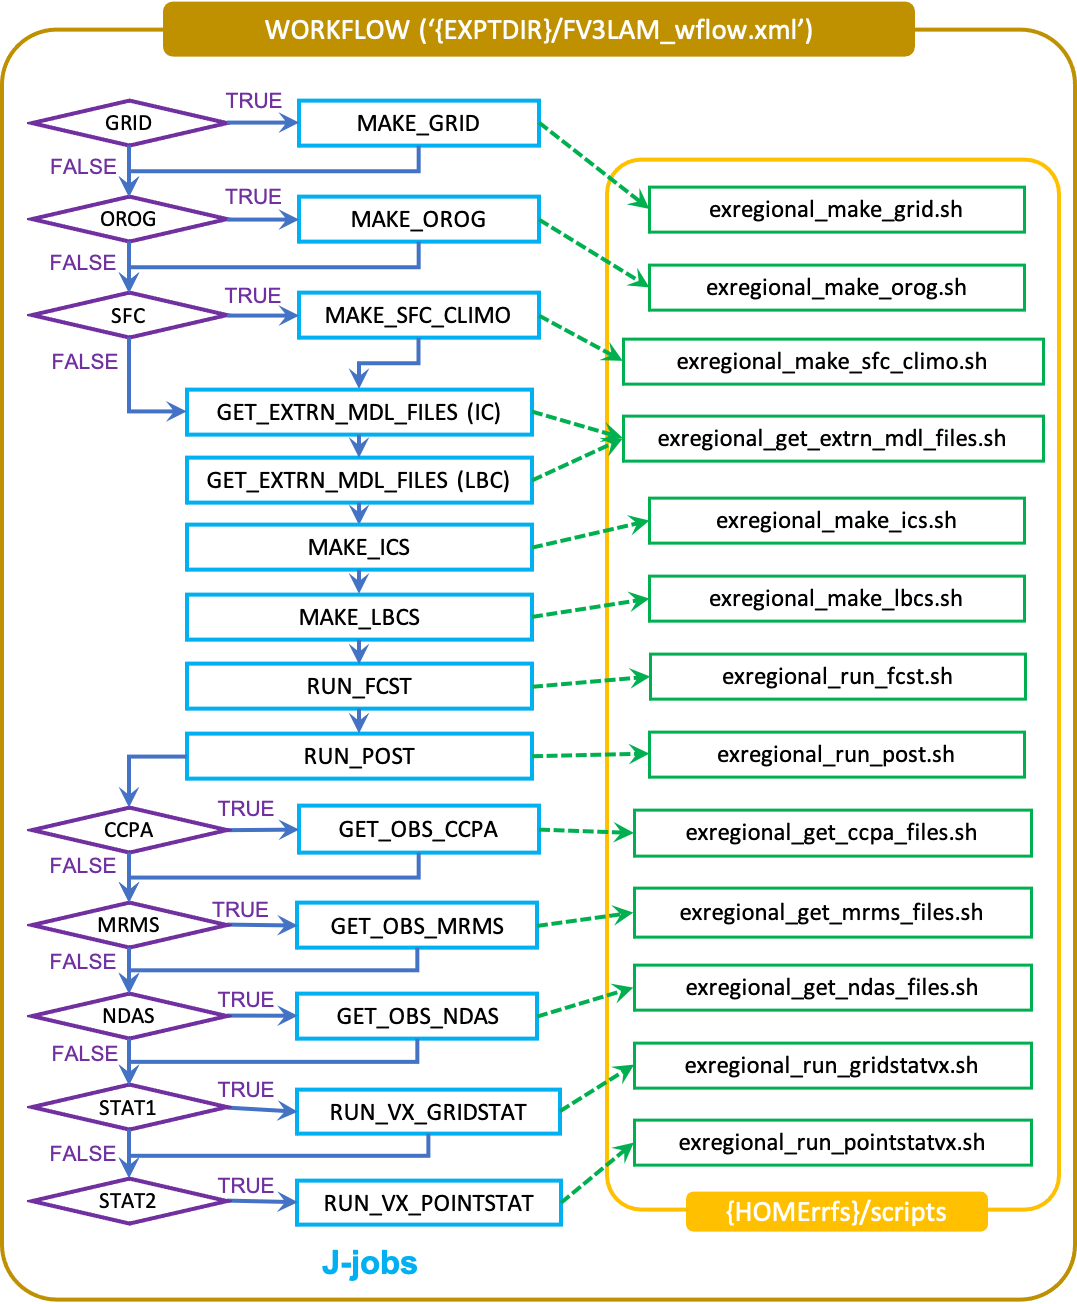
\includegraphics[width=0.7\linewidth]{FV3LAM_wflow_flowchart.png}
  \caption{Structure of the regional workflow}
  \label{fig:workflow_chart}
\end{figure}

The flowchart of the regional workflow described in `FV3LAM\_wflow.xml' is shown in Figure \ref{fig:workflow_chart}. Each task calls its own J-job script in `\{HOMErrfs\}/jobs/', and the J-job script calls its main script `exregional\_[task name].sh' located in `\{HOMErrfs\}/scripts/'. The first three pre-processing tasks; `make\_grid', `make\_orog', and `make\_sfc\_climo' are optional as described in Section \ref{subsec:turn_cycle_independent}. If the pre-generated grid, orography, and surface climatology fix files exist, these three task can be skipped by setting the corresponding flags to ``FALSE'' in the `\{HOMErrfs\}/ush/config.sh' script before running the `generate\_FV3LAM\_wflow.sh' script. In the same manner, the last five tasks; `get\_obs\_ccpa', `get\_obs\_mrms', `get\_obs\_ndas', `run\_vx\_gridstat', and `run\_vx\_pointstat' that are related to the enhanced Model Evaluation Tools (METplus) verification system can be selected separately. 

{
\fontsize{10}{12}\selectfont
\begin{longtable}{p{0.15\linewidth} | p{0.6\linewidth}  | p{0.13\linewidth} }
\hline
\hline
 Workflow task & Description & Detail \\
\hline
make\_grid & Generate regional grid files & Section \ref{sec:sar_wflow_grd_esg_gfdl}  \\
make\_orog & Generate regional orography files & Section \ref{sec:sar_wflow_oro} \\
make\_sfc\_climo & Generate surface climatology files & Section \ref{sec:sar_wflow_static} \\
get\_extrn\_ics & Obtain external data for initial conditions &  Section \ref{sec:wflow_extrn_mdl_data} \\
get\_extrn\_lbcs & Obtain external data for lateral boundary conditions & Section \ref{sec:wflow_extrn_mdl_data} \\
make\_ics & Generate initial conditions from the external data & Section \ref{sec:glb2reg_cold} \\
make\_lbcs & Generate lateral boundary conditions from the external data & Section \ref{sec:glb2reg_bndr} \\
run\_fcst & Run the forecast model (UFS weather model) & Section \ref{sec:workflow_exp_fix_dir} \\
run\_post & Run the post-processing tool {\it UPP} & Section \ref{sec:post_grb2} \\
get\_obs\_ccpa & Pull CCPA observation data for comparison & \\
get\_obs\_mrms & Pull MRMS observation data for comparison & \\
get\_obs\_ndas & Pull NDAS observation data for comparison & \\
run\_vx\_gridstat & Run METplus for grid-stat on the UPP output files & \\
run\_vx\_pointstat & Run METplus for point-stat on the UPP output files & \\
\hline
\caption{Workflow tasks}
\label{table:wflow_tasks}
\end{longtable}
}

Table \ref{table:wflow_tasks} describes the tasks in the regional workflow. You can find the detail of the workflow tasks in the specific sections of this document except for the `run\_fcst' task. As shown in Figure \ref{fig:workflow_run_fcst}, the `run\_fcst' task plays a role in collecting input files and running the FV3-LAM model as follows:
\begin{enumerate}
\item Rename the input fix files to the exact names required by the FV3-LAM model.
\item Link the input files such as `data\_table', `field\_table', `nems.configure', and `input.nml' to the experiment directory.
\item Run the FV3-LAM model.
\end{enumerate}

\begin{figure}[ht!]
  \centering
  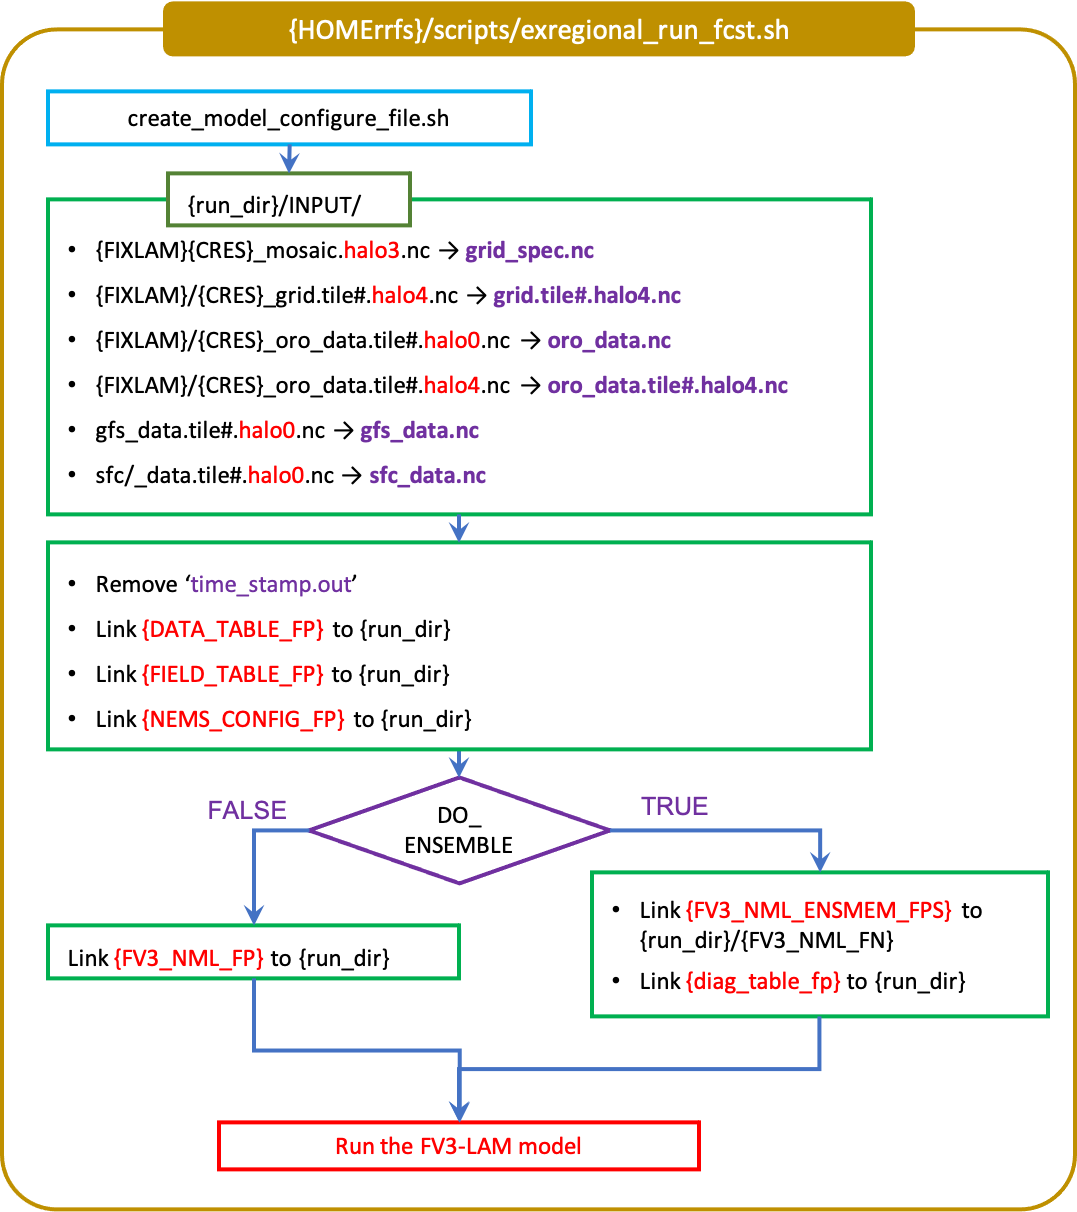
\includegraphics[width=0.7\linewidth]{FV3LAM_wflow_run_fcst.png}
  \caption{Flowchart of `exregional\_run\_fcst.sh'}
  \label{fig:workflow_run_fcst}
\end{figure}




%=================================================== 
\section{Optional Workflow Tasks}
\label{sec:wflow_select}

%---------------------------------------------------------
\subsection{Grid, Orography, and Surface Climatology}
\label{subsec:turn_cycle_independent}

The first three tasks of the workflow (`make\_grid', `make\_orog', and `make\_sfc\_climo') generate FIX files that are not cycle dependent. These tasks are not necessary for each cycle or for the `nco' mode that utilizes the pre-generated FIX files of grid, orography, and surface climatology. The following three parameters determine whether or not each of these tasks runs in the workflow:
\begin{enumerate}
\item RUN\_TASK\_MAKE\_GRID
\item RUN\_TASK\_MAKE\_OROG
\item RUN\_TASK\_MAKE\_SFC\_CLIMO
\end{enumerate}

By default, these are set to ``TRUE'' in `\{HOMErrfs\}/ush/config\_defaults.sh' as follows:
\lstset{language=bash}   
\begin{lstlisting}[frame=trBL]
RUN_TASK_MAKE_GRID="TRUE"
RUN_TASK_MAKE_OROG="TRUE"
RUN_TASK_MAKE_SFC_CLIMO="TRUE"
\end{lstlisting}

In this case, these tasks will run {\bf only once} at the beginning of the workflow before any cycle-dependent tasks are launched. They will generate grid, filtered orography, and surface climatology files that are needed by the subsequent cycle-dependent tasks.\\

If you’re running a set of cycles for which you’ve already generated these files (e.g. from a previous end-to-end run of the workflow), then you can skip these three tasks by setting the above flags to ``FALSE'' in your `config.sh' file, i.e.
\lstset{language=bash}   
\begin{lstlisting}[frame=trBL]
RUN_TASK_MAKE_GRID="FALSE"
RUN_TASK_MAKE_OROG="FALSE"
RUN_TASK_MAKE_SFC_CLIMO="FALSE"
\end{lstlisting}

In this case, you also need to specify the directories in which the workflow should look for your pre-generated grid, orography, and surface climatology files.  These directories are specified in the following three experiment parameters:
\begin{enumerate}
\item GRID\_DIR
\item OROG\_DIR
\item SFC\_CLIMO\_DIR
\end{enumerate}

Thus, to skip the `make\_grid', `make\_orog', and `make\_sfc\_climo' tasks, you would set the above three `RUN\_TASK\_MAKE\_[task]' flags to ``FALSE'' and specify the paths to your pre-generated files in your `\{HOMErrfs\}/ush/config.sh' file as follows:
\lstset{language=bash}   
\begin{lstlisting}[frame=trBL]
RUN_TASK_MAKE_GRID="FALSE"
GRID_DIR="/path/to/pre-generated/grid/files"
RUN_TASK_MAKE_OROG="FALSE"
OROG_DIR="/path/to/pre-generated/orog/files"
RUN_TASK_MAKE_SFC_CLIMO="FALSE"
SFC_CLIMO_DIR="/path/to/pre-generated/surface/climo/files"
\end{lstlisting}

{\bf Note)} If `RUN\_TASK\_MAKE\_GRID' is set to ``TRUE'', the value of `GRID\_DIR' which is set in either `config\_defaults.sh' or in `config.sh' is ignored. The same is true for `RUN\_TASK\_MAKE\_OROG' and `OROG\_DIR' and for `RUN\_TASK\_MAKE\_SFC\_CLIMO' and `SFC\_CLIMO\_DIR'.  \\

You can choose to skip any one or any two of these three tasks instead of all three.  For example, you can skip the `make\_grid' and `make\_orog' tasks but run the `make\_sfc\_climo' task by:
\begin{enumerate}
\item Set `RUN\_TASK\_MAKE\_GRID'=``FALSE'' and `RUN\_TASK\_MAKE\_OROG'=``FALSE'' in your `config.sh'.
\item Set `GRID\_DIR' and `OROG\_DIR' in your `config.sh' to the locations in which grid and orography files for the grid you want to run on can be found.
\item Set `RUN\_TASK\_MAKE\_SFC\_CLIMO'=``TRUE'' in your `config.sh' (and not setting `SFC\_CLIMO\_DIR' in `config.sh' since its value will not be used).
\end{enumerate}



%---------------------------------------------------------
\subsection{Observation Data}
\label{subsec:turn_observation_tasks}

The following three parameters determine whether or not each of the observation data tasks for CCPA, MRMS, and NDAS runs in the workflow:
\begin{enumerate}
\item RUN\_TASK\_GET\_OBS\_CCPA: Climatology-Calibrated Precipitation Analysis 
\item RUN\_TASK\_GET\_OBS\_MRMS: Multi-Radar / Multi-Sensor
\item RUN\_TASK\_GET\_OBS\_NDAS: North American Model (NAM) Data Assimilation System
\end{enumerate}

By default, these are set to ``FALSE'' in `\{HOMErrfs\}/ush/config\_defaults.sh' as follows:
\lstset{language=bash}   
\begin{lstlisting}[frame=trBL]
RUN_TASK_GET_OBS_CCPA="FALSE"
RUN_TASK_GET_OBS_MRMS="FALSE"
RUN_TASK_GET_OBS_NDAS="FALSE"
\end{lstlisting}

In either case (``TRUE'' or ``FALSE''), the paths to the observation data should be set in the configuration file to run the METplus workflow tasks as follows:
\lstset{language=bash}   
\begin{lstlisting}[frame=trBL]
CCPA_OBS_DIR="/path/to/the/ccpa/data"
MRMS_OBS_DIR="/path/to/the/mrms/data"
NDAS_OBS_DIR="/path/to/the/ndas/data"
\end{lstlisting}



%---------------------------------------------------------
\subsection{METplus}
\label{subsec:turn_metplus_tasks}

The following two parameters determine whether or not each of the METplus tasks runs in the workflow:
\begin{enumerate}
\item RUN\_TASK\_VX\_GRIDSTAT
\item RUN\_TASK\_VX\_POINTSTAT
\end{enumerate}

By default, these are set to ``FALSE'' in `\{HOMErrfs\}/ush/config\_defaults.sh' as follows:
\lstset{language=bash}   
\begin{lstlisting}[frame=trBL]
RUN_TASK_VX_GRIDSTAT="FALSE"
RUN_TASK_VX_POINTSTAT="FALSE"
\end{lstlisting}

To add the METplus tasks to the workflow:
\lstset{language=bash}   
\begin{lstlisting}[frame=trBL]
RUN_TASK_VX_GRIDSTAT="TRUE"
RUN_TASK_VX_POINTSTAT="TRUE"
\end{lstlisting}




%=================================================== 
\section{Modules for Workflow Tasks}
\label{sec:workflow_modulefiles}

The modules that are required for each task of the regional workflow are specified in:
\lstset{language=bash}   
\begin{lstlisting}[frame=trBL]
vim {HOMErrfs}/modulefiles/tasks/[machine]/[task].local
\end{lstlisting}

Each file should have a header as follows:
\lstset{language=bash}   
\begin{lstlisting}[frame=trBL]
#%Module
\end{lstlisting}

{\bf Note)} If any specific modules are not necessary for a task, the module file `[task].local' for the task will not have to exist in the directory.



%=================================================== 
\section{Launch of Workflow: `community' Mode}
\label{sec:workflow_launch_community}

There are two ways to launch the workflow: (1) using the `launch\_FV3LAM\_wflow.sh' script, and (2) manually calling the {\it rocotorun} command as follows: \\

{\bf Note)} If the {\it Python} environment for workflow is not loaded, load it as described in Section \ref{subsec:wflow_flowchart}.


%---------------------------------------------------------
\subsection{Launch with the `launch\_FV3LAM\_wflow.sh' Script}
\label{subsec:launch_script}

To launch the `launch\_FV3LAM\_wflow.sh' script, simply call it without any arguments. 
\lstset{language=bash}   
\begin{lstlisting}[frame=trBL]
cd {EXPTDIR}
./launch_FV3LAM_wflow.sh
\end{lstlisting}

This script will create (or append to if it already exists) a log file named `log.launch\_FV3LAM\_wflow' in \{EXPTDIR\}. You can check the contents towards the end of this log file (e.g. the last 30 lines) using the command:

\lstset{language=bash}   
\begin{lstlisting}[frame=trBL]
tail -n 30 log.launch_FV3LAM_wflow
\end{lstlisting}

After only one call to `launch\_FV3LAM\_wflow.sh', the {\it tail} command will output something like the following:

\lstset{language=bash}   
\begin{lstlisting}[frame=trBL, basicstyle=\tiny]

           CYCLE                        TASK                                JOBID                    STATE         EXIT STATUS      TRIES         DURATION
====================================================================================================
202006170000                make_grid         druby://hfe01:33728          SUBMITTING                             -                0                       0.0
202006170000               make_orog                                       -                                -                              -                -           	      -
202006170000       make_sfc_climo                                       -                                -                              -                -             	         -
202006170000            get_extrn_ics         druby://hfe01:33728          SUBMITTING                             -                0                       0.0
202006170000          get_extrn_lbcs         druby://hfe01:33728          SUBMITTING                             -                0                       0.0
202006170000                  make_ics                                       -                                -                              -                -              	        -
202006170000                make_lbcs                                       -                                -                              -                -                         -
202006170000                    run_fcst                                       -                                -                              -                -                         -
202006170000             run_post_00                                       -                                -                              -                -           	      -
202006170000             run_post_01                                       -                                -                              -                -            	      -
202006170000             run_post_02                                       -                                -                              -                -            	      -
202006170000             run_post_03                                       -                                -                              -                -            	      -
202006170000             run_post_04                                       -                                -                              -                -            	      -
202006170000             run_post_05                                       -                                -                              -                -            	      -
202006170000             run_post_06                                       -                                -                              -                -            	      -

Summary of workflow status:
~~~~~~~~~~~~~~~~~~~~~~~~~~

  0 out of 1 cycles completed.
  Workflow status:  IN PROGRESS

\end{lstlisting}

This shows that the `make\_grid' task (which is cycle-independent and thus run at most once per experiment regardless of the number of cycles specified in `config.sh') as well as the `get\_extrn\_ics' and `get\_extrn\_lbcs' tasks (which are cycle-dependent and thus must be run for each cycle; here, they are being run for the first cycle starting on 202006170000) are being submitted to the batch system. The overall status of the workflow is ``IN PROGRESS''. \\

Check if any tasks have error messages:
\lstset{language=bash}   
\begin{lstlisting}[frame=trBL]
cd {EXPTDIR}/log/
grep -n -i error *.log
\end{lstlisting}

\begin{itemize}
\item {\bf Note)} You can check the status of the run directly as follows:
\lstset{language=bash}   
\begin{lstlisting}[frame=trBL]
watch -n 5 squeue -u [UserID]
\end{lstlisting}
This command prints out the status of queues by [UserID] every 5 seconds.
\end{itemize}

\vspace{0.5cm}


In order to launch more tasks in the workflow, we must now call the launch script again. We can combine the call to this script with the {\it tail} command to see output from its log file into one line as follows:

\lstset{language=bash}   
\begin{lstlisting}[frame=trBL]
cd {EXPTDIR}
./launch_FV3LAM_wflow.sh ; tail -n 30 log.launch_FV3LAM_wflow
\end{lstlisting}

The output from this is something like:

\lstset{language=bash}   
\begin{lstlisting}[frame=trBL, basicstyle=\tiny]

           CYCLE                        TASK                                JOBID                    STATE         EXIT STATUS      TRIES         DURATION
====================================================================================================
202006170000                make_grid                            8794245            SUCCEEDED                             -                1                       4.0
202006170000               make_orog         druby://hfe01:33728           SUBMITTING                             -                0                       0.0
202006170000       make_sfc_climo                                       -                                -                              -                -             	           -
202006170000            get_extrn_ics                           8794246            SUCCEEDED                             -                1                      47.0
202006170000          get_extrn_lbcs                           8794246            SUCCEEDED                             -                1                      61.0
202006170000                  make_ics                                       -                                -                              -                -              	        -
202006170000                make_lbcs                                       -                                -                              -                -                         -
202006170000                    run_fcst                                       -                                -                              -                -                         -
202006170000             run_post_00                                       -                                -                              -                -           	      -
202006170000             run_post_01                                       -                                -                              -                -            	      -
202006170000             run_post_02                                       -                                -                              -                -            	      -
202006170000             run_post_03                                       -                                -                              -                -            	      -
202006170000             run_post_04                                       -                                -                              -                -            	      -
202006170000             run_post_05                                       -                                -                              -                -            	      -
202006170000             run_post_06                                       -                                -                              -                -            	      -

Summary of workflow status:
~~~~~~~~~~~~~~~~~~~~~~~~~~

  0 out of 1 cycles completed.
  Workflow status:  IN PROGRESS

\end{lstlisting}

This shows that the `make\_grid' task as well as `get\_extrn\_ics' and `get\_extrn\_lbcs' tasks for the 202006170000 cycle have completed successfully and that the `make\_orog' task (which is cycle-independent and thus run at most once per experiment regardless of the number of cycles specified in `config.sh') is being submitted to the batch system. \\

Once the pre-processing tasks complete without any errors, you should find the files representing completion of the tasks in `\{EXPTDIR\}/log/' as follows:
{
\fontsize{10}{12}\selectfont
\begin{longtable}{ p{0.2\linewidth} | p{0.4\linewidth} }
\hline
\hline
 Task & File of completion \\
\hline
 make\_grid & make\_grid\_task\_complete.txt \\
 make\_orog & make\_orog\_task\_complete.txt \\
 make\_sfc\_climo & make\_sfc\_climo\_task\_complete.txt \\ 
\hline
\caption{File names representing completion of the pre-processing tasks }
\label{table:wflow_fn_taskcomplete}
\end{longtable}
}


{\bf Note)} You can call the launch script as often as you like, i.e. you do not have to wait until the currently running tasks are finished. If they are still running, the script will simply append to the log file a new table (which is generated using {\it Rocoto}'s {\it rocotostat} command) listing the state of any running tasks as ``RUNNING''. \\

Once the `make\_grid', `make\_orog', and `make\_sfc\_climo' tasks and the `get\_extrn\_ics' and `get\_extrn\_lbcs' tasks for the 202006170000 cycle have completed successfully, the new files and sub-directories are as follows:

{
\fontsize{10}{12}\selectfont
\begin{longtable}{p{0.03\linewidth} | p{0.26\linewidth} | p{0.6\linewidth} }
\hline
\hline
No. & Directory/file name & Description \\
\hline
1 & 2020061700 & This is the directory created when the first cycle-specific workflow tasks are run, which are `get\_extrn\_ics' and `get\_extrn\_lbcs' (they are launched simultaneously for each cycle in the experiment). We refer to this as a ``cycle directory''. Cycle directories are created to contain cycle-specific files for each cycle that the experiment runs. If `DATE\_FIRST\_CYCL' and `DATE\_LAST\_CYCL' were different, and/or `CYCL\_HRS' contained more than one element in the `config.sh' file, then more than one cycle directory would be created under the experiment directory. \\
2 & grid & This is a directory generated by the `make\_grid' task. It contains the grid files for the experiment. \\
3 & log & This is a directory in which the log files generated by the overall workflow as well as its various tasks are stored. Look in these files to trace why a task may have failed. \\
4 & orog & This is a directory generated by the `make\_orog' task. It contains the orography files for the experiment. \\
5 & sfc\_climo & This is a directory generated by the `make\_sfc\_climo' task. It contains the surface climatology files for the experiment. \\
\hdashline
6 & FV3LAM\_wflow.db  FV3LAM\_wlfow\_lock.db & These are database files that are generated with {\it rocoto} is called (by the launch script) to launch the workflow. There is usually no need for the user to modify these files. If you relaunch the workflow from scratch, {\bf delete} these files and then call the launch script (multiple times, as usual). \\
7 & log.launch\_FV3LAM\_wflow & This is the log file to which the launch script (`launch\_FV3LAM\_ wflow.sh') appends its output each time it is called. Take a look at the last 30--50 lines of this file to check the status of the workflow. \\
\hline
\caption{New directories and files created by {\it Rocoto} }
\label{table:wflow_udef_dir}
\end{longtable}
}

{\bf Notes)} To avoid having to manually call the launch script, the experiment generation script allows users to automatically place the call to this script in the user's crontab and have {\it cron} call it with a specified frequency. \\

If everything goes smoothly, you will eventually get the following workflow status table as follows:
\lstset{language=bash}   
\begin{lstlisting}[frame=trBL, basicstyle=\tiny]

           CYCLE                        TASK                                JOBID                    STATE         EXIT STATUS      TRIES         DURATION
====================================================================================================
202006170000                make_grid                            8854765            SUCCEEDED                             0                1                       6.0
202006170000               make_orog                            8854809            SUCCEEDED                             0                1                     27.0
202006170000       make_sfc_climo                            8854849            SUCCEEDED                             0                1             	     36.0
202006170000            get_extrn_ics                            8854763            SUCCEEDED                             0                1                     54.0
202006170000          get_extrn_lbcs                            8854764            SUCCEEDED                             0                1                     61.0
202006170000                  make_ics                            8854914            SUCCEEDED                             0                1                   119.0
202006170000                make_lbcs                            8854913            SUCCEEDED                             0                1                     98.0
202006170000                    run_fcst                            8854992            SUCCEEDED                              0               1                   655.0
202006170000             run_post_00                            8855459            SUCCEEDED                             0                1                       6.0
202006170000             run_post_01                            8855460            SUCCEEDED                             0                1                       6.0
202006170000             run_post_02                            8855461            SUCCEEDED                             0                1                       6.0
202006170000             run_post_03                            8855462            SUCCEEDED                             0                1                       6.0
202006170000             run_post_04                            8855463            SUCCEEDED                             0                1                       6.0
202006170000             run_post_05                            8855464            SUCCEEDED                             0                1                       6.0
202006170000             run_post_06                            8855465            SUCCEEDED                             0                1                       6.0

\end{lstlisting}


If all the tasks are completed successfully, the workflow status in this log file will be set to ``SUCCESS''. If one or more tasks are not completed successfully for some reason, the workflow status will be set to ``FAILURE''.

\lstset{language=bash}   
\begin{lstlisting}[frame=trBL]
The end-to-end run of the workflow for the forecast experiment specified 
by expt_name has completed with the following workflow status (wflow_-
status):
  expt_name = "test_community_hrrr25"
  wflow_status = "SUCCESS"
  
\end{lstlisting}



%---------------------------------------------------------
\subsection{Launch Manually by Calling the {\it rocotorun} Command}
\label{subsec:launch_manual}

Load the {\it Rocoto} module if it is not loaded:
\begin{itemize}
\item Hera:
\lstset{language=bash}   
\begin{lstlisting}[frame=trBL]
module load rocoto
\end{lstlisting}

\item WCOSS\_DELL\_P3:
\lstset{language=bash}   
\begin{lstlisting}[frame=trBL]
module load lsf/10.1
module use /gpfs/dell3/usrx/local/dev/emc_rocoto/modulefiles/
module load ruby/2.5.1 rocoto/1.2.4
\end{lstlisting}

\item WCOSS\_CRAY:
\lstset{language=bash}   
\begin{lstlisting}[frame=trBL]
module load xt-lsfhpc/9.1.3
module use -a /usrx/local/emc_rocoto/modulefiles
module load rocoto/1.2.4
\end{lstlisting}

\end{itemize}


Launch the workflow as follows:
\lstset{language=bash}   
\begin{lstlisting}[frame=trBL]
cd {EXPTDIR}
rocotorun -w FV3LAM_wflow.xml -d FV3LAM_wflow.db -v 10
\end{lstlisting}
where `\{EXPTDIR\}' is the user-defined experimental directory. \\

To see the status of the workflow, issue a {\it rocotostat} command as follows:
\lstset{language=bash}   
\begin{lstlisting}[frame=trBL]
cd {EXPTDIR}
rocotostat -w FV3LAM_wflow.xml -d FV3LAM_wflow.db -v 10
\end{lstlisting}

Wait a few seconds and issue a second set of {\it rocotorun} and {\it rocotostat} commands as follows:
\lstset{language=bash}   
\begin{lstlisting}[frame=trBL]
rocotorun -w FV3LAM_wflow.xml -d FV3LAM_wflow.db -v 10
rocotostat -w FV3LAM_wflow.xml -d FV3LAM_wflow.db -v 10
\end{lstlisting}

{\bf Note)} Issuing a 2nd (3rd, etc) {\it rocotostat} command without an intervening {\it rocotorun} command will not result in an updated workflow status table. It is the {\it rocotorun} command that updates the workflow database file (in this case `FV3LAM\_wflow.db', located in \{EXPTDIR\}). The {\it rocotostat} command just reads the database file and prints the table to the screen.  Thus, to see an updated table, you must always first issue a {\it rocotorun} command and then follow it up with a {\it rocotostat} command.



%---------------------------------------------------------
\subsection{How to Restart a `DEAD' Task}
\label{subsec:restart_dead_task}

When something goes wrong, a workflow task would end up in the `DEAD' state as follows:

\lstset{language=bash}   
\begin{lstlisting}[frame=trBL]
rocotostat -w FV3LAM_wflow.xml -d FV3LAM_wflow.db -v 10
       CYCLE            TASK        JOBID    STATE    EXIT STATUS  TRIES DURATION
=================================================================================
201906150000       make_grid      9443237   QUEUED              -      0      0.0
201906150000       make_orog            -        -              -      -        -
201906150000  make_sfc_climo            -        -              -      -        -
201906150000   get_extrn_ics      9443293     DEAD            256      3      5.0
\end{lstlisting}

Once the issue has been resolved, the failed task can re-run using the `rocotorewind' command (See \ref{sec:rocoto}):

\lstset{language=bash}   
\begin{lstlisting}[frame=trBL]
rocotorewind -w FV3LAM_wflow.xml -d FV3LAM_wflow.db -v 10 -c 201906150000 -t get_extrn_ics
\end{lstlisting}
where 
{
\fontsize{10}{12}\selectfont
\begin{longtable}{p{0.06\linewidth} | p{0.64\linewidth} }
\hline
\hline
Flag & Description \\
\hline
-w & Path to workflow XML file (`FV3LAM\_wflow.xml') \\
-d & Path to workflow database file (`FV3LAM\_wflow.db') \\
-v & Run Rocoto in verbose mode [LEVEL] \\
-c & List of cycles (YYYYMMDDHHmm) `c1,c2,c3' or `c1:c2' or all \\
-t & List of tasks `a,b,c' \\
\hline
\caption{Flags for the `rocotorewind' command}
\label{table:rocotorewind_flag}
\end{longtable}
}

{\bf Note)} The name of cycle with `-c' must include Minutes (mm).


%---------------------------------------------------------
\subsection{How to Re-run Forecast and Post Tasks Only }
\label{subsec:rerun_fcst_post}

There are two approaches to run the forecast and post tasks again after modification of the source code: (1) Using {\it rocotorewind}, and (2) Modifying `FV3LAM\_wflow.xml'.

\begin{enumerate}

\item Use the {\it rocotorewind} command to undo the tasks as described in Section \ref{subsec:restart_dead_task}.

\begin{enumerate}
\item Load the {\it rocoto} module as described in Section \ref{subsec:launch_manual}.

\item Remove the result files generated by the previous forecast and post tasks:
\lstset{language=bash}   
\begin{lstlisting}[frame=trBL]
cd {EXPTDIR}/{CYCLE}
rm -f atmos_4xdaily.nc atmos_static.nc
rm -f dynf* logf* phyf*
rm -rf postprd
\end{lstlisting}

\item Run {\it rocotorewind} for the forecast and post tasks:
\lstset{language=bash}   
\begin{lstlisting}[frame=trBL]
rocotorewind -w FV3LAM_wflow.xml -d FV3LAM_wflow.db -v 10 -c 201906150000 -t 'run_fcst,run_post_f001,run_post_f002,run_post_f003,run_post_f004,run_post_f005,run_post_f006'
\end{lstlisting}

\item Run the forecast and post tasks again:
\lstset{language=bash}   
\begin{lstlisting}[frame=trBL]
./launch_FV3LAM_wflow.sh
\end{lstlisting}
\end{enumerate}


\item Modify the workflow XML file `FV3LAM\_wflow.xml'.

\begin{enumerate}
\item Remove the result files generated by the previous forecast and post tasks:
\lstset{language=bash}   
\begin{lstlisting}[frame=trBL]
cd {EXPTDIR}/{CYCLE}
rm -f atmos_4xdaily.nc atmos_static.nc
rm -f dynf* logf* phyf*
rm -rf postprd
\end{lstlisting}

\item Remove the workflow data files:
\lstset{language=bash}   
\begin{lstlisting}[frame=trBL]
cd ..
rm -f FV3LAM_*.db
\end{lstlisting}

\item Modify the workflow XML file `FV3LAM\_wflow.xml':
\begin{itemize}
\item Remove other tasks listed below (between lines 101--319 approx.):
\begin{itemize}
\item MAKE\_GRID\_TN (``make\_grid'')
\item MAKE\_OROG\_TN (``make\_orog'')
\item MAKE\_SFC\_CLIMO\_TN (``make\_sfc\_climo'')
\item GET\_EXTRN\_ICS\_TN (``get\_extrn\_ics'')
\item GET\_EXTRN\_LBCS\_TN (``get\_extrn\_lbcs'')
\item MAKE\_ICS\_TN (``make\_ics'')
\item MAKE\_LBCS\_TN (``make\_lbcs'')
\end{itemize}

\item Remove the dependency of the `\&RUN\_FCST\_TN' task:
\lstset{language=XML}   
\begin{lstlisting}[frame=trBL,basicstyle=\tiny]
    <dependency>
      <and>
        <taskdep task="&MAKE_ICS_TN;"/>
        <taskdep task="&MAKE_LBCS_TN;"/>
      </and>
    </dependency>
\end{lstlisting}
\end{itemize}

Finally, the task part of `FV3LAM\_wflow.xml' should be as follows:
\lstset{language=XML}   
\begin{lstlisting}[frame=trBL,basicstyle=\tiny]
<workflow realtime="F" scheduler="&SCHED;" cyclethrottle="20">

  <cycledef group="at_start">00 00 15 06 2019 *</cycledef>
  <cycledef group="forecast">201906150000 201906150000 24:00:00</cycledef>

  <log>
    <cyclestr>&LOGDIR;/FV3LAM_wflow.log</cyclestr>
  </log>

<!--
************************************************************************
************************************************************************
-->
  <task name="&RUN_FCST_TN;" maxtries="1">

    &RSRV_FCST;
    <command>&LOAD_MODULES_RUN_TASK_FP; "&RUN_FCST_TN;" "&JOBSDIR;/JREGIONAL_RUN_FCST"</command>

    <cores>12</cores>
    <native>--cpus-per-task 4 --exclusive</native>

    <walltime>01:00:00</walltime>
    <jobname>&RUN_FCST_TN;</jobname>
    <join><cyclestr>&LOGDIR;/&RUN_FCST_TN;_@Y@m@d@H.log</cyclestr></join>

    <envar><name>GLOBAL_VAR_DEFNS_FP</name><value>&GLOBAL_VAR_DEFNS_FP;</value></envar>
    <envar><name>PDY</name><value><cyclestr>@Y@m@d</cyclestr></value></envar>
    <envar><name>CDATE</name><value><cyclestr>@Y@m@d@H</cyclestr></value></envar>
    <envar><name>CYCLE_DIR</name><value><cyclestr>&CYCLE_BASEDIR;/@Y@m@d@H</cyclestr></value></envar>
    <envar><name>SLASH_ENSMEM_SUBDIR</name><value><cyclestr></cyclestr></value></envar>
    <envar><name>ENSMEM_INDX</name><value><cyclestr>##</cyclestr></value></envar>

  </task>
<!--
************************************************************************
************************************************************************
-->
  <metatask name="&RUN_POST_TN;">

    <var name="fhr">  000 001 002 003 004 005 006 007 008 009 010 011 012 013 014 015 016 017 018 019 020 021 022 023 024 025 026 027 028 029 030 031 032 033 034 035 036 037 038 039 040 041 042 043 044 045 046 047 048 </var>

    <task name="&RUN_POST_TN;_f#fhr#" maxtries="1">

      &RSRV_DEFAULT;
      <command>&LOAD_MODULES_RUN_TASK_FP; "&RUN_POST_TN;" "&JOBSDIR;/JREGIONAL_RUN_POST"</command>
      <nodes>2:ppn=24</nodes>
      <walltime>00:15:00</walltime>
      <nodesize>&NCORES_PER_NODE;</nodesize>
      <jobname>&RUN_POST_TN;_f#fhr#</jobname>
      <join><cyclestr>&LOGDIR;/&RUN_POST_TN;_f#fhr#_@Y@m@d@H.log</cyclestr></join>

      <envar><name>GLOBAL_VAR_DEFNS_FP</name><value>&GLOBAL_VAR_DEFNS_FP;</value></envar>
      <envar><name>PDY</name><value><cyclestr>@Y@m@d</cyclestr></value></envar>
      <envar><name>CDATE</name><value><cyclestr>@Y@m@d@H</cyclestr></value></envar>
      <envar><name>CYCLE_DIR</name><value><cyclestr>&CYCLE_BASEDIR;/@Y@m@d@H</cyclestr></value></envar>
      <envar><name>SLASH_ENSMEM_SUBDIR</name><value><cyclestr></cyclestr></value></envar>
      <envar><name>cyc</name><value><cyclestr>@H</cyclestr></value></envar>
      <envar><name>fhr</name><value>#fhr#</value></envar>

      <dependency>
        <or>
          <taskdep task="&RUN_FCST_TN;"/>
          <and>
            <datadep age="05:00"><cyclestr>&CYCLE_BASEDIR;/@Y@m@d@H/dynf#fhr#.nc</cyclestr></datadep>
            <datadep age="05:00"><cyclestr>&CYCLE_BASEDIR;/@Y@m@d@H/phyf#fhr#.nc</cyclestr></datadep>
          </and>
        </or>
      </dependency>

    </task>

  </metatask>

\end{lstlisting}

\item Run the forecast and post tasks again:
\lstset{language=bash}   
\begin{lstlisting}[frame=trBL]
./launch_FV3LAM_wflow.sh
\end{lstlisting}
\end{enumerate}

\end{enumerate}



%=================================================== 
\section{Launch of Workflow: `nco' Mode}
\label{sec:workflow_launch_nco}

%---------------------------------------------------------
\subsection{Mosaic Halo Files}
\label{subsec:mosaic_halo}

Different from the previous EMC's regional workflow, the unified regional workflow in the short range weather application requires `mosaic\_halo3.nc' and `mosaic\_halo4.nc' files as well as `mosaic\_halo6.nc'. Previously, there was just one mosaic file `C\{res\}\_mosaic.nc' that points to the pre-shave {\bf halo6} file. A mosaic file is used by both the preprocessing codes and by {\it FV3}. Since halo6 has more layers than halo3, things will not go out of bounds but it might cause some potential issues. Therefore, it is important for each grid file to have its own mosaic file corresponding to the number of halos.

\begin{enumerate}

\item Load the modules used for build the executable `make\_solo\_mosaic':
\begin{itemize}
\item On Hera:
\lstset{language=bash}   
\begin{lstlisting}[frame=trBL]
source {HOMErrfs}/../env/build_hera_intel.env
\end{lstlisting}

\item On WCOSS\_dell\_p3:
\lstset{language=bash}   
\begin{lstlisting}[frame=trBL]
source {HOMErrfs}/../env/build_wcoss_dell_p3_intel.env
\end{lstlisting}

\item On WCOSS\_cray:
\lstset{language=bash}   
\begin{lstlisting}[frame=trBL]
source {HOMErrfs}/../env/build_wcoss_cray_intel.env
\end{lstlisting}

\item On Orion:
\lstset{language=bash}   
\begin{lstlisting}[frame=trBL]
source {HOMErrfs}/../env/build_orion_intel.env
\end{lstlisting}

\end{itemize}


\item Run the executable `make\_solo\_mosaic' for each mosaic file:
\lstset{language=bash}   
\begin{lstlisting}[frame=trBL]
cd {FIXLAM_NCO_BASEDIR}/{PREDEF_GRID_NAME}/
{BIN}/make_solo_mosaic --num_tile 1 --dir "{FIXLAM_NCO_BASEDIR}/{PREDEF_ GRID_NAME}" --tile_file "C{res}_grid.tile7.halo6.nc" --mosaic "C{res}_mosaic.halo6"
{BIN}/make_solo_mosaic --num_tile 1 --dir "{FIXLAM_NCO_BASEDIR}/{PREDEF_ GRID_NAME}" --tile_file "C{res}_grid.tile7.halo3.nc" --mosaic "C{res}_mosaic.halo3"
{BIN}/make_solo_mosaic --num_tile 1 --dir "{FIXLAM_NCO_BASEDIR}/{PREDEF_ GRID_NAME}" --tile_file "C{res}_grid.tile7.halo4.nc" --mosaic "C{res}_mosaic.halo4"
\end{lstlisting}
where `\{BIN\}' is the directory where the executable `make\_solo\_mosaic' is located (typically =`\{HOME\}/bin/'). \\

\end{enumerate}



%---------------------------------------------------------
\subsection{Launch with the `launch\_FV3LAM\_wflow.sh' Script}
\label{subsec:launch_nco}

Launch the `launch\_FV3LAM\_wflow.sh' script: 
\lstset{language=bash}   
\begin{lstlisting}[frame=trBL]
cd {EXPTDIR}
./launch_FV3LAM_wflow.sh
\end{lstlisting}

This script will create (or append to if it already exists) a log file named `log.launch\_FV3LAM\_wflow' in \{EXPTDIR\}. You can check the contents towards the end of this log file (e.g. the last 30 lines) using the command:

\lstset{language=bash}   
\begin{lstlisting}[frame=trBL]
tail -n 30 log.launch_FV3LAM_wflow
\end{lstlisting}

After only one call to `launch\_FV3LAM\_wflow.sh', the {\it tail} command will output something like the following:

\lstset{language=bash}   
\begin{lstlisting}[frame=trBL, basicstyle=\tiny]

           CYCLE                        TASK                                JOBID                    STATE         EXIT STATUS      TRIES         DURATION
====================================================================================================
202006180000            get_extrn_ics         druby://hfe01:33424          SUBMITTING                             -                0                       0.0
202006180000          get_extrn_lbcs         druby://hfe01:33424          SUBMITTING                             -                0                       0.0
202006180000                  make_ics                                       -                                -                              -                -              	        -
202006180000                make_lbcs                                       -                                -                              -                -                         -
202006180000                    run_fcst                                       -                                -                              -                -                         -
202006180000             run_post_00                                       -                                -                              -                -           	      -
202006180000             run_post_01                                       -                                -                              -                -            	      -
202006180000             run_post_02                                       -                                -                              -                -            	      -
202006180000             run_post_03                                       -                                -                              -                -            	      -
202006180000             run_post_04                                       -                                -                              -                -            	      -
202006180000             run_post_05                                       -                                -                              -                -            	      -
202006180000             run_post_06                                       -                                -                              -                -            	      -

Summary of workflow status:
~~~~~~~~~~~~~~~~~~~~~~~~~~

  0 out of 1 cycles completed.
  Workflow status:  IN PROGRESS

\end{lstlisting}


In order to launch more tasks in the workflow, we must now call the launch script again. We can combine the call to this script with the {\it tail} command to see output from its log file into one line as follows:

\lstset{language=bash}   
\begin{lstlisting}[frame=trBL]
cd {EXPTDIR}
./launch_FV3LAM_wflow ; tail -n 30 log.launch_FV3LAM_wflow
\end{lstlisting}

The output from this is something like:

\lstset{language=bash}   
\begin{lstlisting}[frame=trBL, basicstyle=\tiny]

           CYCLE                        TASK                                JOBID                    STATE         EXIT STATUS      TRIES         DURATION
====================================================================================================
201909011800            get_extrn_ics                            8887541           SUCCEEDED                             0                1                       4.0
201909011800          get_extrn_lbcs                            8887542           SUCCEEDED                             0                1                       4.0
201909011800                  make_ics         druby://hfe11:33475           SUBMITTING                            -                0              	    0.0
201909011800                make_lbcs         druby://hfe11:33475           SUBMITTING                            -                0                       0.0
201909011800                    run_fcst                                       -                                -                              -                -                         -
201909011800             run_post_00                                       -                                -                              -                -           	      -
201909011800             run_post_01                                       -                                -                              -                -            	      -
201909011800             run_post_02                                       -                                -                              -                -            	      -
201909011800             run_post_03                                       -                                -                              -                -            	      -
201909011800             run_post_04                                       -                                -                              -                -            	      -
201909011800             run_post_05                                       -                                -                              -                -            	      -
201909011800             run_post_06                                       -                                -                              -                -            	      -

\end{lstlisting}

If everything goes smoothly, you will eventually get the following workflow status table as follows:
\lstset{language=bash}   
\begin{lstlisting}[frame=trBL, basicstyle=\tiny]

           CYCLE                        TASK                                JOBID                    STATE         EXIT STATUS      TRIES         DURATION
====================================================================================================
201909011800            get_extrn_ics                            8887541            SUCCEEDED                             0                1                     2.0
201909011800          get_extrn_lbcs                            8887542            SUCCEEDED                             0                1                     2.0
201909011800                  make_ics                            8887551            SUCCEEDED                             0                1                   160.0
201909011800                make_lbcs                            8887552            SUCCEEDED                             0                1                   148.0
201909011800                    run_fcst                            8887753            SUCCEEDED                              0               1                   365.0
201909011800             run_post_00                            8888085            SUCCEEDED                             0                1                       7.0
201909011800             run_post_01                            8888086            SUCCEEDED                             0                1                       7.0
201909011800             run_post_02                            8888087            SUCCEEDED                             0                1                       8.0
201909011800             run_post_03                            8888106            SUCCEEDED                             0                1                       6.0
201909011800             run_post_04                            8888107            SUCCEEDED                             0                1                       7.0
201909011800             run_post_05                            8888108            SUCCEEDED                             0                1                       8.0
201909011800             run_post_06                            8888109            SUCCEEDED                             0                 1                      6.0

\end{lstlisting}

If all the tasks completed successfully, the workflow status in this log file will be set to ``SUCCESS''. If for some reason one or more tasks did not complete successfully, the workflow status will be set to ``FAILURE''.

\lstset{language=bash}   
\begin{lstlisting}[frame=trBL]
The end-to-end run of the workflow for the forecast experiment specified 
by expt_name has completed with the following workflow status (wflow_-
status):
  expt_name = "test_nco_conus96"
  wflow_status = "SUCCESS"
\end{lstlisting}




%=================================================== 
\section{Automatic Resubmission with Cron}                 
\label{sec:auto_resub_cron}

%---------------------------------------------------------
\subsection{Syntax of Crontab}
\label{subsec:cron_syntax}

Cron runs jobs at designated times and intervals periodically. Cron is controlled by a `crontab' file.  Each line in a crontab file represents a separate job, and it has five time components followed by a shell command to execute as follows:

\lstset{language=bash}   
\begin{lstlisting}[frame=trBL]
A B C D E <command to execute>
\end{lstlisting}
where `A' is minute (0--59), `B' is hour (0--23), `C' is day of the month (1--31), `D' is month (1--12), and `E' is day of the week (0--6 which mean Sunday--Saturday). \\

{\bf Notes)}
\begin{itemize}
\item `*': Run for every time.
\item `*/n' : Run for every n-th interval of time.
\item Multiple specific time intervals can be specified with commas (`,').
\item `-': Range of values.
\item Comments begin with a comment mark `\#'.
\end{itemize}

For example, the below would run `my\_script.sh' every 10 minutes of every first, second, and third hour between the 10th and 15th of every month:
\lstset{language=bash}   
\begin{lstlisting}[frame=trBL]
*/10 1,2,3 10-15 * * /scratch2/NCEPDEV/fv3-cam/Chan-hoo.Jeon/my_script.sh
\end{lstlisting}


%---------------------------------------------------------
\subsection{Setting up Command Line on Hera / WCOSS Cray}
\label{subsec:cron_command_cray}

There are two ways to set up a command line in the cron: 1) using a command line, and 2) putting a command line in a file.
\begin{enumerate}
\item Using a command line:

Open a crontab editor (vim):
\lstset{language=bash}   
\begin{lstlisting}[frame=trBL]
crontab -e
\end{lstlisting}

Put a command line:
\lstset{language=bash}   
\begin{lstlisting}[frame=trBL]
*/10 1,2,3 * * * /scratch2/NCEPDEV/fv3-cam/Chan-hoo.Jeon/my_script.sh
\end{lstlisting}

Check the crontab:
\lstset{language=bash}   
\begin{lstlisting}[frame=trBL]
crontab -l
\end{lstlisting}

You can remove the crontab as follows:
\lstset{language=bash}   
\begin{lstlisting}[frame=trBL]
crontab -r
\end{lstlisting}


\item Putting a command in a file:

Open a file:
\lstset{language=bash}   
\begin{lstlisting}[frame=trBL]
vim my_crontab.txt
\end{lstlisting}

Put a command line:
\lstset{language=bash}   
\begin{lstlisting}[frame=trBL]
*/10 1,2,3 * * * /scratch2/NCEPDEV/fv3-cam/Chan-hoo.Jeon/my_script.sh
\end{lstlisting}

Put it in the cron:
\lstset{language=bash}   
\begin{lstlisting}[frame=trBL]
crontab my_crontab.txt
\end{lstlisting}

\end{enumerate}



%---------------------------------------------------------
\subsection{Setting up Command Line on WCOSS Dell}
\label{subsec:cron_command_dell}

The `crontab' command, described in Section \ref{subsec:cron_command_cray}, does not work on the WCOSS Dell. Instead, a directory named `cron' exists in the home directory as `/u/Chan-Hoo.Jeon/cron'. In this directory, you can find a `mycrontab' file where command lines are added like the second approach of Section \ref{subsec:cron_command_cray}. The difference is that you do not have to type `crontab' here. 

\vspace{0.3cm}

Open a file:
\lstset{language=bash}   
\begin{lstlisting}[frame=trBL]
cd /u/Chan-Hoo.Jeon/cron
vim mycrontab
\end{lstlisting}

Put a command line:
\lstset{language=bash}   
\begin{lstlisting}[frame=trBL]
*/10 1,2,3 * * * /gpfs/dell2/emc/modeling/noscrub/Chan-Hoo.Jeon/test/my_script.sh
\end{lstlisting}

\vspace{0.3cm}

{\bf Note)} it usually takes about 5 minutes to put your script in the cron, which is different from other machines where it is immediately in.



%---------------------------------------------------------
\subsection{Sample Command for Launch Script}
\label{subsec:we2e_sample_launch}

Below is a sample command to launch the script described in Sections \ref{subsec:launch_script} and \ref{subsec:launch_nco}:

\lstset{language=bash}   
\begin{lstlisting}[frame=trBL]
*/05 * * * * cd /scratch2/NCEPDEV/fv3-cam/Chan-hoo.Jeon/expt_dirs/grid_RRFS_CONUS_13km_ics_FV3GFS_lbcs_FV3GFS_suite_GFS_v15p2 && ./launch_FV3LAM_wflow.sh >> ./log.launch_FV3LAM_wflow 2>&1
\end{lstlisting}




%=================================================== 
\section{Output}                 
\label{sec:workflow_output}

%---------------------------------------------------------
\subsection{Type of Output Files}
\label{subsec:type_output}

The output files that contain the physical variables are converted into other formats such as NetCDF and GRIB2 in the regional workflow as shown in Figure \ref{fig:wflow_output_files}. The names of the raw output files, `fv3\_history' and `fv3\_history2d', are specified in the input file `diag\_table'. When `quilting' is set to `.true.' for the write components in another input file `model\_configure', the two files of `fv3\_history' and `fv3\_history2d' are converted into two types of NetCDF files named `dynf\{hhh\}.nc' and `phyf\{hhh\}.nc'. The bases of the file names, `dyn' and `phy', are specified in `model\_configure'. These NetCDF files are converted into two types of GRIB2 files named `BGDAWP' and `BGRD3D'. Finally, the `BGDAWP' and `BGRD3D' files are soft-linked to `[domain].tXXz.bgdawpf\{hhhmm\}.tmXX' and `[domain].bgrd3df\{hhhmm\}.tmXX', respectively, where \{hhhmm\} denotes simulation hours and minutes. Moreover, when the METplus option is on, additional output files are generated from the `[domain].tXXz.bgdawpf\{hhhmm\}.tmXX' and observation data. \\

In addition, the other output files `gird\_spec.nc', `atmos\_static.nc', and `atmos\_4xdaily.nc', specified in the input file `diag\_table', are independent from the above conversion. They contain the fields as follows:
\begin{enumerate}
\item `grid\_spec.nc':
{
\fontsize{10}{12}\selectfont
\begin{longtable}{p{0.12\linewidth} | p{0.65\linewidth} }
\hline
\hline
Field name & Description \\
\hline
 grid\_lon & Longitude of the bottom-left corner (index; top-right on the map) of each grid cell \\
 grid\_lat & Latitude of the bottom-left corner (index; top-right on the map) of each grid cell \\
 grid\_lont & Longitude of the center of each grid cell \\
 grid\_latt & Latitude of the center of each grid cell  \\
 area & Cell area  \\
\hline
\caption{Fields in `grid\_spec.nc'}
\label{table:fv3_out_grid_spec}
\end{longtable}
}

\item `atmos\_static.nc':
{
\fontsize{10}{12}\selectfont
\begin{longtable}{ p{0.12\linewidth} | p{0.6\linewidth} }
\hline
\hline
 Field name & Description \\
\hline
 pk & Pressure at the interface `k' (hybrid coordinate)  \\
 bk & Vertical coordinate sigma value \\
 hyam & Hybrid coefficient A at the vertical levels \\
 hybm & Hybrid coefficient B at the vertical levels  \\
 zsurf & Surface height (orography)  \\
\hline
\caption{Fields in `atmos\_static.nc'}
\label{table:fv3_out_atmos_static}
\end{longtable}
}

\item `atmos\_4xdaily.nc':
\begin{itemize}
\item Fields are specified in the input file `diag\_table'. See Section \ref{subsec:diag_table}
\end{itemize}



\end{enumerate}


\begin{figure}[ht!]
  \centering
  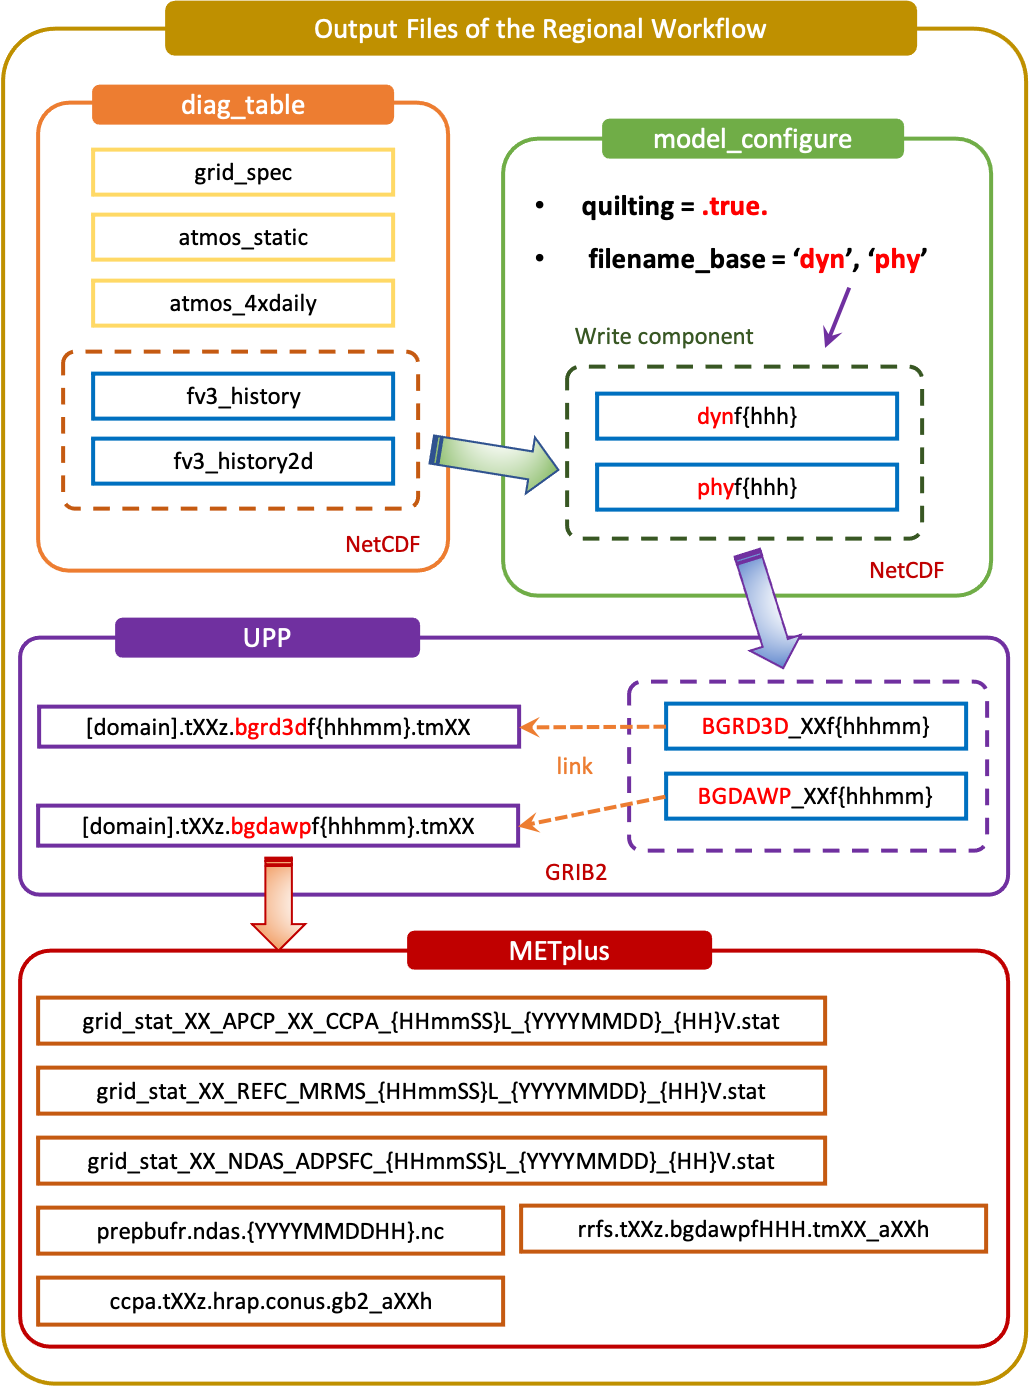
\includegraphics[width=0.67\linewidth]{FV3LAM_wflow_output_files.png}
  \caption{Output files of the regional workflow}
  \label{fig:wflow_output_files}
\end{figure}



\vspace{0.5cm}

%---------------------------------------------------------
\subsection{Output Files: `community' Mode}
\label{subsec:wflow_output_community}

\begin{enumerate}
\item NetCDF files:

\lstset{language=bash}   
\begin{lstlisting}[frame=trBL]
cd {EXPTDIR}/YYYYMMDDHH
\end{lstlisting}

\begin{itemize}
\item dynf\{hhh\}.nc (See Section \ref{subsec:python_dynf} for plotting)
\item phyf\{hhh\}.nc (See Section \ref{subsec:python_phyf} for plotting)
\end{itemize}
where \{hhh\} denotes simulation hours. \\

\item GRIB2 files:

\lstset{language=bash}   
\begin{lstlisting}[frame=trBL]
cd {EXPTDIR}/YYYYMMDDHH/postprd
\end{lstlisting}

\begin{itemize}
\item \{domain\}.t\{cyc\}z.bgdawpf\{hhhmm\}.tmXX (or) BGDAWP\_XXXXXf\{hhhmm\} (See Section \ref{subsec:python_BGDAWP} for plotting)
\item \{domain\}.t\{cyc\}z.bgrd3df\{hhhmm\}.tmXX (or) BGRD3D\_XXXXXf\{hhhmm\} (See Section \ref{subsec:python_BGRD3D} for plotting)
\end{itemize}
where \{hhhmm\} denotes simulation hours and minutes. \\

\item METplus files:

\lstset{language=bash}   
\begin{lstlisting}[frame=trBL]
cd {EXPTDIR}/YYYYMMDDHH/metprd
\end{lstlisting}

This directory contains four sub-directories as follows:
\begin{enumerate}
\item grid\_stat:
\begin{itemize}
\item grid\_stat\_[model]\_APCP\_01h\_CCPA\_HHmmSSL\_YYYYMMDD\_HHV.stat
\item grid\_stat\_[modle]\_REFC\_MRMS\_HHmmSSL\_YYYYMMDD\_HHmmSSV.stat
\end{itemize}

\item pb2nc:
\begin{itemize}
\item prepbufr.ndas.YYYYMMDDHH.nc
\end{itemize}

\item pcp\_combine:
\begin{itemize}
\item YYYYMMDD/ccpa.tXXz.hrap.conus.gb2\_aXXh
\item rrfs.tXXz.bgdawpfHHH.tmXX\_aXXh
\end{itemize}

\item point\_stat:
\begin{itemize}
\item grid\_stat\_[modle]\_NDAS\_ADPSFC\_HHmmSSL\_YYYYMMDD\_HHmmSSV.stat
\end{itemize}

\end{enumerate}


\end{enumerate}




%---------------------------------------------------------
\subsection{Output Files: `nco' Mode}
\label{subsec:wflow_output_nco}

\begin{enumerate}
\item NetCDF files:

\lstset{language=bash}   
\begin{lstlisting}[frame=trBL]
cd {STMP}/stmp/tmpnwprd/{RUN}/YYYYMMDDHH
\end{lstlisting}

\begin{itemize}
\item dynf\{HHH\}.nc (See Section \ref{subsec:python_dynf} for plotting)
\item phyf\{HHH\}.nc (See Section \ref{subsec:python_phyf} for plotting)
\end{itemize}


\item GRIB2 files:

\lstset{language=bash}   
\begin{lstlisting}[frame=trBL]
cd {PTMP}/com/rrfs/para/{RUN}.YYYYMMDD/HH
\end{lstlisting}

\begin{itemize}
\item \{domain\}.t\{cyc\}z.bgdawpf\{HHHmm\}.tmXX (or) BGDAWP\_XXXXXf\{HHHmm\} (See Section \ref{subsec:python_BGDAWP} for plotting)
\item \{domain\}.t\{cyc\}z.bgrd3df\{HHHmm\}.tmXX (or) BGRD3D\_XXXXXf\{HHHmm\} (See Section \ref{subsec:python_BGRD3D} for plotting)
\end{itemize}

\end{enumerate}




%******************************************************************************************************************************************
\chapter{Workflow End-to-End (WE2E) Tests}                 
\label{chpt:wflow_we2e}

%=================================================== 
\section{Components of WE2E Tests}
\label{sec:we2e_comp}

The Workflow End-to-End (WE2E) test is a tool to check if the workflow accomplishes the designated tasks using the pre-defined configuration files and input data. A set of WE2E tests can be found in `\{HOMErrfs\}/tests' as shown in Table \ref{table:we2e_dir}. The list of the available tests is in `baselines\_list.txt', and their corresponding configuration files are located in the `baseline\_configs' directory. You can create your own list from `baselines\_list.txt' .

{
\fontsize{10}{12}\selectfont
\begin{longtable}{ p{0.22\linewidth} | p{0.55\linewidth} }
\hline
\hline
File/Directory name & Description \\
\hline
 baseline\_configs & Set of the test configuration files (`config.[test\_name].sh'). \\
 baselines\_list.txt & List of the available tests  \\
 run\_experiments.sh & Script to run the tests \\
\hline
\caption{Files and directory for the WE2E tests.}
\label{table:we2e_dir}
\end{longtable}
}



%=================================================== 
\section{Tests Available on Specific Machines}
\label{sec:we2e_available}

Since it is computationally too expensive to run all the tests listed in `baseline\_list.xtx', this document only supports the specific tests shown in Table \ref{table:we2e_test_list} that are available on Hera and WCOSS.

{
\fontsize{9}{11}\selectfont
\begin{longtable}{p{0.02\linewidth} | p{0.38\linewidth} | p{0.5\linewidth}  }
\hline
\hline
No. & Test name & Description  \\
\hline
1 & grid\_RRFS\_CONUS\_25km\_ics\_FV3GFS\_ lbcs\_FV3GFS\_suite\_GFS\_v15p2 & Mode: community, domain: RRFS\_CONUS, res: 25km, IC: FV3GFS, LBC: FV3GFS, CCPP: FV3\_GFS\_v15p2  \\
2 & grid\_RRFS\_CONUS\_3km\_ics\_FV3GFS\_ lbcs\_FV3GFS\_suite\_GFS\_v15p2  & Mode: community, domain: RRFS\_CONUS, res: 3km, IC: FV3GFS, LBC: FV3GFS, CCPP: FV3\_GFS\_v15p2 \\
3 & grid\_RRFS\_CONUS\_3km\_ics\_HRRR\_ lbcs\_RAP\_suite\_GFS\_v15p2 & Mode: community, domain: RRFS\_CONUS, res: 3km, IC: HRRR, LBC: RAP, CCPP: FV3\_GFS\_v15p2 \\
4 & nco\_grid\_RRFS\_CONUS\_3km\_ics\_ FV3GFS\_lbcs\_FV3GFS\_suite\_GFS\_v15p2  & Mode: nco, domain: RRFS\_CONUS, res: 3km, IC: FV3GFS, LBC: FV3GFS, CCPP: FV3\_GFS\_v15p2 \\
5 & pregen\_grid\_orog\_sfc\_climo & Mode: community, domain: RRFS\_CONUS, res: 25km, IC: FV3GFS, LBC: FV3GFS, CCPP: FV3\_GFS\_v15p2 \\
\hline
\caption{Tests available on the specific machines.}
\label{table:we2e_test_list}
\end{longtable}
}



%=================================================== 
\section{Data for WE2E Tests}
\label{sec:we2e_data}

The input data for the WE2E tests are specified in the `run\_experiments.sh' script as follows:

\begin{enumerate}
\item Pre-generated files:

{
\fontsize{10}{12}\selectfont
\begin{longtable}{p{0.16\linewidth} | p{0.77\linewidth} }
\hline
\hline
Machine & Path to the data (`pregen\_basedir') \\
\hline
 Hera & /scratch2/BMC/det/FV3LAM\_pregen \\
 WCOSS\_dell\_p3 & /gpfs/dell2/emc/modeling/noscrub/UFS\_SRW\_App/FV3LAM\_pregen \\
 WCOSS\_cray & /gpfs/hps3/emc/meso/noscrub/UFS\_SRW\_App/FV3LAM\_pregen \\
\hline
\caption{Path to the data for the WE2E tests: pre-generated files}
\label{table:path_data_we2e_pregen_files}
\end{longtable}
}

\begin{itemize}
\item Grid files: 
\lstset{language=bash}   
\begin{lstlisting}[frame=trBL]
GRID_DIR="${pregen_basedir}/${PREDEF_GRID_NAME}"
\end{lstlisting}
where the `\$\{PREDEF\_GRID\_NAME\}' is set in `\{HOMErrfs\}/ush/config.sh'.

\item Orography files: 
\lstset{language=bash}   
\begin{lstlisting}[frame=trBL]
OROG_DIR="${pregen_basedir}/${PREDEF_GRID_NAME}"
\end{lstlisting}

\item Surface climatology files: 
\lstset{language=bash}   
\begin{lstlisting}[frame=trBL]
SFC_CLIMO_DIR="${pregen_basedir}/${PREDEF_GRID_NAME}"
\end{lstlisting}

\end{itemize}


\item `COMINgfs' for the `nco' mode:
{
\fontsize{10}{12}\selectfont
\begin{longtable}{ p{0.16\linewidth} | p{0.76\linewidth} }
\hline
\hline
 Machine & Path to the data (`COMINgfs') \\
\hline
 Hera & /scratch2/NCEPDEV/fv3-cam/noscrub/UFS\_SRW\_App/COMGFS \\
 WCOSS\_dell\_p3 & /gpfs/dell2/emc/modeling/noscrub/UFS\_SRW\_App/COMGFS \\
 WCOSS\_cray & /gpfs/hps3/emc/meso/noscrub/UFS\_SRW\_App/COMGFS \\
\hline
\caption{Path to the data for the WE2E tests: `COMINgfs' for the `nco' mode}
\label{table:path_data_we2e_comingfs}
\end{longtable}
}

\item User-staged external model files:
{
\fontsize{10}{12}\selectfont
\begin{longtable}{p{0.16\linewidth} | p{0.76\linewidth} }
\hline
\hline
Machine & Path to the data (`extrn\_mdl\_source\_basedir') \\
\hline
 Hera & /scratch2/BMC/det/Gerard.Ketefian/UFS\_CAM/staged\_extrn\_mdl\_files \\
 WCOSS\_dell\_p3 & /gpfs/dell2/emc/modeling/noscrub/UFS\_SRW\_App/extrn\_mdl\_files \\
 WCOSS\_cray & /gpfs/hps3/emc/meso/noscrub/UFS\_SRW\_App/extrn\_mdl\_files \\
\hline
\caption{Path to the data for the WE2E tests: user-staged external model files}
\label{table:path_data_we2e_userstaged_ext}
\end{longtable}
}

\end{enumerate}



%=================================================== 
\section{Running WE2E Tests}
\label{sec:we2e_run}

The WE2E test script `run\_experiments.sh' assumes that all of the executables have been built in advance. If you want to run the specific tests on the list `baselines\_list.txt', you will need to make a separate list file. For each test, the script will generate an experiment directory and launch its workflow. By default, each workflow will be re-submitted via a cron job until all the tasks completes successfully. Make sure that the necessary {\it Python} modules should be loaded before the tests are run as shown in Section \ref{sec:quick_stable_tag_emc} (Step 7).

\begin{enumerate}
\item Create or modify the list file `expts\_fie' (for example, `my\_expts.txt') in the `regional\_workflow /tests' directory. The available tests can be found in Table \ref{table:we2e_test_list}.
\lstset{language=bash}   
\begin{lstlisting}[frame=trBL]
cd {HOME}/regional_workflow/tests
vim my_expts.txt 
\end{lstlisting}

\item Load {\it Python} environment for the workflow:
\lstset{language=bash}   
\begin{lstlisting}[frame=trBL]
source ../../env/wflow_[machine].env
\end{lstlisting}
where the `[machine]' is `hera', `wcoss\_dell\_p3', or `wcoss\_cray'. 

\item Run the tests:
\lstset{language=bash}   
\begin{lstlisting}[frame=trBL]
./run_experiments.sh expts_file="my_expts.txt" machine=hera account="fv3-cam" use_cron_to_relaunch=TURE cron_relaunch_intvl_mnts=05 >& we2e.log &
\end{lstlisting}
where
{
\fontsize{10}{12}\selectfont
\begin{longtable}{p{0.21\linewidth} | p{0.55\linewidth} | p{0.07\linewidth} }
\hline
\hline
Argument name & Description & Default \\
\hline
 expts\_file & Name of the file containing the list of experiments to run & None \\
 machine & Machine name & None \\
 account & HPC account & None \\
 use\_cron\_to\_relaunch & Set to TRUE to use crontab to relaunch the workflow & FALSE \\
 cron\_relaunch\_intvl\_ mnts & Interval (in minutes) set in crontab to relaunch the workflow. Used only if `use\_cron\_to\_ relaunch' is TRUE & 03 \\
\hline
\caption{Command line arguments of the WE2E tests.}
\label{table:we2e_command_arg}
\end{longtable}
}
\vspace{-0.5cm}
{\bf Notes)} 
\begin{itemize}
\item You can create a crontab as described in Section \ref{sec:auto_resub_cron}.
\item You can check any errors in generating WE2E tests with `grep -n -i error we2e.log'.
\end{itemize}

\item If you set `use\_cron\_to\_relaunch' to `TRUE', check the crobtab or the `mycrontab' file:
\lstset{language=bash}   
\begin{lstlisting}[frame=trBL]
vim /u/Chan-Hoo.Jeon/cron/mycrontab (on WCOSS Dell)
crontab -l  (on Hera / WCOSS Cray / Orion)
\end{lstlisting}

\item Check the runs in the experimental directories:
\lstset{language=bash}   
\begin{lstlisting}[frame=trBL]
cd ../../../expt_dirs/[experiment dir]
\end{lstlisting}

{\bf Notes)} 
\begin{itemize}
\item The results of the WE2E tests can be found as described in \ref{sec:workflow_output}
\item The status of an individual WE2E test can be found in the `log.launch\_FV3LAM\_wflow' file located in its experiment directory. 
\end{itemize}
\end{enumerate}




%******************************************************************************************************************************************
\chapter{UFS\_UTILS: Grid and Static Fields with Workflow}                 
\label{chpt:sar_grd_fix_workflow}

%=================================================== 
\section{ESG Grid and GFDL Grid Refinement}
\label{sec:sar_wflow_grd_esg_gfdl}

%---------------------------------------------------------
\subsection{Adding a New Pre-defined Grid to Workflow}
\label{subsec:new_predef_grid}

\begin{enumerate}
\item Add the name of a new grid to the list defined by `valid\_vals\_PREDEF\_GRID\_NAME':
\lstset{language=bash}   
\begin{lstlisting}[frame=trBL]
cd {HOMErrfs}/ush/
vim valid_param_vals.sh
\end{lstlisting}

\item Add the new grid to the list of grids in the case statement of `\{PREDEF\_GRID\_NAME\}':
\lstset{language=bash}   
\begin{lstlisting}[frame=trBL]
cd {HOMErrfs}/ush/
vim set_predef_grid_params.sh
\end{lstlisting}

{\bf Note)} There is an if-statement that checks whether it is a `GFDLgrid' type or `ESGgrid' type of grid. If you provide the parameters only for the `ESGgrid' case, you should put in a `print\_err\_msg\_exit' call for the `GFDLgrid'.

\end{enumerate}



%---------------------------------------------------------
\subsection{Flowchart of the Grid-generation Job in Workflow}
\label{subsec:wflow_make_grid_flowchart}

The flowchart of the grid-generation job in the regional workflow is illustrated in Figure \ref{fig:wflow_make_grid}. As a result, the grid and mosaic files with three different halos of 3, 4, and 6 are generated in `\{EXPTDIR\}/grid/'. The list of executables used for the grid-generation job is as follows:
\begin{enumerate}
\item `make\_hgrid'
\item `regional\_esg\_grid'
\item `global\_equiv\_resol'
\item `shave'
\end{enumerate}


\begin{figure}[ht!]
  \centering
  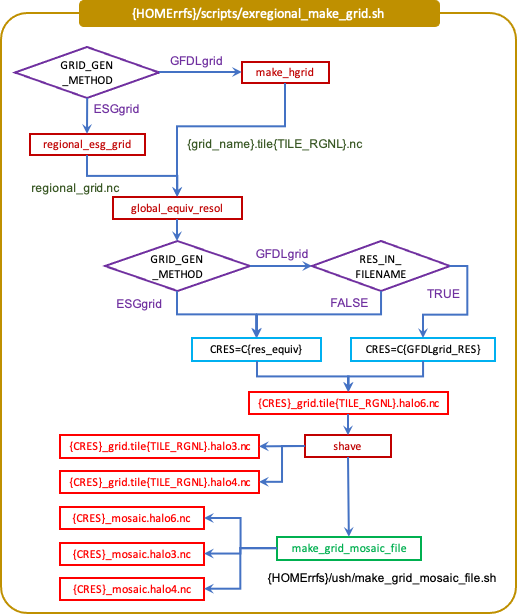
\includegraphics[width=0.6\linewidth]{FV3LAM_wflow_make_grid.png}
  \caption{Flowchart of `exregional\_make\_grid.sh' }
  \label{fig:wflow_make_grid}
\end{figure}



%---------------------------------------------------------
\subsection{Global Equivalent Resolution}
\label{subsec:global_eqv_res}

In the above flowchart, the executable `global\_equiv\_resol' calculates an equivalent global uniform cubed-sphere resolution (unit: number of cells) for the pre-defined regional grid as shown in Eq.(\ref{eq:res_equiv}). This is the `C\{res\}' that a global uniform (i.e. stretch factor of 1) cubed-sphere grid would need to have in order to have the same nominal cell size as the average cell size of the regional grid. This value is required for the topography filtering to work correctly.

\vspace{-0.3cm}

\begin{align}
\text{RES\_equiv} = \text{int} \left( \frac{2.0 \times \pi \times R_E}{4.0 \times \text{avg\_cell\_size}}  \right) 
\label{eq:res_equiv}
\end{align}
where $R_E$ is the mean radius of the earth ($\approx 6371 km$). Therefore, the `RES\_equiv' physically means the number of the average cells between the equator and  the pole along the earth's surface. For example, the global equivalent resolution of a regional grid whose average-cell-size is 2.981$km$ is C3357.



%---------------------------------------------------------
\subsection{Parameters for an ESG grid}
\label{subsec:new_predef_grid_esg}

The default values of the parameters related to an ESG grid are set in the `config\_default.sh' file as shown in Table \ref{table:config_JPgrid}. In addition, the grid-specific parameters such as those in Table \ref{table:config_configparam}, and `write-component' parameters for a new regional grid can be specified in the `set\_predef\_grid\_params.sh'.

\begin{enumerate}
\item Namelist of the ESG grid generator `regional\_grid' (`regional\_grid.nml' in `\{HOMErrfs\}/ ush/templates/'):

{
\fontsize{10}{12}\selectfont
\begin{longtable}{ p{0.1\linewidth} | p{0.74\linewidth} }
\hline
\hline
Name & Description \\
\hline
 plon & Longitude of the center of the regional domain (in degrees) \\
 plat & Latitude of the center of the regional domain (in degrees) \\
 delx & Grid spacing in the longitudinal direction on the {\it FV3} super-grid ({\bf in degrees}) \\
 & $\rightarrow$ delx $=\Delta_x / (2\times 6371)\times(180/\pi)$ where ($\Delta_x$ : $km$)  \\
 dely & Grid spacing in the latitudinal direction on the {\it FV3} super-grid ({\bf in degrees}) \\
 & $\rightarrow$ dely $=\Delta_y / (2\times 6371)\times(180/\pi)$ where ($\Delta_y$ : $km$)  \\
 lx & Negative of the number of cells in the longitudinal ($x$) direction on the super-grid from the lower-left corner to the grid center \\
& $\rightarrow$ lx$=-(\text{nx} + 2\times N_{\text{halo}})$ \\
 ly & Negative of the number of cells in the longitudinal ($y$) direction on the super-grid from the lower-left corner to the grid center \\
& $\rightarrow$ ly$=-(\text{ny} + 2\times N_{\text{halo}})$ \\
 panzi & Parameter for the starting indexes (1, 1) (0.0=SW, 180.0=NE) \\
\hline
\caption{Namelist of the the ESG (JP) grid generator.}
\label{table:namelist_esg_grid}
\end{longtable}
}

{\bf Notes)}
\begin{itemize}
\item Since the super-grid has twice the resolution of the actual grid, the grid spacing in the $x$ direction on the actual grid will be twice this resolution.
\item The physical grid spacing $\Delta_x$ on the actual grid is related to `delx' by $\Delta_x=2 \times \text{delx} \times (P_E/360)$ where $P_E$ is the Earth's circumference, and the factor 2 appears due to `delx' being the grid angle in the $x$ direction of the super-grid. Therefore, $\text{delx}=\Delta_x / (2 \times R_E ) \times (360/2\pi)$ where $R_E$ is the radius of the Earth ($\approx 6371 km$). For example, `delx=0.0135' for the 3$km$ actual grid spacing.
\item These parameters can be found by {\it fv3grid} as shown in Section \ref{subsec:fv3grid_esg_jp}.
\item The source code can be found in `$\sim$/UFS\_UTILS/sorc/grid\_tolls.fd/regional\_esg\_grid.fd'.
\end{itemize}


\item Parameters in `set\_predef\_grid\_params.sh' and `set\_gridparams\_ESGgrid.sh':

{
\fontsize{10}{12}\selectfont
\begin{longtable}{p{0.03\linewidth} | p{0.33\linewidth} | p{0.25\linewidth} | p{0.15\linewidth} }
\hline
\hline
\multirow{2}{*}{No.} & Name in `set\_predef\_  & Name in `set\_  & Name in   \\
 & grid\_params.sh' & gridparams\_ESGgrid.sh'   & Table \ref{table:namelist_esg_grid} \\
\hline
1 & ESGgrid\_LON\_CTR & lon\_ctr & plon  \\
2 & ESGgrid\_LAT\_CTR & lat\_ctr & plat  \\
3 & ESGgrid\_NX & nx & nx  \\
4 & ESGgrid\_NY & ny & ny \\
5 & ESGgrid\_DELX (in {\bf meters}) & delx (in {\bf meters}) & $\Delta_x$ \\
6 & ESGgrid\_DELY (in {\bf meters}) & dely (in {\bf meters}) & $\Delta_y$ \\
7 & ESGgrid\_WIDE\_HALO\_WIDTH & halo\_width & $N_{\text{halo}}$  \\
8 & ESGgrid\_ALPHA\_PARAM & - & a \\
9 & ESGgrid\_KAPPA\_PARAM & - & k \\
10 & - & stretch\_factor & - \\
11 & - & del\_angle\_x\_sg & delx  \\
12 & - & del\_angle\_y\_sg & dely  \\
13 & - & neg\_nx\_of\_dom\_with\_ wide\_halo & lx  \\
14 & - & neg\_ny\_of\_dom\_with\_ wide\_halo & ly  \\
\hline
\caption{Grid parameters for an ESG (JP) grid.}
\label{table:gridparams_jp}
\end{longtable}
}

{\bf Notes)}
\begin{itemize}
\item Make sure that `ESGgrid\_DELX' and `ESGgrid\_DELY' are in meters because the `radius\_Earth' ($R_E$ in Table \ref{table:namelist_esg_grid} ) is set in meters in `constants.sh'.
\item The variable names of `delx' and `dely' means totally different parameters between `set\_ gridparams\_ESGgrid.sh' and the namelist of `regional\_grid'. The grid spacing parameters `delx' and `dely' in degrees are calculated in `set\_gridparams\_ESGgrid.sh' based on the input parameters `delx' and `dely' in meters of `set\_predef\_grid\_params.sh'. 
\item If any `ESGgrid\_XXX' parameters are not specified in `set\_predef\_grid\_params.sh', the default values in `config\_defaults.sh' or the pre-defined values in `config.sh' will be used. 
\end{itemize}

\end{enumerate}


%---------------------------------------------------------
\subsection{Parameters for a GFDL grid}
\label{subsec:new_predef_grid_gfdl}

The default values of the parameters related to a GFDL grid are set in the `config\_default.sh' file as shown in Table \ref{table:config_GFDLgrid}. In addition, the grid-specific parameters such as those in Table \ref{table:config_configparam}, and `write-component' parameters can be specified in the `set\_predef\_grid\_params.sh'.

\begin{enumerate}
\item Namelist of the GFDL grid generator `make\_hgrid' (shown in `\{HOMErrfs\}/scripts/exregional \_make\_grid.sh'):

{
\fontsize{10}{12}\selectfont
\begin{longtable}{p{0.15\linewidth} | p{0.75\linewidth} }
\hline
\hline
 Parameter name & Description \\
\hline
 grid\_type & Type of topography (=`gnomonic\_ed': equal distance gnomonic cubic grid) \\
 nlon & Number of model grid points (super-grid) for each zonal regions of varying resolution (2$\times$\{res\}) \\
 grid\_name & Name of output grid (=C\{res\}\_grid) \\
 do\_schmidt & Set to do Schmidt transformation to create stretched grid \\
 stretch\_factor & Stretching factor for the grid \\
 target\_lon & Center longitude of the regional domain (tile 7) \\
 target\_lat & Center latitude of the regional domain (tile 7) \\
 nest\_grid &  Option for a regional grid\\
 parent\_tile & Parent tile number of a regional grid (=6)\\
 refine\_ratio & Grid refinement ratio for a regional grid \\
 istart\_nest & Starting $i$-directional index of a regional grid on the parent tile super-grid (Fortran index) \\
 jstart\_nest & Ending $i$-directional index of a regional grid on the parent tile super-grid (Fortran index) \\
 iend\_nest & Starting $j$-directional index of a regional grid on the parent tile super-grid (Fortran index) \\
 jend\_nest & Ending $j$-directional index of a regional grid on the parent tile super-grid (Fortran index) \\
 halo & Lateral boundary halo size (only for a regional grid) \\
 great\_circle\_ algorithm & When specified, the `greate\_circle\_algorithm' will be used to compute grid cell areas \\
\hline
\caption{Namelist of the the GFDL grid generator.}
\label{table:namelist_gfdl_grid}
\end{longtable}
}

\item Parameters in `set\_predef\_grid\_params.sh' and `set\_gridparams\_GFDLgrid.sh':

{
\fontsize{10}{12}\selectfont
\begin{longtable}{p{0.03\linewidth} | p{0.31\linewidth} | p{0.31\linewidth} | p{0.15\linewidth} }
\hline
\hline
\multirow{2}{*}{No.} & Name in `set\_predef\_  & Name in `set\_gridparams\_  & Name in   \\
 & grid\_params.sh' & GFDLgrid.sh'   & Table \ref{table:namelist_gfdl_grid}\\
\hline
1 & GFDLgrid\_LON\_T6\_CTR & lon\_of\_t7\_ctr  & target\_lon  \\
2 & GFDLgrid\_LAT\_T6\_CTR & lat\_of\_t7\_ctr & target\_lat \\
3 & GFDLgrid\_STRETCH\_FAC & stretch\_factor & stretch\_factor \\
4 & GFDLgrid\_RES & res\_of\_t6g & - \\
5 & GFDLgrid\_REFINE\_RATIO & refine\_ratio\_t6g\_to\_t7g & refine\_ratio \\
6 & GFDLgrid\_ISTART\_OF\_ RGNL\_DOM\_ON\_T6G & istart\_of\_t7\_on\_t6g & - \\
7 & GFDLgrid\_IEND\_OF\_RGNL\_ DOM\_ON\_T6G & iend\_of\_t7\_on\_t6g & - \\
8 & GFDLgrid\_JSTART\_OF\_ RGNL\_DOM\_ON\_T6G & jstart\_of\_t7\_on\_t6g & - \\
9 & GFDLgrid\_JEND\_OF\_RGNL\_ DOM\_ON\_T6G & jend\_of\_t7\_on\_t6g & - \\
10 & GFDLgrid\_USE\_GFDLgrid\_ RES\_IN\_FILENAMES & jend\_of\_t7\_on\_t6g & - \\
11 & - & nx\_of\_t7\_on\_t7g & - \\
12 & - & ny\_of\_t7\_on\_t7g & - \\
13 & - & halo\_width\_on\_t7g & - \\
14 & - & istart\_of\_t7\_with\_halo\_on\_t6sg & istart\_nest \\
15 & - & iend\_of\_t7\_with\_halo\_on\_t6sg & iend\_nest \\
16 & - & jstart\_of\_t7\_with\_halo\_on\_t6sg & jstart\_nest \\
17 & - & jend\_of\_t7\_with\_halo\_on\_t6sg & jend\_nest \\
\hline
\caption{Grid parameters for a GFDL grid.}
\label{table:gridparams_gfdl}
\end{longtable}
}

{\bf Notes)}
\begin{itemize}
\item The index numbers of 5--9 in Table \ref{table:gridparams_gfdl} are {\bf NOT} those on the super-grid but they are the numbers on a general grid such as orography. Therefore, if you use `fv3grid' to set up the size of a new regional domain, you should divide the numbers on `fv3grid' by 2. 
\item In the scripts for the GFDL grid-generation, `GFDLgrid\_RES' is used to set the number of cells along the longitudinal/latitudinal direction on a general grid (not super-grid). For example, `GFDLgrid\_RES' = 768 in the `C768' grid system. The number of cells along the longitudinal (latitudianl) direction on the super-grid is $2\times768$.  
\end{itemize}
 

The GFDL gird generation executable `make\_hgrid' requires the index limits such as starting and ending indices of the regional grid on the super-grid of its {\bf parent} tile (Tile 6). The index limits on the super-grid of the parent tile are represented as
\lstset{language=bash}   
\begin{lstlisting}[frame=trBL,mathescape=true]
istart_of_t7_on_t6sg = 2 $\times$ istart_of_t7_on_t6g -1 
iend_of_t7_on_t6sg = 2 $\times$ iend_of_t7_on_t6g  
jstart_of_t7_on_t6sg = 2 $\times$ jstart_of_t7_on_t6g -1 
jend_of_t7_on_t6sg = 2 $\times$ jend_of_t7_on_t6g  
\end{lstlisting}
where `t6sg' denotes the super-grid of Tile 6, and `t6g' means the normal grid of Tile 6. \\

To obtain a regional grid with a halo, the index limits must include the halo number. The starting indices on the super-grid of Tile 6 with wide halo must be odd while the ending indices must be even. We subtract 1 from the starting indices if they are even (which ensures that there will be at least `halo\_width\_on\_t7g' halo cells along the left and bottom boundaries), and we add 1 to the ending indices if they are odd for the right and top boundaries:

\lstset{language=bash}   
\begin{lstlisting}[frame=trBL,mathescape=true, basicstyle=\small]
istart_of_t7_with_halo_on_t6sg = istart_of_t7_on_t6g - halo_width_on_t6sg (-1, if even) 
iend_of_t7_with_halo_on_t6sg = iend_of_t7_on_t6g + halo_width_on_t6sg (+1, if odd) 
jstart_of_t7_with_halo_on_t6sg = jstart_of_t7_on_t6g - halo_width_on_t6sg (-1, if even)
jend_of_t7_with_halo_on_t6sg = jend_of_t7_on_t6g + halo_width_on_t6sg  (+1, if odd)
\end{lstlisting}
where
\lstset{language=bash}   
\begin{lstlisting}[frame=trBL,mathescape=true, basicstyle=\small]
halo_width_on_t6sg={2$\times (\{NH4=4\}+1)$+ refine_ratio_t6g_to_t7g -1}/refine_ratio_t6g_to_t7g
\end{lstlisting}
\vspace{0.5cm}

To calculate the number of cells along the longitudinal ($x$) and latitudinal ($y$) directions in the regional domain:
\lstset{language=bash}   
\begin{lstlisting}[frame=trBL,mathescape=true, basicstyle=\small]
nx_of_t7_on_t7g={(iend_of_t7_on_t6sg-istart_of_t7_on_t6sg+1)/2}$\times$refine_ratio_t6g_to_t7g
ny_of_t7_on_t7g={(jend_of_t7_on_t6sg-jstart_of_t7_on_t6sg+1)/2}$\times$refine_ratio_t6g_to_t7g
\end{lstlisting}

\vspace{0.5cm}
{\bf Note)} There are two different ways to create a regional grid as shown in Table \ref{table:namelist_gfdl_grid_2ways}. One is to set the indices of 11 to 14 in Table \ref{table:namelist_gfdl_grid} to be the same as the exact regional domain and set `halo' to 3 as shown in Sections \ref{sec:sar_pre_grid} and \ref{sec:dev_sar_grid} (`without workflow'). The other is to include the adjusted halo number (`halo\_width\_on\_t6sg') in the indices of 11 to 14 and set `halo' to 1 as described in this section (`with workflow'). However, in either case, the three different domains with halo0, halo3, and halo4 will be created by the executable `shave.x' later.
{
\fontsize{10}{12}\selectfont
\begin{longtable}{ p{0.18\linewidth} | p{0.25\linewidth} | p{0.32\linewidth} }
\hline
\hline
 Namelist parameter & Case 1 (w/o workflow) & Case 2 (w/ workflow) \\
\hline
 istart\_nest & istart\_of\_t7\_on\_t6g &istart\_of\_t7\_with\_halo\_on\_t6sg \\
 iend\_nest & iend\_of\_t7\_on\_t6g & iend\_of\_t7\_with\_halo\_on\_t6sg\\
 jstart\_nest & jstart\_of\_t7\_on\_t6g & jstart\_of\_t7\_with\_halo\_on\_t6sg \\
 jend\_nest & jend\_of\_t7\_on\_t6g & jend\_of\_t7\_with\_halo\_on\_t6sg\\
 halo & 3 & 1 \\
\hline
\caption{Two different approaches to create a GFDL grid.}
\label{table:namelist_gfdl_grid_2ways}
\end{longtable}
}

\end{enumerate}



%---------------------------------------------------------
\subsection{Running a Workflow for a New Grid with an Example}
\label{subsec:new_predef_grid_wflow}

\begin{enumerate}
\item Get the parameters for a new grid from {\it fv3grid} as describe in Section \ref{sec:post_grid}: 

\begin{itemize}
\item ESG grid parameters:

{\bf Note)} To match the parameters of {\it fv3grid} with those of the script, make sure that $\text{lx}\times-2=\text{nx}$ and $\text{ly}\times-2=\text{ny}$.

{
\fontsize{10}{12}\selectfont
\begin{longtable}{p{0.15\linewidth} | p{0.1\linewidth} | p{0.4\linewidth}  }
\hline
\hline
 Parameter & Value & Name in the script \\
\hline
 plon & -75.0 & ESGgrid\_LON\_CTR \\
 plat & 28.5 & ESGgrid\_LAT\_CTR \\
 delx & 0.0135 & (=3000 for `ESGgrid\_DELX') \\
 dely & 0.0135 & (=3000 for `ESGgrid\_DELX') \\
 lx & -1500 &  -(ESGgrid\_NX) \\
 ly & -1200 & -(ESGgrid\_NY) \\
 nx & 3000 & $2\times$ESGgrid\_NX \\
 ny & 2400 & $2\times$ESGgrid\_NY \\
\hline
\caption{Parameters for ESG grid}
\label{table:var_ecoast_esg}
\end{longtable}
}

\begin{figure}[ht!]
  \centering
  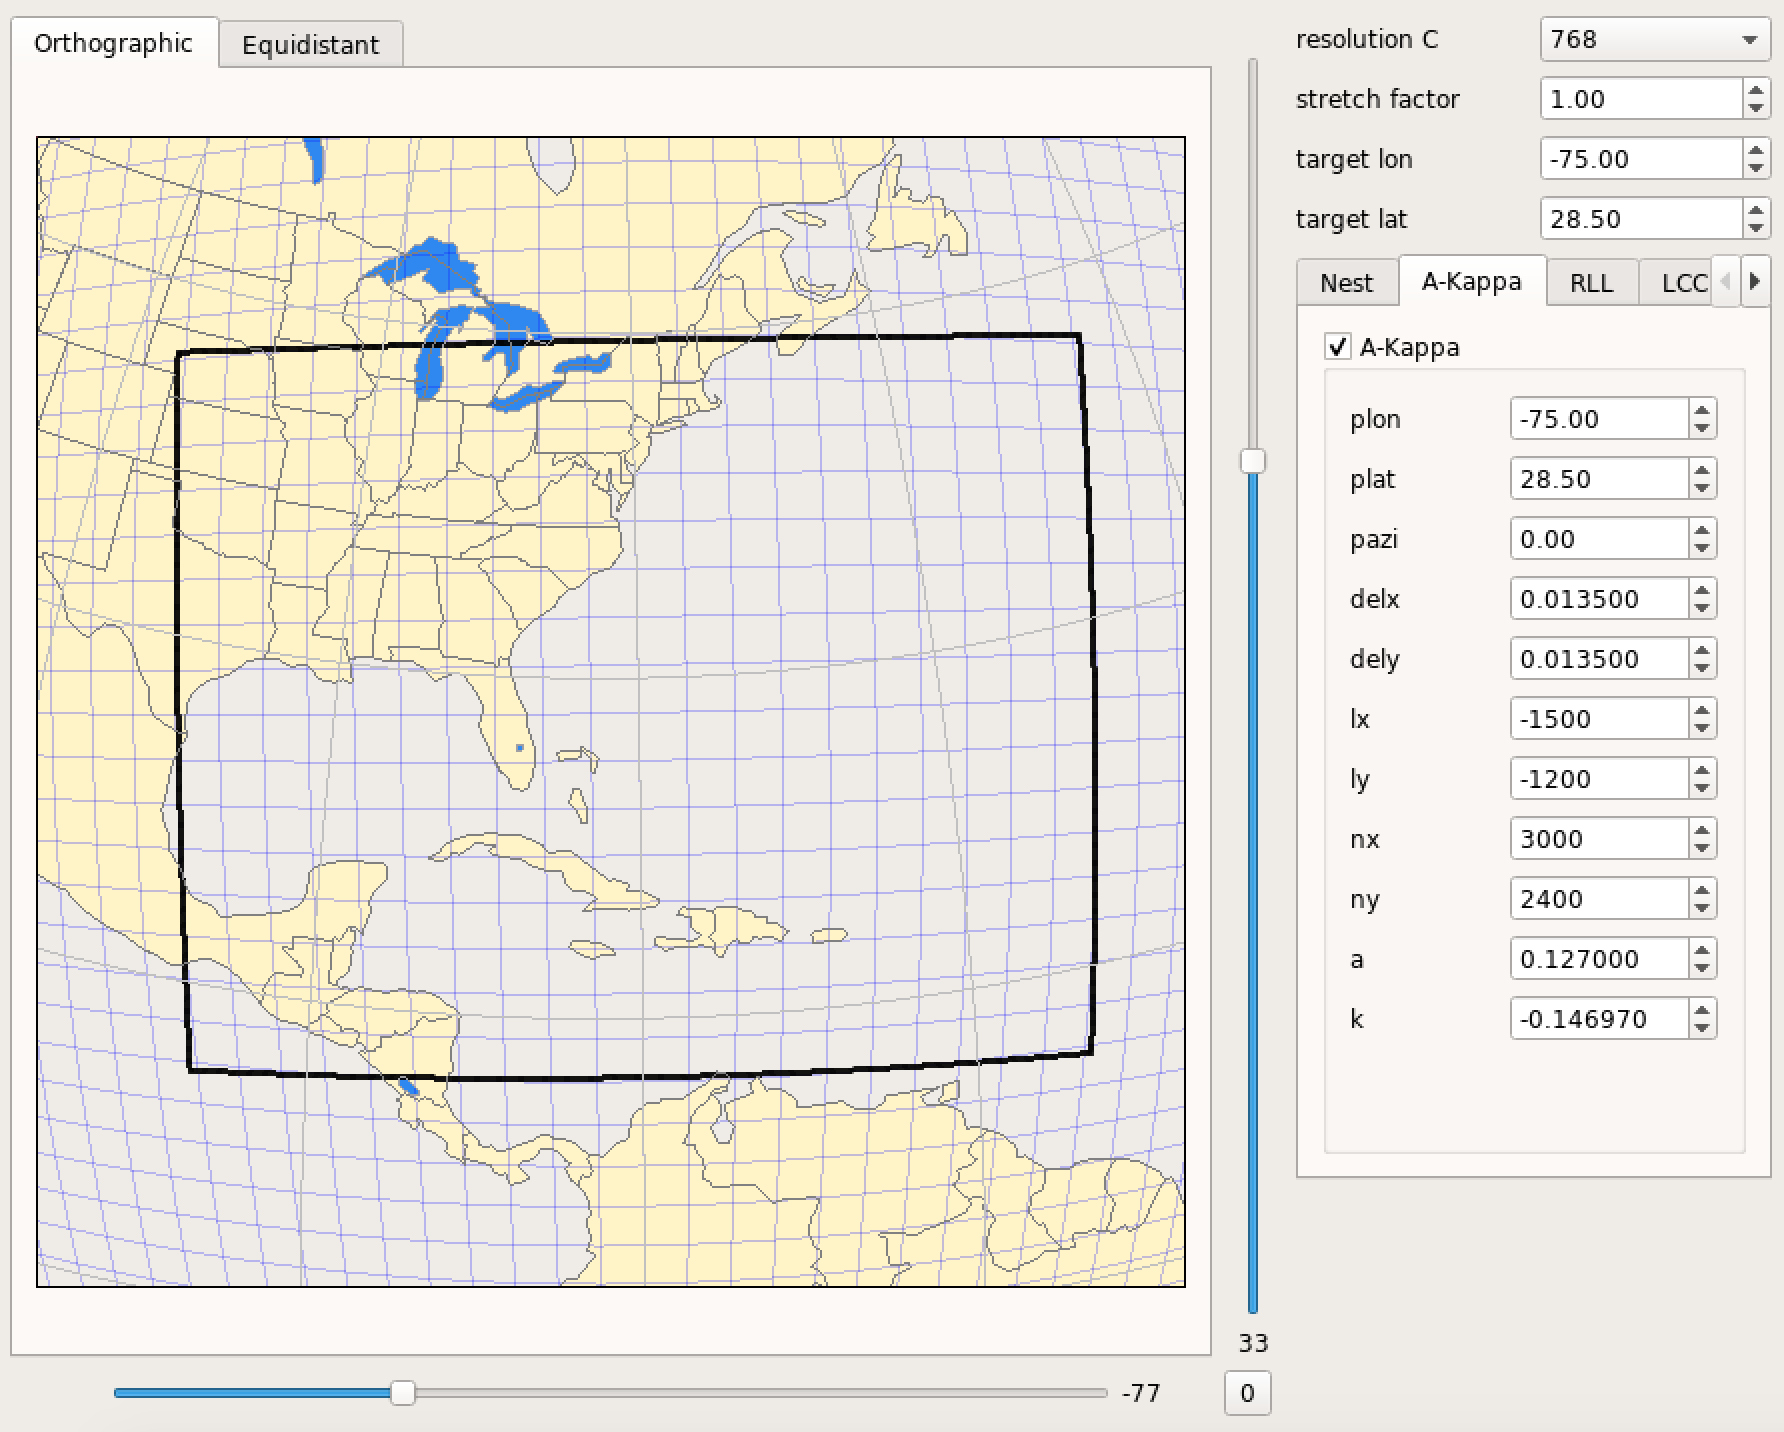
\includegraphics[width=0.7\linewidth]{ECoast_JCH_esg.png}
  \caption{ESG grid parameters for the East Coast domain by {\it fv3grid} }
  \label{fig:fv3grid_ecoast_esg}
\end{figure}


\item GFDL grid parameters:

\begin{itemize}
\item Since we supposed that the center of the regional domain is located at the center of the parent tile (Tile 6), we recommend to make the domain symmetry by setting `I end'=$2\times$`resolution C'-(`I start'-1) and `J end'=$2\times$`resolution C'-(`J start'-1).
\item You can use `num\_margin\_cells\_T6\_[left/right/bottom/top]' to make a symmetry domain along the centerline of the parent tile 6.
\item The starting and ending indices (7--10 in Table \ref{table:var_ecoast_gfdl}) should be adjusted in `set\_ gridparams\_GFDLgrid.sh' to satisfy the HPC environment configuration shown in Section \ref{sec:config_hpc}.
\end{itemize}

{
\fontsize{10}{12}\selectfont
\begin{longtable}{ p{0.15\linewidth} | p{0.1\linewidth} | p{0.6\linewidth}  }
\hline
\hline
 Parameter & Value & Name in the script \\
\hline
 resolution C & 768 & GFDLgrid\_RES \\
 stretch factor & 1.50 & GFDLgrid\_STRETCH\_FAC  \\
 target lon & -75.0 & GFDLgrid\_LON\_T6\_CTR \\ 
 target lat & 28.5 & GFDLgrid\_LAT\_T6\_CTR \\
 parent & 6 & - \\
 refine ratio & 3 & GFDLgrid\_REFINE\_RATIO \\
 I start & 261 & $\approx 2\times$GFDLgrid\_ISTART\_OF\_RGNL\_DOM\_ON\_T6G \\
 J start & 361 & $\approx 2\times$GFDLgrid\_JSTART\_OF\_RGNL\_DOM\_ON\_T6G \\
 I end & 1280 & $\approx 2\times$GFDLgrid\_IEND\_OF\_RGNL\_DOM\_ON\_T6G \\
 J end & 1160 & $\approx 2\times$GFDLgrid\_JEND\_OF\_RGNL\_DOM\_ON\_T6G \\
\hline
\caption{Parameters for GFDL grid}
\label{table:var_ecoast_gfdl}
\end{longtable}
}

\begin{figure}[ht!]
  \centering
  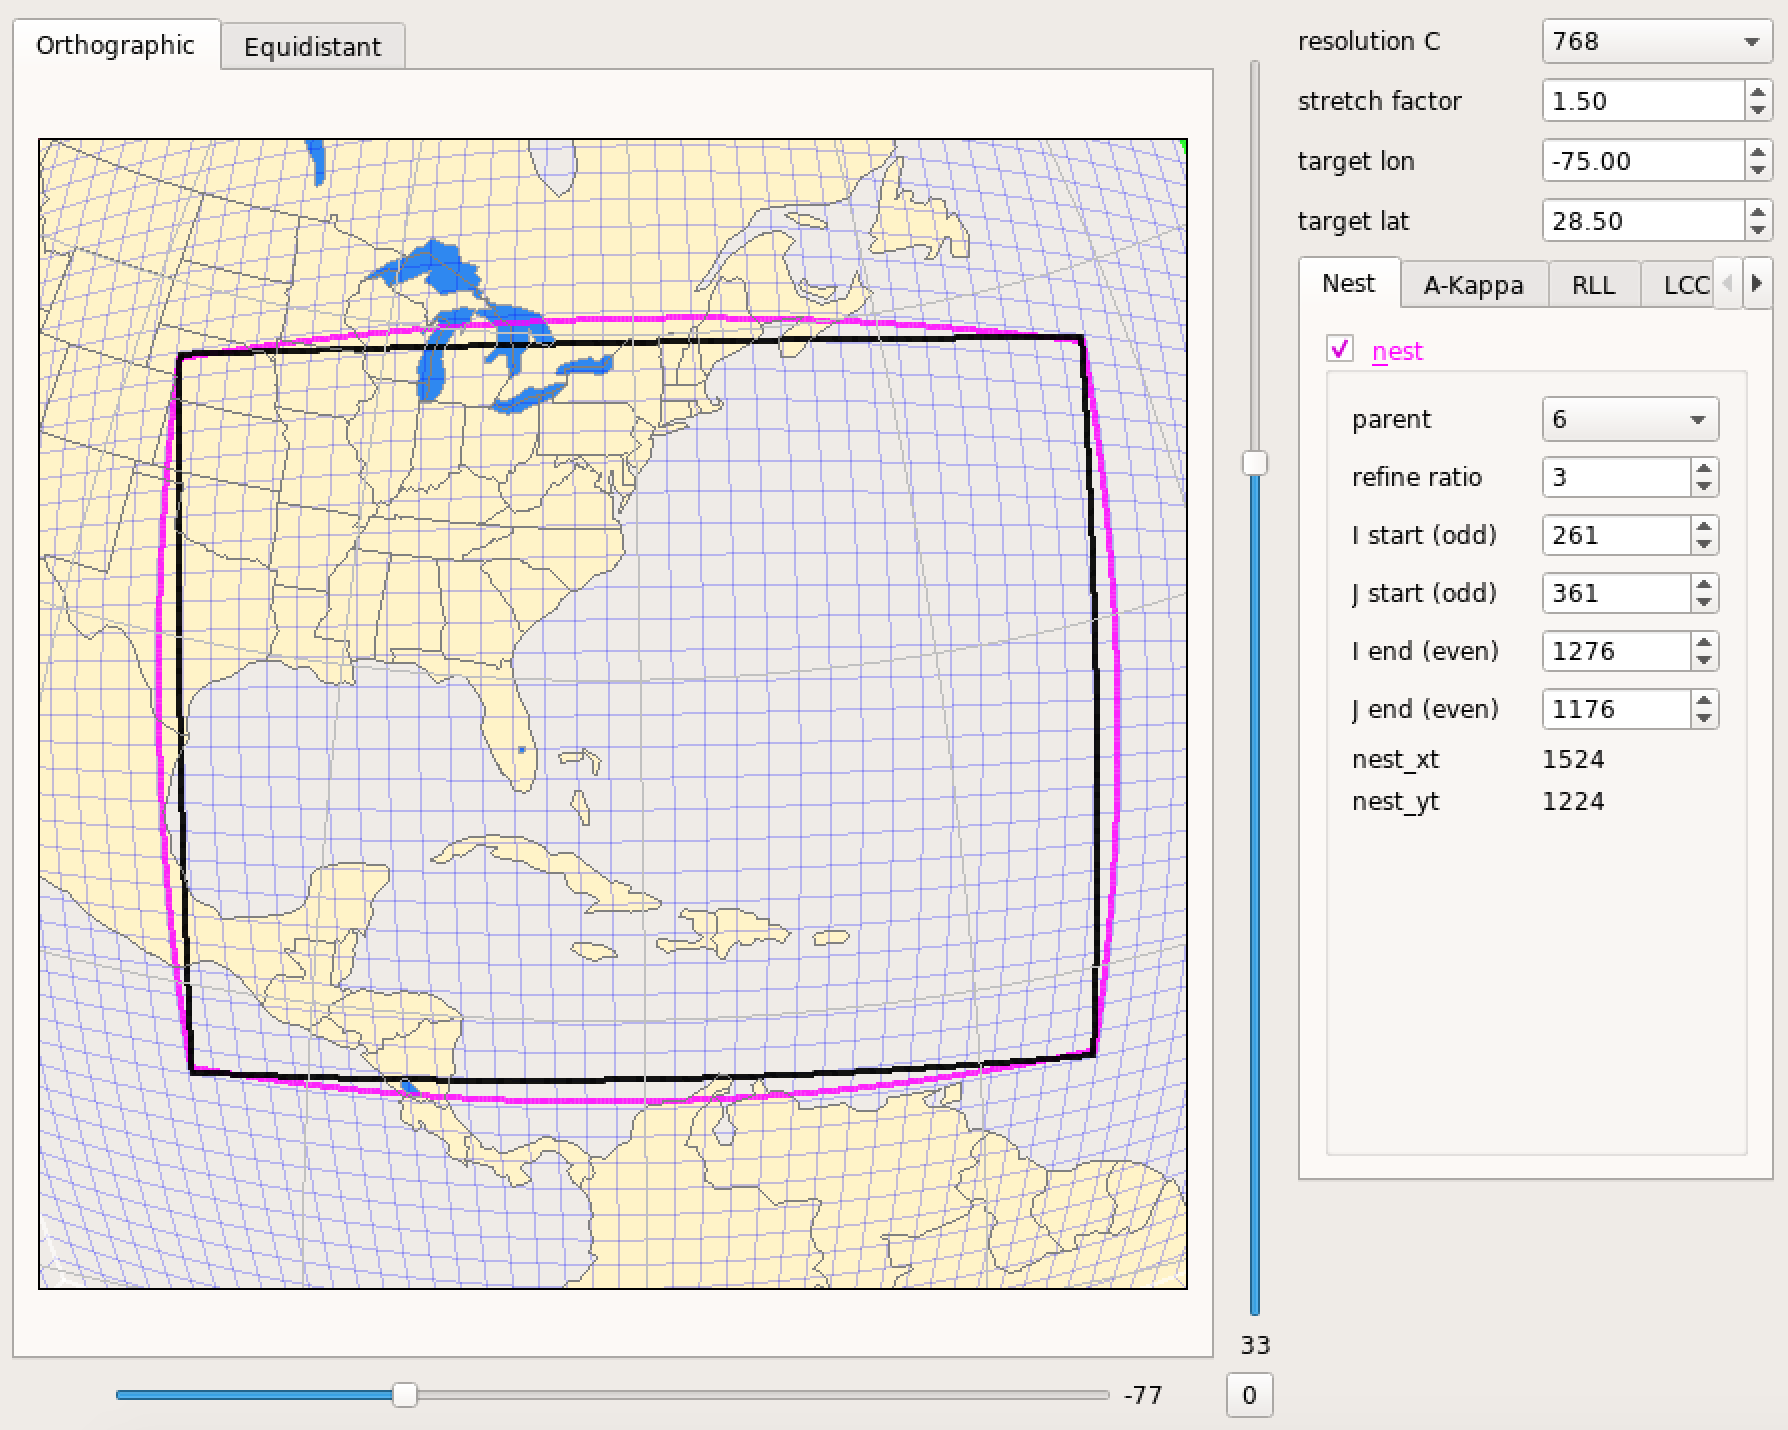
\includegraphics[width=0.69\linewidth]{ECoast_JCH_gfdl.png}
  \caption{GFDL grid parameters for the East Coast domain by {\it fv3grid} }
  \label{fig:fv3grid_ecoast_gfdl}
\end{figure}


\item Rotated Lat-Lon (RLL) parameters (for `QUILTING'=`TRUE'):
\begin{figure}[ht!]
  \centering
  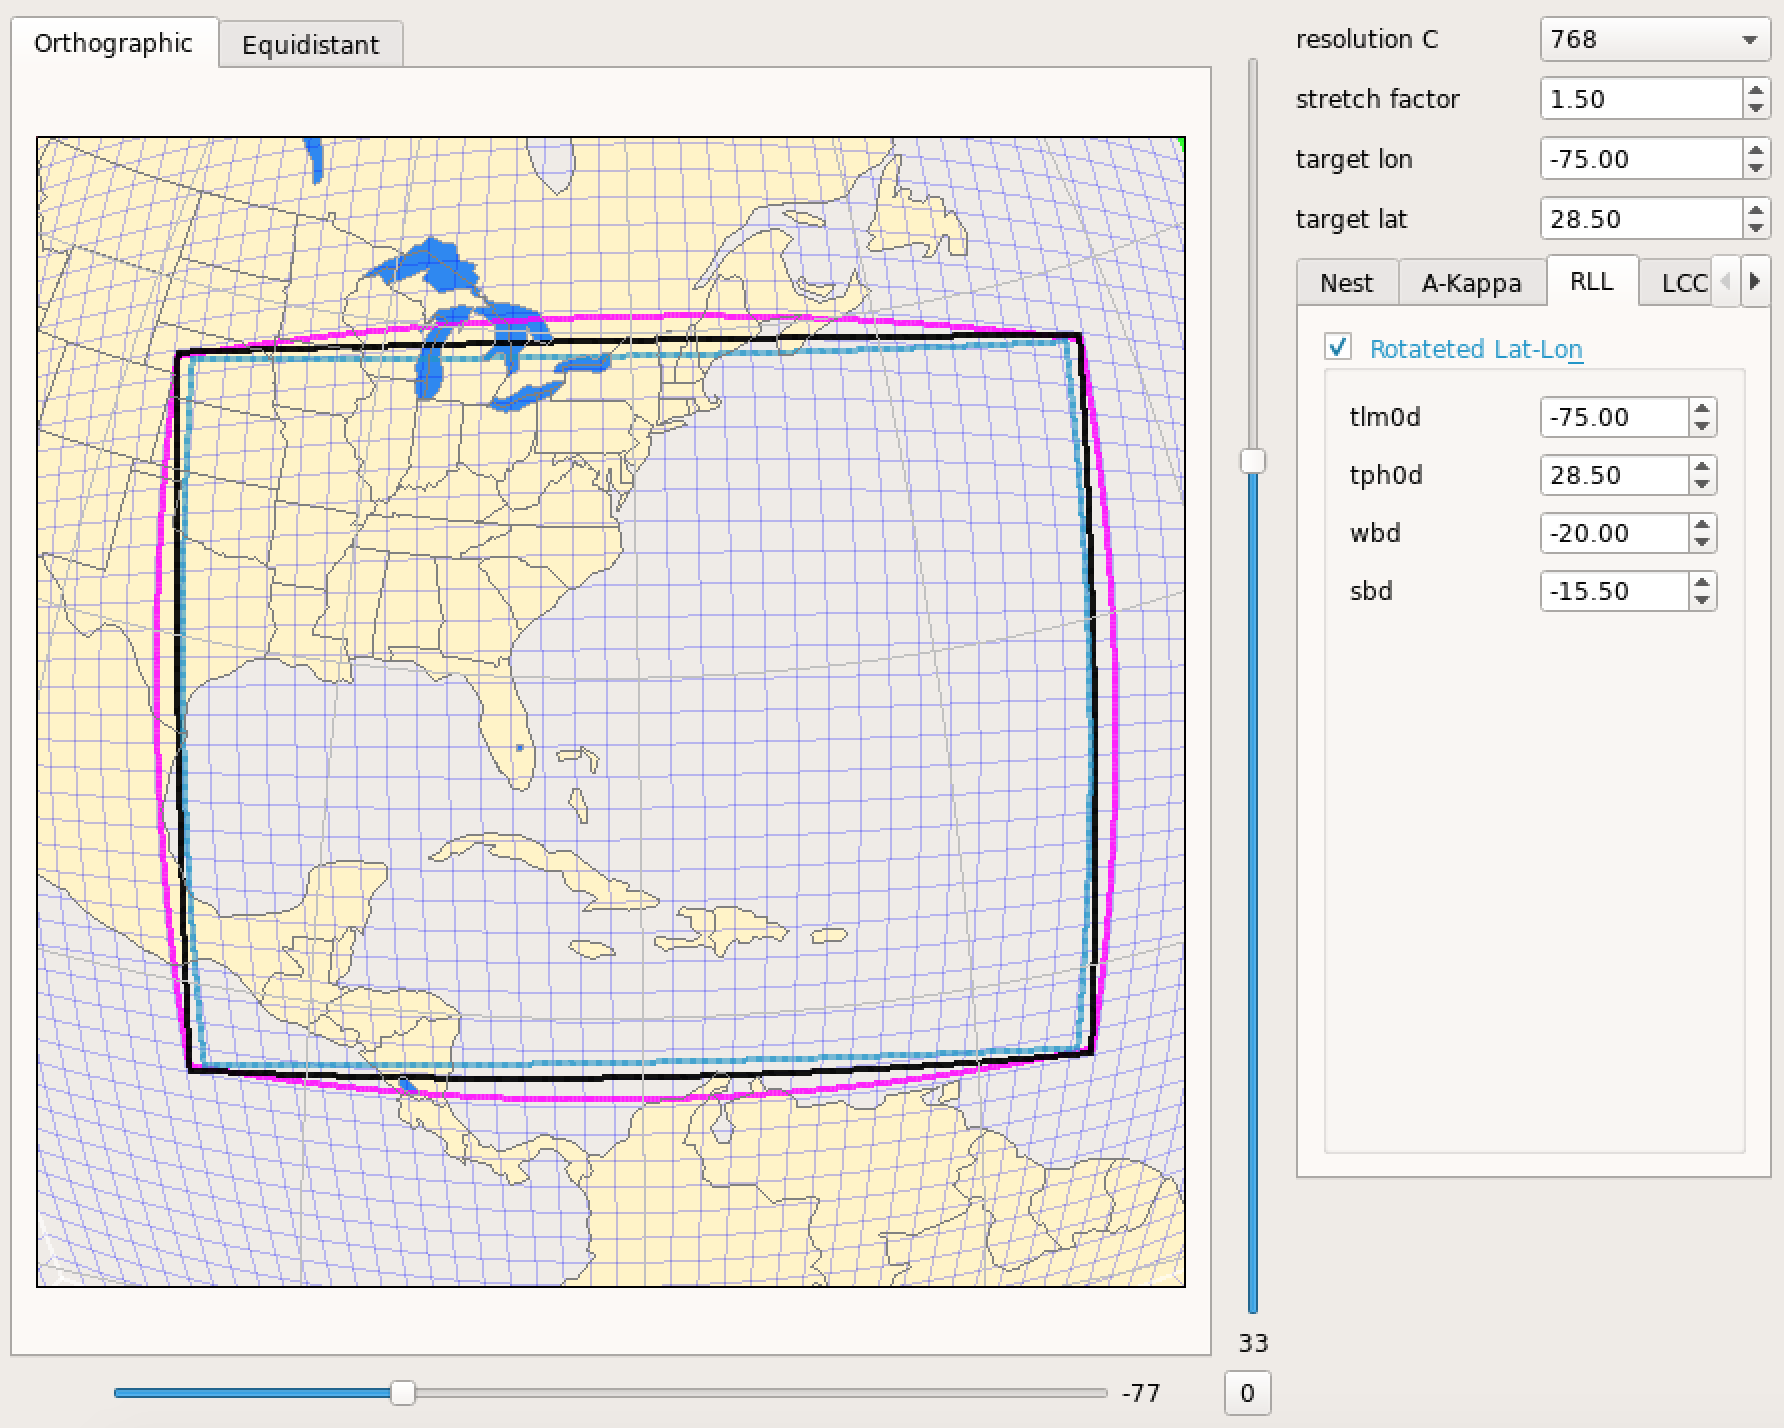
\includegraphics[width=0.69\linewidth]{ECoast_JCH_rll.png}
  \caption{Write-component parameters for the East Coast domain by {\it fv3grid} }
  \label{fig:fv3grid_ecoast_rll}
\end{figure}

{
\fontsize{10}{12}\selectfont
\begin{longtable}{p{0.03\linewidth} | p{0.15\linewidth} | p{0.1\linewidth} | p{0.55\linewidth}  }
\hline
\hline
No. & Parameter & Value & Name in the script \\
\hline
1 & tlm0d & -75.0 & WRTCMP\_cen\_lon  \\
2 & tph0d & 28.5 & WRTCMP\_cen\_lat \\
3 & wbd & -20.0 & WRTCMP\_lon\_lwr\_left \\
4 & sbd & -15.5 & WRTCMP\_lat\_lwr\_left \\
\hline
\caption{Parameters for the write component of the GFDL grid}
\label{table:var_ecoast_wrtcmp}
\end{longtable}
}


\end{itemize}

\item Add the name of the new grid to the list defined by `valid\_vals\_PREDEF\_GRID\_NAME':
\lstset{language=bash}   
\begin{lstlisting}[frame=trBL]
cd {HOMErrfs}/ush/
vim valid_param_vals.sh
(add) ``JCH_ECOAST_3km'' \
\end{lstlisting}

\item Add the new grid to the list of grids in the case statement of `\{PREDEF\_GRID\_NAME\}':
\lstset{language=bash}   
\begin{lstlisting}[frame=trBL]
cd {HOMErrfs}/ush/
vim set_predef_grid_params.sh
\end{lstlisting}

Add below:
\lstset{language=bash}   
\begin{lstlisting}[frame=trBL, basicstyle=\tiny]
#---------------------------------------
# Test grid for East Coast by Chan-Hoo Jeon
#--------------------------------------
#
"JCH_ECOAST_3km")
  if [ "${GRID_GEN_METHOD}" = "GFDLgrid" ]; then
    GFDLgrid_LON_T6_CTR=-75.0
    GFDLgrid_LAT_T6_CTR=28.5
    GFDLgrid_STRETCH_FAC=1.5
    GFDLgrid_RES="768"
    GFDLgrid_REFINE_RATIO=3
  
    num_margin_cells_T6_left=120
    GFDLgrid_ISTART_OF_RGNL_DOM_ON_T6G=$(( num_margin_cells_T6_left + 1 ))
    num_margin_cells_T6_right=120
    GFDLgrid_IEND_OF_RGNL_DOM_ON_T6G=$(( GFDLgrid_RES - num_margin_cells_T6_right ))
    num_margin_cells_T6_bottom=180
    GFDLgrid_JSTART_OF_RGNL_DOM_ON_T6G=$(( num_margin_cells_T6_bottom + 1 ))
    num_margin_cells_T6_top=180
    GFDLgrid_JEND_OF_RGNL_DOM_ON_T6G=$(( GFDLgrid_RES - num_margin_cells_T6_top ))
    GFDLgrid_USE_GFDLgrid_RES_IN_FILENAMES="TRUE"

    DT_ATMOS="18"
    LAYOUT_X="24"
    LAYOUT_Y="24"
    BLOCKSIZE=18

    if [ "$QUILTING" = "TRUE" ]; then
      WRTCMP_write_groups="1"
      WRTCMP_write_tasks_per_group=$(( 1*LAYOUT_Y ))
      WRTCMP_output_grid="rotated_latlon"
      WRTCMP_cen_lon="-75.0"
      WRTCMP_cen_lat="28.5"
      WRTCMP_lon_lwr_left="-20.0"
      WRTCMP_lat_lwr_left="-15.5"
      WRTCMP_lon_upr_rght="20.0"
      WRTCMP_lat_upr_rght="15.5"
      WRTCMP_dlon="0.02"
      WRTCMP_dlat="0.02"
    fi
  elif [ "${GRID_GEN_METHOD}" = "ESGgrid" ]; then
    ESGgrid_LON_CTR=-75.0
    ESGgrid_LAT_CTR=28.5
    ESGgrid_DELX="3000.0"
    ESGgrid_DELY="3000.0"
    ESGgrid_NX=1500
    ESGgrid_NY=1200
    ESGgrid_WIDE_HALO_WIDTH=6
    
    DT_ATMOS="18"
    LAYOUT_X="30"
    LAYOUT_Y="40"
    BLOCKSIZE=30

    if [ "$QUILTING" = "TRUE" ]; then
      WRTCMP_write_groups="1"
      WRTCMP_write_tasks_per_group=$(( 1*LAYOUT_Y ))
      WRTCMP_output_grid="rotated_latlon"
      WRTCMP_cen_lon="-75.0"
      WRTCMP_cen_lat="28.5"
      WRTCMP_lon_lwr_left="-20.0"
      WRTCMP_lat_lwr_left="-15.5"
      WRTCMP_lon_upr_rght="20.0"
      WRTCMP_lat_upr_rght="15.5"
      WRTCMP_dlon="0.02"
      WRTCMP_dlat="0.02"
    fi    
  fi
  ;;
#

\end{lstlisting}

\item Edit `config.community.sh'.

\lstset{language=bash}   
\begin{lstlisting}[frame=trBL]
cd {HOMErrfs}/ush/
vim config.community.sh
\end{lstlisting}


\begin{itemize}
\item ESG (JP) grid:

\lstset{language=bash}   
\begin{lstlisting}[frame=trBL, basicstyle=\small]
EXPT_SUBDIR="jch_ecoast_esg"
RUN_ENVIR="community"
PREDEF_GRID_NAME="JCH_ECOAST_3km"
GRID_GEN_METHOD="ESGgrid"
RUN_TASK_MAKE_GRID="TRUE"
RUN_TASK_MAKE_OROG="TRUE"
RUN_TASK_MAKE_SFC_CLIMO="TRUE"
\end{lstlisting}

{\bf Note)} Unless the pre-generated surface climatology files exist, `RUN\_TASK\_MAKE\_ SFC\_CLIMO' should be set to ``TRUE''.

\item GFDL grid:

\lstset{language=bash}   
\begin{lstlisting}[frame=trBL, basicstyle=\small]
EXPT_SUBDIR="jch_ecoast_gfdl"
RUN_ENVIR="community"
PREDEF_GRID_NAME="JCH_ECOAST_3km"
GRID_GEN_METHOD="GFDLgrid"
RUN_TASK_MAKE_GRID="TRUE"
RUN_TASK_MAKE_OROG="TRUE"
RUN_TASK_MAKE_SFC_CLIMO="TRUE"
\end{lstlisting}


\end{itemize}

\item Load the machine-specific modules on HPC:

\begin{itemize}
\item On Hera:
\lstset{language=bash}   
\begin{lstlisting}[frame=trBL]
module use -a /contrib/miniconda3/modulefiles
module load miniconda3
conda activate regional_workflow
\end{lstlisting}
\end{itemize}

\item Generate a workflow:

\lstset{language=bash}   
\begin{lstlisting}[frame=trBL]
cd {HOMErrfs}/ush/
cp config.community.sh config.sh
./generate_FV3LAM_wflow.sh
\end{lstlisting}

\item Run the workflow:

\lstset{language=bash}   
\begin{lstlisting}[frame=trBL]
cd {EXPTDIR}
./launch_FV3LAM_wflow.sh
tail -n 30 log.launch_FV3LAM_wflow
\end{lstlisting}

\item The grid and mosaic files should be found in:

\lstset{language=bash}   
\begin{lstlisting}[frame=trBL]
cd {EXPTDIR}/grid/
\end{lstlisting}

{\bf Note)} Once the orography files are obtained from Section \ref{sec:sar_wflow_oro}, the grid and orography files can be plotted by the supporting tool shown in Section \ref{subsec:python_grid_oro}.


\begin{figure}[ht!]
  \centering
  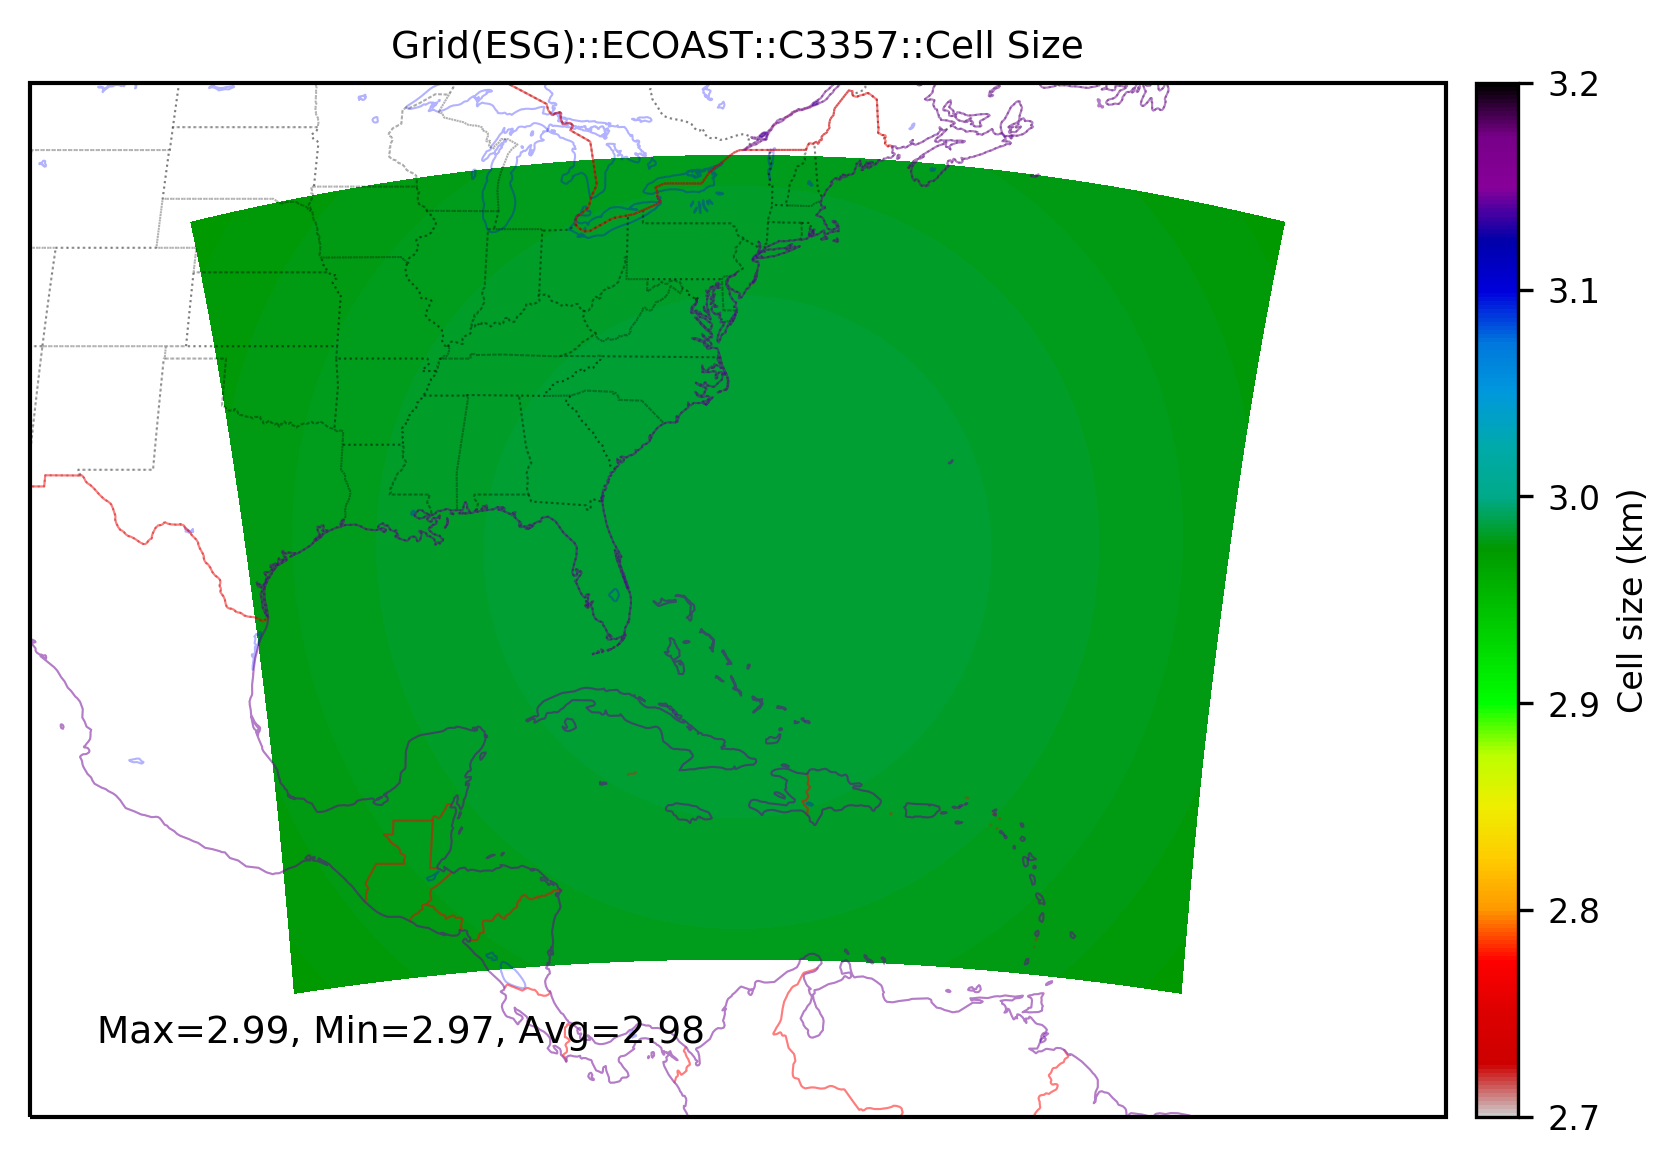
\includegraphics[width=0.49\linewidth]{fv3_grid_only_ECOAST_esg_C3357_dxy.png}
  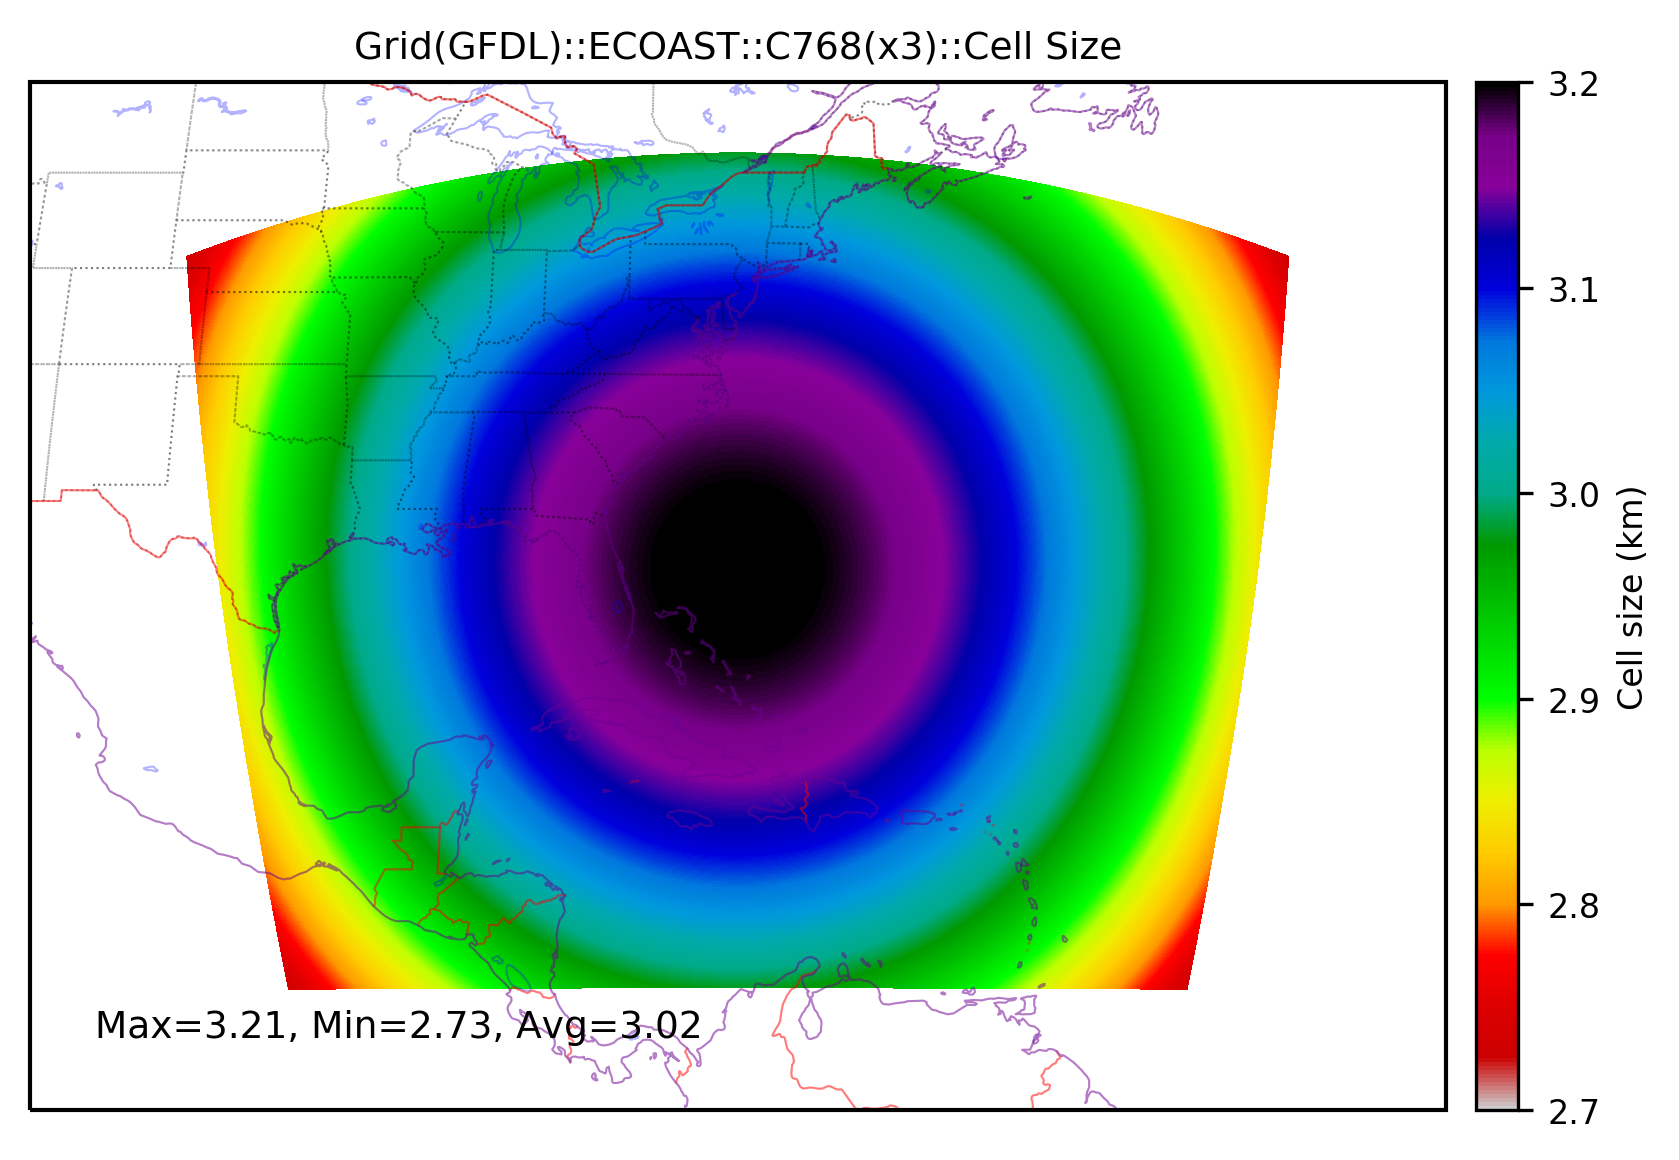
\includegraphics[width=0.49\linewidth]{fv3_grid_only_ECOAST_gfdl_C768_dxy.png}
  \caption{Comparison of cell sizes between ESG and GFDL }
  \label{fig:comp_grid_esg_gfdl}
\end{figure}

\end{enumerate}



%=================================================== 
\section{Orography}
\label{sec:sar_wflow_oro}

Once the grid-generation task described in Section \ref{sec:sar_wflow_grd_esg_gfdl} is complete, the orography files can be obtained by running the regional workflow again: 

\lstset{language=bash}   
\begin{lstlisting}[frame=trBL]
cd {EXPTDIR}
./launch_FV3LAM_wflow.sh
tail -n 30 log.launch_FV3LAM_wflow
\end{lstlisting}

\vspace{0.3cm}

The flowchart of orography generation is shown in Figure \ref{fig:wflow_make_orog}. The list of executables used for the orography-generation job is as follows:
\begin{enumerate}
\item orog
\item filter\_topo
\item shave
\end{enumerate}


\begin{figure}[ht!]
  \centering
  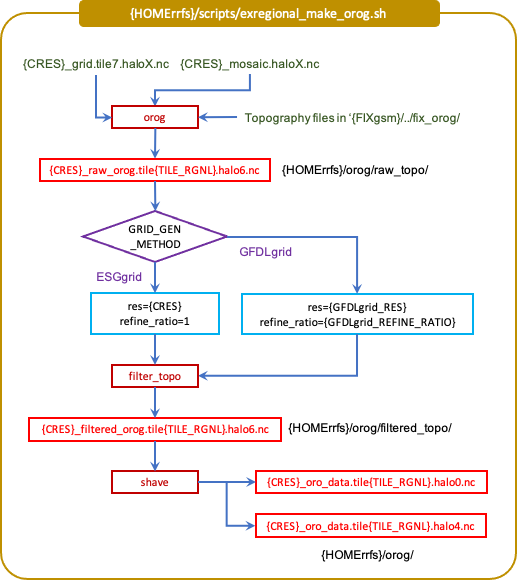
\includegraphics[width=0.6\linewidth]{FV3LAM_wflow_make_orog.png}
  \caption{Flowchart of `exregional\_make\_orog.sh' }
  \label{fig:wflow_make_orog}
\end{figure}


The input files required for this job are as follows:
\begin{enumerate}
\item C\{res\}\_grid.tile7.halo6.nc
\item C\{res\}\_mosaic.halo6.nc
\item Topography files (`\{FIXgsm\}/../fix\_orog/'):
\begin{enumerate}
\item thirty.second.antarctic.new.bin
\item landcover30.fixed
\item gmted2010.30sec.int
\end{enumerate}
\end{enumerate}


The orography files should be found in:
\lstset{language=bash}   
\begin{lstlisting}[frame=trBL]
cd {EXPTDIR}/orog/
\end{lstlisting}

\vspace{0.3cm}

{\bf Note)} Once the orography files are obtained from Section \ref{sec:sar_wflow_oro}, the grid and orography files can be plotted by the supporting tool shown in Section \ref{subsec:python_grid_oro}.



%=================================================== 
\section{Regional Static (Fix) Fields: Surface Climatology}
\label{sec:sar_wflow_static}

Once the grid- and orography-generation tasks described in Sections \ref{sec:sar_wflow_grd_esg_gfdl} and \ref{sec:sar_wflow_oro} are complete, the regional surface climatology files can be obtained by running the regional workflow again: 

\lstset{language=bash}   
\begin{lstlisting}[frame=trBL]
cd {EXPTDIR}
./launch_FV3LAM_wflow.sh
tail -n 30 log.launch_FV3LAM_wflow
\end{lstlisting}

\vspace{0.3cm}

Namelist of the executable `sfc\_climo\_gen':
{
\fontsize{9}{11}\selectfont
\begin{longtable}{ p{0.28\linewidth} | p{0.37\linewidth} | p{0.27\linewidth} }
\hline
\hline
 Parameter name & Description & File name / default option \\
\hline
 input\_facsf\_file & Path/name of fractional strong/weak zenith angle albedo data & facsf.1.0.nc \\
 input\_substrate\_temperature\_file & Path/name of soil substrate temperature data & substrte\_temperature.2.6x1.5.nc \\
 input\_maximum\_snow\_albedo\_file & Path/name of maximum snow albedo data & maximum\_snow\_albedo.0.05.nc \\
 input\_snowfree\_albedo\_file & Path/name of snow-free albedo data & snowfree\_albedo.4comp.0.05.nc \\
 input\_slope\_type\_file & Path/name of global slope type data & slope\_type.1.0.nc \\
 input\_soil\_type\_file & Path/name of soil type data & soil\_type.statsgo.0.05.nc \\
 input\_vegetation\_type\_file & Path/name of vegetation type data & vegetation\_type.igbp. 0.05.nc \\
 input\_vegetation\_greenness\_file & Path/name of monthly vegetation greenness data & vegetation\_greenness.0.144.nc \\
 mosaic\_file\_mdl & Path/name of the model mosaic file & \{FIXlam\}/C\{res\}\_mosaic.halo4 .nc \\
 orog\_dir\_mdl & Directory containing the model orography files & \{FIXlam\} \\
 orog\_files\_mdl & List of model orography files & C\{res\}\_oro\_data.tile6.halo4.nc \\
 halo & Number of rows/cols of the lateral boundary halo & 4 \\
 maximum\_snow\_albedo\_method & Interpolation method for this field  & bilinear \\
 snowfree\_albedo\_method & Interpolation method for this field  & bilinear \\
 vegetation\_greenness\_method &  Interpolation method for this field   & bilinear \\
\hline
\caption{Namelist of `sfc\_climo\_gen'.}
\label{table:namelist_sfc_climo_gen}
\end{longtable}
}

The regional surface climatology files should be found in:
\lstset{language=bash}   
\begin{lstlisting}[frame=trBL]
cd {EXPTDIR}/sfc_climo/
\end{lstlisting}

{\bf Note)} The surface climatology files can be plotted by the supporting tool shown in Section \ref{subsec:plot_sfc_climo}.





%=================================================== 
\section{Path to Machine-specific FIX Files}
\label{sec:lam_fix_dir}

The paths to the machine-specific FIX files are specified in `\{HOMErrfs\}/ush/setup.sh' as follows:

\begin{itemize}
\item Hera:
{
\fontsize{10}{12}\selectfont
\begin{longtable}{p{0.3\linewidth} | p{0.6\linewidth} }
\hline
\hline
 Name & Path \\
\hline
 FIXgsm & /scratch1/NCEPDEV/global/glopara/fix/fix\_am \\
 TOPO\_DIR & /scratch1/NCEPDEV/global/glopara/fix/fix\_orog \\
 SFC\_CLIMO\_INPUT\_DIR & /scratch1/NCEPDEV/global/glopara/fix/fix\_sfc\_climo \\
\hline
\caption{Path to the FIX directories: Hera}
\label{table:fix_dir_hera}
\end{longtable}
}

\item WCOSS\_dell\_p3 (Mars/Venus):
{
\fontsize{9}{11}\selectfont
\begin{longtable}{ p{0.24\linewidth} | p{0.73\linewidth} }
\hline
\hline
 Name & Path \\
\hline
 FIXgsm & /gpfs/dell2/emc/modeling/noscrub/emc.glopara/git/fv3gfs/fix/fix\_am \\
 TOPO\_DIR & /gpfs/dell2/emc/modeling/noscrub/emc.glopara/git/fv3gfs/fix/fix\_orog \\
 SFC\_CLIMO\_INPUT\_DIR & /gpfs/dell2/emc/modeling/noscrub/emc.glopara/git/fv3gfs/fix/fix\_sfc\_climo \\
\hline
\caption{Path to the FIX directories: WCOSS\_DELL\_P3}
\label{table:fix_dir_hera}
\end{longtable}
}

\item WCOSS\_cray (Luna/Surge):
{
\fontsize{9}{11}\selectfont
\begin{longtable}{p{0.24\linewidth} | p{0.73\linewidth} }
\hline
\hline
Name & Path \\
\hline
FIXgsm & /gpfs/hps3/emc/global/noscrub/emc.glopara/git/fv3gfs/fix/fix\_am \\
TOPO\_DIR & /gpfs/hps3/emc/global/noscrub/emc.glopara/git/fv3gfs/fix/fix\_orog \\
SFC\_CLIMO\_INPUT\_DIR & /gpfs/hps3/emc/global/noscrub/emc.glopara/git/fv3gfs/fix/fix\_sfc\_climo \\
\hline
\caption{Path to the FIX directories: WCOSS\_CRAY}
\label{table:fix_dir_hera}
\end{longtable}
}


\item Orion:
{
\fontsize{10}{12}\selectfont
\begin{longtable}{p{0.03\linewidth} | p{0.3\linewidth} | p{0.6\linewidth} }
\hline
\hline
No. & Name & Path \\
\hline
1 & FIXgsm & /work/noaa/global/glopara/fix/fix\_am \\
2 & TOPO\_DIR & /work/noaa/global/glopara/fix/fix\_orog \\
3 & SFC\_CLIMO\_INPUT \_DIR & /work/noaa/global/glopara/fix/fix\_sfc\_climo \\
\hline
\caption{Path to the FIX directories: Orion}
\label{table:fix_dir_hera}
\end{longtable}
}

\end{itemize}





%******************************************************************************************************************************************
\chapter{UFS\_UTILS: GFDL Grid and Static Fields without Workflow}                 
\label{chpt:sar_grd_fix_gfdl}


%=================================================== 
\section{Structure of Pre-processing}
\label{sec:sar_pre_grd_flow}

The structure of pro-processing for gird, mosaic, orography, and static surface climatology files is shown in Figure \ref{fig:sar_pre1}. This process can be achieved by running the script `driver\_grid.[machine].sh' located in the directory of `\{TOP\_dir\}/UFS\_UTILS/driver\_scripts/'. This script first sets not only grid specifications such as resolution, grid type, stretch factor, refinement ratio, and indexes of the regional domain on the global coordinates, but also paths to the home and working directories. Then it submits another script (`fv3gfs\_driver\_grid.sh') running the sub-scripts for grid, orography, topography filtering, halo files, and static surface climatology fields one by one.


\lstset{language=bash}   
\begin{lstlisting}[frame=trBL]
cd {TOP_dir}/UFS_UTILS/ush/
vim fv3gfs_driver_grid.sh
\end{lstlisting}
where
{
\fontsize{10}{12}\selectfont
\begin{longtable}{p{0.1\linewidth} | p{0.74\linewidth} }
\hline
\hline
 Name & Description \\
\hline
 exec\_dir & Directory for executables \\
 topo & Name and path of the directory where the input files for orography are located (`\$home\_dir/fix/fix\_orog') \\
 ntiles & Number of tiles (=1) \\
 tile & Tile number (=7) \\
 name & (temporary) Name of the parent directory for grid and orography files \\
 grid\_dir & Path to the directory for grid and mosaic files (`/\$name/grid') \\
 orog\_dir & Path to the directory for orography files (`/\$name/orog') \\
 filter\_dir & Path to the directory for topography filtering (same as `orog\_dir')\\
\hline
\caption{Parameters of the script for creating grid and static fields.}
\label{table:var_gridgen}
\end{longtable}
}

\begin{figure}[H]
  \centering
  \includegraphics[width=0.68\linewidth]{Fv3regional_pre1.png}
  \caption{Structure of pre-processing for grid and static fields}
  \label{fig:sar_pre1}
\end{figure}



%=================================================== 
\section{Grid Generation}
\label{sec:sar_pre_grid}

A high-resolution regional grid can be created from a low-resolution global grid by grid refinement. Refinement is a multiplicative factor named `refine\_ratio' in the scripts. Make sure that {\bf the refined grid and its orography files keep using the resolution of the original low-resolution global grid on their file names} to avoid inaccurate filtering. For example, if a regional domain was created from a C768 domain (13$km$) with `refine\_ratio=3', its grid and orography files should be named `C768\_grid.tile7.haloX.nc' and `C768\_oro\_data.tile7.haloX.nc', respectively, even though their resolution (3$km$) is three times as fine as their original domain. \\

Grid and mosaic files contain the longitudes and latitudes of a regional {\it FV3} super-grid, and other records that describe the model grid.
\lstset{language=bash}   
\begin{lstlisting}[frame=trBL]
cd {TOP_dir}/UFS_UTILS/ush/
vim fv3gfs_make_grid.sh
\end{lstlisting}


\begin{enumerate}
\item Grid resolution of the original (global) grid: 

\begin{align}
\text{physical resolution} \ ( \text{cell size}, km) =  \frac{360^{\circ} \times 111km}{4.0 \times \text{res}} 
\label{eq:res_gfdl}
\end{align}


\begin{table}[ht]
\centering
\caption{Grid resolution of the original (global) grid:}
\small
{\begin{tabular}{c c c c c c c}
\hline
\hline
Resolution (`res')  & C96 & C192 & C384 & C768  &C1152 & C3072 \\
\hline
Cell size ($km$) & 104 & 52 & 26 & 13 & 8.7 & 3.25   \\
\hline
\end{tabular}}
\label{table:grid_res}
\end{table}

\item Grid file by `make\_hgrid':

\begin{itemize}
\item Creates the grid files that contain geo-referencing records for the model grid.
\item Includes global uniform and GFDL stand-alone regional grids.
\item The grids are gnomonic that all great circles are straight lines.
\end{itemize}

\begin{enumerate}
\item Namelist of `make\_hgrid': Table \ref{table:namelist_gfdl_grid}
\item Additional parameters for the grid-generation script:
{
\fontsize{10}{12}\selectfont
\begin{longtable}{ p{0.15\linewidth} | p{0.72\linewidth} }
\hline
\hline
Name & Description \\
\hline
 outdir & Working directory \\
 exec\_dir & Path to the directory where the executable is located \\
 excutable & Grid generation program (`make\_hgrid') \\
 grid\_dir & Directory where a grid file is created (\$TMPDIR/grid))\\
\hline
\caption{Additional parameters for grid generation.}
\label{table:var_gridgen}
\end{longtable}
}

\item Output data:
{
\fontsize{10}{12}\selectfont
\begin{longtable}{p{0.12\linewidth} | p{0.58\linewidth} | p{0.1\linewidth} }
\hline
\hline
Name & Description & Unit \\
\hline
 x & Geographic longitude & Degrees \\
 y & Geographic latitude & Degrees \\
 dx & Grid edge `x' distance & Meters \\
 dy & Grid edge `y' distance & Meters \\
 area & Grid cell area & $m^2$ \\
 angle\_dx & Grid vertex `x' angle with respect to geographic east & Degrees \\
 angle\_dy & Grid vertex `y' angle with respect to geographic north & Degrees \\
\hline
\caption{Output of the `make\_hgrid' grid generation.}
\label{table:var_gridgen_out}
\end{longtable}
}
\end{enumerate}

{\bf Notes)} 
\begin{itemize}
\item The source code can be found in `$\sim$/UFS\_UTILS/sorc/fre-nctools.fd/tools/make\_hgrid'.
\item The variables of the namelist for the specific regional domain can be easily found by {\it fv3grid} as described in Section \ref{sec:post_grid}.
\end{itemize}

\item Mosaic file by `make\_solo\_mosaic':

\begin{enumerate}
\item Parameters in the script:
{
\fontsize{10}{12}\selectfont
\begin{longtable}{ p{0.17\linewidth} | p{0.5\linewidth} }
\hline
\hline
 Name & Description \\
\hline
 num\_tiles & Number of tiles (=1) \\
 dir & Working directory \\
 mosaic & Output file name (=C\{res\}\_mosaic) \\
 tile\_file & Input grid file name (=C\{res\}\_grid.tile7.nc) \\
\hline
\caption{Parameters for mosaic generation.}
\label{table:var_mosaicgen}
\end{longtable}
}

\item Input data: The tiled grid files created by `make\_hgrid' or `regional\_esg\_grid'.
\item Output data: The output NetCDF mosaic file contains
{
\fontsize{10}{12}\selectfont
\begin{longtable}{ p{0.15\linewidth} | p{0.53\linewidth} | p{0.18\linewidth} }
\hline
\hline
 Name & Description & Data type \\
\hline
 mosaic & Name of mosaic & Character \\
 gridlocation & Directory containing the grid files & Character \\
 gridfiles & Names of each grid file & Character array \\
 gridtiles & List of each tile number & Character array \\
 contacts & List of tile contact regions (global grids only) & Character array \\
 contact\_index & List of contact regions as specified by i,j index (global grids only) & Character array \\
\hline
\caption{Parameters in the output mosaic file.}
\label{table:mosaic_output}
\end{longtable}
}

\end{enumerate}



{\bf Notes)}
\begin{itemize}
\item The number of tiles is 1 for a regional grid (tile number=7), 6 for a global grid (tile number=1--6), and 7 for a nest case (tile number: 1--6 for a parent, 7 for a child).
\item You can find an example of how to run `make\_solo\_mosaic' independently in Section \ref{subsec:mosaic_halo}.
\item The source code can be found in `$\sim$/UFS\_UTILS/sorc/fre-nctools.fd/tools/make\_solo\_ mosaic'.
\end{itemize}

\end{enumerate}



%=================================================== 
\section{Orography Generation}
\label{sec:sar_pre_orog}

An orography file contains land mask, terrain, and gravity wave drag fields.

\lstset{language=bash}   
\begin{lstlisting}[frame=trBL]
cd {TOP_dir}/UFS_UTILS/ush/
vim fv3gfs_make_orog.sh
\end{lstlisting}
where
{
\fontsize{10}{12}\selectfont
\begin{longtable}{p{0.15\linewidth} | p{0.72\linewidth} }
\hline
\hline
Name & Description \\
\hline
 \$nargv & Grid type (=7 for a cubed-sphere grid, specified in `fv3gfs\_driver\_grid.sh') \\
 excutable & Program for creating orography files (=`orog.x') \\
 indir & Directory for input files (same as `\$topo' in `fv3gfs\_dirver\_grid.sh') \\
\hline
\caption{Parameters of the script for orography.}
\label{table:var_oro_sh}
\end{longtable}
}

\begin{itemize}
\item Input files:
{
\fontsize{10}{12}\selectfont
\begin{longtable}{ p{0.3\linewidth} | p{0.5\linewidth} | p{0.08\linewidth} }
\hline
\hline
Input file & Description & Fort \\
\hline
 C\{res\}\_grid.tile7.nc & Grid file & \\
 thirty.second.antarctic.new.bin & 30-arc-second Radarsat Antarctic Mapping Project (RAMP) Antarctic terrain data & fort.15 \\
 landcover30.fixed & Global 30-arc-second University of Maryland land cover data & fort.10 \\
 gmted2010.30sec.int & Global 30-arc-second USGS GMTED2010 orography data & fort.235 \\
\hline
\caption{Input files and fort numbers for orography.}
\label{table:var_oro_input}
\end{longtable}
}

\item Output file: `oro.C\{res\}.tile7.nc'
{
\fontsize{10}{12}\selectfont
\begin{longtable}{p{0.15\linewidth} | p{0.5\linewidth} | p{0.15\linewidth} }
\hline
\hline
Name & Description & Unit \\
\hline
 geolon & Longitudes & Degrees East \\
 geolat & Latitudes & Degrees North \\
 slmsk & Land-sea mask (0:nonland, 1:land) & None \\
 land\_frac & Land fraction & Fraction \\
 orog\_raw & Orography & Meters \\
 orog\_filt & Orography & Meters \\
 stddev & Standard deviation of orography & Meters \\
 convexity & Orographic convexity & None \\
 oa[1--4] & Orographic asymmetry (W/S/SW/NW) & None \\
 ol[1--4] & Orographic length scale (W/S/SW/NW) & None \\
 Theta & Angle of mountain range with respect to East & Degrees \\
 gamma & Anisotropy & None \\
 sigma & Slope of orography & None \\
 elvmax & Maximum height above mean & Meters \\
\hline
\caption{Variables in the orography file.}
\label{table:var_oro_output}
\end{longtable}
}

\end{itemize}

{\bf Note)} The source code of `orog' can be found in `$\sim$/UFS\_UTILS/sorc/orog.fd'.




%=================================================== 
\section{Filtering Topography}
\label{sec:sar_pre_filttopo}

\lstset{language=bash}   
\begin{lstlisting}[frame=trBL]
cd {TOP_dir}/UFS_UTILS/ush/
vim fv3gfs_filter_topo.sh
\end{lstlisting}
where
{
\fontsize{10}{12}\selectfont
\begin{longtable}{p{0.15\linewidth} | p{0.5\linewidth} }
\hline
\hline
Name & Description \\
\hline
 stretch & Grid stretch factor \\
 refine\_ratio & Grid refinement ratio \\
 excutable & Program for filtering topography (=`filter\_topo') \\
 mosaic\_grid & Mosaic file \\
 topo\_file & Orography file \\
\hline
\caption{Parameters of the script for orography.}
\label{table:var_oro_sh}
\end{longtable}
}

\begin{itemize}
\item Parameters:
{
\fontsize{10}{12}\selectfont
\begin{longtable}{p{0.15\linewidth} | p{0.07\linewidth} | p{0.07\linewidth} | p{0.07\linewidth} | p{0.07\linewidth} | p{0.07\linewidth} | p{0.07\linewidth} }
\hline
\hline
 \multirow{2}{*}{Parameter} & \multicolumn{6}{c}{Grid resolution} \\
 \cline{2-7}
 & C96 & C192 & C384 & C768 & C1152 & C3072 \\
\hline
 cd4 & 0.12 & 0.15 & 0.15 & 0.15 & 0.15 & 0.15 \\
 peak\_fac & 1.1 & 1.05 & 1.0 & 1.0 & 1.0 & 1.0 \\
 max\_slope & 0.12 & 0.12 & 0.12 & 0.12 & 0.16 & 0.30  \\
 n\_del2\_weak & 8 & 12 & 12 & 16 & 20 & 24 \\
\hline
\caption{Parameters for filtering topography.}
\label{table:parm_topo_filt}
\end{longtable}
}

\item Input files:
{
\fontsize{10}{12}\selectfont
\begin{longtable}{ p{0.3\linewidth} | p{0.3\linewidth} }
\hline
\hline
 Input file & Description \\
\hline
 C\{res\}\_grid.tile7.nc & Grid file \\
 C\{res\}\_mosaic.nc & Mosaic file \\
 oro.C\{res\}.tile7.nc & Orography file \\
\hline
\caption{Input files for filtering topography.}
\label{table:var_filt_input}
\end{longtable}
}

\item Output file: `oro.C\{res\}.tile7.nc'

\end{itemize}



%=================================================== 
\section{Halo Files for Boundary, {\it FV3}, and {\it chgres\_cube}}
\label{sec:sar_pre_halo}

Three types of orography and grid files (halo0, halo3, and halo4) are created by the executable `shave' for initial and boundary fields. The `grid' and `orography' files for regional grids are first created with rows and columns extending beyond the halo. This is required for the topography filtering code to work correctly in the halo region. After filtering, the shave program removes these extra points from the files.
\lstset{language=bash}   
\begin{lstlisting}[frame=trBL]
cd {TOP_dir}/UFS_UTILS/ush/
vim fv3gfs_driver_grid.sh
\end{lstlisting}
where
{
\fontsize{10}{12}\selectfont
\begin{longtable}{p{0.15\linewidth} | p{0.5\linewidth} }
\hline
\hline
Name & Description \\
\hline
 npts\_cgx & Number of grid points ($i$-index, latitudinal)  \\
 npts\_cgy & Number of grid points ($j$-index, longitudinal) \\
 halo & Lateral boundary halo size (=3) \\
 halop1 & halo+1 (=4)  \\
\hline
\caption{Parameters for halo files.}
\label{table:var_oro_sh}
\end{longtable}
}

Steps:
\begin{enumerate}
\item Create a domain with 4 boundary rows/columns for pressure (halo4).
\begin{itemize}
\item C\{res\}\_oro\_data.tile7.halo4.nc
\item C\{res\}\_grid.tile7.halo4.nc
\end{itemize}

\item Create a domain with 3 boundary rows/columns for lateral boundary conditions of {\it FV3} (halo3).
\begin{itemize}
\item C\{res\}\_oro\_data.tile7.halo3.nc
\item C\{res\}\_grid.tile7.halo3.nc
\end{itemize}

\item Create a domain with 0 boundary row/column for {\it chgres} (halo0).
\begin{itemize}
\item C\{res\}\_oro\_data.tile7.halo0.nc
\item C\{res\}\_grid.tile7.halo0.nc
\end{itemize}

\end{enumerate}




%=================================================== 
\section{Regional Static (Fix) Fields: Surface Climatology}
\label{sec:sar_pre_fix}

Time-independent surface climatology fields such as soil and vegetation types for a regional domain are created by the executable `sfc\_climo\_gen':

\lstset{language=bash}   
\begin{lstlisting}[frame=trBL]
cd {TOP_dir}/UFS_UTILS/ush/
vim sfc_climo_gen.sh
\end{lstlisting}
where
{
\fontsize{10}{12}\selectfont
\begin{longtable}{ p{0.31\linewidth} | p{0.53\linewidth} }
\hline
\hline
 Name & Description \\
\hline
 input\_sfc\_climo\_dir & Directory for input files (=\$home\_dir/fix/fix\_sfc\_climo) \\
 FIX\_FV3 & \$out\_dir \\
 SAVE\_DIR & \$sout\_dir/fix\_sfc \\
 mosaic\_file\_mdl & \$mosaic\_file \\
 orog\_dir\_mdl & \$FIX\_FV3 \\
 orog\_files\_mdl & Orography file (=`C\{res\}\_oro\_data.tile7.nc') \\
 halo & Number of row/cols of the lateral boundary halo \\
 maximum\_snow\_albedo\_method & Interpolation method (default=``bilinear'') \\
 snowfree\_albedo\_method & Interpolation method (default=``bilinear'') \\
 vegetation\_greenness\_method & Interpolation method (default=``bilinear'') \\
\hline
\caption{Parameters for static surface fields.}
\label{table:var_surf_fix}
\end{longtable}
}

\begin{itemize}

\item The namelist of `sfc\_climo\_gen' is described in Table \ref{table:namelist_sfc_climo_gen}.
\item Input files:
{
\fontsize{10}{12}\selectfont
\begin{longtable}{ p{0.32\linewidth} | p{0.61\linewidth}  }
\hline
\hline
 Input file & Description \\
\hline
 facsf.1.0.nc & Global 1-degree fractional coverage strong/weak zenith angle albedo \\
 maximum\_snow\_albedo.0.05.nc & Global -0.05-degree maximum snow albedo \\
 substrate\_temperature.2.6x1.5.nc & Global 2.6$\times$1.5-degree soil substrate temperature \\
 snowfree\_albedo.4comp.0.05.nc & Global 0.05-degree four component monthly snow-free albedo \\
 slope\_type.1.0.nc & Global 1.0-degree categorical slope type \\
 soil\_type.statsgo.0.05.nc & Global 0.05-degree categorical STATSGO soil type \\
 vegetation\_type.igbp.0.05.nc & Global 0.05-degree categorical IGBP vegetation type \\
 vegetation\_greenness.0.144.nc & Global 0.144-degree monthly vegetation greenness in percent \\
 Model mosaic file & \\
 Model orography files & \\
\hline
\caption{Input files for creating regional surface climatology.}
\label{table:var_surf_climo_input}
\end{longtable}
}

\item Output files:
{
\fontsize{10}{12}\selectfont
\begin{longtable}{p{0.4\linewidth} | p{0.53\linewidth} }
\hline
\hline
 Output file & Description \\
\hline
 C\{res\}.facsf.1.0.nc & Fractional coverage strong/weak zenith angle albedo \\
 C\{res\}.substrate\_temperature.2.6x1.5.nc & Maximum snow albedo  \\
 C\{res\}.maximum\_snow\_albedo.0.05.nc & Soil substrate temperature \\
 C\{res\}.snowfree\_albedo.4comp.0.05.nc & Snow free albedo \\
 C\{res\}.slope\_type.1.0.nc & Slope type \\
 C\{res\}.soil\_type.statsgo.0.05.nc & Soil type \\
 C\{res\}.vegetation\_type.igbp.0.05.nc & Vetetation type \\
 C\{res\}.vegetation\_greenness.0.144.nc & Vegetation greenness \\
\hline
\caption{Output files for filtering topography.}
\label{table:var_filt_output}
\end{longtable}
}

\end{itemize}

{\bf Notes)} 
\begin{itemize}
\item The source code of `sfc\_climo\_gen' can be found in `$\sim$/UFS\_UTILS/sorc/sfc\_climo\_gen.fd'.
\item The `sfc\_climo\_gen' program only runs with an MPI task count that is a multiple of six. This is a requirement of the ESMP libraries. Large grids may require tasks spread across multiple nodes.
\end{itemize}




%******************************************************************************************************************************************
\chapter{UFS\_UTILS: Initial and Lateral Boundary Fields}                 
\label{chpt:sar_pre_glb2reg}

%=================================================== 
\section{External Model Data for IC/LBC in Workflow}
\label{sec:wflow_extrn_mdl_data}

Path to the directory (`EXTRN\_MDL\_SOURCE\_BASEDIR\_ICS/LBCS') and file name (`EXTRN\_MDL\_FILES\_ICS/LBCS') for the external model data for initial conditions (ICS) and lateral boundary conditions (LBCS) can be specified in `\{HOMErrfs\}/ush/config.sh'. There are two ways to set the path to the external data, which are switched by `USE\_USER\_STAGED\_EXTRN\_FILES': (1) Machine-specific data (``FALSE''), and (2) User-staged data (``TRUE'').

%----------------------------------------------
\subsection{Machine-specific External Data}
\label{subsec:extrn_mdl_machine}

Each machine provides external data only for the last few days in the directory shown in Table \ref{table:extrn_model_data_machine}. The path to the directory containing external data and the file names on each machine are specified in the script `\{HOMErrfs\}/ush/get\_extrn\_mdl\_file\_dir\_info.sh'. You should check if the data that you need exist in the directory. Since the default value of `USE\_USER\_STAGED\_EXTRN\_FILES' is ``FALSE'', you do not need to turn it off for this option and specify the path to the external data and their file names in the configuration file separately. 

{
\fontsize{10}{12}\selectfont
\begin{longtable}{p{0.07\linewidth} | p{0.09\linewidth}  | p{0.74\linewidth} }
\hline
\hline
Model & Machine & External data directory \\
\hline
\multirow{3}{*}{GFS} & Hera & /scratch1/NCEPDEV/rstprod/com/gfs/prod/gfs.\{YYYYMMDD\}/\{HH\}/atmos \\
	& WCOSS & /gpfs/dell1/nco/ops/com/gfs/prod/gfs.\{YYYYMMDD\}/\{HH\}/atmos \\
	& Orion  & - \\
\hdashline
\multirow{3}{*}{RAP} & Hera &/scratch1/NCEPDEV/rstprod/com/rap/prod/rap.\{YYYYMMDD\} \\
	& WCOSS & /gpfs/hps/nco/ops/com/rap/prod/rap.\{YYYYMMDD\}  \\
	& Orion & - \\
\hdashline
\multirow{3}{*}{HRRR} & Hera &/scratch1/NCEPDEV/rstprod/com/hrrr/prod/hrrr.\{YYYYMMDD\}/conus \\
	& WCOSS & /gpfs/hps/nco/ops/com/hrrr/prod/hrrr.\{YYYYMMDD\}/conus \\
	& Orion & - \\
\hdashline
\multirow{3}{*}{NAM} & Hera & /scratch1/NCEPDEV/rstprod/com/nam/prod/nam.\{YYYYMMDD\} \\
	& WCOSS & /gpfs/dell1/nco/ops/com/nam/prod/nam.\{YYYYMMDD\} \\
	& Orion & - \\
\hline
\caption{External model data for IC and LBC}
\label{table:extrn_model_data_machine}
\end{longtable}
}

The file name of the external data is as follows:
{
\fontsize{10}{12}\selectfont
\begin{longtable}{p{0.08\linewidth} | p{0.16\linewidth}  | p{0.08\linewidth}  | p{0.5\linewidth} }
\hline
\hline
Model & Type & Format & File name \\
\hline
\multirow{4}{*}{GFS} & \multirow{2}{*}{IC (`ANL') } & netcdf & gfs.t\{HH\}z.\{`atm'/`sfc'\}anl.nc \\
 &	& grib2 & gfs.t\{HH\}z.pgrb2.0p25.f000 \\
\cline{2-4}
 & \multirow{2}{*}{LBC (`FCST')} & netcdf & gfs.t\{HH\}z.atmf\{fcst\_hhh\}.nc  \\
 &	& grib2 & gfs.t\{HH\}z.pgrb2.0p25.f\{fcst\_hhh\} \\
\hdashline
\multirow{2}{*}{RAP} & IC (`ANL') & - & \{YY\}\{DDD\}\{HHH\}\{mn\}\{fcst\_hh\}\{fcst\_mn\}   \\
 & LBC (`FCST') & - &  \{YY\}\{DDD\}\{HHH\}\{mn\}\{fcst\_hh\}\{fcst\_mn\}   \\
\hdashline
\multirow{2}{*}{HRRR} & IC (`ANL') & - & \{YY\}\{DDD\}\{HHH\}\{mn\}\{fcst\_hh\}\{fcst\_mn\}   \\
 & LBC (`FCST') & - &  \{YY\}\{DDD\}\{HHH\}\{mn\}\{fcst\_hh\}\{fcst\_mn\}   \\
\hdashline
\multirow{2}{*}{NAM} & IC (`ANL') & - & nam.t\{HH\}z.btrdsfi\{HH\}   \\
 & LBC (`FCST') & - &  nam.t\{HH\}z.bgrdsf   \\ 
\hline
\caption{File name of the external model data}
\label{table:extrn_filename}
\end{longtable}
}

{\bf Note)} The path and file names are automatically specified from the parameters `DATE\_FIRST\_ CYCL', `DATE\_LAST\_CYCL', `FCST\_LEN\_HRS', and `LBC\_SPEC\_INTVL\_HRS' in `config.sh'.


%----------------------------------------------
\subsection{User-staged External Data}
\label{subsec:extrn_mdl_custom}

You can use custom external data that you staged in your directory by turning on the flag. Make sure that you should specify the path to the parent directory of external data as well as the file names as follows:

\lstset{language=bash}   
\begin{lstlisting}[frame=trBL, basicstyle=\scriptsize]
USE_USER_STAGED_EXTRN_FILES="TRUE"
EXTRN_MDL_SOURCE_BASEDIR_ICS="/scratch2/BMC/det/UFS_SRW_app/v1p0/model_data/FV3GFS"
EXTRN_MDL_FILES_ICS=( "gfs.pgrb2.0p25.f000" )
EXTRN_MDL_SOURCE_BASEDIR_LBCS="/scratch2/BMC/det/UFS_SRW_app/v1p0/model_data/FV3GFS"
EXTRN_MDL_FILES_LBCS=( "gfs.pgrb2.0p25.f006" "gfs.pgrb2.0p25.f012" "gfs.pgrb2.0p25.f018" "gfs.pgrb2.0p25.f024" \
                       "gfs.pgrb2.0p25.f030" "gfs.pgrb2.0p25.f036" "gfs.pgrb2.0p25.f042" "gfs.pgrb2.0p25.f048" )
\end{lstlisting}

The file names are the same as those in Table \ref{table:extrn_filename}. Note that these files are located in the cycle subdirectory of the above parent directory as follows:
\lstset{language=bash}   
\begin{lstlisting}[frame=trBL]
EXTRN_MDL_SOURCE_BASEDIR_ICS/{cycle; YYYYMMDDHH}
EXTRN_MDL_SOURCE_BASEDIR_LBCS/{cycle; YYYYMMDDHH}
\end{lstlisting}
This means that you should put the user-staged external data into the cycle subdirectory.



%=================================================== 
\section{Global Time-dependent Data}
\label{sec:glb2reg_glbinput}

%----------------------------------------------
\subsection{GFS Data: GRIB2}
\label{subsec:sar_data_grib2}

\begin{enumerate}
\item 0.25$^{\circ}$ data (last 10days only):  `gfs.t\{HH\}z.pgrb2.0p25.f\{XXX\}'
\lstset{language=bash}   
\begin{lstlisting}[frame=trBL]
https://nomads.ncep.noaa.gov/pub/data/nccf/com/gfs/prod/gfs.{YYYYMMDD}/{HH}/atmos
\end{lstlisting}

Download on HPC:
\lstset{language=bash}   
\begin{lstlisting}[frame=trBL]
cd [directory where data will be downloaded]
wget -c https://nomads.ncep.noaa.gov/pub/data/nccf/com/gfs/prod/gfs.{YYYYMMDD}/{HH}/atmos/[file name]
\end{lstlisting}

\item 0.5$^{\circ}$ data: `gfs\_4\_\{YYYYMMDD\}\_00\{HH\}\_\{XXX\}.grb2'
\lstset{language=bash}   
\begin{lstlisting}[frame=trBL]
https://www.ncdc.noaa.gov/data-access/model-data/model-datasets/global-forcast-system-gfs/
# Select `Data Access Links' at `GFS Forecasts/004-Domain'
\end{lstlisting}

Download from `HTTPS' on HPC:
\lstset{language=bash}   
\begin{lstlisting}[frame=trBL]
cd [directory where data will be downloaded]
wget -c https://nomads.ncdc.noaa.gov/data/gfs4/{YYYYMM}/{YYYYMMDD}/[file name]
\end{lstlisting}


\item 1.0$^{\circ}$ data: `gfs\_3\_\{YYYYMMDD\}\_00\{HH\}\_\{XXX\}.grb2':
\begin{itemize}
\item Access GFS Dataset (\url{https://www.ncdc.noaa.gov/data-access/model-data/model-datasets/global-forcast-system-gfs/}) and select `Data Access Links' at `GFS Forecasts/003-Domain'

\item Download from `HTTPS' on HPC:
\lstset{language=bash}   
\begin{lstlisting}[frame=trBL]
cd [directory where data will be downloaded]
wget -c https://nomads.ncdc.noaa.gov/data/gfs-avn-hi/{YYYYMM}/{YYYYMMDD}/[file name]
\end{lstlisting}
\end{itemize}

\end{enumerate}


%----------------------------------------------
\subsection{GFS Data: NetCDF}
\label{subsec:sar_data_netcdf}

\begin{enumerate}
\item T1534 gaussian (last 10 days only)
\lstset{language=bash}   
\begin{lstlisting}[frame=trBL]
https://nomads.ncep.noaa.gov/pub/data/nccf/com/gfs/prod/gfs.{YYYYMMDD}/{HH}/atmos
\end{lstlisting}

\begin{itemize}
\item Atmospheric fields: `gfs.t\{HH\}z.atmanl.nc' and `gfs.t\{HH\}z.atmf\{XXX\}.nc'
\item Surface fields: `gfs.t\{HH\}z.sfcanl.nc' and `gfs.t\{HH\}z.sfcf\{XXX\}.nc'
\end{itemize}

Download on HPC:
\lstset{language=bash}   
\begin{lstlisting}[frame=trBL]
cd [directory where data will be downloaded]
wget -c https://nomads.ncep.noaa.gov/pub/data/nccf/com/gfs/prod/gfs.{YYYYMMDD}/{HH}/[file name]
\end{lstlisting}

\end{enumerate}



%=================================================== 
\section{{\it chgres\_cube}}
\label{sec:glb2reg_chgrescube}

The program {\it chgres\_cube} creates initial condition (IC) files to `cold-start' the forecast model. It converts atmospheric, surface, and nst data. The configuration of {\it chgres\_cube} for a Regional Domain. The format of the input data can be Global Forecast System (GFS) gridded binary version 2 (GRIB2), NOAA Environmental Modeling System Input/Output (NEMSIO), or Network Common Data Form (NetCDF). 
\begin{itemize}
\item References
\begin{enumerate}
\item /UFS\_UTILS/sorc/chgres\_cube.fd/program\_setup.f90
\item /UFS\_UTILS/ush/chgres\_cube.sh
\item \url{https://github.com/NOAA-EMC/UFS_UTILS/blob/release/public-v1/docs/source/chgres_cube.rst}
\end{enumerate}
\end{itemize}


%----------------------------------------------
\subsection{Namelist of {\it chgres\_cube}}
\label{subsec:namelist_chgres_cube}

{
%\fontsize{10}{12}\selectfont
\scriptsize
\begin{longtable}{p{0.02\linewidth} | p{0.18\linewidth} | p{0.47\linewidth} | p{0.22\linewidth}}
\hline
\hline
No. & Parameter name & Description & Usage (data type)\\
\hline
1 & fix\_dir\_target\_grid & Directory (path and name) containing pre-computed fixed data on the target grid (e.g. soil type) & GRIB2 / NEMSIO / NetCDF \\
2 & mosaic\_file\_target\_grid & Mosaic file (path and name) for the target grid   & GRIB2 / NEMSIO / NetCDF \\
3 & orog\_dir\_target\_grid & Directory (path and name) containing orography files for the input grid. & GRIB2 / NEMSIO / NetCDF \\
4 & orog\_files\_target\_grid & Orography files (name) for the target grid & GRIB2 / NEMSIO / NetCDF \\
5 & vcoord\_files\_target\_grid & Vertical coordinate definition file (path and name) & GRIB2 / NEMSIO / NetCDF \\
6 & data\_dir\_input\_grid & Directory (path and name) containing atm or sfc files on the input grid & GRIB2 / NEMSIO / NetCDF \\
7 & grib2\_file\_input\_grid & File name of GRIB2 input data & GRIB2 \\
8 & varmap\_file & Directory (path and name) containing the variable mapping (VARMAP) table & GRIB2 \\
9 & atm\_files\_input\_grid & File name of input atmospheric data & NEMSIO / NetCDF\\
  & & Not used for INPUT\_TYPE=``restart''  & \\
10 & sfc\_files\_input\_grid & File name of input surface / Near Sea Surface Temperature (NSST) data & NEMSIO / NetCDF \\
11 & input\_type & Input data type: & GRIB2 / NEMSIO / NetCDF \\
     & & $\bullet$ `restart' - Tiled warm restart files (netcdf) &\\
     & & $\bullet$ `history' - Tiled history files (netcdf) &\\
     & & $\bullet$ `gaussian\_nemsio' - Gaussian NEMSIO files &\\
     & & $\bullet$ `gaussian\_netcdf' - Gaussian NetCDF files & \\
     & & $\bullet$ `grib2' - FV3GFS GRIB2 files & \\
     & & $\bullet$ `gfs\_gaussian\_nemsio' - Spectral GFS NEMSIO files &\\
     & & $\bullet$ `gfs\_sigio' - Spectral GFS sigio/sfcio files &\\
12 & cycle\_mon & Cycle month & GRIB2 / NEMSIO / NetCDF \\
13 & cycle\_day & Cycle day & GRIB2 / NEMSIO / NetCDF \\
14 & cycle\_hour & Cycle hour & GRIB2 / NEMSIO / NetCDF \\
15 & convert\_atm & Convert atmospheric data when `true'. & GRIB2 / NEMSIO / NetCDF \\
16 & convert\_sfc & Convert surface data when `true'. & GRIB2 / NEMSIO / NetCDF \\
17 & convert\_nst & Convert nst data when `true'. & NEMSIO / NetCDF \\
18 & tracers\_input & Names of atmospheric tracers in the input file. In most cases, they are different from those of tracers  & NEMSIO / NetCDF \\
19 & tracers & Names of atmospheric tracers to be processed. These names will be used to identify the tracer records in the output files & NEMSIO / NetCDF\\
20 & regional & For regional target grids: & GRIB2  /NEMSIO / NetCDF\\
    & & $\bullet$ `0' : uniform, stretch, or nest (for global domain) &\\
    & & $\bullet$ `1' : Creating initial and lateral boundary files from atmospheric/surface data &\\
    & & $\bullet$ `2' : Creating lateral boundary file only  &\\
21 & halo\_bndy & Number of row/columns of lateral halo where pure lateral boundary conditions are applied (regional target grids only) & GRIB2 / NEMSIO / NetCDF \\ 
22 & halo\_blend & Number of row/columns of blending halo where model tendencies and lateral boundary tendencies are applied. (regional target grids only) & GRIB2 / NEMSIO / NetCDF \\
\hline
\caption{Namelist of {\it chgres\_cube} for a regional domain.}
\label{table:chgres_namelist}
\end{longtable}
}

{\bf Notes)}
\begin{itemize}

\item Some caveats in initializing with GRIB2 data (from Reference 3)

\begin{enumerate}
\item GRIB2 data do not contain the fields required for the NSST scheme.
\item Relatively low-resolution data, compared to the NCEP operation GFS, may result in inaccurate initialization especially for the surface fields.
{
\fontsize{10}{12}\selectfont
\begin{longtable}{p{0.2\linewidth} | p{0.4\linewidth} }
\hline
\hline
Grid resolution & Recommendation \\
\hline
 C96 & 0.25, 0.5, or 1.0 degree \\
 C192 & 0.25, or 0.5 degree \\
 C384 & 0.25 degree \\
 C768 & 0.25 degree (may not work well) \\
\hline
\caption{Recommended resolution of GRIB2 data }
\label{table:chgres_init_grib2_recomm}
\end{longtable}
}

\item Sea/lake ice thickness and column temperatures are not available. Nominal values of 1.5$m$ and 265$K$ are used.
\item Soil moisture is evaluated using bilinear interpolation.
\item Ozone is not available at all isobaric levels. Missing levels are set to a nominal value defined in the variable mapping (VARMAP) file.
\item It is not guaranteed to use old GFS data (older than GFS v14).
\end{enumerate}

\end{itemize}



%----------------------------------------------
\subsection{Output Attributes}
\label{subsec:output_attr_chgres_cube}

{\bf Ref.)} \{HOME\}/src/UFS\_UTILS/sorc/chgres\_cube.fd/write\_data.F90 \\

As shown in Table \ref{table:chgres_out_source}, the name of the global attribute `source', which is stored in `gfs\_data.nc', depends on the type of the input file (`input\_type') described in Table \ref{table:chgres_namelist} (No. 11):

{
\fontsize{10}{12}\selectfont
\begin{longtable}{p{0.25\linewidth} | p{0.5\linewidth} }
\hline
\hline
Input type (`input\_type') & Output attribute `source' \\
\hline
``gaussian\_nemsio'' & `FV3GFS GAUSSIAN NEMSSIO FILE' \\
``gfs\_gaussian\_nemsio'' & `SPECTRAL GFS GAUSSIAN NEMSIO FILE' \\
``gfs\_sigio'' & `SPECTRAL GFS SIGIO FILE' \\
``history'' & `FV3GFS TILED HISTORY FILE' \\
``restart'' & `FV3GFS TILES RESTART FILE' \\
``gaussian\_netcdf'' & `FV3GFS GAUSSIAN NETCDF FILE' \\
``grib2'' & `FV3GFS GRIB2 FILE' \\
\hline
\caption{Output attribute `source' of {\it chgres\_cube} }
\label{table:chgres_out_source}
\end{longtable}
}





%=================================================== 
\section{Initial Conditions: Cold Start}
\label{sec:glb2reg_cold}

Creates initial conditions (ICs and BC at the initial time) for a regional domain using global GFS data:
\lstset{language=bash}   
\begin{lstlisting}[frame=trBL]
cd {HOMEfv3}/scripts/
vim exregional_make_ic.sh
\end{lstlisting}
where \{HOMEfv3\} is the home directory of the regional\_workflow package. \\

Set the links to use the grid, orography, and static field files with {\bf FOUR (4)} halos:
\lstset{language=bash}   
\begin{lstlisting}[frame=trBL]
ln -sf {FIXsar}/C{res}_grid.tile7.halo4.nc {FIXsar}/C{res}_grid.tile7.nc
ln -sf {FIXsar}/C{res}_oro_data.tile7.halo4.nc {FIXsar}/C{res}_oro_data.tile7.nc
ln -sf {FIXsar}/C{res}.[variables].tile7.halo4.nc {FIXsar}/C{res}.[variables].tile7.nc
\end{lstlisting}

\begin{itemize}
\item List of the static fields:
{
\fontsize{10}{12}\selectfont
\begin{longtable}{ p{0.42\linewidth} | p{0.44\linewidth} }
\hline
\hline
Original name & Transferred name \\
\hline
 vegetation\_greenness.tile7.halo4.nc & C\{res\}.vegetation\_greenness.tile7.nc  \\
 soil\_type.tile7.halo4.nc & C\{res\}.soil\_type.tile7.nc  \\
 slope\_type.tile7.halo4.nc & C\{res\}.slope\_type.tile7.nc  \\
 substrate\_temperature.tile7.halo4.nc & C\{res\}.substrate\_temperature.tile7.nc  \\
 facsf.tile7.halo4.nc & C\{res\}.facsf.nc  \\
 maximum\_snow\_albedo.tile7.halo4.nc & C\{res\}.maximum\_snow\_albedo.tile7.nc  \\
 snowfree\_albedo.tile7.halo4.nc & C\{res\}.snowfree\_albedo.tile7.nc  \\
 vegetation\_type.tile7.halo4.nc & C\{res\}.vegetation\_type.tile7.nc  \\
\hline
\caption{Static fields transferred to the INPUT directory.}
\label{table:var_init_cold_vars}
\end{longtable}
}

\item Other input files:
\begin{enumerate}
\item C\{res\}\_mosaic.nc (mosaic file)
\item global\_hyblev.l\{LEVS\}.txt (vertical coordinate definition file)
\item GFSphys\_var\_map.txt (only for GRIB2)
\end{enumerate}
\end{itemize}


Create namelist and run {\it chgres\_cube}:

\begin{itemize}

\item Namelist for {\it chgres\_cube} (GRIB2):
{
\fontsize{9}{11}\selectfont
\begin{longtable}{ p{0.25\linewidth} | p{0.59\linewidth} }
\hline
\hline
 Parameter & Input \\
\hline
 mosaic\_file\_target\_grid  & ``\{FIXsar\}/C\{res\}\_mosaic.nc''  \\
 fix\_dir\_target\_grid & ``\{FIXsar\}'' \\
 orog\_dir\_target\_grid & ``\{FIXsar\}'' \\
 orog\_files\_target\_grid & ``C\{res\}\_oro\_data.tile7.halo4.nc'' \\
 vcoord\_file\_target\_grid & ``\{FIXam\}/global\_hyblev.l\{LEVS\}.txt'' \\
 data\_dir\_input\_grid & ``gfs.\{ymd\}/\{hour\}''\\
 grib2\_file\_input\_grid & ``gfs.t\{cyc\}z.pgrb2.0p25.f\{hour\_name\}'' \\
 varmap\_file & ``\{UFS\_UTILS\}/parm/varmap\_tables/GFSphys\_var\_map.txt'' \\
 input\_type & ``grib2'' \\
 cycle\_mon & \{month\} \\
 cycle\_day &\{day\}  \\
 cycle\_hour & \{cyc\} \\
 convert\_atm & {\bf .true.} \\
 convert\_sfc & {\bf .false.} \\
 convert\_nst & {\bf .false. } \\
 regional & {\bf 1} \\
 halo\_bndy & 4 \\
 halo\_blend & 10 \\
\hline
\caption{Namelist for {\it chgres\_cube} with GRIB2 data.}
\label{table:namelist_ic_chgres_grib2}
\end{longtable}
}


\item Namelist for {\it chgres\_cube} (NEMSIO):
{
\fontsize{9}{11}\selectfont
\begin{longtable}{p{0.23\linewidth} | p{0.72\linewidth} }
\hline
\hline
Parameter name & Input \\
\hline
 mosaic\_file\_target\_grid  & ``\{FIXsar\}/C\{res\}\_mosaic.nc''  \\
 fix\_dir\_target\_grid & ``\{FIXsar\}'' \\
 orog\_dir\_target\_grid & ``\{FIXsar\}'' \\
 orog\_files\_target\_grid & ``C\{res\}\_oro\_data.tile7.halo4.nc'' \\
 vcoord\_file\_target\_grid & ``\{FIXam\}/global\_hyblev.l\{LEVS\}.txt'' \\
 data\_dir\_input\_grid & ``\{ANLDIR\}''\\
 atm\_files\_input\_grid & ``gfs.t\{cyc\}z.atmanl.nemsio'' \\
 sfc\_files\_input\_grid & ``gfs.t\{cyc\}z.sfcanl.nemsio'' \\
 cycle\_mon & \{month\} \\
 cycle\_day &\{day\}  \\
 cycle\_hour & \{cyc\} \\
 convert\_atm & {\bf .false. (.true.) } \\
 convert\_sfc & {\bf .true. } \\
 convert\_nst & {\bf .true. } \\
 input\_type & ``gaussian\_nemsio'' \\
 tracers &``sphum'', ``liq\_wat'', ``o3mr'', ``ice\_wat'', ``rainwat'', ``snowwat'', ``graupel'' \\
 tracers\_input & ``spfh'', ``clwmr'', ``o3mr'', ``icmr'', ``rwmr'', ``snmr'', ``grle'' \\
 regional & {\bf 1} \\
 halo\_bndy & 4 \\
 halo\_blend & 10 \\
\hline
\caption{Namelist for {\it chgres\_cube} with NEMSIO data.}
\label{table:namelist_ic_chgres}
\end{longtable}
}

{\bf Notes)} 
\begin{itemize}
\item The list of `tracers' and `tracers\_input' can be found in Table \ref{table:fv3_fld_tracers}.
\item `regional=1' because both initial and boundary conditions are evaluated at the initial time.
\end{itemize}

\end{itemize}


Rename output files and move them to the INPUT directory for {\it FV3}:
\lstset{language=bash}   
\begin{lstlisting}[frame=trBL]
mv gfs_ctrl.nc {INPdir}/.
mv gfs.bndy.nc {INPdir}/gfs_bndy.tile7.000.nc
mv out.atm.tile1.nc {INPdir}/gfs_data.tile7.nc
mv out.sfc.tile1.nc {INPdir}/sfc_data.tile7.nc
\end{lstlisting}

\begin{itemize}
\item Output files:
\begin{enumerate}
\item gfs\_ctrl.nc
\item gfs.bndy.nc (boundary condition at the initial time)
\item out.atm.tile1.nc (initial conditions of time-dependent fields inside the regional domain)
\item out.sfc.tile1.nc (initial conditions of static fields inside the regional domain)
\end{enumerate}
\end{itemize}





%=================================================== 
\section{Lateral Boundary Conditions}
\label{sec:glb2reg_bndr}


Creates lateral boundary conditions every 3 hours after initialization for a regional domain using global GFS data:
\lstset{language=bash}   
\begin{lstlisting}[frame=trBL]
cd {HOMEfv3}/scripts/
vim exregional_make_bc.sh
\end{lstlisting}
where \{HOMEfv3\} is the home directory of the regional\_workflow package. \\

Set the links to use the grid, and orography files with {\bf FOUR (4)} halos:
\lstset{language=bash}   
\begin{lstlisting}[frame=trBL]
# Grid
ln -sf {FIXsar}/C{res}_grid.tile7.halo4.nc {FIXsar}/C{res}_grid.tile7.nc
# Orography
ln -sf {FIXsar}/C{res}_oro_data.tile7.halo4.nc {FIXsar}/C{res}_oro_data.tile7.nc
\end{lstlisting}

\begin{itemize}
\item Other input files:
\begin{enumerate}
\item C\{res\}\_mosaic.nc (mosaic file)
\item global\_hyblev.l\{LEVS\}.txt (vertical coordinate definition file)
\end{enumerate}
\end{itemize}


Create namelist and run {\it chgres\_cube}:

\begin{itemize}

\item Namelist for {\it chgres\_cube} (GRIB2):
{
\fontsize{9}{11}\selectfont
\begin{longtable}{ p{0.25\linewidth} | p{0.59\linewidth} }
\hline
\hline
 Parameter name & Input \\
\hline
 mosaic\_file\_target\_grid  & ``\{FIXsar\}/C\{res\}\_mosaic.nc''  \\
 fix\_dir\_target\_grid & ``\{FIXsar\}'' \\
 orog\_dir\_target\_grid & ``\{FIXsar\}'' \\
 orog\_files\_target\_grid & ``C\{res\}\_oro\_data.tile7.halo4.nc'' \\
 vcoord\_file\_target\_grid & ``\{FIXam\}/global\_hyblev.l\{LEVS\}.txt'' \\
 data\_dir\_input\_grid & ``gfs.\{ymd\}/\{hour\}''\\
 grib2\_file\_input\_grid & ``gfs.t\{cyc\}z.pgrb2.0p25.f\{hour\_name\}'' \\
 varmap\_file & ``\{UFS\_UTILS\}/parm/varmap\_tables/GFSphys\_var\_map.txt'' \\
 input\_type & ``grib2'' \\
 cycle\_mon & \{month\} \\
 cycle\_day &\{day\}  \\
 cycle\_hour & \{cyc\} \\
 convert\_atm & {\bf .true.} \\
 convert\_sfc & {\bf .false.} \\
 convert\_nst & {\bf .false.} \\
 regional & {\bf 2} \\
 halo\_bndy & 4 \\
 halo\_blend & 10 \\
\hline
\caption{Namelist for {\it chgres\_cube} with GRIB2 data.}
\label{table:namelist_bc_chgres_grib2}
\end{longtable}
}


\item Namelist for {\it chgres\_cube} (NEMSIO):
{
\fontsize{9}{11}\selectfont
\begin{longtable}{ p{0.23\linewidth} | p{0.72\linewidth} }
\hline
\hline
 Variable & Input \\
\hline
 mosaic\_file\_target\_grid  & ``\{FIXsar\}/C\{res\}\_mosaic.nc''  \\
 fix\_dir\_target\_grid & ``\{FIXsar\}'' \\
 orog\_dir\_target\_grid & ``\{FIXsar\}'' \\
 orog\_files\_target\_grid & ``C\{res\}\_oro\_data.tile7.halo4.nc'' \\
 vcoord\_file\_target\_grid & ``\{FIXam\}/global\_hyblev.l\{LEVS\}.txt'' \\
 data\_dir\_input\_grid & ``\{INIDIR\}''\\
 atm\_files\_input\_grid & ``gfs.t\{cyc\}z.atmf\{hour\_name\}.nemsio'' \\
 sfc\_files\_input\_grid & ``gfs.t\{cyc\}z.sfcanl.nemsio'' \\
 cycle\_mon & \{month\} \\
 cycle\_day & \{day\}  \\
 cycle\_hour & \{cyc\} \\
 convert\_atm & {\bf .true.} \\
 convert\_sfc & {\bf .false.} \\
 convert\_nst & {\bf .false.} \\
 input\_type & ``gaussian\_nemsio'' \\
 tracers &``sphum'', ``liq\_wat'', ``o3mr'', ``ice\_wat'', ``rainwat'', ``snowwat'', ``graupel'' \\
 tracers\_input & ``spfh'', ``clwmr'', ``o3mr'', ``icmr'', ``rwmr'', ``snmr'', ``grle'' \\
 regional & {\bf 2} \\
 halo\_bndy & 4 \\
 halo\_blend & 10 \\
\hline
\caption{Namelist for {\it chgres\_cube} with NEMSIO data.}
\label{table:namelist_ic_chgres}
\end{longtable}
}

{\bf Note)} `regional=2', `convert\_sfc=.false.', and `convert\_nst=.false.' for boundary conditions.

\end{itemize} 

Rename output files and move them to the INPUT directory for {\it FV3}:
\lstset{language=bash}   
\begin{lstlisting}[frame=trBL]
mv gfs.bndy.nc {INPdir}/gfs\_bndy.tile7.{hour_name}.nc
\end{lstlisting}

\begin{itemize}
\item Output files:
\begin{enumerate}
\item gfs.bndy.nc (boundary condition at the certain hour)
\end{enumerate}
\end{itemize}





%**************************************************************************************************************************************************
\chapter{Unified Post Processor (UPP)}
\label{chpt:post_upp}


%=================================================== 
\section{Converting into GRIB2}               
\label{sec:post_grb2}

{\bf Reference)} \url{https://upp.readthedocs.io/en/ufs-v1.0.0/InputsOutputs.html}


\begin{itemize}
\item On Hera:
\lstset{language=bash}   
\begin{lstlisting}[frame=trBL]
cd /home/Chan-hoo.Jeon/fv3sar/regional_scripts
vim post.regional_{domain}_{res}.hera
# Check parameters
sh post.regional_{domain}_{res}.hera
\end{lstlisting}

\item On Orion:
\lstset{language=bash}   
\begin{lstlisting}[frame=trBL]
cd /home/chjeon/regional_scripts
vim post.regional_{domain}_{res}.orion
# Check parameters
sh post.regional_{domain}_{res}.orion
\end{lstlisting}

\end{itemize}
where
{
\fontsize{10}{12}\selectfont
\begin{longtable}{p{0.15\linewidth} | p{0.55\linewidth} }
\hline
\hline
Parameter name & Description \\
\hline
 fhr & Hour of the input data (2 digits, `XX') \\
 domain & Domain name \\
 RUN & Case name \\
 INPUT\_DATA & Path to the directory where output files are created \\
 PARMfv3 & Path to the directory where UPP input files are located \\
\hline
\caption{Parameters in the script of UPP.}
\label{table:fv3_var_upp_script}
\end{longtable}
}

\begin{enumerate}

\item Input files
\begin{enumerate}
\item `itag' namelist: created in the script
\begin{itemize}
\item Path and name of the {\it FV3} {\bf pressure-level} output file (\{DIR\}/dynf0XXX.nc)
\item Format of the {\it FV3} output (netcdf, binarynemsio)
\item Format of {\it UPP} output (grib2)
\item Forecast valid time in {\it FV3} format (not the model start time but the forecast time desired to be post-processed; YYYY-MM-DD\_HH:00:00)
\item Name of the dynamic core
\item Path and name of the {\it FV3} {\bf surface} output file (\{DIR\}/phyf0XXX.nc)
\item Name of configuration file (`postxconfig-NT.txt')
\end{itemize}
\item GRIB2 control file: `postxconfig-NT.txt'
\begin{itemize}
\item GRIB2 output table (`dtcenter.org/sites/default/files/community-code/upp-grib2-table\_0.pdf')

\begin{enumerate}
\item BGRD3DXX.tmXX
{
\fontsize{10}{12}\selectfont
\begin{longtable}{p{0.5\linewidth} | p{0.31\linewidth} | p{0.09\linewidth} | p{0.06\linewidth} }
\hline
\hline
 \multirow{2}{*}{Field description} & \multirow{2}{*}{Type of level} & Short &  \multirow{2}{*}{nlvl}  \\
  & & name &  \\
\hline
 Temperature on model surface & hybrid & t & npz  \\
 Temperature on pressure surface & isobaricInhPa & t & 4 \\
 Temperature in boundary layer & pressureFromGroundLayer & t & 6 \\
 Dew point temperature in boundary layer & pressureFromGroundLayer & dpt & 6 \\
 Specific humidity on model surface & hybrid & q & npz  \\
 Specific humidity on pressure surface & isobaricInhPa & q & 4  \\
 Specific humidity in boundary layer & pressureFromGroundLayer & q & 6 \\
 Cloud mixing ratio on model surface & hybrid & clwmr & npz \\
 Rain mixing ratio on model surface & hybrid & rwmr & npz \\
 Snow mixing ratio on model surface & hybrid & snmr & npz \\
 Turbulent kinetic energy on model surface & hybrid & tke & npz \\
 U component of wind on model surface & hybrid & u & npz \\
 U component of wind on pressure surface & isobaricInhPa & u & 4 \\
 U wind at flight levels & heightAboveSea & u & 10 \\
 U wind in boundary layer & pressureFromGroundLayer & u & 6 \\
 V component of wind on model surface & hybrid & v & npz \\
 V component of wind on pressure surface & isobaricInhPa & v & 4 \\
 V wind at flight levels & heightAboveSea & v & 10 \\
 V wind in boundary layer & pressureFromGroundLayer & v & 6 \\
\hline
\caption{Grib2 fields of `BGRD3D' produced by Unipost (selected).}
\label{table:fv3_grb2_lev_table}
\end{longtable}
}

\item BGDAWPXX.tmXX
{
\fontsize{10}{12}\selectfont
\begin{longtable}{ p{0.54\linewidth} | p{0.31\linewidth} | p{0.09\linewidth} | p{0.06\linewidth} }
\hline
\hline
 \multirow{2}{*}{Field description} & \multirow{2}{*}{Type of level} & Short &  \multirow{2}{*}{nlvl}  \\
  & & name &  \\
\hline
 Temperature on pressure surface & isobaricInhPa & t & 46 \\
 Temperature at specific height & heightAboveGround & t & 14 \\
 Temperature in boundary layer & pressureFromGroundLayer & t & 6 \\
 Relative humidity on pressure surface & isobaricInhPa & rh & 46  \\
 Dew point temperature on pressure surface & isobaricInhPa & dpt & 46 \\
 Specific humidity on pressure surface & isobaricInhPa & q & 46  \\
 Specific humidity at specific height & heightAboveGround & q & 14  \\
 Specific humidity in boundary layer & pressureFromGroundLayer & q & 6  \\
 U component of wind on pressure surface & isobaricInhPa & u & 46 \\
 U component of wind at specific height & heightAboveGround & u & 14 \\
 U component of wind in boundary layer & pressureFromGroundLayer & u & 6 \\
 U component of storm motion & heightAboveGroundLayer & ustm & 1  \\
 V component of wind on pressure surface & isobaricInhPa & v & 46 \\
 V component of wind at specific height & heightAboveGround & v & 14 \\
 V component of wind in boundary layer & pressureFromGroundLayer & v & 6 \\
 V component of storm motion & heightAboveGroundLayer & vstm & 1  \\
 Vertical velocity in boundary layer & pressureFromGroundLayer & w & 6 \\
 Absolute vorticity in boundary layer & isobaricInhPa & absv & 6 \\
 Turbulent kinetic energy on pressure surface & isobaricInhPa & tke & 46 \\
 Cloud mixing ratio on pressure surface & isobaricInhPa & clwmr & 46 \\
 Ice water mixing ratio & isobaricInhPa & icmr & 46 \\
 Rain mixing ratio on pressure surface & isobaricInhPa & rwmr & 46 \\
 Snow mixing ratio on pressure surface & isobaricInhPa & snmr & 46 \\
 2M temperature & heightAboveGround & 2t & 1 \\
 2M dew point temperature & heightAboveGround & 2d & 1  \\
 2M relative humidity & heightAboveGround & 2r & 1  \\
 10M $u$ component wind & heightAboveGround & 10u & 1 \\
 10M $v$ component wind & heightAboveGround & 10v & 1 \\ 
 10M wind speed & heightAboveGround & 10si & 1 \\
 Total cloud cover & ``unknown'' & tcc & 1 \\
 Total precipitation & surface & tp & 1 \\
 Storm surface runoff & surface & ssrun & 1 \\
 Sea surface temperature & surface & sst & 1 \\
 Derived radar reflectivity & hybrid & refd & 2 \\
 Maximum/Composite radar reflectivity & ``unknown'' & refc & 1 \\
 Derived radar reflectivity backscatter from rain & ``unknown'' & refzr & 1 \\
 Derived radar reflectivity backscatter from ice & ``unknown'' & refzi & 1 \\
 Derived radar reflectivity & isothermal & refd & 1 \\
\hline
\caption{Grib2 fields `BGDAWP' produced by Unipost (selected).}
\label{table:fv3_grb2_prs_table}
\end{longtable}
}

In the above tables, `nlvl' is the total number of layers, and `npz' is the number of vertical layers in a case.

\end{enumerate}

\end{itemize}
\item Look-up table: `eta\_micro\_lookup.dat'
\item Coefficient files for satellite
\end{enumerate}


\item Regridding

If necessary, the {\it UPP} output can be interpolated onto a different grid with {\it wgrib2}.

\begin{enumerate}
\item General Format:
\begin{itemize}
\item Latitude-longitude grid
\lstset{language=bash}   
\begin{lstlisting}[frame=trBL]
-new_grid latlon lon0:nlon:dlon lat0:nlat:dlat outfile
\end{lstlisting}
where
{
\fontsize{10}{12}\selectfont
\begin{longtable}{ p{0.08\linewidth} | p{0.65\linewidth} | p{0.12\linewidth} }
\hline
\hline
 Name & Description & Format \\
\hline
 lon0 & Longitude of the first grid point & In degree \\
 nlon & Total number of grid points in the longitudinal direction & Integer \\
 dlon & Longitudinal distance between two adjacent grid points & Float \\
 lat0 & Latitude of the first grid poin & In degree \\
 nlat & Total number of grid points in the latitudinal direction & Integer \\
 dlat & Latitudinal distance between two adjacent grid points & Float \\
\hline
\caption{Parameters for a longitude-latitude grid.}
\label{table:fv3grid_LL}
\end{longtable}
}

\item Lambert conic grid
\lstset{language=bash}   
\begin{lstlisting}[frame=trBL]
-new_grid lambert:lov:latin1:latin2 lon0:nx:dx lat0:ny:dy outfile
\end{lstlisting}
where
{
\fontsize{10}{12}\selectfont
\begin{longtable}{p{0.08\linewidth} | p{0.65\linewidth} | p{0.12\linewidth} }
\hline
\hline
 Name & Description & Format \\
\hline
 lov & Longitude where $y$ axis is parallel to meridian & In degrees  \\
 latin1 & First latitude from pole which cuts the secant cone & In degrees \\
 latin2 & Second latitude from pole which cuts the secant cone & In degrees \\
 lon0 & Longitude of the first grid point & In degrees \\
 lat0 & Latitude of the first grid point & In degrees \\
 nx & Total number of grid points along $x$ & Integer \\
 ny & Total number of grid points along $y$ & Integer \\
 dx & Longitudinal distance between two adjacent grid points & In meters \\
 dy & Latitudinal distance between two adjacent grid points & In meters \\
\hline
\caption{Parameters for Lambert conic grid.}
\label{table:fv3grid_lambert}
\end{longtable}
}

\item Polar stereographic grid
\lstset{language=bash}   
\begin{lstlisting}[frame=trBL]
-new_grid nps(or sps):lov:lad lon0:nx:dx lat0:ny:dy outfile
\end{lstlisting}
where
{
\fontsize{10}{12}\selectfont
\begin{longtable}{ p{0.1\linewidth} | p{0.5\linewidth} | p{0.22\linewidth} }
\hline
\hline
 Name & Description & Format \\
\hline
 nps / sps & North / South polar stereographic &  \\
 lov & Longitude where $y$ axis is parallel to meridian & In degrees \\
 lad & Latitude where $dx$ and $dy$ are specified & 60(nps) / -60(sps) \\
 lon0 & Longitude of the first grid point & In degrees \\
 lat0 & Latitude of the first grid point & In degrees \\
 nx & Total number of grid points along $x$ & Integer \\
 ny & Total number of grid points along $y$ & Integer \\
 dx & Longitudinal distance at `lad' & In meters \\
 dy & Latitudinal distance at `lad' & In meters \\
\hline
\caption{Parameters for Polar stereographic grid.}
\label{table:fv3grid_nps}
\end{longtable}
}
\end{itemize}

\item Winds:

The wind directions are defined in advance for interpolation.
\lstset{language=bash}   
\begin{lstlisting}[frame=trBL]
-new_grid_winds grid(or earth)
\end{lstlisting}
where
{
\fontsize{10}{12}\selectfont
\begin{longtable}{p{0.1\linewidth} | p{0.6\linewidth} }
\hline
\hline
 Option & Description  \\
\hline
 grid & $u$-wind goes from grid $(i,j)$ to $(i+1,j)$ \\
 earth & $u$- and $v$-winds go eastward and northward, respectively  \\
\hline
\caption{Option for wind directions.}
\label{table:fv3_upp_winds}
\end{longtable}
}

\item Interpolation:

The default interpolation is bilinear, but it can be set by `-new\_grid\_interpolation'.
\lstset{language=bash}   
\begin{lstlisting}[frame=trBL]
-new_grid_interpolation neighbor
\end{lstlisting}

\end{enumerate}


\item Output files
{
\fontsize{10}{12}\selectfont
\begin{longtable}{p{0.3\linewidth} | p{0.53\linewidth} }
\hline
\hline
 Output file & Transferred name  \\
\hline
 BGDAWP\{fhr\}.\{tmmark\} & \{RUN\}.tz.\{domain\}.natprs.f\{fhr\}.\{tmmark\}.grib2 \\
 BGRD3D\{fhr\}.\{tmmark\} & \{RUN\}.tz.\{domain\}.natlev.f\{fhr\}.\{tmmark\}.grib2 \\
\hline
\caption{Output files of UPP.}
\label{table:fv3_upp_output}
\end{longtable}
}

\end{enumerate}




%**************************************************************************************************************************************************
\chapter{METplus}
\label{chpt:metplus}


%=================================================== 
\section{AWS METviewer}               
\label{sec:aws_metviewer}


%----------------------------------------------
\subsection{Scripts for AWS METviewer}
\label{subsec:aws_metviewer_scripts}

The scripts for AWS METviewer can be found in:
\begin{itemize}
\item On Hera:
\lstset{language=bash}   
\begin{lstlisting}[frame=trBL]
/scratch1/NCEPDEV/global/Mallory.Row/VRFY/METviewer_AWS
\end{lstlisting}

\item On WCOSS:
\lstset{language=bash}   
\begin{lstlisting}[frame=trBL]
/gpfs/dell2/emc/verification/noscrub/emc.metplus/METviewer_AWS
\end{lstlisting}

\end{itemize}

These scripts are used to:
\begin{enumerate}
\item Create a new database on AWS (`mv\_create\_db\_on\_aws.sh'):
\lstset{language=bash}   
\begin{lstlisting}[frame=trBL]
./mv_create_db_on_aws.sh [user_name: first.last] [database_name]
\end{lstlisting}

For example,
\lstset{language=bash}   
\begin{lstlisting}[frame=trBL]
./mv_create_db_on_aws.sh chan-hoo.jeon mv_test_hera
\end{lstlisting}


\item Copy data to AWS and starts loading process (`mv\_load\_to\_aws.sh'):
\lstset{language=bash}   
\begin{lstlisting}[frame=trBL]
./mv_load_to_aws.sh [user_name: first.last] [base_directory] [path to load.xml]
\end{lstlisting}

\begin{itemize}
\item Loading specification file for METviewer `load.xml'
\begin{enumerate}
\item Template: `/METviewer\_AWS/my\_load\_xmls/load\_mv\_gfs\_precip\_metplus.xml'
\item Change the database name to the one you want to load:
\lstset{language=XML}   
\begin{lstlisting}[frame=trBL]
<database> your_database_name </database>
\end{lstlisting}

\item Do {\bf NOT} change the user name and password:
\lstset{language=XML}   
\begin{lstlisting}[frame=trBL]
<user> rds_user </user>
<password> rds_pwd </password>
\end{lstlisting}

\item Change the group name that will be shown on AWS METviewer:
\lstset{language=XML}   
\begin{lstlisting}[frame=trBL]
<group> your_group_name </group>
\end{lstlisting}

\item Change the description:
\lstset{language=XML}   
\begin{lstlisting}[frame=trBL]
<description> your_description </description>
\end{lstlisting}

\item The file names should begin with the base path `/base\_dir/':
\lstset{language=XML}   
\begin{lstlisting}[frame=trBL]
<load_files>
  <file>/base_dir/[file1]</file>
  <file>/base_dir/[file2]</file>
</load_files>
\end{lstlisting}

\end{enumerate}
\end{itemize}

For example,
\lstset{language=bash}   
\begin{lstlisting}[frame=trBL]
./mv_load_to_aws.sh chan-hoo.jeon /scratch2/NCEPDEV/fv3-cam/Chan-hoo.Jeon/srw_dev/expt_dirs/test_metplus/metprd/grid_stat /home/Chan-hoo.Jeon/scripts_aws_metviewer/my_load_xmls/load_mv_test_hera.xml
\end{lstlisting}

\item Print the list of all databases on AWS (`mv\_db\_size\_on\_aws.sh'):
\lstset{language=bash}   
\begin{lstlisting}[frame=trBL]
./mv_db_size_on_aws.sh [user_name: first.last]
\end{lstlisting}

For example,
\lstset{language=bash}   
\begin{lstlisting}[frame=trBL]
./mv_db_size_on_aws.sh chan-hoo.jeon
\end{lstlisting}


\item Delete a database but only if the user owns databases and has permissions to delete (`mv\_ delete\_db\_on\_aws.sh'):
\lstset{language=bash}   
\begin{lstlisting}[frame=trBL]
./mv_delete_db_on_aws.sh [user_name: first.last] [database_name]
\end{lstlisting}

For example,
\lstset{language=bash}   
\begin{lstlisting}[frame=trBL]
./mv_delete_db_on_aws.sh chan-hoo.jeon mv_test_hera
\end{lstlisting}


\item Run plot creation in batch mode on AWS METviewer (`mv\_batch\_on\_aws.sh'):
\lstset{language=bash}   
\begin{lstlisting}[frame=trBL]
./mv_batch_on_aws.sh [user_name: first.last] [plot_directory] [path to batch.xml] [date; optional]
\end{lstlisting}

\end{enumerate}




%----------------------------------------------
\subsection{Log-in}
\label{subsec:aws_metviewer_login}

To log in AWS METviewer:
\lstset{language=bash}   
\begin{lstlisting}[frame=trBL]
https://metviewer.nws.noaa.gov
\end{lstlisting}

Input `User Name' and `Password':
\lstset{language=bash}   
\begin{lstlisting}[frame=trBL]
User Name: metXXXXer
Password: mXtXiXwXr
\end{lstlisting}
% user_name=metviewer, pw=m3tviewer







%******************************************************************************************************************************************
\chapter{UFS Weather Model}                 
\label{chpt:ufs_weather_model}

%=================================================== 
\section{Structure of the UFS Weather Model}
\label{sec:fv3_structure}

The Unified Forecast System (UFS) Weather Model is a prognostic model that is used for Short- and Medium-range research and operational forecasts by the National Oceanic and Atmospheric Administration (NOAA). Figure \ref{fig:ufs_weather_model_dir} illustrates the hierarchical repository structure of the UFS weather model, and the authoritative repositories of the major components are shown in Table \ref{table:repo_comp_ufsweather}. The Flexible Modeling System (FMS) is a software infrastructure used for functions such as parallelization. The Common-Community Physics Package (CCPP) is a library of physical parameterizations and the framework to use it with the model. The NOAA Environmental Modeling System (NEMS) model driver is used to create the main program.


\begin{figure}[ht!]
\centering
\begin{minipage}{0.65\linewidth}
\dirtree{%
.1 ufs-weather-model.
.2 (build).
.2 CICE-interface.
.2 cmake.
.2 CMakeModules.
.2 CMEPS-interface.
.2 DATM.
.2 doc.
.2 FMS.
.2 FV3.
.3 atmos\_cubed\_sphere.
.4 driver.
.5 fvGFS.
.4 model.
.4 tools.
.3 ccpp.
.3 cpl.
.4 driver.
.4 framework.
.4 physics.
.4 suites.
.3 gfsphysics.
.3 io.
.3 stochastic\_physics.
.2 modulefiles.
.2 MOM6-interface.
.2 NEMS.
.2 stochastic\_physics.
.2 tests.
.3 tests.
.3 utest.
.2 WW3.
}
\end{minipage}
\caption{Structure of the UFS weather model}
\label{fig:ufs_weather_model_dir}
\end{figure}

{
\fontsize{10}{12}\selectfont
\begin{longtable}{p{0.2\linewidth} | p{0.65\linewidth} }
\hline
\hline
 Component & Authoritative repository \\
\hline
 UFS weather model & \url{https://github.com/ufs-community/ufs-weather-model} \\
 FMS & \url{https://github.com/NOAA-GFDL/FMS} \\
 FV3 (fv3atm) & \url{https://github.com/NOAA-EMC/fv3atm} \\
 atmos\_cubed\_sphere & \url{https://github.com/NOAA-EMC/GFDL_atmos_cubed_sphere} \\
 ccpp-framework & \url{https://github.com/NCAR/ccpp-framework} \\
 ccpp-physics & \url{https://github.com/NCAR/ccpp-physics} \\
 NEMS & \url{https://github.com/NOAA-EMC/NEMS} \\
 stochastic\_physics & \url{https://github.com/noaa-psd/stochastic_physics} \\
\hline
\caption{Authoritative repositories of the components of the UFS weather model}
\label{table:repo_comp_ufsweather}
\end{longtable}
}


Since FV3-LAM is based on the stand-alone FV3 and is not coupled with other components such as MOM6, CICE, and WW3, this section focuses on the FV3 dycore and CCPP suites. 

\begin{figure}[ht!]
  \centering
  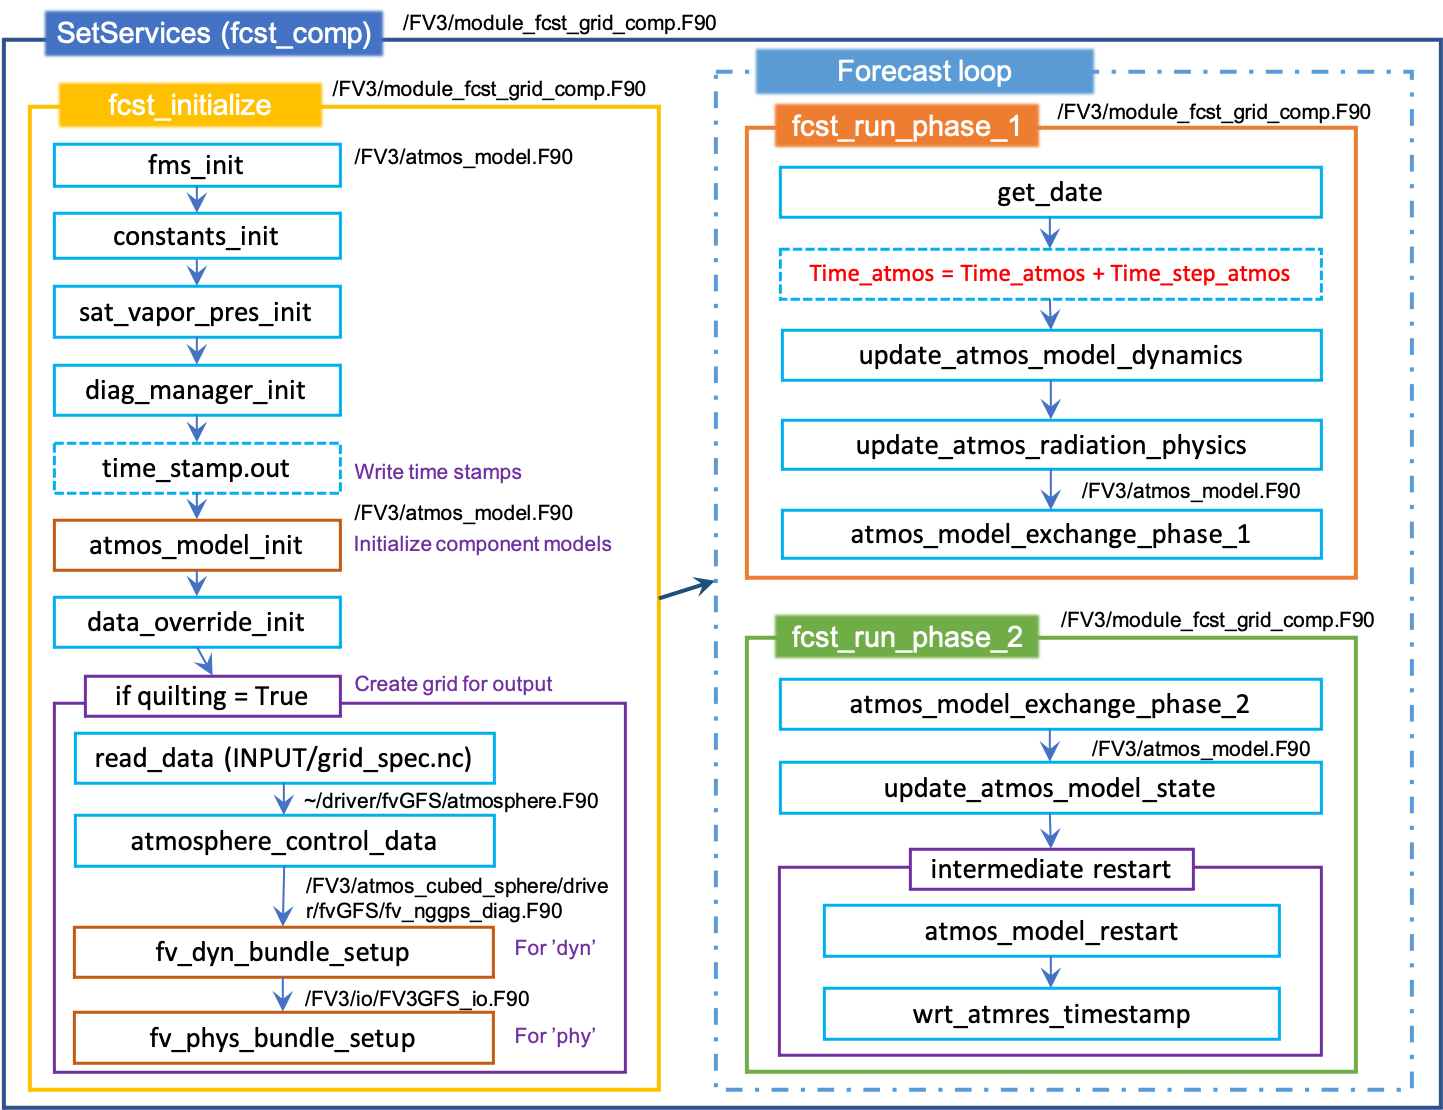
\includegraphics[width=0.73\linewidth]{fv3_struct_setservice.png}
  \caption{Structure of the UFS weather model: SetService (fcst\_comp)}
  \label{fig:fv_struct_setservice}

\vspace{0.1cm}

  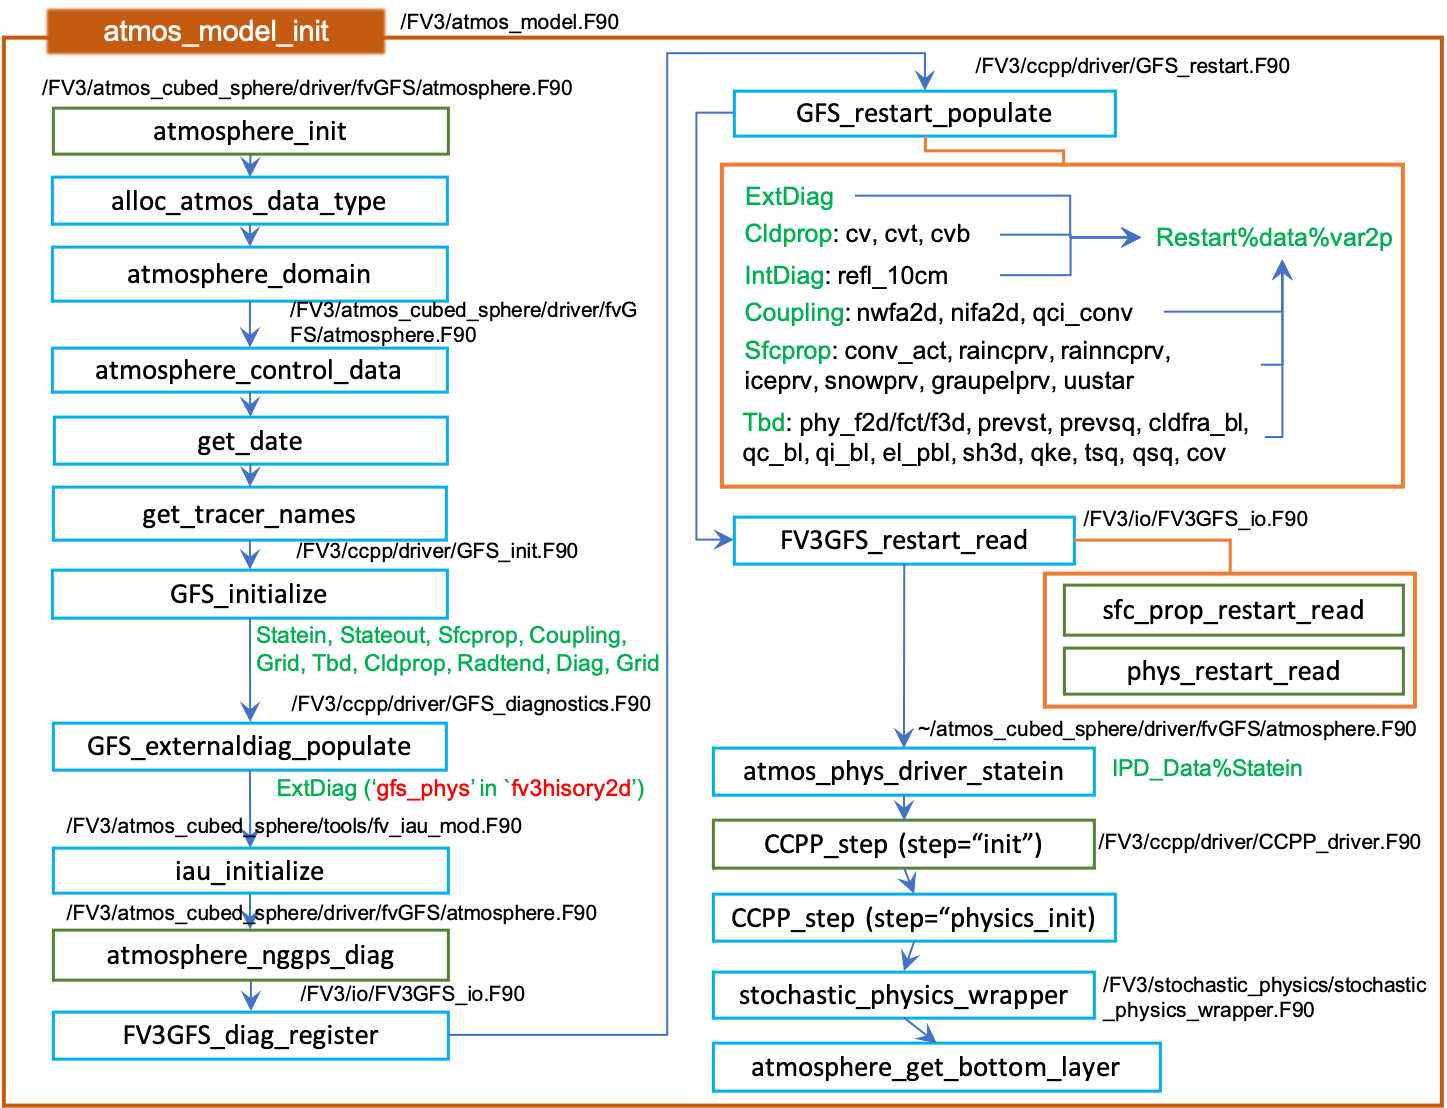
\includegraphics[width=0.73\linewidth]{fv3_struct_atmosmodelinit.png}
  \caption{Structure of the UFS weather model: atmos\_model\_init}
  \label{fig:fv_struct_atmos_model_init}
\end{figure}


\begin{figure}[ht!]
  \centering
  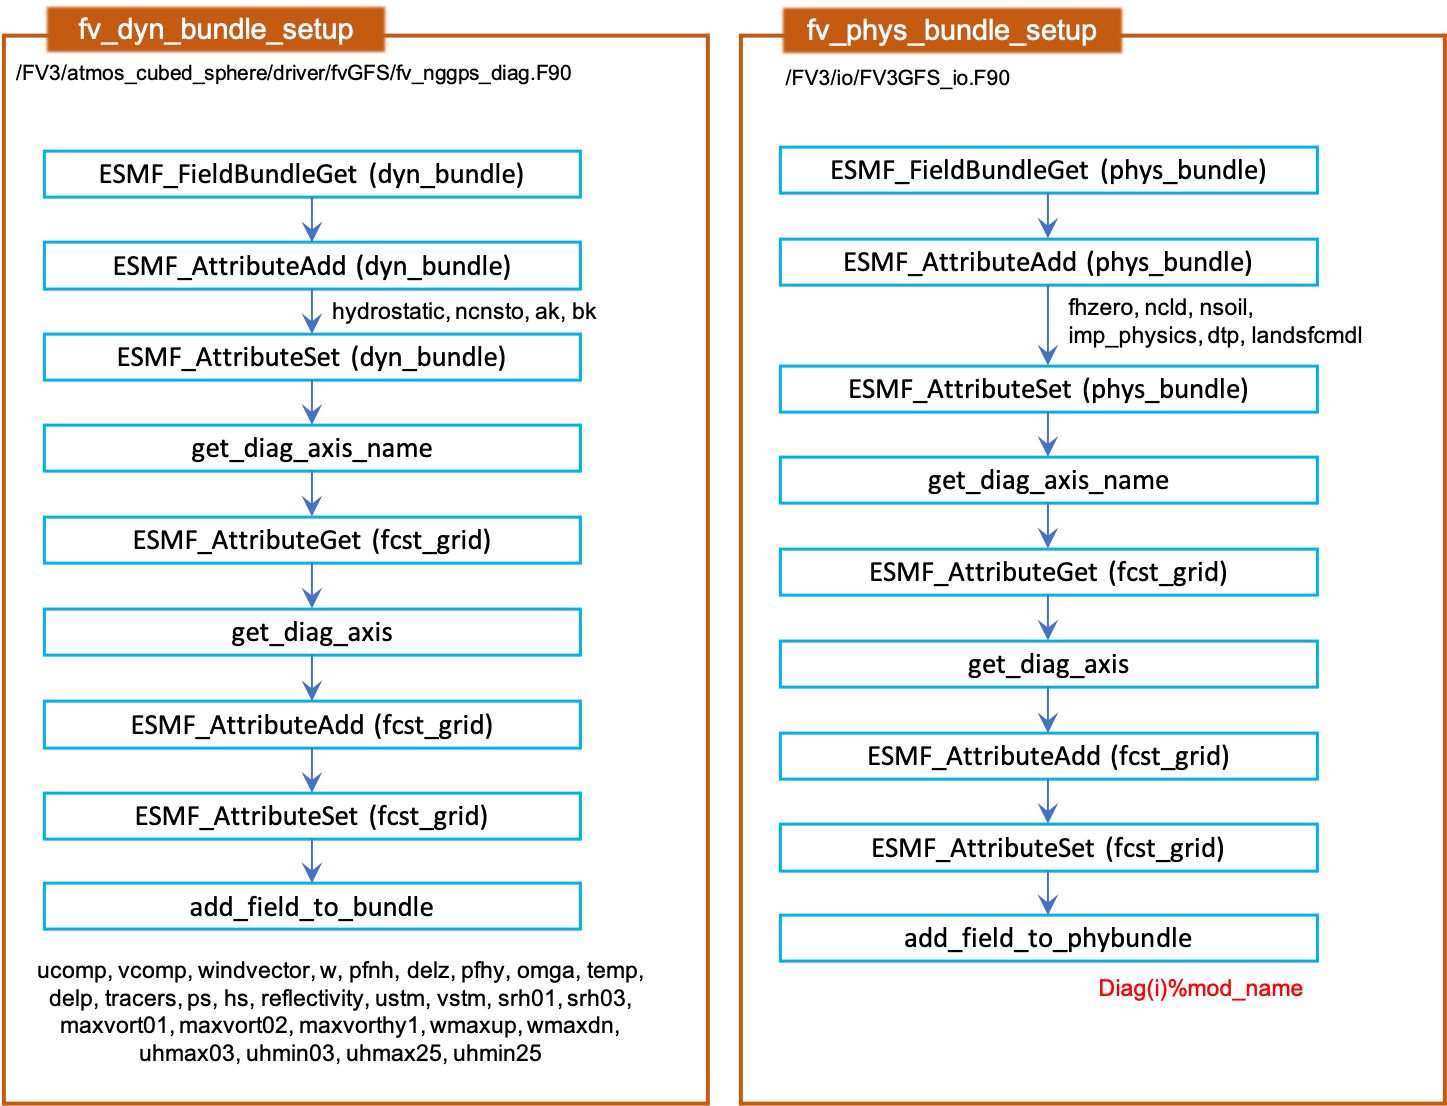
\includegraphics[width=0.73\linewidth]{fv3_struct_bundlesetup.png}
  \caption{Structure of the UFS weather model: dyn/phys\_bundle\_setup}
  \label{fig:fv_struct_bundle_setup}

\vspace{0.1cm}

  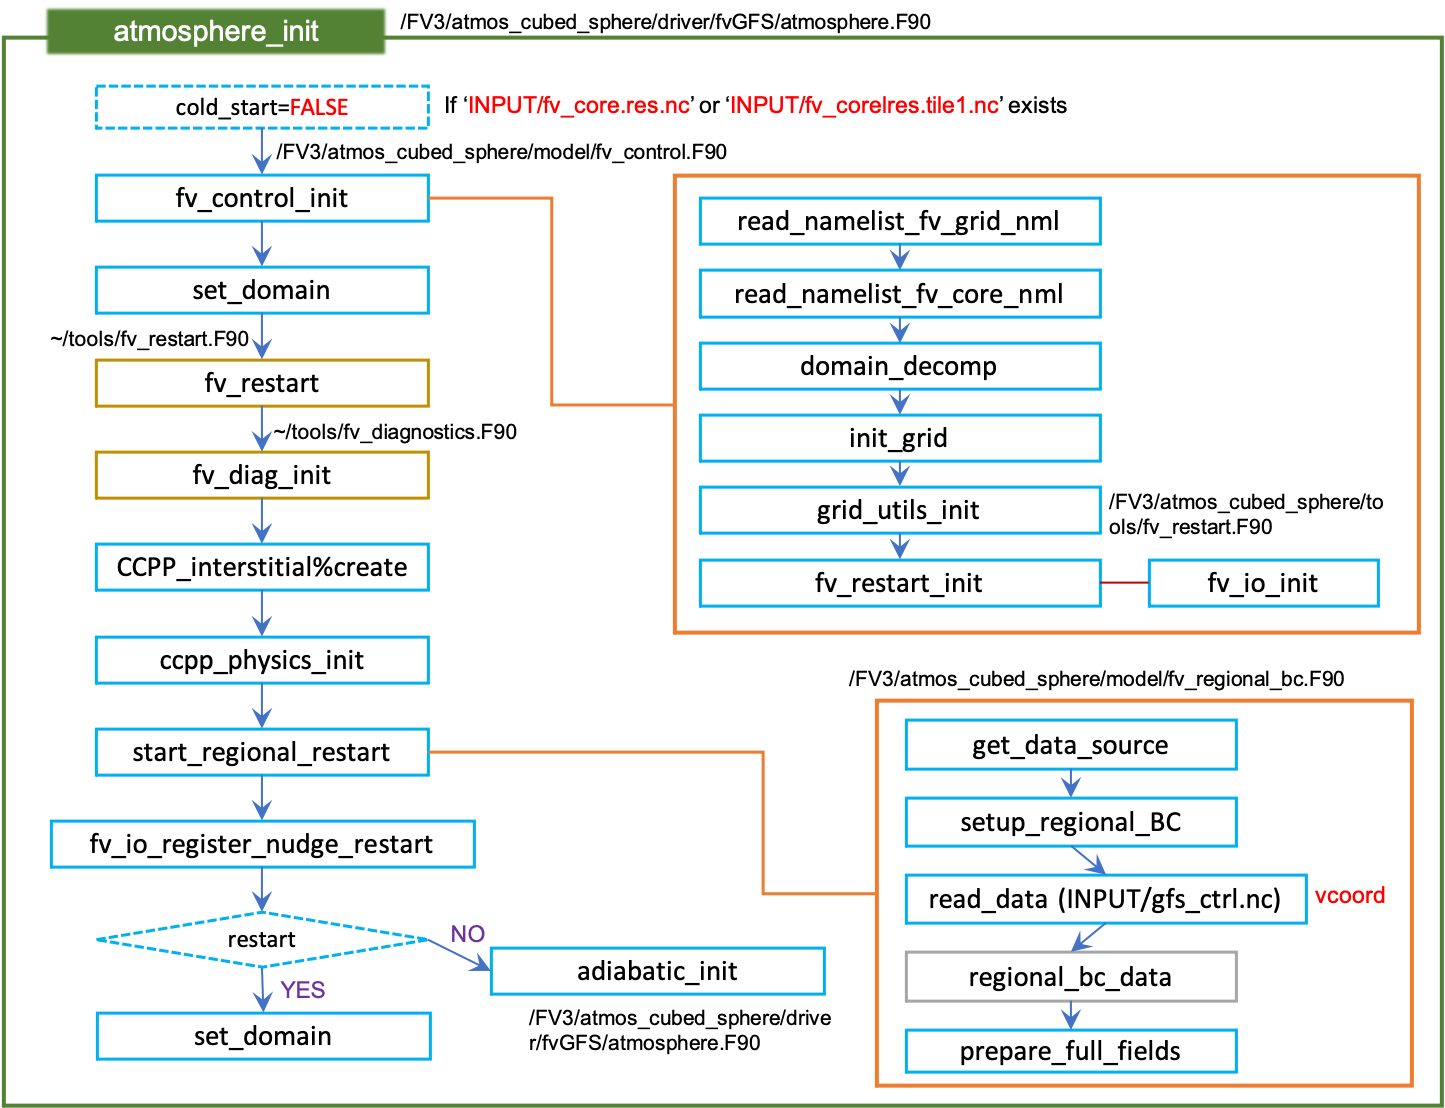
\includegraphics[width=0.73\linewidth]{fv3_struct_atmosphereinit.png}
  \caption{Structure of the UFS weather model: atmosphere\_init}
  \label{fig:fv_struct_atmosphere_init}
\end{figure}


\begin{figure}[ht!]
  \centering
  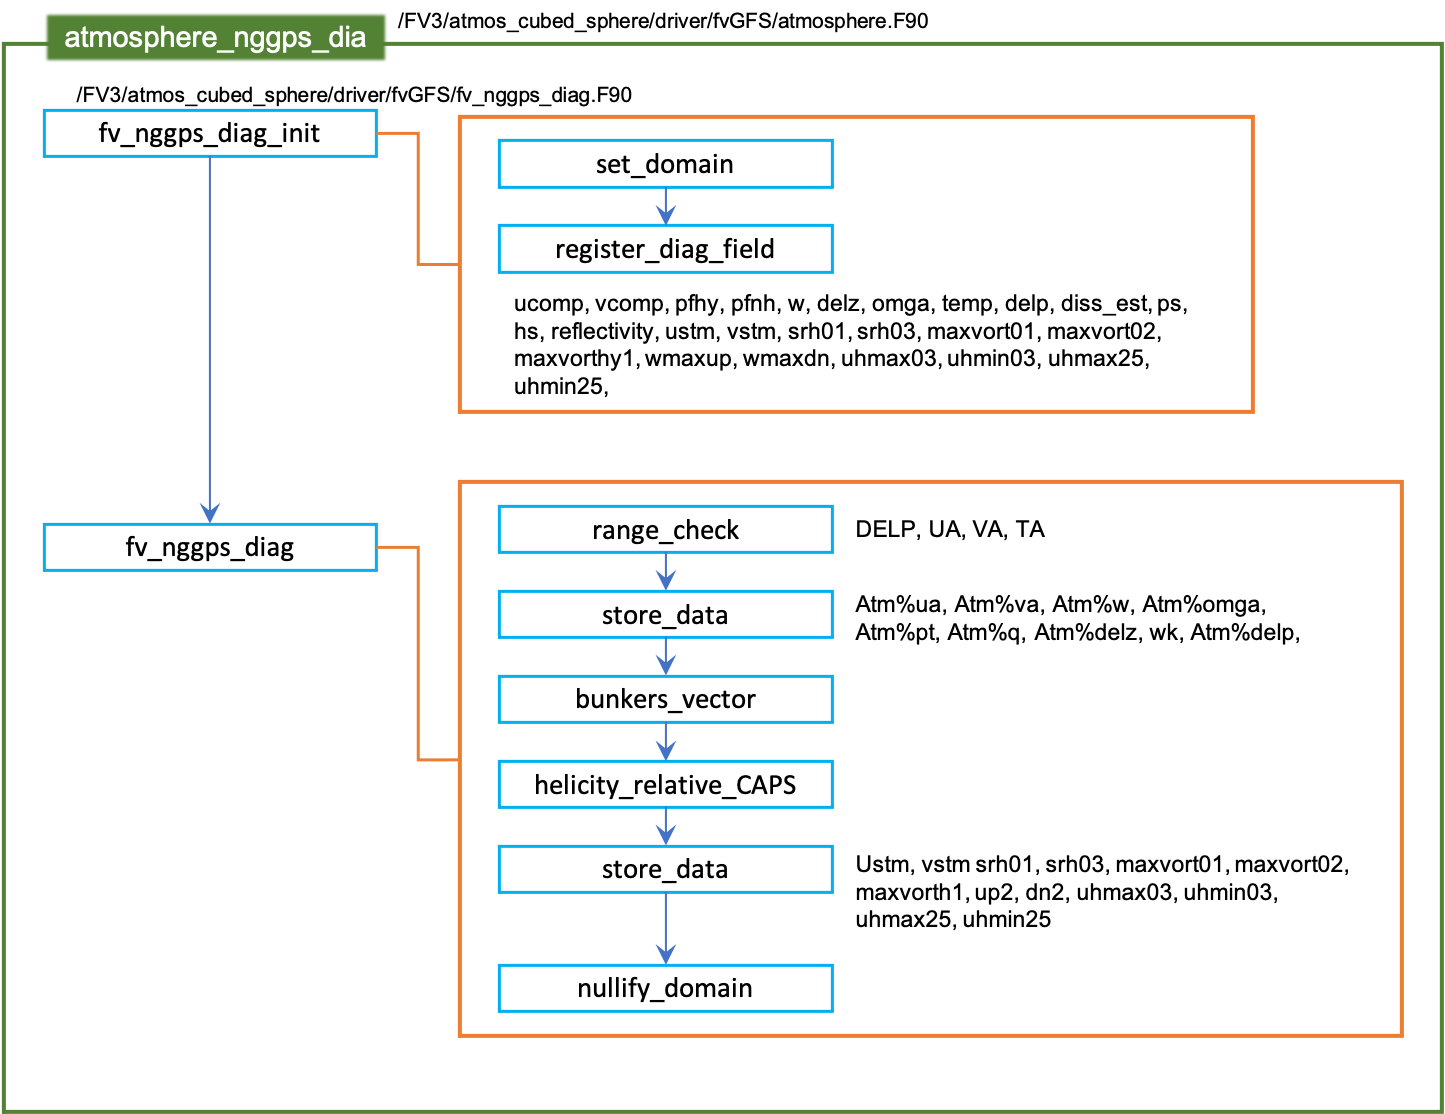
\includegraphics[width=0.73\linewidth]{fv3_struct_atmosphere_nggps_diag.png}
  \caption{Structure of the UFS weather model: atmosphere\_nggps\_diag}
  \label{fig:fv_struct_atmosphere_nggps_diag}

\vspace{0.1cm}

  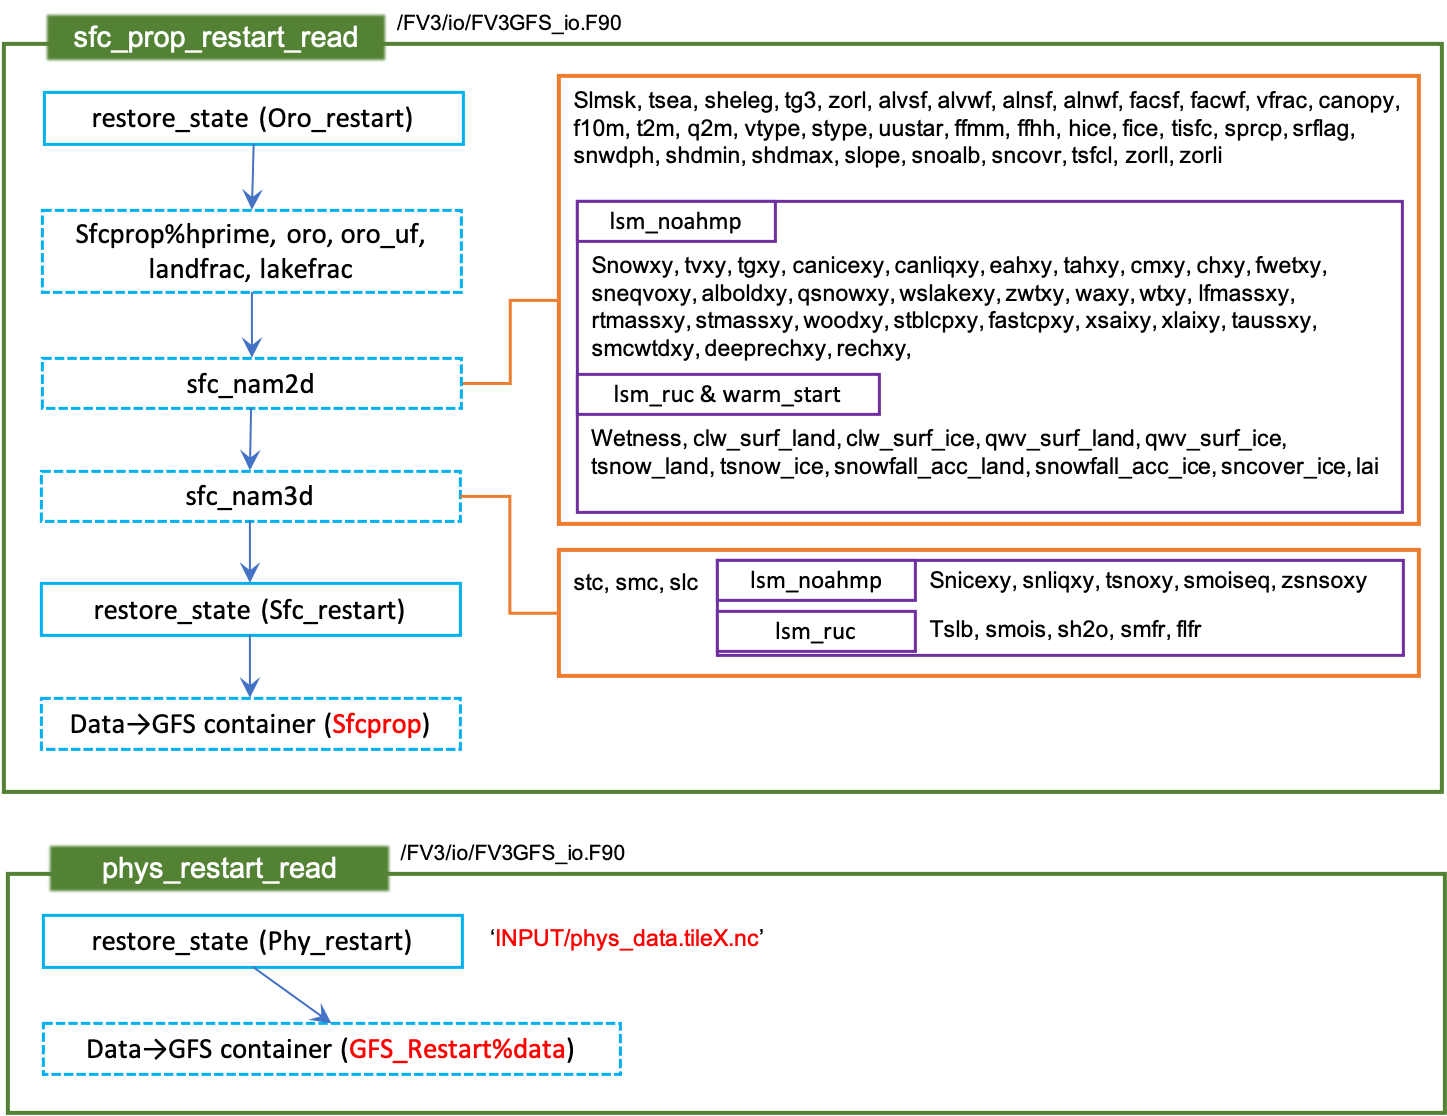
\includegraphics[width=0.73\linewidth]{fv3_struct_restart_read.png}
  \caption{Structure of the UFS weather model: restart\_read}
  \label{fig:fv_struct_restart_read}
\end{figure}


\begin{figure}[ht!]
  \centering
  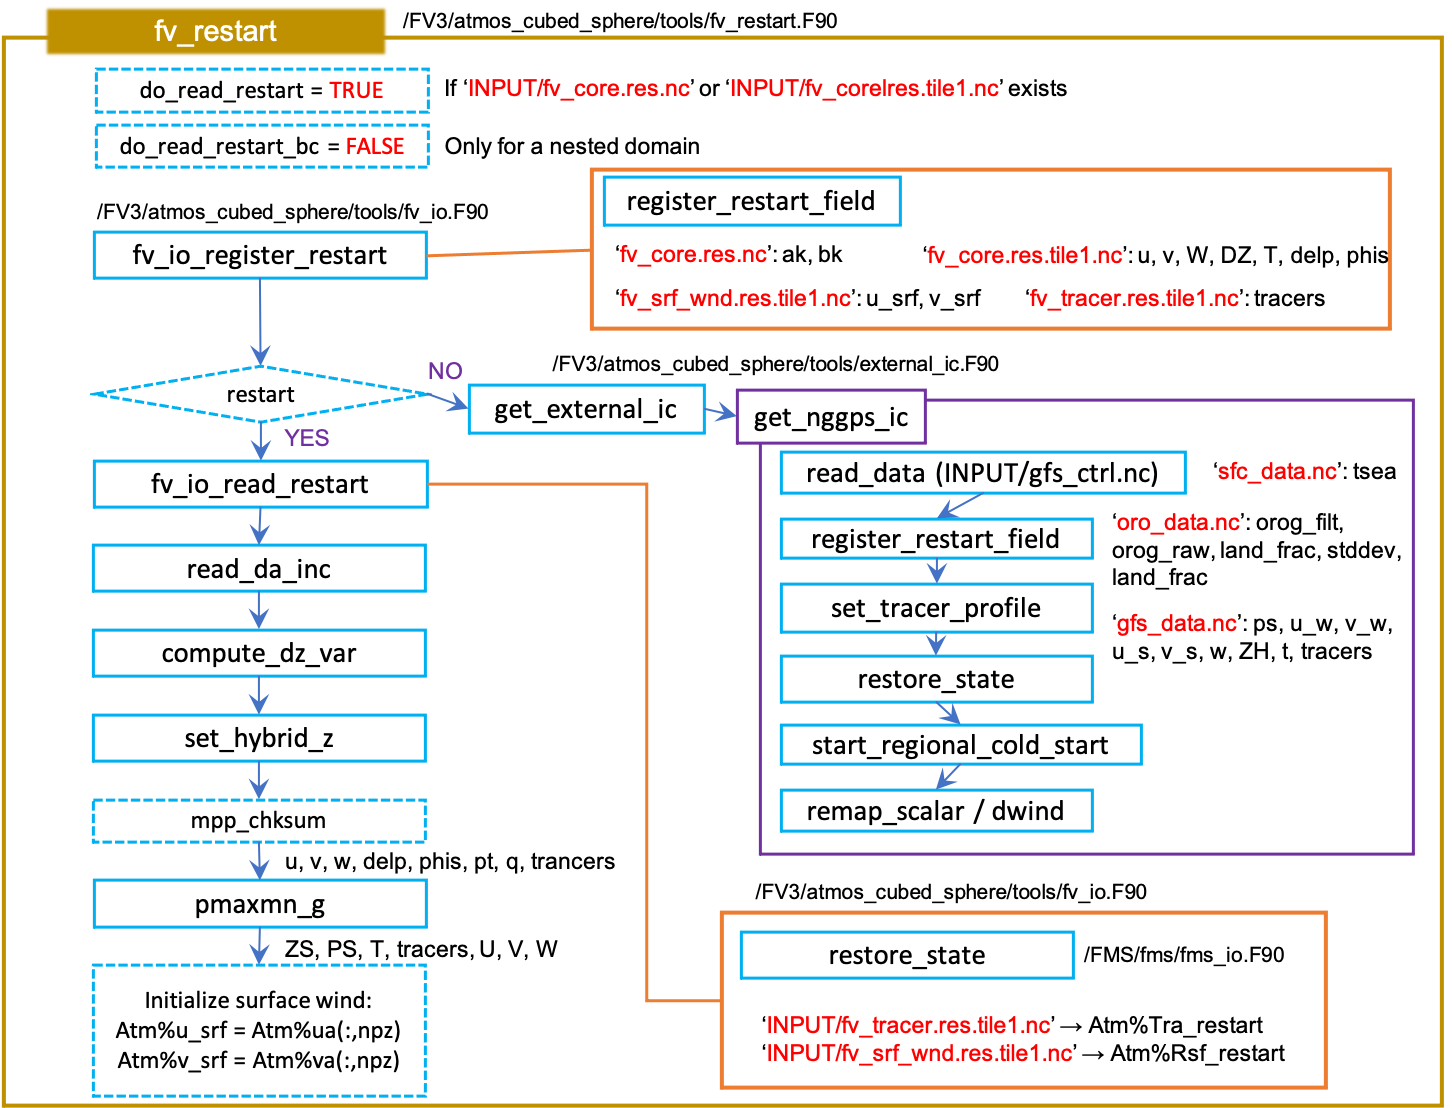
\includegraphics[width=0.73\linewidth]{fv3_struct_fvrestart.png}
  \caption{Structure of the UFS weather model: fv\_restart}
  \label{fig:fv_struct_fvrestart}

\vspace{0.1cm}

  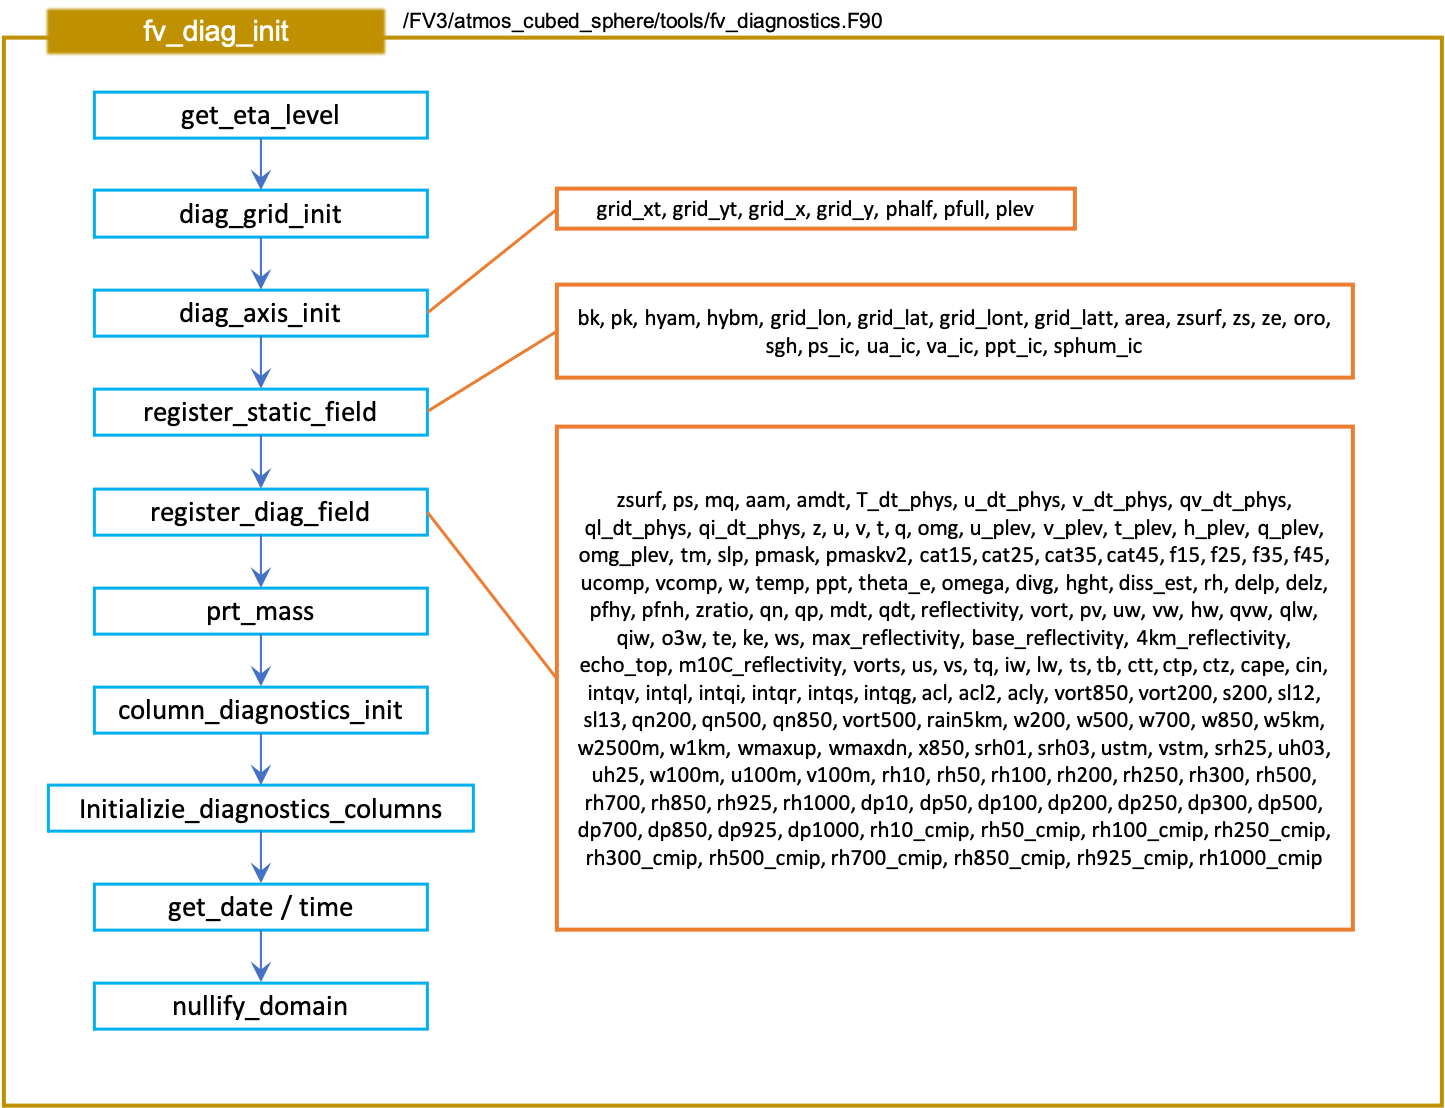
\includegraphics[width=0.73\linewidth]{fv3_struct_fvdiaginit.png}
  \caption{Structure of  the UFS weather model: fv\_diag\_init}
  \label{fig:fv_struct_fvdiaginit}
\end{figure}





%=================================================== 
\section{Compiling the UFS Weather Model}
\label{sec:build_ufs_weather_model}

%-------------------------------------------
\subsection{Building in the \{UFS\_HOME\} Directoy}

{\bf Reference)} \url{http://ufs-weather-model.readthedocs.io/} (Chapter 3.3)

\vspace{0.3cm}

Clone the `develop' branch of the UFS weather model:
\lstset{language=bash}   
\begin{lstlisting}[frame=trBL]
git clone https://github.com/ufs-community/ufs-weather-model
cd ufs-weather-model
git submodule update --init --recursive
\end{lstlisting}
The cloned directory (`$\sim$/ufs-weather-model') is referred to as `\{UFS\_HOME\}'. You can follow the steps described in Sections \ref{subsec:config_git_remote_ufs_weather} to \ref{subsec:config_git_remote_subcomp} for submitting a PR in the future.

\vspace{0.5cm}

Load the required modules and set the environment variables:
\lstset{language=bash}   
\begin{lstlisting}[frame=trBL]
cd {UFS_HOME}
vim COMPILE.sh

#!/bin/bash
set -xue
export SRC="/scratch2/NCEPDEV/fv3-cam/Chan-hoo.Jeon/ufs-weather-model"
export CCPP_SUITES="FV3_GFS_v15_thompson_mynn"
module use ${SRC}/modulefiles/hera.intel
module load fv3
cd ${SRC}
sh build.sh
\end{lstlisting}

\vspace{0.3cm}

Check the configuration:
\lstset{language=bash}   
\begin{lstlisting}[frame=trBL]
vim CMakeLists.txt (lines 21-35)
\end{lstlisting}
where the default values are
{
\fontsize{10}{12}\selectfont
\begin{longtable}{ p{0.22\linewidth} | p{0.5\linewidth} | p{0.08\linewidth} }
\hline
\hline
 Flag name & Description & Default \\
\hline
 32BIT & Single precision arithmetic in dycore & OFF \\
 AVX2 & AVX2 instruction set & ON \\
 SIMDMULTIARCH & Multi-target SIMD instruction sets & OFF \\
 DEBUG & DEBUG mode & OFF \\
 DEBUG\_LINKMPI & Linkmpi option when DEBUG mode is on & ON \\
 INLINE\_POST & Inline post & OFF \\
 MULTI\_GASES & MULTI\_GASES & OFF \\
 OPENMP & OpenMP threading & ON \\
 PARALLEL\_NETCDF & Parallel NetCDF & OFF \\
 QUAD\_PRECISION & Quad precision for certain grid metric terms in dycore & ON \\
 REPRO & REPRO mode & OFF \\
 WW3 & WW3 & OFF \\
 S2S & S2S & OFF \\
 JEDI\_DRIVER & JEDI as top level driver & OFF \\
 DATM & Data atmosphere & OFF \\
\hline
\caption{Configuration flags and their default value}
\label{table:ufs_weather_config_default}
\end{longtable}
}

Run the script:
\lstset{language=bash}   
\begin{lstlisting}[frame=trBL]
sh COMPILE.sh
\end{lstlisting}

\vspace{0.3cm}

Check if the executable `ufs\_model' is created in the `build' directory:
\lstset{language=bash}   
\begin{lstlisting}[frame=trBL]
cd {UFS_HOME}/build/
\end{lstlisting}


%-------------------------------------------
\subsection{Building in the `\{UFS\_HOME\}/tests' Directory}

\lstset{language=bash}   
\begin{lstlisting}[frame=trBL]
cd {UFS_HOME}/tests/
(rm -rf build_fv3_32bit)
sh compile.sh ${BUILD_TARGET} ${MAKE_OPT} ${BUILD_NAME} ${clean_before} ${clean_after} >& log.txt
\end{lstlisting}
where
{
\fontsize{10}{12}\selectfont
\begin{longtable}{p{0.17\linewidth} | p{0.75\linewidth} }
\hline
\hline
 Name & Description \\
\hline
 BUILD\_TARGET & Machine specific name and compiler \\
 MAKE\_OPT & Compile option for 32 bit (``32BIT=Y'') \\
 BUILD\_NAME & Sub-name of the executable (`fv3\_(?).exe') \\
 clean\_before & Flag for cleaning the entire code before compiling (YES or NO) \\
 clean\_after & Flag for cleaning the entire code after the compilation is done (YES or NO) \\
\hline
\caption{Variables for compiling.}
\label{table:fv3_var_compile}
\end{longtable}
}

\begin{itemize}
\item On Hera:
\lstset{language=bash}   
\begin{lstlisting}[frame=trBL]
cd {UFS_HOME}/tests/
sh compile.sh hera.intel "32BIT=Y STATIC=Y SUITES=FV3_GFS_v15_thompson_mynn" 32bit YES NO >& log.txt &
# check if the executable 'fv3_32bit.exe' exists.
\end{lstlisting} 

\item On WCOSS Dell (Mars/Venus):
\lstset{language=bash}   
\begin{lstlisting}[frame=trBL]
cd {UFS_HOME}/tests/
sh compile.sh wcoss_dell_p3 "32BIT=Y STATIC=Y SUITES=FV3_GFS_v15_thompson_mynn" 32bit YES NO >& log.txt &
# check if the executable 'fv3_32bit.exe' exists.
\end{lstlisting} 


\end{itemize}

{\bf Note)} For an older version, the path to the source code should be added before \{BUILD\_TARGET\} as follows:
\lstset{language=bash}   
\begin{lstlisting}[frame=trBL]
sh compile.sh {UFS_HOME} hera.intel "32BIT=Y STATIC=Y SUITES=FV3_GFS_v15_thompson_mynn" 32bit YES NO >& log.txt &
\end{lstlisting} 



%-------------------------------------------
\subsection{Building the DEBUG mode}

For the purpose of debugging, the UFS weather model can be compiled with the debug mode. You need to put the flag for debugging (``DEBUG=Y'') into the list of compile options:
\lstset{language=bash}   
\begin{lstlisting}[frame=trBL]
cd {UFS_HOME}/tests
module purge
sh compile.sh hera.intel "DEBUG=Y 32BIT=Y SUITES=FV3_GFS_v15_thompson_mynn" 32bit YES NO >& log.txt
\end{lstlisting}



%=================================================== 
\section{Regression Test}
\label{sec:dev_regression}

%-------------------------------------------
\subsection{Running Regression Test}

{\bf Reference)} \href{https://github.com/ufs-community/ufs-weather-model/wiki/Running-regression-test-using-rt.sh}{Link to UFS-weather-model regression-test wiki} 

\vspace{0.3cm}

Check the HPC account (`ACCNR') that you can use for the specific HPC machine:
\lstset{language=bash}   
\begin{lstlisting}[frame=trBL]
cd ~/ufs-weather-model/tests/
vim rt.sh
# For example, ACCNR=fv3-cam for hera (line 214)
\end{lstlisting}

Run the script with necessary flags:

\lstset{language=bash}   
\begin{lstlisting}[frame=trBL]
cd ~/ufs-weather-model/tests/
./rt.sh -e (or -r) &> log_file
\end{lstlisting}
where
{
\fontsize{10}{12}\selectfont
\begin{longtable}{p{0.1\linewidth} | p{0.4\linewidth} }
\hline
\hline
 Flag & Description \\
\hline
 -c & Create new baseline results \\
 -e & Use {\it ecFlow} workflow manager \\
 -h & Display this help \\
 -k & Keep run directory \\
 -l & Runs test specified in <file> (-l <file>) \\
 -m & Compare against new baseline results  \\
 -n & Run single test <name> (-n <name>) \\
 -r & Use {\it Rocoto} workflow manager \\
\hline
\caption{Flags for the regression test}
\label{table:flag_regression}
\end{longtable}
}

{\bf Notes)} 
\begin{itemize}
\item You do NOT need to compile the UFS weather model separately.
\item If you run a test with the flag `-k', you will find the run directories in the machine-specific path (`PTMP') specified in `ufs-weather-model/tests/ rt.sh'.
\end{itemize}


%-------------------------------------------
\subsection{Building a Specific Test Case from Regression Test}

{\bf Reference)} \href{https://ufs-weather-model.readthedocs.io/en/ufs-v1.1.0/FAQ.html#how-do-i-build-and-run-a-single-test-of-the-ufs-weather-model}{Link to UFS-weather-model FAQ} 

\vspace{0.3cm}

Specific test cases of the UFS Weather Model can be built by the regression test (`rt.sh'). The advantages of this approach are as follows:
\begin{itemize}
\item A workflow, pre- and post-processing steps are not necessary.
\item The input data required for any specific machines are already set up.
\item Working copies that be used for code-development are generated in the run directory.
\item A batch submission script (named `job\_card') is generated in the working copy.
\end{itemize}

The steps are as follows:
\begin{enumerate}
\item Create a custom configuration file from the built-in configuration file: 
\lstset{language=bash}   
\begin{lstlisting}[frame=trBL]
cd ~/ufs-weather-model/tests/
cp rt.conf my_rt.conf
vim my_rt.conf
\end{lstlisting}

\item Edit the configuration file for a specific test as needed. Two lines are essential for any custom cases: `COMPILE' and `RUN'.
\begin{enumerate}
\item COMPILE:
\lstset{language=bash,basicstyle=\scriptsize}   
\begin{lstlisting}[frame=trBL]
COMPILE | (configuration flag described in Table 9.2) | (machine & compiler) | (-) | (-)
\end{lstlisting}

\item RUN:
\lstset{language=bash,basicstyle=\scriptsize}   
\begin{lstlisting}[frame=trBL]
RUN | (parameter file in `ufs_weather_model/tests/tests) | (-) | (-) | (-)
\end{lstlisting}

\end{enumerate}

Below is an example for a regional test case with four specific run directories using the `FV3\_GFS\_15\_thompson\_mynn' CCPP suite and the flag `32BIT=Y':

\lstset{language=bash}   
\begin{lstlisting}[frame=trBL,basicstyle=\scriptsize]
COMPILE | SUITES=FV3_GFS_v15_thompson_mynn 32BIT=Y   |         | fv3 |
RUN          | fv3_ccpp_regional_control                                              |         | fv3 |
RUN          | fv3_ccpp_regional_restart                                               |         | fv3 | fv3_ccpp_regional_control
RUN          | fv3_ccpp_regional_quilt                                                  |         | fv3 |
RUN          | fv3_ccpp_regional_quilt_netcdf_parallel                        |         | fv3 |
\end{lstlisting}

\item Modify the machine-specific parameters in the `rt.sh' script:

\lstset{language=bash}   
\begin{lstlisting}[frame=trBL]
vim rt.sh

# specify the following parameters:
  ACCNR=(account name)
  dprefix=(output directory)
\end{lstlisting}

\item Run the `rt.sh' script:
\lstset{language=bash}   
\begin{lstlisting}[frame=trBL]
./rt.sh -k -l my_rt.conf >& my_rt.out &
\end{lstlisting}

\item Modify the input files as needed, and re-run the test case by submitting the `job\_card' file:
\lstset{language=bash}   
\begin{lstlisting}[frame=trBL]
cd {expt_dir}
sbatch job_card
(or bsub job_card)
\end{lstlisting}

\end{enumerate}

{\bf Note)} You can find another example for a restart run in Section \ref{subsec:rt_restart_build}.



%=================================================== 
\section{Unit Test}
\label{sec:dev_utest}

Reference) \href{https://github.com/ufs-community/ufs-weather-model/wiki/Running-unit-tests-using-utest}{Link to the UFS-weather-model unit-test wiki}

\vspace{0.3cm}

The unit test is a suite of tests and its purpose is to satisfy the operational implementation requirement. Compared to the regression test, the unit test focuses on the specific CCPP suite and inspects various reproducibility aspects such as threads, MPI processes, domain decomposition, and restart.  Developers ensure their implementations pass the unit test before requesting a Pull Request (PR). \\

{\bf Note)} The unit test for FV3-LAM was {\bf NOT} developed yet  as of 11/10/20. 

%-------------------------------------------
\subsection{Components of the Unit Test}

\begin{enumerate}
\item Thread reproducibility (THR):
\begin{itemize}
\item Variable: Number of threads
\item Number of threads=2, tasks per node=2
\end{itemize}
\item MPI process reproducibility (MPI):
\begin{itemize}
\item Variable: Number of MPI tasks
\item JNPES=2, WRITE\_GROUP=2, WRTTASK\_PER\_GROUP=12
\end{itemize}
\item Domain decomposition reproducibility (DCP):
\begin{itemize}
\item Variable: Tile layout of FV3
\item Swap `INPES' and `JNPES'
\end{itemize}
\item Restart reproducibility (RST):
\begin{itemize}
\item Use restart files in the middle of the run (SHOUR+FHMAX/2) and compare results at the end of the run (SHOUR+FHMAX).
\end{itemize}
\item 64/32 (BIT)
\item Debug (DBG)
\end{enumerate}


%-------------------------------------------
\subsection{Running Unit Test}

\begin{enumerate}
\item Pick a test case under `$\sim$/ufs-weather-model/tests/tests' that is relevant to the code change.
\item Modify the test case or add a new test case.
\item Run the test case.

\lstset{language=bash}   
\begin{lstlisting}[frame=trBL]
cd ~/ufs-weather-model/tests
./utest -n <test-name>
\end{lstlisting}
where
{
\fontsize{10}{12}\selectfont
\begin{longtable}{ p{0.1\linewidth} | p{0.5\linewidth} }
\hline
\hline
 Flag & Description \\
\hline
 -n & Run all unit tests for <test-name> (-n <test-name>) \\
 -c & Runs a specific unit test case (-c <test-case>) \\
 -h & Display usage of shell script \\
 -k & Keep the run directory \\
 -e & Use {\it ecFlow} workflow manager \\
 -x & Skip compilation \\
 -z & Skip running (compilation only) \\
 -b & Test bit reproducibility \\
 -d & Test debug reproducibility \\
\hline
\caption{Flags for the unit test}
\label{table:flag_unit_test}
\end{longtable}
}

For examples, in case of <test-name>=`fv3\_ccpp\_control':
\begin{enumerate}
\item To run all tests:
\lstset{language=bash}   
\begin{lstlisting}[frame=trBL]
./utest -n fv3_ccpp_control
\end{lstlisting}

\item To run THR test only:
\lstset{language=bash}   
\begin{lstlisting}[frame=trBL]
./utest -n fv3_ccpp_control -c thr
\end{lstlisting}

\item To run MPI and DCP tests only:
\lstset{language=bash}   
\begin{lstlisting}[frame=trBL]
./utest -n fv3_ccpp_control -c mpi,dcp
\end{lstlisting}

\end{enumerate}


\item Check and commit the unit test report/logfile to the developer's feature branch.
\end{enumerate}


%-------------------------------------------
\subsection{Input and Output}

\begin{enumerate}
\item Input
\begin{itemize}
\item `utest.bld'
\lstset{language=bash}   
\begin{lstlisting}[frame=trBL]
cd ~/ufs-weather-model/tests
vim utest.bld
\end{lstlisting}
\begin{itemize}
\item Specify the required build options in the format of `<test-name> | <build\_opt>'.
\item <build\_opt> can be `WW3=Y', `CCPP=Y', etc.
\item <test-name>, <INPUT\_NML>, <FV3\_RUN>: all similar to those in the regression test
\end{itemize}
\end{itemize}

\item Output
\begin{itemize}
\item File location: `$\sim$/ufs-weather-model/tests/'
\item Unit test logfile: `UnitTests\_[machine]\_[compiler].log' (commit)
\item Compile logfile: `Compile\_ut\_[machine]\_[compiler].log'
\item Directory: `log\_ut\_[machine].[compiler]
\end{itemize}

{\bf Note)} Do not commit the `Compile\_ut\_[machine]\_[compiler].log' and `log\_ut\_[machine]. [compiler] files.

\end{enumerate}




%=================================================== 
\section{Initial and Lateral Boundary Fields}
\label{sec:dev_sar_icbc}

%-------------------------------------------
\subsection{Source Codes}

Almost all modification for regional IC/LBC can be found at
\lstset{language=bash}   
\begin{lstlisting}[frame=trBL]
cd ~/ufs-weather-model/FV3/atmos_cubed_sphere/model/
vim fv_regional_bc.F90
\end{lstlisting}

Sometimes it happens at
\lstset{language=bash}   
\begin{lstlisting}[frame=trBL]
cd ~/ufs-weather-model/FV3/atmos_cubed_sphere/tools/
vim external_ic.F90
\end{lstlisting}



%-------------------------------------------
\subsection{Regional Boundary Update}

Figure \ref{fig:regional_bc_update_u} illustrates the halo and blending zones of the longitudinal ($u$) velocity field updated by the `regional\_boundary\_update' call. In general, the scalar variables such as `delp' and `pt', and the vertical velocity `w' have three halo rows in both $i$ and $j$ directions along the boundary. However, the velocity fields such as `u', `v', `ut', and `vt' have one more layer. The variables of `u' and `vt' have four halo rows in the $j$ direction while the variables of `v' and `ut' have four halo rows in the $i$ direction. 

\begin{figure}[ht!]
  \centering
  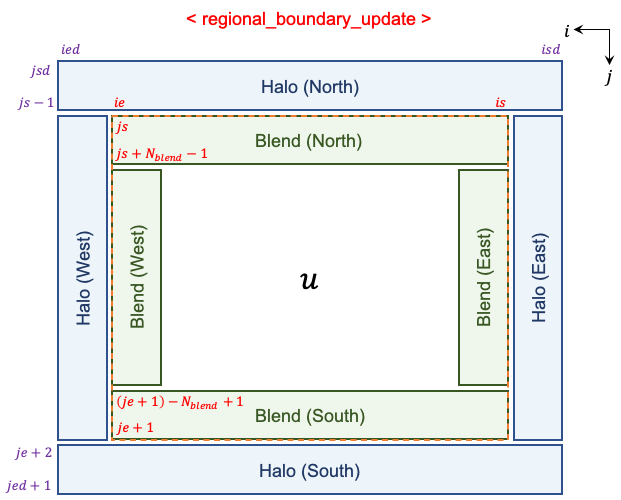
\includegraphics[width=0.5\linewidth]{regional_bc_update.png}
  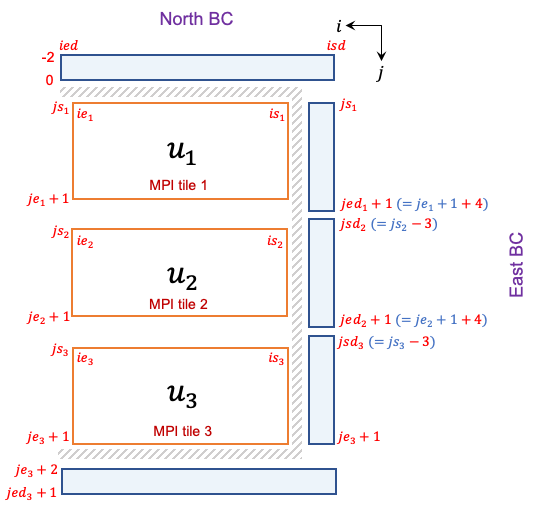
\includegraphics[width=0.43\linewidth]{regional_bc_tiles.png}
  \caption{Regional boundary update: $u$ field}
  \label{fig:regional_bc_update_u}
\end{figure}





%=================================================== 
\section{Restart Option: Warm Start}                 
\label{sec:workflow_restart}

%-------------------------------------------
\subsection{Regression Test for a Regional Restart}
\label{subsec:rt_restart_build}

Clone the latest `develop' branch of the UFS weather model:
\lstset{language=bash}   
\begin{lstlisting}[frame=trBL]
git clone https://github.com/ufs-community/ufs-weather-model
cd ufs-weather-model
git submodule update --init --recursive
\end{lstlisting}

Check the HPC account (`ACCNR') that you can use for the specific HPC machine:
\lstset{language=bash}   
\begin{lstlisting}[frame=trBL]
cd ~/ufs-weather-model/tests/
vim rt.sh
# For example, ACCNR=fv3-cam for hera (line 214)
\end{lstlisting}

Open the configuration file of the regression test:
\lstset{language=bash}   
\begin{lstlisting}[frame=trBL]
vim rt.conf
\end{lstlisting}

Edit only for two tests of control and restart as follows (remove all the rest):
\lstset{language=bash}   
\begin{lstlisting}[frame=trBL, basicstyle=\scriptsize]
COMPILE | SUITES=FV3_GFS_v15_thompson_mynn 32BIT=Y   |    | fv3 |
RUN     | fv3_ccpp_regional_control                  |    | fv3 |
RUN     | fv3_ccpp_regional_restart                  |    | fv3 | fv3_ccpp_regional_control
\end{lstlisting}

Run the regression test 
\lstset{language=bash}   
\begin{lstlisting}[frame=trBL]
./rt.sh -ek
\end{lstlisting}


The three directories should be created as below. All output NetCDF files in control (2) and restart (3) should be bitwise identical.
\lstset{language=bash}   
\begin{lstlisting}[frame=trBL]
cd /scratch1/NCEPDEV/stmp2/Chan-hoo.Jeon/FV3_RT/rt_#     (on Hera)
\end{lstlisting}

\begin{enumerate}
\item compile\_1
\item fv3\_ccpp\_regional\_control\_prod
\item fv3\_ccpp\_regional\_restart\_prod
\end{enumerate}
{\bf Note)} You can check the machine-specific path (`PTMP') in `ufs-weather-model/ tests/rt.sh'.



%-------------------------------------------
\subsection{Checklist for a Restart Run}

\begin{enumerate}
\item The parameters listed in Table \ref{table:param_modify_restart} should be modified in `input.nml':
{
\fontsize{10}{12}\selectfont
\begin{longtable}{p{0.15\linewidth} | p{0.12\linewidth} | p{0.2\linewidth} }
\hline
\hline
 Parameter & Cold start & Warm start (restart) \\
\hline
 external\_ic & .true. & .false \\
 mountain & .false. & .true. \\
 na\_init & 1 & 0 \\
 nggps\_ic & .true. & .false. \\
 warm\_start & .false. & .true. \\ 
\hline
\caption{Parameters to be modified for a restart run}
\label{table:param_modify_restart}
\end{longtable}
}

\item Copy the input files for restart, which are presented in the `RESTART' directory, into the `INPUT' directory. 
\lstset{language=bash}   
\begin{lstlisting}[frame=trBL]
cp {base_dir}/RESTART/* {EXPTDIR}/INPUT/
\end{lstlisting}

The list of the additional input files is as follows:
{
\fontsize{10}{12}\selectfont
\begin{longtable}{p{0.25\linewidth} | p{0.55\linewidth} }
\hline
\hline
 File name & Description / variables \\
\hline
 coupler.res & Model start time and current model time \\
 fv\_core.res.nc & ak, bk \\
 fv\_core.res.tile1.nc & u, v, W, DZ, T, delp, phis\\
 fv\_srf\_wnd.res.tile1.nc & u\_srf, v\_srf \\
 fv\_tracer.res.tile1.nc & sphum, liq\_wat, rainwat, ice\_wat, snowwat, graupel, o3mr, sgs\_tke, cld\_amt \\
 phy\_data.nc & cv, cvt, cvb, phy\_f2d\_01, totprcp\_ave, cnvprcp\_ave, phy\_f3d\_01, phy\_f3d\_02 \\
 sfc\_data.nc & Surface climatology data \\
\hline
\caption{Additional input files for a restart run}
\label{table:add_input_restart}
\end{longtable}
}

{\bf Note)} Variables in the initial condition file `gfs\_data.nc' which is the input file of the base case: ps, w, zh, t, delp, sphum, liq\_wat, o3mr, ice\_wat, rainwat, snowwat, graupel, u\_w, v\_w, u\_s, v\_s

\end{enumerate}





%=================================================== 
\section{Near-boundary Blending}
\label{sec:dev_sar_blend}

The blending works by not only generating data for the boundary region but by inserting additional `boundary rows' into the BC files that overlap the outermost rows of the integration domain. The {\it chgres} code in `UFS\_UTILS' can add those extra rows in the boundary files. When running the forecast set the `input.nml' variable `nrows\_blend' to the number of rows you want to blend within the outer rows of the integration domain.

%-------------------------------------------
\subsection{Blending in a Forecast Run}

\begin{enumerate}

\item Check that {\it FV3}, which is installed in your system, supports the `blending' option:
\lstset{language=bash}   
\begin{lstlisting}[frame=trBL]
cd ~/ufs-weather-model/FV3/atmos_cubed_sphere/model/
grep -n -i blend fv_control.F90 fv_arrays.F90
\end{lstlisting}

\item Create IC/LBC fields including blending layers (Section \ref{chpt:sar_pre_glb2reg}).
\begin{itemize}
\item Run `chgres\_cube' with `halo\_blend':
\lstset{language=bash}   
\begin{lstlisting}[frame=trBL]
    regional = 1 (or 2)
    halo_bndy =4
    halo_blend = 10
\end{lstlisting}
\end{itemize}

\item Turn on the blending option in the configuration `input.nml' (Section \ref{subsec:input_domain_nml}).

\lstset{language=bash}   
\begin{lstlisting}[frame=trBL]
(under `&fv_core_nml')
    regional_bcs_from_gsi = .false.   (for DA blending)
    write_restart_with_bcs = .false.   (for DA blending)
    nrows_blend = 10
\end{lstlisting}
{\bf Note)} Make sure that `halo\_blend' is equal to `nrows\_blend'.

\end{enumerate}


%-------------------------------------------
\subsection{Blending in a DA Run}

\begin{enumerate}
\item Two variables in `input.nml' need to be used: (1) write\_restart\_with\_bcs (.true. / .false.), and (2) regional\_bcs\_from\_gsi (.true. / .false.). 

\begin{itemize}
\item `write\_restart\_with\_bcs':

Typically the model writes out restart files that contain only the integration domain in which case set this flag `false'. However, in order to include the boundaries in the assimilation, those boundary rows should be included in the restart files so set the first flag to `true'. This will make restart files write the boundary rows in addition to writing out normal core and tracers.

\item `regional\_bcs\_from\_gsi':

The second flag says to treat all the BC files in the usual way when it is `false'. The `usual' means that the variables are remapped in the vertical from the external forecast's layer distribution to the forecast's, and the winds are rotated from geographic lat/lon to the forecast grids' orientation. When the assimilation writes out restart files, though the fields put into the new post-GSI, BC files are already on the proper levels and are oriented properly so the model is told to {\bf NOT} remap or rotate by setting this flag to `true'.

\end{itemize}

\item To create and write the new larger restart files, which include the blending boundary layers, for the GSI, the code needs original restart files to get all the specifications and field names in the `/INPUT' subdirectory for NetCDF:

\begin{enumerate}
\item Copy any normal-sized `fv\_core.res.tile1.nc' and `fv\_tracer.res.tile1.nc' into the `/INPUT' subdirectory before starting the forecast, basically as templates. Make sure that all three dimensions in those template restart files are the values you want to use.

\item Change their names from `tile1' to `temp'. Otherwise, FMS will get confused. 

\item The forecast's normal and enlarged restart files will show up in the `/RESTART' subdirectory of the working directory as usual. The enlarged restart file names will end with `.tile1\_new.nc'.
\end{enumerate}

\item After your run writes out the two enlarged restart files for the data assimilation, you also need `sfc\_data.nc' and `grid\_spec.nc' files that have been similarly enlarged. To get them, run the following serial code:
\lstset{language=bash}   
\begin{lstlisting}[frame=trBL]
prep_for_regional_DA.F90
\end{lstlisting}

\begin{itemize}
\item Input files:
{
\fontsize{10}{12}\selectfont
\begin{longtable}{p{0.2\linewidth} | p{0.2\linewidth} | p{0.45\linewidth}   }
\hline
\hline
 Original name & Transferred name & Description  \\
\hline
 sfc\_data.tile7.nc & sfc\_data\_orig.nc & Output of IC \\
 grid\_spec.nc & grid\_spec\_orig.nc & Output of a forecast run \\
 grid.tile7.halo3.nc & grid.tile7.halo3.nc & Output of `grid\_driver' (pre-processing)\\
\hline
\caption{Input files for enlarged restart files}
\label{table:fv3_dablend_en_restart_in}
\end{longtable}
}

\item Output files:
{
\fontsize{10}{12}\selectfont
\begin{longtable}{ p{0.2\linewidth} | p{0.2\linewidth}   }
\hline
\hline
 Original name & Transferred name \\
\hline
 sfc\_data\_new.nc & sfc\_data.nc \\
 grid\_spec\_new.nc & grid\_spec.nc  \\
\hline
\caption{Output files for enlarged restart files}
\label{table:fv3_dablend_en_restart_out}
\end{longtable}
}

\end{itemize}

{\bf Note)} This job assumes that the original smaller files have been renamed `sfc\_data\_orig.nc' and `grid\_spec\_orig.nc' and it then generates the larger files called `sfc\_data\_new.nc' and `grid\_spec\_new.nc'.

\item The data assimilation runs on the enlarged core and tracers restart files and the enlarged `sfc\_data.nc' and `grid\_spec.nc' files. When it is finished, the updated data must be put back into the files the model will read in the forecast. 
\lstset{language=bash}   
\begin{lstlisting}[frame=trBL]
move_DA_update_data.F90
\end{lstlisting}

\begin{itemize}
\item Input files:
{
\fontsize{10}{12}\selectfont
\begin{longtable}{p{0.3\linewidth} | p{0.6\linewidth}   }
\hline
\hline
File name  & Description  \\
\hline
 fv\_core.res.tile1\_new.nc & Enlarged core restart file \\
 fv\_tracer.res.tile1\_new.nc & Enlarged tracers restart file \\
 gfs\_bndy.tile7.HHH.nc & Original BC file valid at the time (HHH) of the restart (no DA changes) \\
\hline
\caption{Input files for updated BC files}
\label{table:fv3_dablend_update_in}
\end{longtable}
}

\item Run:

Currently the move program takes `HHH' as a command line argument. i.e. if the BC file is `gfs\_bndy.tile7.000.nc' then to execute the program:
\lstset{language=bash}   
\begin{lstlisting}[frame=trBL]
./a.out 000
\end{lstlisting}

When the code executes it will copy all the interior data from the updated enlarged restart files back into the original-sized restart files that were written prior to running the data assimilation (both normal and enlarged restart files are written when `write\_restart\_with\_bcs = .true.'). And a new BC file is generated called `gfs\_bndy.tile7. HHH\_gsi.nc' that is taken from the boundary region of the updated enlarged restart files and it has a different structure from the original BC files.


\item Output files:
{
\fontsize{10}{12}\selectfont
\begin{longtable}{ p{0.3\linewidth} | p{0.45\linewidth}   }
\hline
\hline
 File name  & Description  \\
\hline
 gfs\_bndy.tile7.HHH\_gsi.nc &  \\
\hline
\caption{Output files for updated BC files}
\label{table:fv3_dablend_update_out}
\end{longtable}
}

\end{itemize}

\item When you start up the next free forecast following the DA update set:
\lstset{language=bash}   
\begin{lstlisting}[frame=trBL]
regional_bcs_from_gsi = .true.
\end{lstlisting}
So the model will use `gfs\_bndy.tile7.HHH\_gsi.nc' as the starting BC file (with no vertical remap or wind rotation) but then will read the following BC file valid at the end of your boundary update interval with its original name (no `\_gsi' in it) and will do the remap and wind rotation as usual.

\end{enumerate}



%-------------------------------------------
\subsection{Modification of the source code}

The code can be cloned from GitHUB:
\lstset{language=bash}   
\begin{lstlisting}[frame=trBL]
git clone https://github.com/TomBlack-NOAA/GFDL_atmos_cubed_sphere.git -b tracers
\end{lstlisting}

The files under `atmos\_cubed\_sphere' that are changed for the blending and for including the regional boundary in the data assimilation are shown in Table \ref{table:blend_dir}. Here are two versions of two files needed to switch between the NAM's 60-layer vertical structure and the 65 layers.

\begin{enumerate}
\item For 65 layers:
\lstset{language=bash}   
\begin{lstlisting}[frame=trBL]
cp external_ic.F90_65lyrs external_ic.F90
cp fv_eta.F90_65lyrs fv_eta.F90
\end{lstlisting}

\item For NAM's 60 layers:
\lstset{language=bash}   
\begin{lstlisting}[frame=trBL]
cp external_ic.F90_NAM_lyrs external_ic.F90
cp fv_eta.F90_NAM_lyrs fv_eta.F90
\end{lstlisting}

\end{enumerate}


\begin{figure}[H]
\centering
\begin{minipage}{0.5\linewidth}
\dirtree{%
.1 ufs-weather-model.
.2 FV3.
.3 atmos\_cubed\_sphere.
.4 model.
.5 fv\_arrays.F90.
.5 fv\_control.F90.
.5 fv\_regional.F90.
.4 tools.
.5 external\_ic.F90.
.5 (external\_ic.F90\_NAM\_lyrs).
.5 (external\_ic.F90\_65lyrs).
.5 fv\_eta.F90.
.5 (fv\_eta.F90\_NAM\_lyrs).
.5 (fv\_eta.F90\_65lyrs).
.5 fv\_restart.F90.
.4 driver.
.5 fvGFS.
.6 atmosphere.F90.
}
\end{minipage}
\caption{Structure of directory}
\label{table:blend_dir}
\end{figure}





%******************************************************************************************************************************************
\chapter{Code Management on GitHub}                 
\label{chpt:code_manage_github}


%=================================================== 
\section{Modification of the UFS Weather Model on GitHub}
\label{sec:mod_ufs_github}

%-------------------------------------------
\subsection{Overall Steps of Modification and Pull Request}
\label{subsec:mod_ufs_overall}

UFS applications have hierarchical structure managed through git submodules. If you are making changes in UFS sub-components, you should follow these steps:

\begin{enumerate}
\item Check the hierarchical structure of the UFS weather model.
\item Create your own forks from the repositories that you are going to make changes to.
\item Configure Git remotes for a sub-component.
\item Update the branch in the local and fork repositories.
\item Create a `feature/fix\_[xxx]' branch in the cloned sub-component.
\item Make changes to the feature branch.
\item Commit (save) the changes to the local feature branch.
\item Push the local feature branch to your remote `origin' branch (sub-component).
\item Configure Git remotes for the UFS weather model.
\item Create a feature branch in the cloned `ufs-weather-model' repository.
\item Make and commit changes if necessary.
\item Update the sub-component in the `.gitmodules' file and sync the submodules.
\item Push the local feature branch (ufs-weather-model)
\item Create pull requests (PR).
\item Update and modify the branch based on reviewers' comments.
\item Clean up the branch once your pull request is merged.
\end{enumerate}

\begin{figure}[ht!]
  \centering
  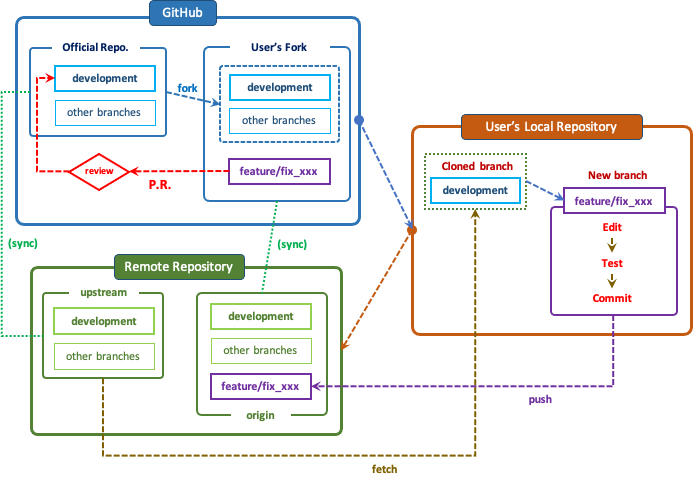
\includegraphics[width=0.8\linewidth]{github_flow.png}
  \caption{Flowchart for Pull Request (PR)}
  \label{fig:github_flow}
\end{figure}


%-------------------------------------------
\subsection{Structure of the UFS Weather Model and Its Sub-components}

{
\fontsize{10}{12}\selectfont
\begin{longtable}{ p{0.22\linewidth} | p{0.4\linewidth} | p{0.1\linewidth} }
\hline
\hline
Sub-component & Repository & Branch \\
\hline
 ufs-weather-model & ufs-community/ufs-weather-model & develop \\
 CMakeModules & NOAA-EMC/CMakeModules & develop \\
 DATM & NOAA-EMC/NEMSdatm & develop \\
 FMS & NOAA-GFDL/FMS & master \\
 FV3 & NOAA-EMC/fv3atm & develop \\
 atmos\_cubed\_sphere & NOAA-EMC/GFDL\_atmos\_cubed\_sphere & dev/emc \\
 CCPP framework & NCAR/ccpp-framework & master \\
 CCPP physics & NCAR/ccpp-physics & master \\
 NEMS & NOAA-EMC/NEMS & develop \\
 WW3 & NOAA-EMC/WW3 & develop \\
 stochastic\_physics & noaa-psd/stochastic\_physics & master \\
\hline
\caption{UFS weather model: GitHub repository and branch}
\label{table:ufs_weather_github_repo}
\end{longtable}
}

\begin{figure}[ht!]
\centering
\begin{minipage}{0.5\linewidth}
\dirtree{%
.1 ufs-weather-model.
.2 CMakeModules.
.2 DATM.
.2 FMS.
.2 FV3.
.3 atmos\_cubed\_sphere.
.3 ccpp.
.4 framework.
.4 physics.
.2 NEMS.
.2 WW3.
.2 stochastic\_physics.
}
\end{minipage}
\caption{UFS weather model and its sub-components}
\label{figure:ufs_weather_model_dir}
\end{figure}


%-------------------------------------------
\subsection{Forking the UFS Weather Model and Sub-components}

If you create forks in sub-component, make sure that you should create forks for all the repositories in the path from the sub-component up to the UFS weather model. For example, if you need to make changes in `FV3', you should create forks from the EMC's `fv3atm' repository (FV3) as well as the ufs-community's `ufs-weather-model' repository. \\

In a web browser, go to the GitHub page shown in Table \ref{table:ufs_weather_github_repo}.
\lstset{language=bash}   
\begin{lstlisting}[frame=trBL]
https://github.com/ufs-community/ufs-weather-model
https://github.com/NOAA-EMC/fv3atm
\end{lstlisting}

Press the `Fork' button on the top right. You can see the repositories in your GitHub account. The URL of your fork will be
\lstset{language=bash}   
\begin{lstlisting}[frame=trBL]
https://github.com/{GitHubID}/ufs-weather-model
https://github.com/{GitHubID}/fv3atm
\end{lstlisting}



%-------------------------------------------
\subsection{Cloning the UFS Weather Model}

Clone the UFS weather model to the `\{HOMEdir\}' directory (local repository) and check out the `develop' branch:
\lstset{language=bash}   
\begin{lstlisting}[frame=trBL]
cd {HOMEdir}
git clone https://github.com/ufs-community/ufs-weather-model 
cd ufs-weather-model
git submodule update --init --recursive
\end{lstlisting}
where `\{HOMEdir\}' is the parent directory where the `develop' branch will be cloned. 

\vspace{0.2cm}

{\bf Note)} You do not need to clone the sub-components separately.


%-------------------------------------------
\subsection{Configuring Git Remotes for the Cloned Sub-component}
\label{subsec:config_git_remote_subcomp}

Move to the bottom level of the sub-components for your changes (For example, FV3):
\lstset{language=bash}   
\begin{lstlisting}[frame=trBL]
cd {HOMEdir}/ufs-weather-model/FV3
\end{lstlisting}

When you clone your fork, git will create a remote (i.e. a pointer to a repository location) named `origin' that points to the authoritative repository. To check the list of remotes that are defined in your clone, issue the command:
\lstset{language=bash}   
\begin{lstlisting}[frame=trBL]
git remote -v
\end{lstlisting}

\begin{itemize}
\item Even though you cloned the UFS weather model, its sub-component `FV3' is linked to `NOAA-EMC/fv3atm'. Therefore, the output should be as follows:
\lstset{language=bash}   
\begin{lstlisting}[frame=trBL]
origin https://github.com/NOAA-EMC/fv3atm (fetch)
origin https://github.com/NOAA-EMC/fv3atm (push)
\end{lstlisting}
\end{itemize}

Rename the `origin' remote repository to the `upstream' remote repository:
\lstset{language=bash}   
\begin{lstlisting}[frame=trBL]
git remote rename origin upstream
\end{lstlisting}

Create a new `origin' remote repository that points to your fork `{GitHubID}/fv3atm' repository:
\lstset{language=bash}   
\begin{lstlisting}[frame=trBL]
git remote add origin https://github.com/{GitHubID}/fv3atm
git remote update
git remote -v
\end{lstlisting}

\begin{itemize}
\item The output should be as follows:
\lstset{language=bash}   
\begin{lstlisting}[frame=trBL]
origin   https://github.com/{GitHubID}/fv3atm (fetch)
origin   https://github.com/{GitHubID}/fv3atm (push)
upstream   https://github.com/NOAA-EMC/fv3atm (fetch)
upstream   https://github.com/NOAA-EMC/fv3atm (push)
\end{lstlisting}
\end{itemize}



%-------------------------------------------
\subsection{Updating the Branch in the Cloned Sub-component}

You should update the `develop' branch in your clone (local repository) as well as in your fork in order to have the latest changes in the `develop' branch of the authoritative `NOAA-EMC/fv3atm' repository.

\begin{itemize}
\item When you create new feature branches to address new issues, you start off with the latest version of `develop' in the authoritative repository in those branches.
\item Updating the `develop' branch in your clone entails merging the latest version of the `develop' branch of the `NOAA-EMC/fv3atm' into the `develop' branch of your fork.
\end{itemize}

Fetch the contents of the `upstream' repository (i.e. the `NOAA-EMC/fv3atm' repository) to your local disk:

\lstset{language=bash}   
\begin{lstlisting}[frame=trBL]
cd {HOMEdir}/ufs-weather-model/FV3
git remote -v (You should see upstream remote on the list)
\end{lstlisting}

This will fetch all the branches from the `NOAA-EMC/fv3atm' repository and put them on your local disk. However it will not automatically check any of them out.
\begin{itemize}
\item You can see which branch you are currently on (branch with an asterisk):
\lstset{language=bash}   
\begin{lstlisting}[frame=trBL]
git branch -vva
\end{lstlisting}
There should be a list of remote branches which include the one you want to merge into your local `develop' branch.
\end{itemize}

Merge the `remote/upstream/develop' branch into your local `develop' branch:
\lstset{language=bash}   
\begin{lstlisting}[frame=trBL]
git checkout develop
git pull upstream develop (or `git fetch upstream' then `git merge upstream/develop')
\end{lstlisting}
Your local `develop' branch will now be an exact copy of the latest version of the `develop' branch of the `NOAA-EMC/regional\_workflow' repository.

\begin{itemize}
\item It is recommended not to make your own changes to your local `develop' branch.
\item Any changes you make to address issues should be made in a separate feature branch.
\item Keeping your local `develop' branch unchanged (except for occasionally updating it with the latest from the authoritative branch) allows you
\begin{enumerate}
\item to merge the latest changes from other developers into your feature branch.
\item to quickly create a new and up-to-date feature branch whenever you need to address a new issue.
\end{enumerate}
\end{itemize}

Update the `develop' branch in your fork. You can do this by pushing your updated local `develop' branch to your fork.
\lstset{language=bash}   
\begin{lstlisting}[frame=trBL]
git push origin develop
(GitHub Username)
(GitHub Password)
\end{lstlisting}



%-------------------------------------------
\subsection{Creating a New Feature Branch of the Sub-component}

\begin{itemize}
\item It is suggested that users create their own feature branch in their fork.
\item Code changes will be committed (pushed) to users' feature branch in their own fork testing.
\item Users' develop/feature branch in their fork should be synced with authoritative (official) repository periodically.
\item When development work is done, users will sync their feature branch with the latest develop (or master) branch in the authoritative repository, run the regression test and make a pull request (PR) to the authoritative repository.
\item It is suggested to delete the feature branch in users' personal fork when the code changes are merged into the authoritative repository.
\end{itemize}

Make sure that you are on the local `develop' branch:
\lstset{language=bash}   
\begin{lstlisting}[frame=trBL]
cd {HOMEdir}/ufs-weather-model/FV3
git checkout upstream/develop
\end{lstlisting}
{\bf Note)} The name of the main develop branch may differ in repositories. \\

Create a new feature branch named `fix\_[xxx]':
\lstset{language=bash}   
\begin{lstlisting}[frame=trBL]
git checkout -b feature/fix_[xxx]
\end{lstlisting}
You will now be on this new branch with the command:
\lstset{language=bash}   
\begin{lstlisting}[frame=trBL]
git branch -vva
\end{lstlisting}
At this point, the `feature/fix\_[xxx]' is only a local branch, i.e. it only exists in your clone. It does not exist in your fork (nor in the authoritative repository). \\

Push the local `feature/fix\_[xxx]' branch to your fork:
\lstset{language=bash}   
\begin{lstlisting}[frame=trBL]
git push origin feature/fix_[xxx]
(GitHub Username)
(GitHub Password)
\end{lstlisting}
Now you can see the new branch `feature/fix\_something' in your fork in the `branches' tab on `https://github.com/\{GitHubID\}/fv3atm'. 



%-------------------------------------------
\subsection{Making Changes to the Feature Branch of the Sub-component}

Make sure that your are on the `feature/fix\_something' branch:
\lstset{language=bash}   
\begin{lstlisting}[frame=trBL]
cd {HOMEdir}/ufs-weather-model/FV3
git checkout feature/fix_[xxx]
\end{lstlisting}

Merge your local `develop' branch into your local `feature/fix\_[xxx]' branch:
\lstset{language=bash}   
\begin{lstlisting}[frame=trBL]
git merge develop
\end{lstlisting}
This command will report merge conflicts, in which case you will have to resolve them manually. If you have set up a visual mergetool in your git configuration file, you can use the `git mergetool' command to visually resolve the conflict. \\

{\bf Edit/add/delete} files as necessary in your local `feature/fix\_[xxx]' branch in order to address issues.



%-------------------------------------------
\subsection{Committing and Pushing Your Changes}

Commit (save) the changes you made to your local `feature/fix\_something' branch.
\lstset{language=bash}   
\begin{lstlisting}[frame=trBL]
git add file1 file2 file3 ...
# For example, if `{sub_dir}/file1' is modified, type `git add {sub_dir}/file1.
git commit
\end{lstlisting}
This will open up a text editor window in which you can enter a commit message. The commit will occur once you close the editor window. \\

Push your local `feature/fix\_[xxx]' branch to the remote `origin'  repository:
\lstset{language=bash}   
\begin{lstlisting}[frame=trBL]
git push origin feature/fix_[xxx]
(GitHub Username)
(GitHub Password)
\end{lstlisting}
Your fork will now have a version of the `feature/fix\_[xxx]' branch with all of your commits.



%-------------------------------------------
\subsection{Configuring the UFS Weather Model (Parent Repo.)}
\label{subsec:config_git_remote_ufs_weather}

Check the list of remotes that are defined in your `ufs-weather-model' repository:
\lstset{language=bash}   
\begin{lstlisting}[frame=trBL]
cd {HOMEdir}/ufs-weather-model
git remote -v
\end{lstlisting}

\begin{itemize}
\item The output should be as follows:
\lstset{language=bash}   
\begin{lstlisting}[frame=trBL]
origin https://github.com/ufs-community/ufs-weather-model (fetch)
origin https://github.com/ufs-community/ufs-weather-model (push)
\end{lstlisting}
\end{itemize}

Rename the `origin' remote repository to the `upstream' remote repository:
\lstset{language=bash}   
\begin{lstlisting}[frame=trBL]
git remote rename origin upstream
\end{lstlisting}

Create a new `origin' remote repository that points to your fork `{GitHubID}/ufs-weather-model' repository:
\lstset{language=bash}   
\begin{lstlisting}[frame=trBL]
git remote add origin https://github.com/{GitHubID}/ufs-weather-model
git remote update
git remote -v
\end{lstlisting}

\begin{itemize}
\item The output should be as follows:
\lstset{language=bash}   
\begin{lstlisting}[frame=trBL]
origin   https://github.com/{GitHubID}/ufs-weather-model (fetch)
origin   https://github.com/{GitHubID}/ufs-weather-model (push)
upstream   https://github.com/ufs-community/ufs-weather-model (fetch)
upstream   https://github.com/ufs-community/ufs-weather-model (push)
\end{lstlisting}
\end{itemize}


%-------------------------------------------
\subsection{Updating the Branch of the UFS Weather Model}

Fetch the `upstream' repository:
\lstset{language=bash}   
\begin{lstlisting}[frame=trBL]
cd {HOMEdir}/ufs-weather-model
git remote -v (You should see upstream remote on the list)
\end{lstlisting}

Merge the `remote/upstream/develop' branch into your local `develop' branch:
\lstset{language=bash}   
\begin{lstlisting}[frame=trBL]
git checkout develop
git pull upstream develop (or `git fetch upstream' then `git merge upstream/develop')
\end{lstlisting}

Update the `develop' branch in your fork
\lstset{language=bash}   
\begin{lstlisting}[frame=trBL]
git push origin develop
(GitHub Username)
(GitHub Password)
\end{lstlisting}



%-------------------------------------------
\subsection{Updating the `.gitmodules' File}

Since the UFS weather model has hierarchical structure through git submodules, you should update the `.gitmodules' file in the {\bf parent} directory of your changes. For example, if you made changes in `FV3', you should update the `.gitmodules' file in the `ufs-weather-model' directory.
\lstset{language=bash}   
\begin{lstlisting}[frame=trBL]
cd {HOMEdir}/ufs-weather-model   (parent directory of FV3)
vim .gitmodules
\end{lstlisting}

Change the `url' and `branch' under ``FV3'' to your feature branch in your fork where you made changes in the previous sections:
\lstset{language=bash}   
\begin{lstlisting}[frame=trBL]
[submodule "FV3"]
    path = FV3
    url = https://github.com/{GitHubID}/fv3atm
    branch = feature/fix_[xxx]
\end{lstlisting}

Check the status of the repository. You should see `.gitmodules' and `FV3' modified.
\lstset{language=bash}   
\begin{lstlisting}[frame=trBL]
git status
\end{lstlisting}

Sync the sub-components with the updated `.gitmodules' file.
\lstset{language=bash}   
\begin{lstlisting}[frame=trBL]
git submodule sync
git submodule
\end{lstlisting}



%-------------------------------------------
\subsection{Create a New Feature Branch of the UFS Weather Model}

Create a new feature branch:
\lstset{language=bash}   
\begin{lstlisting}[frame=trBL]
cd {HOMEdir}/ufs-weather-model
git checkout -b feature/fix_[xxx]
\end{lstlisting}

\vspace{0.3cm}

{\bf Edit/add/delete} files as necessary in your local `feature/fix\_[xxx]' branch in order to address issues. \\

After making your changes, you will likely need to run one or more {\bf tests} (e.g. workflow end-to-end tests, regression tests) to ensure that your modifications do not break the code under various configurations (See Section \ref{sec:dev_regression} for the regression test).



%-------------------------------------------
\subsection{Committing the `.gitmodules' File and Submodules}

Commit (save) the changes you made to your local `feature/fix\_[xxx]' branch.
\lstset{language=bash}   
\begin{lstlisting}[frame=trBL]
git add .gitmodules FV3
git commit
(write a commit message and close the commit window)
\end{lstlisting}
This will open up a text editor window in which you can enter a commit message. The commit will occur once you close the editor window. 

\vspace{0.2cm}

{\bf Note)} If you do not write a commit message, your modification will not be committed to your feature branch. \\

Push your local `feature/fix\_[xxx]' branch to your fork:
\lstset{language=bash}   
\begin{lstlisting}[frame=trBL]
git push origin feature/fix_[xxx]
(GitHub Username)
(GitHub Password)
\end{lstlisting}
Your fork will now have a version of the `feature/fix\_[xxx]' branch with all of your commits.



%-------------------------------------------
\subsection{Creating Pull Requests (PR)}

Create pull requests to get the changes you made in your `feature/fix\_[xxx]' branch into the `develop' branch of the authoritative repositories. Make sure that you should {\bf open an issue} corresponding to the PR. When opening an issue in the category of `Bug', you should provide description as mush detail as possible and list all the steps to reproduce the case.

\begin{itemize}

\item FV3:

\begin{enumerate}
\item On your web browser, go to your GitHub fork (https://github.com/\{GitHubID\}/fv3atm) and switch to the `feature/fix\_[xxx]' branch.
\item Create a pull request (`compare \& pull request' button):
{
\fontsize{10}{12}\selectfont
\begin{longtable}{p{0.2\linewidth} | p{0.25\linewidth} }
\hline
\hline
 Name & Target / example \\
\hline
 Base repository & NOAA-EMC/fv3atm   \\
 Base branch & develop \\
 Head repository & \{GitHubID\}/fv3atm \\
 Head branch & feature/fix\_[xxx] \\
\hline
\caption{Set-up for pull request: FV3.}
\label{table:PR_setup_fv3}
\end{longtable}
}
\item Fill in the message for the PR with information on what the PR is for and what tests you have run, etc.
\item Submit the Pull Request (PR).
\end{enumerate} 


\item UFS weather model:

\begin{enumerate}
\item On your web browser, go to your GitHub fork (https://github.com/\{GitHubID\}/ufs-weather-model) and switch to the `feature/fix\_[xxx]' branch.
\item Create a pull request (`compare \& pull request' button):
{
\fontsize{10}{12}\selectfont
\begin{longtable}{p{0.2\linewidth} | p{0.4\linewidth} }
\hline
\hline
 Name & Target / example \\
\hline
 Base repository & ufs-community/ufs-weather-model   \\
 Base branch & develop \\
 Head repository & \{GitHubID\}/ufs-weather-model \\
 Head branch & feature/fix\_[xxx] \\
\hline
\caption{Set-up for pull request: UFS weather model.}
\label{table:PR_setup_weather}
\end{longtable}
}
\item Fill in the message for the PR with information on what the PR is for and what tests you have run, etc.
{\bf Note)} Put the PR number of sub-components as dependencies.
\item Submit the Pull Request (PR).
\end{enumerate} 

\end{itemize}



%-------------------------------------------
\subsection{Modifying the Feature Branch}

If you have comments from reviewers and need to modify the feature brach, \\

Go to the feature branch in your local repository:
\lstset{language=bash}   
\begin{lstlisting}[frame=trBL]
cd {HOMEdir}/ufs-weather-model/FV3
\end{lstlisting}

Check the remotes. The `origin' should be your personal fork.
\lstset{language=bash}   
\begin{lstlisting}[frame=trBL]
git remote -v
\end{lstlisting}

Make sure that you are in the feature branch:
\lstset{language=bash}   
\begin{lstlisting}[frame=trBL]
git branch -a
git checkout feature/fix_[xxx]
\end{lstlisting}

Update the feature branch with the latest upstream/develop branch:
\lstset{language=bash}   
\begin{lstlisting}[frame=trBL]
git fetch upstream
git merge upstream/develop
("merge to the latest develop branch")
\end{lstlisting}

\vspace{0.2cm}
Edit the source code as required. \\

Add the files:
\lstset{language=bash}   
\begin{lstlisting}[frame=trBL]
git add file1 {sub_dir}/file2
\end{lstlisting}

\vspace{0.2cm}

Commit 
\lstset{language=bash}   
\begin{lstlisting}[frame=trBL]
git commit
("fix something")
\end{lstlisting}
{\bf Note)} If there is no additional change in the previous steps `Edit/Add', you don't need to commit this again. \\

Push to the remote `origin' repository:
\lstset{language=bash}   
\begin{lstlisting}[frame=trBL]
git push origin feature/fix_[xxx]
\end{lstlisting}

\vspace{0.2cm}

Do the same for the UFS weather model:
\lstset{language=bash}   
\begin{lstlisting}[frame=trBL]
cd {HOMEdir}/ufs-weather-model/
git remote -v
git branch
git checkout feature/fix_[xxx]
git add FV3
git submodule sync
git submodule
git fetch upstream
git merge upstream/develop
(Edit)
git commit
("Update submodule pointer for FV3")
git push origin feature/fix_[xxx]
\end{lstlisting}

\vspace{0.2cm}

Run the Regression test on the Tier 1 HPC machines:
\lstset{language=bash}   
\begin{lstlisting}[frame=trBL]
cd {HOMEdir}
git clone --recursive -b feature/fix_[xxx] https://github.com/{GitHubID}/ufs-weather-model
cd ufs-weather-model/tests
vim rt.sh
(Check Account name and paths)
./rt.sh -fe (or -fr) &> log_file
\end{lstlisting}

\vspace{0.2cm}

Collect all the log files on the machine used for development using `scp'. \\

Add the log file, commit, and push:
\lstset{language=bash}   
\begin{lstlisting}[frame=trBL]
cd {HOMEdir}/ufs-weather-model
git add tests/RegressionTests_[machine]_[compiler].log
git commit
("Regression test passed on Hera, Orion, and Wcoss")
git push origin feature/fix_[xxx]
\end{lstlisting}

\vspace{0.2cm}

Check the change on GitHub.



%-------------------------------------------
\subsection{Pointing Submodule to the Develop Branch}

Once your PR for the submodule, FV3, is merged, you should point the `.gitmodule' file to the develop branch of FV3: \\

Switch the feature branch of FV3 to the develop branch:
\lstset{language=bash}   
\begin{lstlisting}[frame=trBL]
cd {HOMEdir}/ufs-weather-model/FV3
git checkout develop
\end{lstlisting}

Update the develop branch:
\lstset{language=bash}   
\begin{lstlisting}[frame=trBL]
git pull
\end{lstlisting}

Update the `.gitmodule' file:
\lstset{language=bash}   
\begin{lstlisting}[frame=trBL]
cd ..
vim .gitmodule
\end{lstlisting}

\begin{enumerate}
\item Change the `url' and `branch' under ``FV3'' to your feature branch in your fork where you made changes in the previous sections:
\lstset{language=bash}   
\begin{lstlisting}[frame=trBL]
[submodule "FV3"]
    path = FV3
    url = https://github.com/NOAA-EMC/fv3atm
    branch = develop
\end{lstlisting}

\item Sync the sub-components with the updated `.gitmodules' file.
\lstset{language=bash}   
\begin{lstlisting}[frame=trBL]
git submodule sync
git submodule
\end{lstlisting}
\end{enumerate}

Commit the changes you made to your local `feature/fix\_[xxx]' branch.
\lstset{language=bash}   
\begin{lstlisting}[frame=trBL]
git add .gitmodules FV3
git commit
(write a commit message and close the commit window)
\end{lstlisting}

Push your local `feature/fix\_[xxx]' branch to your fork:
\lstset{language=bash}   
\begin{lstlisting}[frame=trBL]
git push origin feature/fix_[xxx]
(GitHub Username)
(GitHub Password)
\end{lstlisting}



%-------------------------------------------
\subsection{Deleting the Feature Branch}

Once your PR is accepted and merged, to reduce clutter you should delete both your local feature branch and its copy in your fork.
\begin{itemize}
\item To delete your local branch:
\lstset{language=bash}   
\begin{lstlisting}[frame=trBL]
git branch -d feature/fix_[xxx]
\end{lstlisting}

\item To delete the `feature/fix\_[xxx]' branch on your fork, you can use one of two methods:
\begin{enumerate}
\item Delete from within your clone on your local machine.
\lstset{language=bash}   
\begin{lstlisting}[frame=trBL]
git push origin -d feature/fix_[xxx]
\end{lstlisting}
\item Delete using your web browser:
\begin{enumerate}
\item Go to the URL of your fork (https://github.com/ \{GitHubID\}/fv3atm). 
\item Click on the `\# branches' tab on the head bar (NOT the 'Branch: {\it Name}').
\item Find your feature branch in the `Your branches' block, and click on the red trash can icon on the same line.
\end{enumerate}

\end{enumerate}
\end{itemize}



%-------------------------------------------
\subsection{Deleting the Forked Repository}

\begin{enumerate}
\item Open the repository and navigate to settings (top right):
\lstset{language=bash}   
\begin{lstlisting}[frame=trBL]
github.com/{GITHUBUSER}/regional_workflow/settings
\end{lstlisting}

\item Scroll to the bottom of the `Setting' page.

\item Click on the `Delete this repository' in Danger Zone on the bottom.

\item Type `\{GitHubID\}/[fork\_name]' to confirm.

\item Click on the red bar on the bottom.

\item Put your GitHub password.

\end{enumerate}




%=================================================== 
\section{Modification of Regional Workflow in SRW App on GitHub}
\label{sec:modify_srw_wflow_github}

%-------------------------------------------
\subsection{Modification of UFS SRW App}
\label{subsec:modify_srw_github}

\begin{enumerate}

\item Fork the UFS SRW App:

In a web browser, go to the GitHub page:
\lstset{language=bash}   
\begin{lstlisting}[frame=trBL]
https://github.com/ufs-community/ufs-srweather-app
\end{lstlisting}

Press the `Fork' button on the top right. You can see the repositories in your GitHub account. The URL of your fork will be
\lstset{language=bash}   
\begin{lstlisting}[frame=trBL]
https://github.com/chan-hoo/ufs-srweather-app
\end{lstlisting}

\item Clone the UFS SRW App to the `\{HOMEdir\}' directory (local repository):

\lstset{language=bash}   
\begin{lstlisting}[frame=trBL]
cd {HOMEdir}
git clone -b master https://github.com/ufs-community/ufs-srweather-app
\end{lstlisting}


\item Configure Git Remotes for SRW App:

When you clone your fork, git will create a remote named `origin' that points to the authoritative repository. Check the list of remotes that are defined in your clone:
\lstset{language=bash}   
\begin{lstlisting}[frame=trBL]
cd ufs-srweather-app
git remote -v
\end{lstlisting}

\begin{itemize}
\item The output should be as follows:
\lstset{language=bash}   
\begin{lstlisting}[frame=trBL]
origin https://github.com/ufs-community/ufs-srweather-app (fetch)
origin https://github.com/ufs-community/ufs-srweather-app (push)
\end{lstlisting}
\end{itemize}

Rename the `origin' remote repository to the `upstream' remote repository:
\lstset{language=bash}   
\begin{lstlisting}[frame=trBL]
git remote rename origin upstream
\end{lstlisting}

Create a new `origin' remote repository that points to your fork:
\lstset{language=bash}   
\begin{lstlisting}[frame=trBL]
git remote add origin https://github.com/chan-hoo/ufs-srweather-app
git remote update
git remote -v
\end{lstlisting}

\begin{itemize}
\item The output should be as follows:
\lstset{language=bash}   
\begin{lstlisting}[frame=trBL]
origin   https://github.com/chan-hoo/ufs-srweather-app (fetch)
origin   https://github.com/chan-hoo/ufs-srweather-app (push)
upstream   https://github.com/ufs-community/ufs-srweather-app (fetch)
upstream   https://github.com/ufs-community/ufs-srweather-app (push)
\end{lstlisting}
\end{itemize}


\item Update the fork of SRW App:

Update your local `master' branch with the latest upstream repository:
\lstset{language=bash}   
\begin{lstlisting}[frame=trBL]
git checkout master
git pull upstream master 
\end{lstlisting}

Update the `master' branch in your fork
\lstset{language=bash}   
\begin{lstlisting}[frame=trBL]
git push origin master
\end{lstlisting}


\item If a `master\_wcoss' branch does not exist, create a new branch named `master\_wcoss':
\lstset{language=bash}   
\begin{lstlisting}[frame=trBL]
cd {HOMEdir}/ufs-srweather-app
git checkout -b master_wcoss
\end{lstlisting}

Push the `master\_wcoss' branch into your fork:
\lstset{language=bash}   
\begin{lstlisting}[frame=trBL]
git push origin master_wcoss
\end{lstlisting}


\item Check out the external components including the regional workflow:
\lstset{language=bash}   
\begin{lstlisting}[frame=trBL]
./manage_externals/checkout_externals
\end{lstlisting}

{\bf Note)} This step intends to clone the `develop' branch (or the specific hash) of the official `NOAA-EMC/regional\_workflow' repository, specified in `Externals.cfg', as the `upstream' remote repository.

\item Modify the `Externals.cfg' file:

Open the configuration file `Externals.cfg':
\lstset{language=bash}   
\begin{lstlisting}[frame=trBL]
cd {HOMEdir}/ufs-srweather-app
vim Externals.cfg
\end{lstlisting}

Modify the path of the repository and its branch name:
\lstset{language=bash}   
\begin{lstlisting}[frame=trBL]
repo_url = https://github.com/chan-hoo/ufs-srweather-app
branch = master_wcoss
\end{lstlisting}


\item Commit the change in SRW App:

Commit (save) the changes you made to your local `master\_wcoss' branch.
\lstset{language=bash}   
\begin{lstlisting}[frame=trBL]
cd {HOMEdir}/ufs-srweather-app
git add Externals.cfg
git commit
(write a commit message and close the commit window)
\end{lstlisting}

Push your local `master\_wcoss' branch to your fork:
\lstset{language=bash}   
\begin{lstlisting}[frame=trBL]
git push origin master_wcoss
\end{lstlisting}
Your fork will now have a version of the `master\_wcoss' branch with all of your commits. 

\end{enumerate}



%-------------------------------------------
\subsection{Modification of Regional Workflow}
\label{subsec:modify_regional_wflow}

\begin{enumerate}
\item Fork the regional workflow:

In a web browser, go to the GitHub page:
\lstset{language=bash}   
\begin{lstlisting}[frame=trBL]
https://github.com/NOAA-EMC/regional_workflow
\end{lstlisting}

Press the `Fork' button on the top right. You can see the repositories in your GitHub account. The URL of your fork will be
\lstset{language=bash}   
\begin{lstlisting}[frame=trBL]
https://github.com/chan-hoo/regional_workflow
\end{lstlisting}


\item Configure Git Remotes for the regional workflow:

When you clone your fork, git will create a remote named `origin' that points to the authoritative repository. Check the list of remotes that are defined in your clone:
\lstset{language=bash}   
\begin{lstlisting}[frame=trBL]
cd {HOMEdir}/ufs-srweather-app/regional_workflow
git remote -v
\end{lstlisting}

\begin{itemize}
\item The output should be as follows:
\lstset{language=bash}   
\begin{lstlisting}[frame=trBL]
origin https://github.com/NOAA-EMC/regional_workflow (fetch)
origin https://github.com/NOAA-EMC/regional_workflow (push)
\end{lstlisting}
\end{itemize}

Rename the `origin' remote repository to the `upstream' remote repository:
\lstset{language=bash}   
\begin{lstlisting}[frame=trBL]
git remote rename origin upstream
\end{lstlisting}

Create a new `origin' remote repository that points to your fork `{GitHubID}/regional\_workflow' repository:
\lstset{language=bash}   
\begin{lstlisting}[frame=trBL]
git remote add origin https://github.com/chan-hoo/regional_workflow
git remote update
git remote -v
\end{lstlisting}

\begin{itemize}
\item The output should be as follows:
\lstset{language=bash}   
\begin{lstlisting}[frame=trBL]
origin   https://github.com/chan-hoo/regional_workflow (fetch)
origin   https://github.com/chan-hoo/regional_workflow (push)
upstream   https://github.com/NOAA-EMC/regional_workflow (fetch)
upstream   https://github.com/NOAA-EMC/regional_workflow (push)
\end{lstlisting}
\end{itemize}


\item If a `devlop\_wcoss' branch does not exist, create a new branch named `develop\_wcoss':
\lstset{language=bash}   
\begin{lstlisting}[frame=trBL]
git checkout -b develop_wcoss
\end{lstlisting}

Push the `develop\_wcoss' branch into your fork:
\lstset{language=bash}   
\begin{lstlisting}[frame=trBL]
git push origin develop_wcoss
\end{lstlisting}

\item {\bf Edit/Add/Delete} files in `regional\_workflow'. 

\vspace{0.2cm}

\item Commit (save) the changes you made to your local `develop\_wcoss' branch:

\lstset{language=bash}   
\begin{lstlisting}[frame=trBL]
cd {HOMEdir}/ufs-srweather-app/regional_workflow
git add file1 {sub_dir}/file2
git commit
(write a commit message and close the commit window)
\end{lstlisting}

Push your local `develop\_wcoss' branch to your fork:
\lstset{language=bash}   
\begin{lstlisting}[frame=trBL]
git push origin develop_wcoss
\end{lstlisting}
Your fork will now have a version of the `develop\_wcoss' branch with all of your commits. 

\end{enumerate}




%-------------------------------------------
\subsection{Cloning Your Fork's Branches to Other Machines}
\label{subsec:clone_srw_github_other}

\begin{enumerate}

\item Clone the UFS SRW App to the `\{HOMEdir\}' directory (local repository):

\lstset{language=bash}   
\begin{lstlisting}[frame=trBL]
cd {HOMEdir}
git clone -b master https://github.com/ufs-community/ufs-srweather-app
\end{lstlisting}

When you clone your fork, git will create a remote named `origin' that points to the authoritative repository. Check the list of remotes that are defined in your clone:
\lstset{language=bash}   
\begin{lstlisting}[frame=trBL]
cd ufs-srweather-app
git remote -v
\end{lstlisting}

\begin{itemize}
\item The output should be as follows:
\lstset{language=bash}   
\begin{lstlisting}[frame=trBL]
origin https://github.com/ufs-community/ufs-srweather-app (fetch)
origin https://github.com/ufs-community/ufs-srweather-app (push)
\end{lstlisting}
\end{itemize}

\item Check out the external components including the regional workflow:
\lstset{language=bash}   
\begin{lstlisting}[frame=trBL]
./manage_externals/checkout_externals
\end{lstlisting}

{\bf Note)} This step intends to clone the `develop' branch (or the specific hash) of the official `NOAA-EMC/regional\_workflow' repository, specified in `Externals.cfg', as the `upstream' remote repository.


\item Configure Git Remotes for SRW App:

Rename the `origin' remote repository to the `upstream' remote repository:
\lstset{language=bash}   
\begin{lstlisting}[frame=trBL]
git remote rename origin upstream
\end{lstlisting}

Create a new `origin' remote repository that points to your fork:
\lstset{language=bash}   
\begin{lstlisting}[frame=trBL]
git remote add origin https://github.com/chan-hoo/ufs-srweather-app
git remote update
git remote -v
\end{lstlisting}

\begin{itemize}
\item The output should be as follows:
\lstset{language=bash}   
\begin{lstlisting}[frame=trBL]
origin   https://github.com/chan-hoo/ufs-srweather-app (fetch)
origin   https://github.com/chan-hoo/ufs-srweather-app (push)
upstream   https://github.com/ufs-community/ufs-srweather-app (fetch)
upstream   https://github.com/ufs-community/ufs-srweather-app (push)
\end{lstlisting}
\end{itemize}

\item Switch to the `master\_wcoss' Branch of SRW App:

\lstset{language=bash}   
\begin{lstlisting}[frame=trBL]
git branch -a
git checkout master_wcoss
\end{lstlisting}


\item Configure Git Remotes for the regional workflow:

When you clone your fork, git will create a remote named `origin' that points to the authoritative repository. Check the list of remotes that are defined in your clone:
\lstset{language=bash}   
\begin{lstlisting}[frame=trBL]
cd {HOMEdir}/ufs-srweather-app/regional_workflow
git remote -v
\end{lstlisting}

\begin{itemize}
\item The output should be as follows:
\lstset{language=bash}   
\begin{lstlisting}[frame=trBL]
origin https://github.com/NOAA-EMC/regional_workflow (fetch)
origin https://github.com/NOAA-EMC/regional_workflow (push)
\end{lstlisting}
\end{itemize}

Create a new `origin' remote repository that points to the `chan-hoo/regional\_workflow' repository:
\lstset{language=bash}   
\begin{lstlisting}[frame=trBL]
git remote rename origin upstream
git remote add origin https://github.com/chan-hoo/regional_workflow
git remote update
git remote -v
\end{lstlisting}

\begin{itemize}
\item The output should be as follows:
\lstset{language=bash}   
\begin{lstlisting}[frame=trBL]
origin   https://github.com/chan-hoo/regional_workflow (fetch)
origin   https://github.com/chan-hoo/regional_workflow (push)
upstream   https://github.com/NOAA-EMC/regional_workflow (fetch)
upstream   https://github.com/NOAA-EMC/regional_workflow (push)
\end{lstlisting}
\end{itemize}

\item Switch to the `develop\_wcoss' Branch of SRW App:
\lstset{language=bash}   
\begin{lstlisting}[frame=trBL]
git branch -a
git checkout develop_wcoss
\end{lstlisting}

\item {\bf Edit/Add/Delete} files in `regional\_workflow'. 

\vspace{0.2cm}

\item Commit (save) the changes you made to your local `develop\_wcoss' branch:

\lstset{language=bash}   
\begin{lstlisting}[frame=trBL]
cd {HOMEdir}/ufs-srweather-app/regional_workflow
git add file1 {sub_dir}/file2
git commit
(write a commit message and close the commit window)
\end{lstlisting}

Push your local `develop\_wcoss' branch to your fork:
\lstset{language=bash}   
\begin{lstlisting}[frame=trBL]
git push origin develop_wcoss
\end{lstlisting}
Your fork will now have a version of the `develop\_wcoss' branch with all of your commits.

\vspace{0.2cm}

\item {\bf Edit/Add/Delete} files in `ufs-srweather-app'. 

\vspace{0.2cm}

\item Commit (save) the changes you made to your local `master\_wcoss' branch:

\lstset{language=bash}   
\begin{lstlisting}[frame=trBL]
cd {HOMEdir}/ufs-srweather-app
git add file1 {sub_dir}/file2
git commit
(write a commit message and close the commit window)
\end{lstlisting}

Push your local `master\_wcoss' branch to your fork:
\lstset{language=bash}   
\begin{lstlisting}[frame=trBL]
git push origin master_wcoss
\end{lstlisting}
Your fork will now have a version of the `master\_wcoss' branch with all of your commits. 

\end{enumerate}



%-------------------------------------------
\subsection{Updating Cloned SRW and Workflow with the Latest Versions}
\label{subsec:update_srw_regional_latest}

\begin{enumerate}

\item Check the remote repositories and current branch:
\lstset{language=bash}   
\begin{lstlisting}[frame=trBL]
cd {HOMEdir}/ufs-srweather-app
git remote -v
git remote update
git branch -a
\end{lstlisting}

\item Update the `master' branch of your local repository and fork with the remote `upstream' repository:
\lstset{language=bash}   
\begin{lstlisting}[frame=trBL]
git checkout master
git pull
git push origin master
\end{lstlisting}

\item Merge the local `master\_wcoss' branch with the latest `upstream/master' branch:
\lstset{language=bash}   
\begin{lstlisting}[frame=trBL]
git checkout master_wcoss
git pull upstream master
\end{lstlisting}

\item Update the local `master\_wcoss' branch with the remote `origin' repository (your fork):
\lstset{language=bash}   
\begin{lstlisting}[frame=trBL]
git pull origin master_wcoss
\end{lstlisting}

\item Update the `master\_wcoss' branch in your fork:
\lstset{language=bash}   
\begin{lstlisting}[frame=trBL]
git push origin master_wcoss
\end{lstlisting}

\item Check the remote repositories and current branch of the regional workflow:
\lstset{language=bash}   
\begin{lstlisting}[frame=trBL]
cd {HOMEdir}/ufs-srweather-app/regional_workflow
git remote -v
git remote update
git branch -a
\end{lstlisting}

\item Update the `develop' branch of your local repository and fork with the remote `upstream' repository:
\lstset{language=bash}   
\begin{lstlisting}[frame=trBL]
git checkout develop
git pull
(or `git fetch upstream' and then `git merge <hash #>')
git push origin develop
\end{lstlisting}

\item Merge the local `develop\_wcoss' branch with the latest `upstream/develop' branch:
\lstset{language=bash}   
\begin{lstlisting}[frame=trBL]
git checkout develop_wcoss
git pull upstream develop
\end{lstlisting}

\item Update the local `develop\_wcoss' branch with the remote `origin' repository (your fork):
\lstset{language=bash}   
\begin{lstlisting}[frame=trBL]
git pull origin develop_wcoss
\end{lstlisting}

\item Update the `develop\_wcoss' branch in your fork:
\lstset{language=bash}   
\begin{lstlisting}[frame=trBL]
git push origin develop_wcoss
\end{lstlisting}

\end{enumerate}



%-------------------------------------------
\subsection{Cloning Another Remote Branch to the Local Repository}
\label{subsec:clone_another_remote}

You can clone another remote branch to your existing local repository. For example, you have the local SRW repository where the `master' branch is only cloned, and you want to add the `release/public-v1' branch to the local SRW repository:

\begin{enumerate}
\item Check the branches cloned in your local repository:
\lstset{language=bash}   
\begin{lstlisting}[frame=trBL]
cd {HOMEdir}/ufs-srweather-app
git remote -v
git remote update
git branch -a
\end{lstlisting}

\item If the `release/public-v1' branch does not exist, you can clone it with the flag `-t' from the remote repository:
\lstset{language=bash}   
\begin{lstlisting}[frame=trBL]
git checkout -t remotes/upstream/release/public-v1
git branch -a
\end{lstlisting}

\item Update the `release/public-v1' branch in you fork:
\lstset{language=bash}   
\begin{lstlisting}[frame=trBL]
git push origin release/public-v1
\end{lstlisting}

\end{enumerate}




%******************************************************************************************************************************************
\chapter{Supporting Tools}               
\label{chpt:sar_post}


%=================================================== 
\section{Grid Coordinates: {\it fv3grid}}                 
\label{sec:post_grid}

The coordinates of global (parent) and regional (child, nest) grids can be depicted by {\it fv3grid}. This tool is useful to check the location of a regional domain on the global domain as well as on the rotated domain. \\

%-------------------------------------------
\subsection{Regional Domain}
\label{subsec:fv3grid_regional}

Parameters for creating a new regional domain can be found as: 

\begin{enumerate}
\item Pop up a display window of {\it fv3grid}:

\begin{itemize}
\item On Hera
\lstset{language=bash}   
\begin{lstlisting}[frame=trBL]
/scratch2/NCEPDEV/fv3-cam/Dusan.Jovic/dbrowse/fv3grid
\end{lstlisting}
\end{itemize}

{\bf Note)} To pop up a display window on the terminal, `ssh' should accompany with `-Y' as 
\lstset{language=bash}   
\begin{lstlisting}[frame=trBL]
`ssh -Y Chan-hoo.Jeon@hera-rsa.rdhpcs.noaa.gov'. 
\end{lstlisting}
{\bf Note)} If your local machine is Mac, you should install `XQuartz' in advance to pop up a display window.

\item Set the parameters for Tile 6 of the global grid:
{
\fontsize{10}{12}\selectfont
\begin{longtable}{p{0.15\linewidth} | p{0.4\linewidth} }
\hline
\hline
 Name & Description \\
\hline
 resolution C & Grid resolution   \\
 stretch factor & Stretching factor for the global grid \\
 target lon & Center longitude of Tile 6 (in degrees) \\
 target lat & Center latitude of Tile 6 (in degrees) \\
\hline
\caption{Parameters for a global grid.}
\label{table:fv3_var_parent}
\end{longtable}
}

{\bf Note)} It is recommended that the `target lon' and `target lat' have the same values with the center of the regional domain for convenience.

\begin{figure}[ht!]
  \centering
  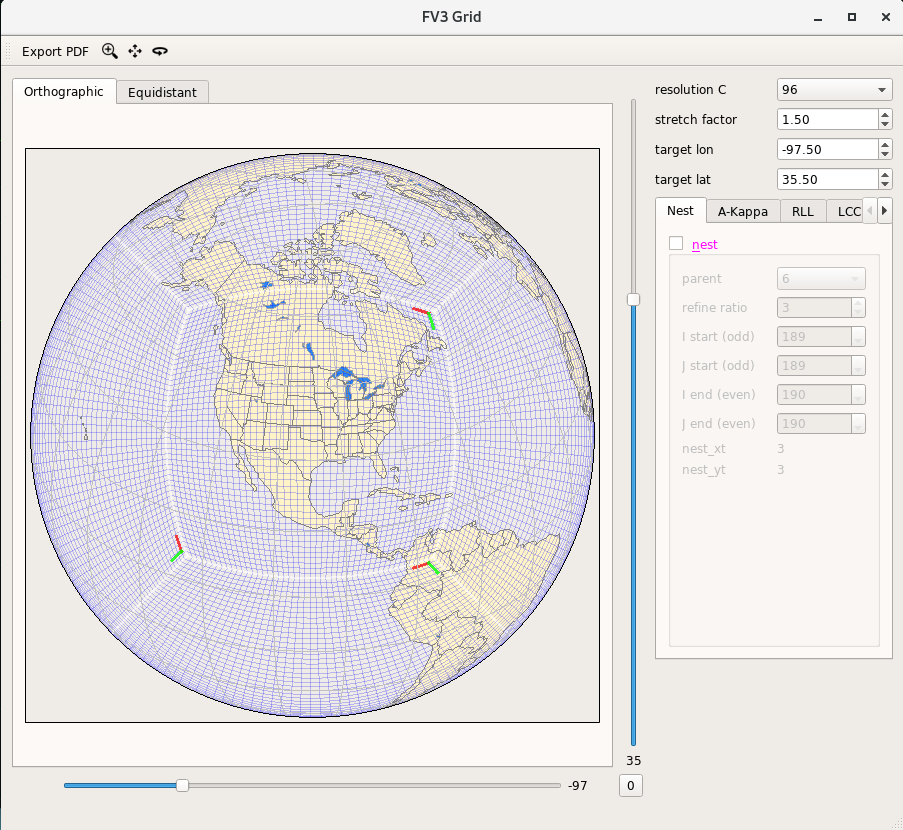
\includegraphics[width=0.6\linewidth]{post_fv3grid_02.png}
  \caption{Change of resolution and stretch factor}
  \label{fig:post_fv3grid_02}
\end{figure}


\item Check the box of `nest' for a regional grid, and set the parameters:

{
\fontsize{10}{12}\selectfont
\begin{longtable}{p{0.12\linewidth} | p{0.8\linewidth} }
\hline
\hline
 Name & Description \\
\hline
 parent & Number of the parent tile where the regional grid is located (=6) \\
 refine ratio & Grid refinement ratio \\
 I start (odd) & Lowest $i$-index of the parent-tile super-grid corresponding to the regional domain\\
 J start (odd) & Lowest $j$-index of the parent-tile super-grid corresponding to the regional domain \\
 I end (even) & Highest $i$-index of the parent-tile super-grid corresponding to the regional domain \\
 J end (even) & Highest $j$-index of the parent-tile super-grid corresponding to the regional domain\\
\hline
\caption{Parameters for a regional grid.}
\label{table:fv3_var_child}
\end{longtable}
}

{\bf Notes)} 
\begin{itemize}
\item To make the domain symmetry along the centerline, `I end'=$2\times$`resolution C'-(`I start'-1), and `J end'=$2\times$`resolution C'-(`J start'-1).
\item The `resolution C' means that the size of the parent tile 6 is \{$2\times$`resolution C'\}$\times$\{$2\times$ `resolution C'\} for the {\it fv3} super-grid or \{`resolution C'\}$\times$\{`resolution C'\} for a general grid.
\end{itemize}

\begin{figure}[ht!]
  \centering
  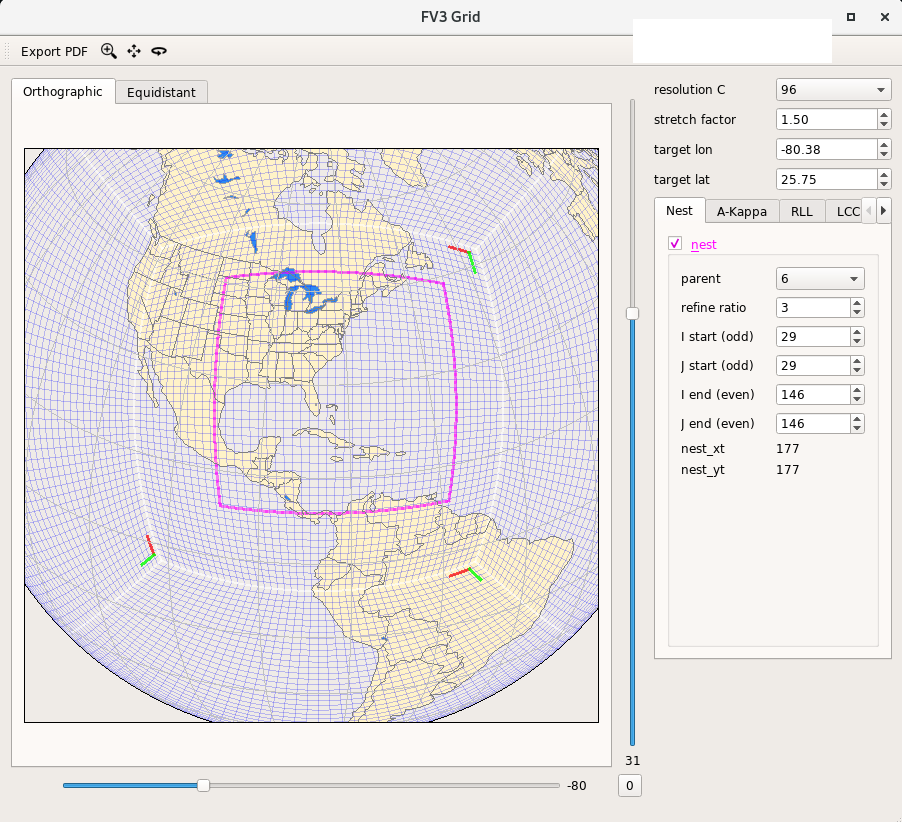
\includegraphics[width=0.6\linewidth]{post_fv3grid_04.png}
  \caption{New regional region of interest}
  \label{fig:post_fv3grid_04}
\end{figure}

\end{enumerate}



%-------------------------------------------
\subsection{Rotated Domain for `output\_grid'}
\label{subsec:fv3grid_rll}

Parameters for plotting extent in `model\_configure' can be found as:

\begin{enumerate}
\item Pop up a display window of {\it fv3grid}:

\begin{itemize}
\item On Hera:
\lstset{language=bash}   
\begin{lstlisting}[frame=trBL]
/scratch2/NCEPDEV/fv3-cam/Dusan.Jovic/dbrowse/fv3grid
\end{lstlisting}
\end{itemize}

\item Set the parameters for Tile 6 in the global and regional domains as shown in Section \ref{subsec:fv3grid_regional}:

\item Click the `RLL' tab on the right of the window, and check the box of `Rotated Lat Lon':

\item Adjust the parameters to put the blue box inside the regional domain in purple:
{
\fontsize{10}{12}\selectfont
\begin{longtable}{p{0.1\linewidth} | p{0.82\linewidth} }
\hline
\hline
Name & Description \\
\hline
 tlm0d & Longitude of the center of the rotated domain (in degrees) \\
 tph0d & Latitude of the center of the rotated domain (in degrees) \\
 wbd & Longitudinal distance from the center to the bottom-left corner of the rotated domain (in degrees)\\
 sbd & Latitudinal distance from the center to the bottom-left corner of the rotated domain (in degrees) \\
\hline
\caption{Parameters for a RLL grid.}
\label{table:fv3grid_RLL}
\end{longtable}
}

\begin{figure}[ht!]
  \centering
  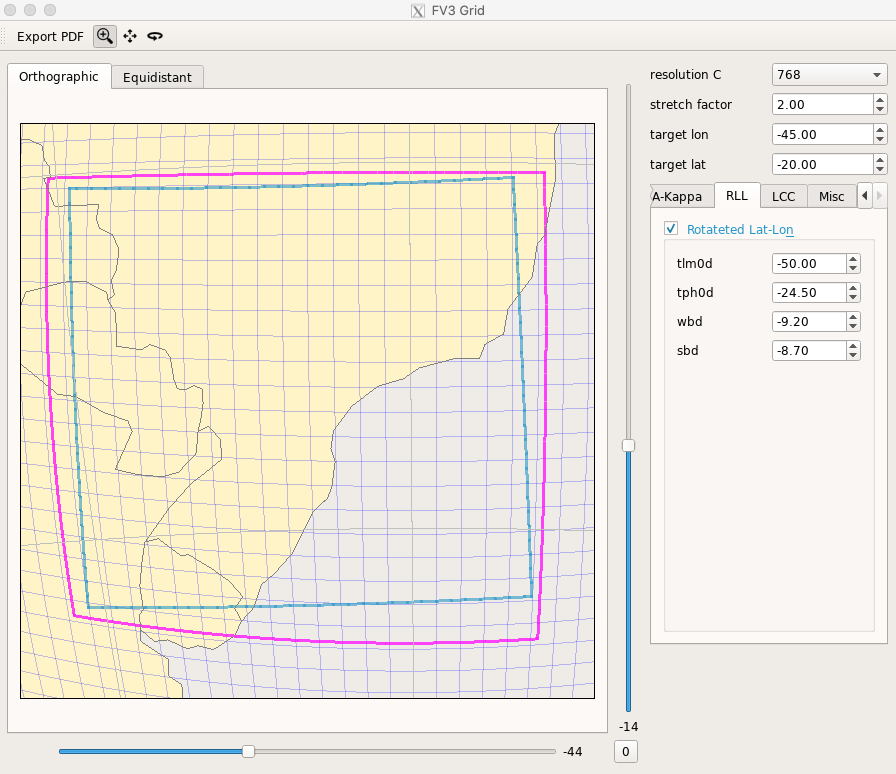
\includegraphics[width=0.6\linewidth]{post_fv3grid_rll.png}
  \caption{Parameters on the rotated grid}
  \label{fig:post_fv3grid_rll}
\end{figure}

{\bf Note)} `tlm0d' and `tph0d' do not need to be the same as `target\_lon' and `target\_lat', respectively. However, it is recommended to make them the same each other.

{\bf Note)} The top-right corner of the rotated domain (box in blue) is automatically set as the same distance from the center as `wbd' and `sbd'.


\end{enumerate}


%-------------------------------------------
\subsection{A--Kappa ($\alpha$--$\kappa$) Domain for an ESG (JP) Grid}
\label{subsec:fv3grid_esg_jp}

\begin{enumerate}

\item Pop up a display window of {\it fv3grid}:

\begin{itemize}
\item On Hera:
\lstset{language=bash}   
\begin{lstlisting}[frame=trBL]
/scratch2/NCEPDEV/fv3-cam/Dusan.Jovic/dbrowse/fv3grid
\end{lstlisting}
\end{itemize}

\item Click the `nest' check box in the `Nest' tap, and set up the GFDL domain for comparison if necessary:
\begin{figure}[ht!]
  \centering
  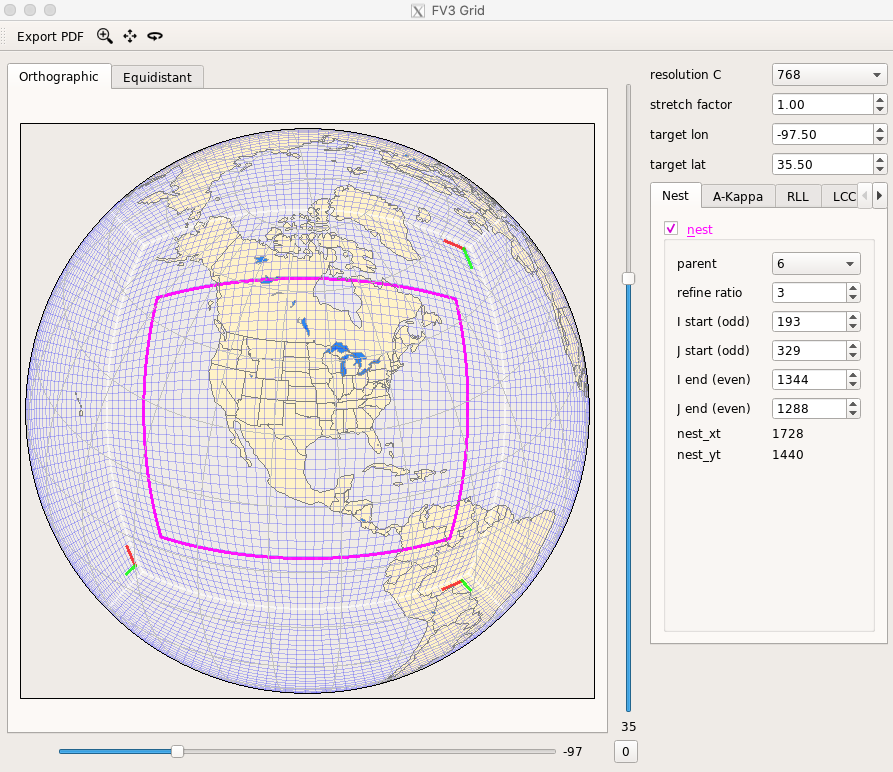
\includegraphics[width=0.6\linewidth]{post_fv3grid_esg1.png}
  \caption{Parameters of a GFDL grid for camparison }
  \label{fig:post_fv3grid_esg1}
\end{figure}

\item Click the `A-Kappa' check box in the `A-Kappa' tap, and adjust the grid parameters for an ESG (JP) grid:
\begin{figure}[ht!]
  \centering
  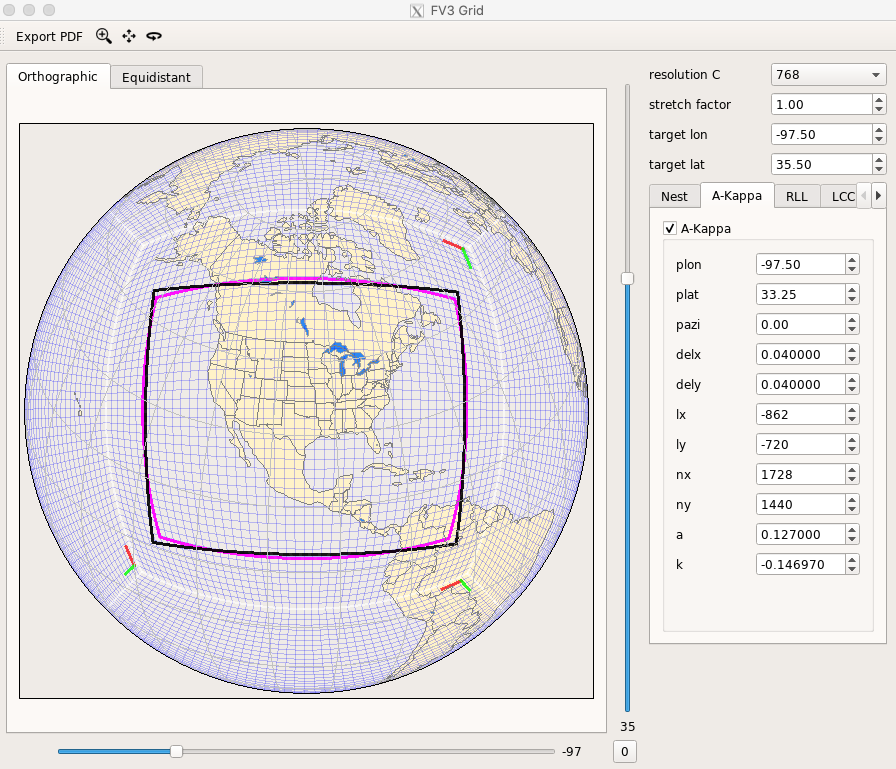
\includegraphics[width=0.6\linewidth]{post_fv3grid_esg2.png}
  \caption{Parameters for an ESG (JP) grid}
  \label{fig:post_fv3grid_esg2}
\end{figure}

\end{enumerate}


%\clearpage


%=================================================== 
\section{Plotting with {\it Python}}               
\label{sec:post_python}

%-------------------------------------------
\subsection{`Natural Earth' Data for Background}

Download shape files:
\lstset{language=bash}   
\begin{lstlisting}[frame=trBL]
www.naturalearthdata.com/downloads/
\end{lstlisting}

The default scale (resolution) of background attributes built in {\it python} is 1:110m. This is good enough for the global domain. However, the medium scale (1:50m) or large scale (1:10m) data are recommended for a regional domain as shown in Figure \ref{fig:ne_scale}.
\begin{itemize}
\item For `Cultural':
\lstset{language=bash}   
\begin{lstlisting}[frame=trBL]
www.naturalearthdata.com/downloads/50m-cultural-vectors/
# Click `Download all 50m cultural themems'
\end{lstlisting}

\begin{figure}[ht!]
  \centering
  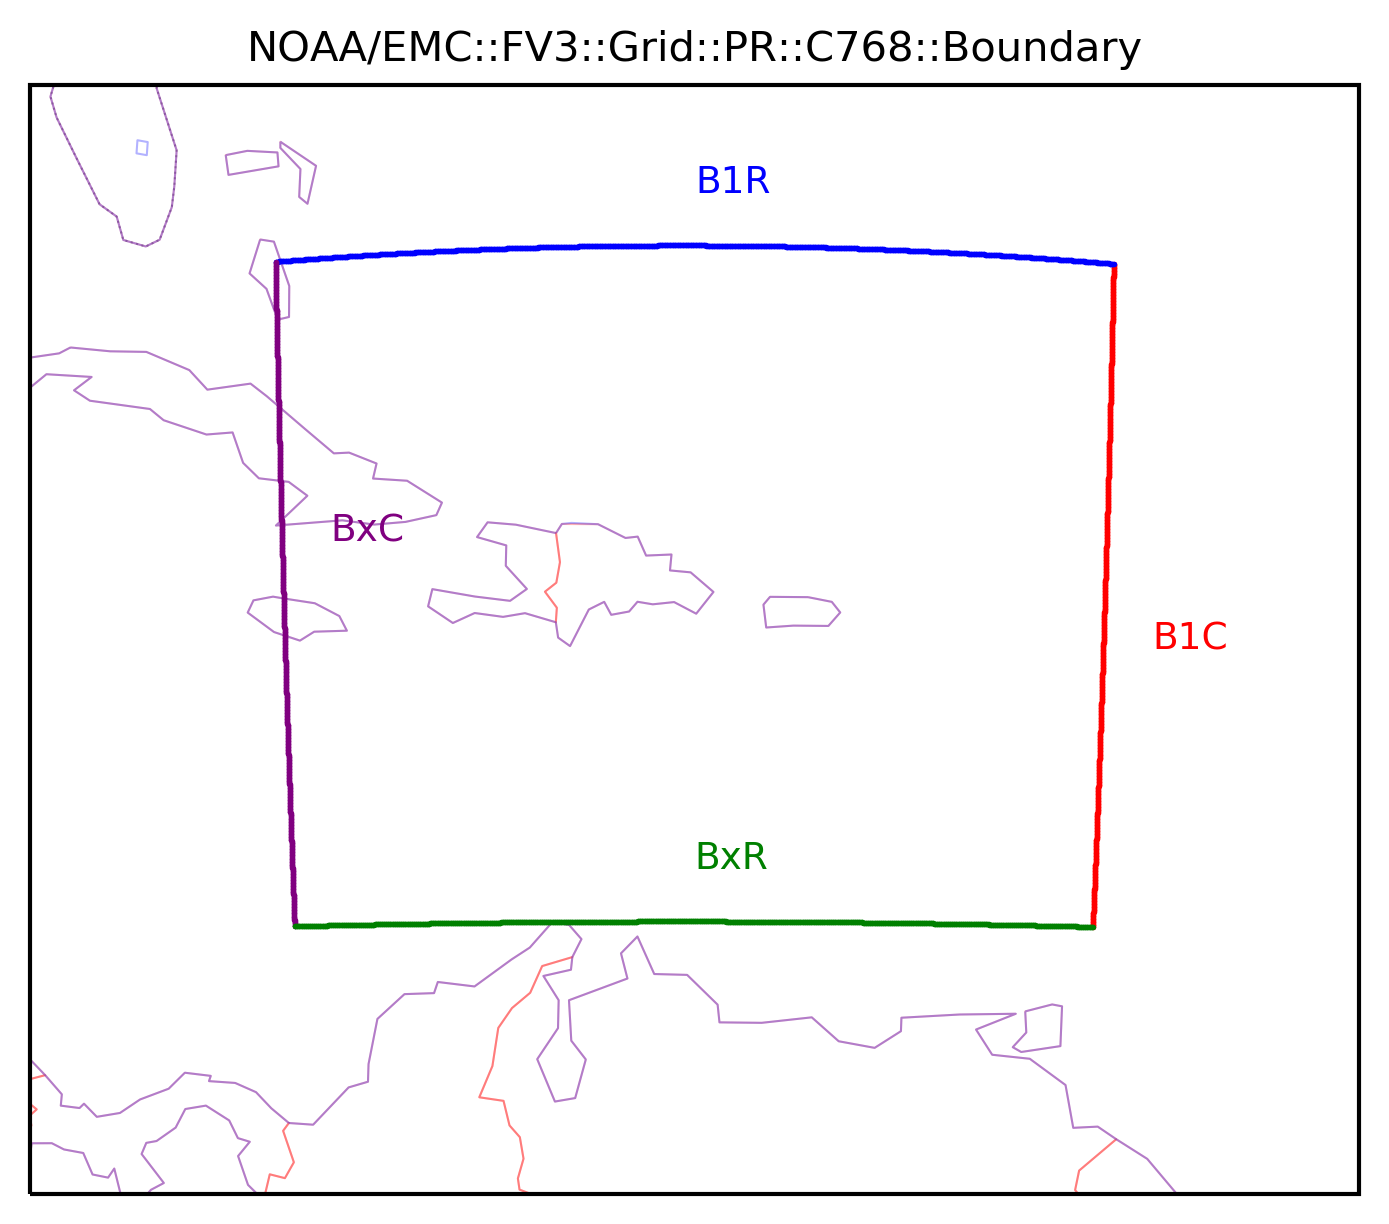
\includegraphics[width=0.4\linewidth]{fv3_pre_grid_PR_C768_bndr_110m.png}
  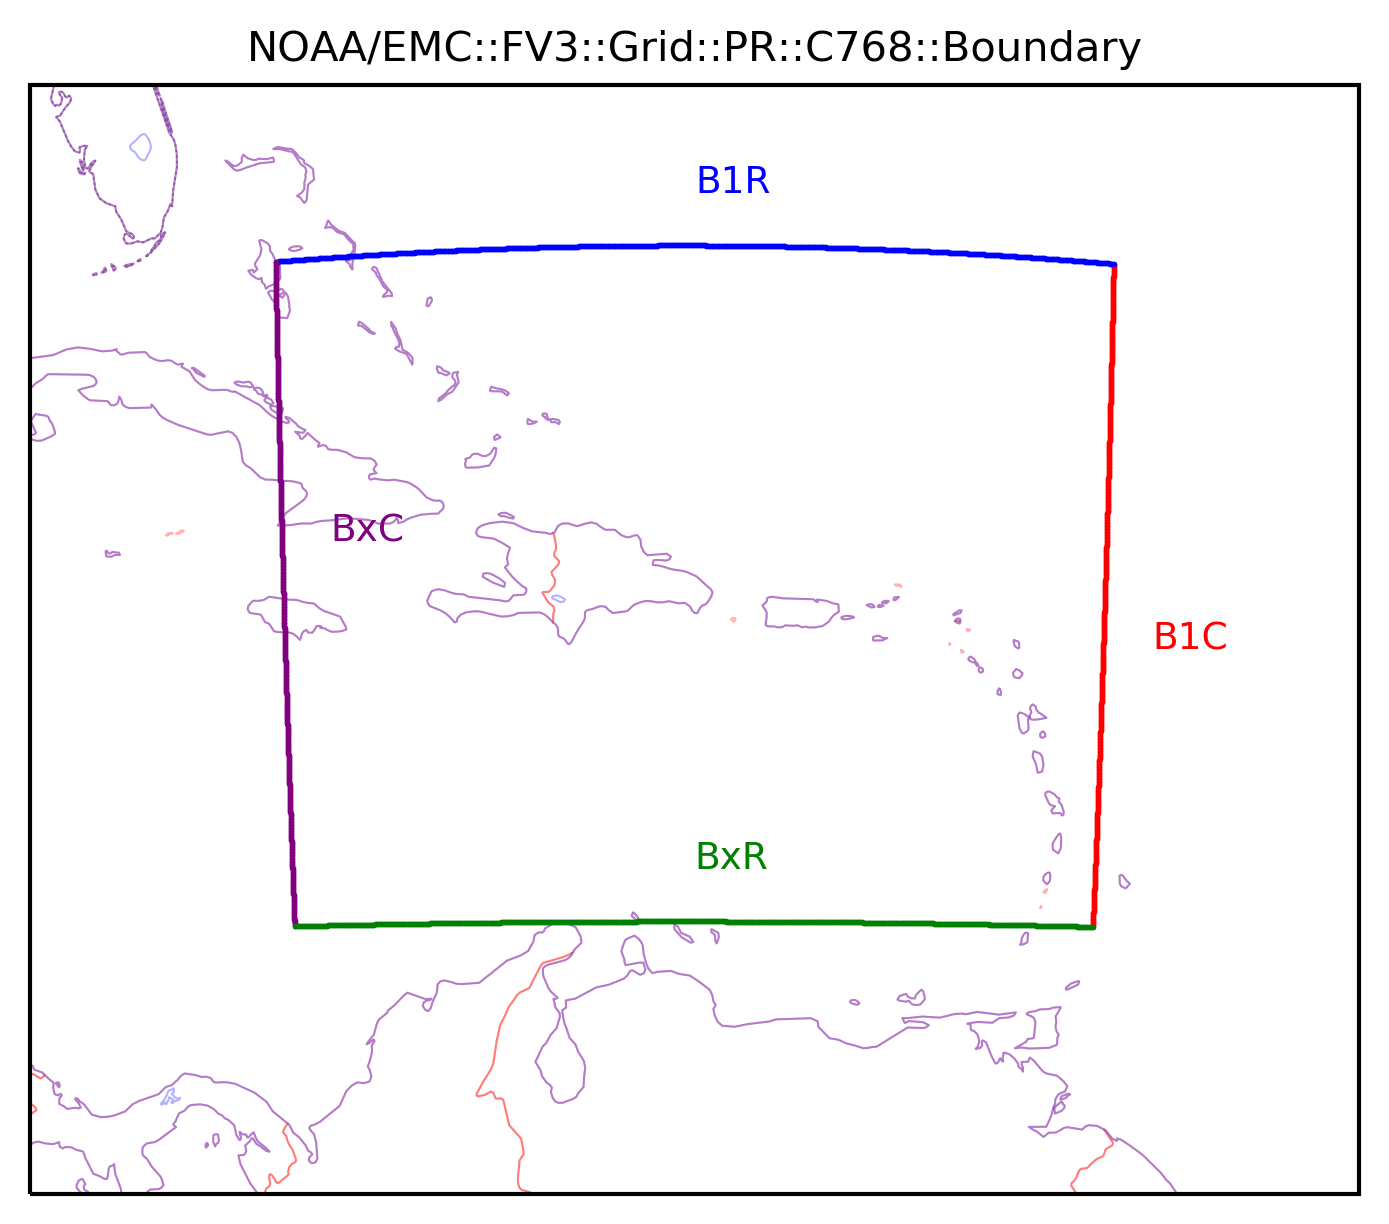
\includegraphics[width=0.4\linewidth]{fv3_pre_grid_PR_C768_bndr_50m.png}
  \caption{Background scales: 1/110$m$ vs. 1/50$m$}
  \label{fig:ne_scale}
\end{figure}

\item For `Physical':
\lstset{language=bash}   
\begin{lstlisting}[frame=trBL]
www.naturalearthdata.com/downloads/50m-physical-vectors/
# Click `download all 50m physical themes'
\end{lstlisting}

\end{itemize}  

Put the files into the specific structures of directories as below:
\lstset{language=bash}   
\begin{lstlisting}[frame=trBL]
$data_dir/shapefiles/natural_earth/physical (or cultural)
\end{lstlisting}

Or, the files can be found as follows: 
\begin{itemize}
\item On Hera:
\lstset{language=bash}   
\begin{lstlisting}[frame=trBL]
/scratch2/NCEPDEV/fv3-cam/Chan-hoo.Jeon/tools/NaturalEarth/
\end{lstlisting}

\item On Orion:
\lstset{language=bash}   
\begin{lstlisting}[frame=trBL]
/home/chjeon/tools/NaturalEarth/
\end{lstlisting}

\end{itemize}


Set the path in the script:
\begin{itemize}
\item On Hera:
\lstset{language=bash}   
\begin{lstlisting}[frame=trBL]
cartopy.config[`data_dir']=`/scratch2/NCEPDEV/fv3-cam/Chan-hoo.Jeon/tools/NaturalEarth'
\end{lstlisting}

\item On Orion:
\lstset{language=bash}   
\begin{lstlisting}[frame=trBL]
cartopy.config[`data_dir']=`/home/chjeon/tools/NaturalEarth'
\end{lstlisting}

\end{itemize}



%--------------------------------------------------------------------------------------------
\subsection{Cartopy Background Image}

Cartopy provides the `background\_img()' method to add background images in a convenient way. You can specify custom background images.

\begin{enumerate}
\item Download background images such as Natural Earth data and put them in the specific directory.

\item Set up the environment variable for the path of the directory that contains the background images:
\lstset{language=bash}   
\begin{lstlisting}[frame=trBL,basicstyle=\scriptsize]
{
os.environ["CARTOPY_USER_BACKGROUNDS"]="/scratch2/NCEPDEV/fv3-cam/Chan-hoo.Jeon/tools/NaturalEarth/raster_files"
}
\end{lstlisting}


\item  The arguments of `name' and `resolution' for the `background\_img()' are specified in the configuration file `images.json' that should be located in the above directory. An example of the `images.json' file is as follows: 

\lstset{language=bash}   
\begin{lstlisting}[frame=trBL,basicstyle=\scriptsize]
{
    "NE": {
    "__comment__": "Natural Earth raster file",
    "__source__": "www.naturalearthdata.com/downloads",
    "__projection__": "PlateCarree",
    "high": "NE1_50M_SR_W.tif"}
}
\end{lstlisting}

\begin{figure}[ht!]
  \centering
  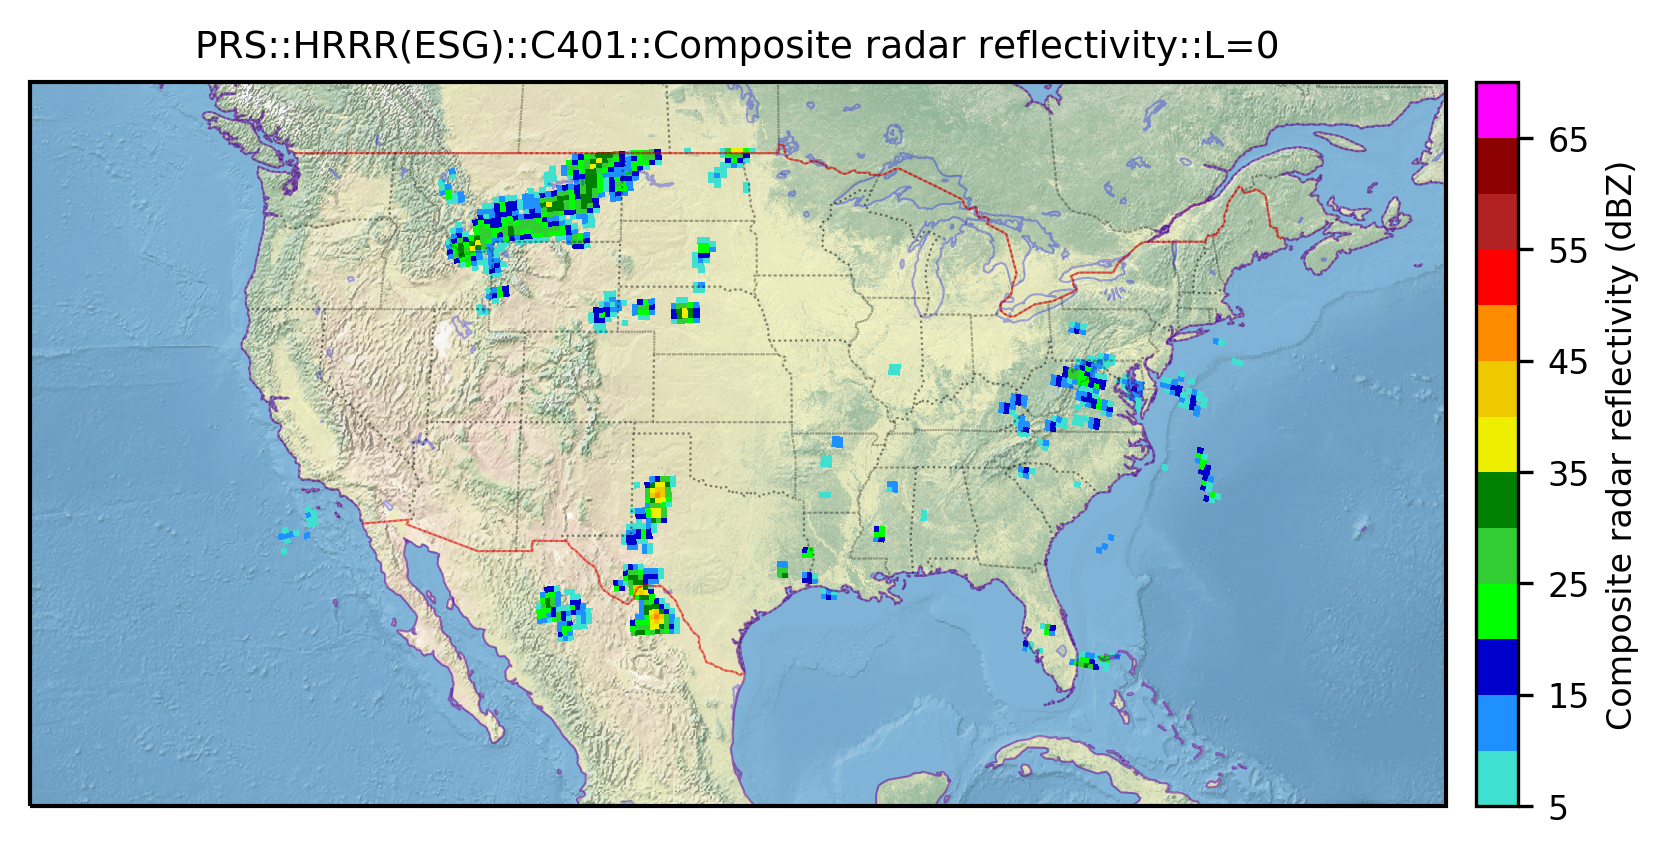
\includegraphics[width=0.7\linewidth]{fv3_out_prs_HRRR_esg_C401_refc_unknown_L001.png}
  \caption{Background image: Natural Earth data}
  \label{fig:py_background_img}
\end{figure}

\item Call `background\_img()' in the script as follows:
\lstset{language=bash}   
\begin{lstlisting}[frame=trBL]
ax.background_img(name=`NE', resolution=`high')
\end{lstlisting} 

\end{enumerate}


{\bf Note)} A low-resolution background image can be easily called by `stock\_img()' in a script.



%---------------------------------------------------------------------------------------------
\subsection{Modules}

If a HPC, such as Hera, provides a module of `Anaconda/Miniconda', you can load modules for running python scripts as follows:
\begin{itemize}
\item On Hera:
\lstset{language=bash}   
\begin{lstlisting}[frame=trBL]
module load intel
module use -a /contrib/anaconda/modulefiles
module load anaconda/latest
\end{lstlisting}
\end{itemize}
{\bf Note)} If `Miniconda (or Anaconda)' is installed in the home directory, you do not need to load the above modules for running post-processing python scripts. \\

To import `pygrib' on WCOSS, you should modules as follows:
\begin{itemize}
\item WCOSS Dell:
\lstset{language=bash}   
\begin{lstlisting}[frame=trBL]
module load ips/19.0.5.281
module load impi/19.0.5
module load grib_util/1.1.1
module load python/3.6.3
module use -a /u/Benjamin.Blake/modulefiles
module load python3/test
export GRIB_DEFINITION_PATH=/usrx/local/nceplibs/dev/lib/grib_api/share/grib_api/definitions
\end{lstlisting}

\end{itemize}


%--------------------------------------------------------------------------------------
\subsection{Installation of Miniconda (Anaconda)}

If a HPC, such as Orion, does not provide a module of `Anaconda' for python packages, you need to install either `Miniconda' or `Anaconda' in your home/work directory.

\begin{enumerate}

\item Download the installer from the Miniconda repository:
\lstset{language=bash}   
\begin{lstlisting}[frame=trBL]
wget https://repo.anaconda.com/miniconda/Miniconda3-latest-Linux-x86_64.sh
\end{lstlisting}

\item Verify the installer hashes:
\lstset{language=bash}   
\begin{lstlisting}[frame=trBL]
sha256sum Miniconda3-latest-Linux-x86_64.sh
# Compare the hash code to that on the website (`https://conda.io/projects/conda/en/latest/user-guide/install/linux.html')
\end{lstlisting}


\item Install Miniconda:
\lstset{language=bash}   
\begin{lstlisting}[frame=trBL]
bash Miniconda3-latest-Linux-x86_64.sh
(enter)
(space bar)
(yes)
(enter) or specify the location to be installed ({$CONDA_DIR}).
(enter)
\end{lstlisting}

\item Update the path
\lstset{language=bash}   
\begin{lstlisting}[frame=trBL]
vim ~/.bashrc
# insert
export PATH={$CONDA_DIR}/miniconda3/bin:$PATH
# close the `.bashrc' file
source ~/.bashrc
\end{lstlisting}

\item Test the installation
\lstset{language=bash}   
\begin{lstlisting}[frame=trBL]
conda list
\end{lstlisting}

\item Install the packages required for running the post-processing python scripts:
\lstset{language=bash}   
\begin{lstlisting}[frame=trBL]
conda install cartopy
conda install xarray
conda install netcdf4
conda install dask
conda install -c conda-forge pygrib
\end{lstlisting}

\end{enumerate}



%--------------------------------------------------------------------------------------
\subsection{Python Scripts on GitHub}
\label{subsec:python_script_github}

The python scripts described in this section can be cloned from GitHub as:
\lstset{language=bash}   
\begin{lstlisting}[frame=trBL]
git clone https://github.com/chan-hoo/FV3LAM_plot_python.git
\end{lstlisting}

The list of the scripts in the above repository is shown in Table \ref{table:python_script_list}. The scripts are based on Python 3.7, and Python libraries of `matplotlib', `xarray', and `cartopy' are applied.

{
\fontsize{10}{12}\selectfont
\begin{longtable}{ p{0.25\linewidth} | p{0.6\linewidth} }
\hline
\hline
 Script name & Description \\
\hline
 modules\_hera & Module list for Anaconda on Hera \\
 modules\_wcoss\_dell & Module list for pygrib on the WCOSS Dell \\
 plot\_fv3lam\_grid\_oro.py & Grid and orography files \\
 plot\_fv3lam\_gridonly.py & Grid file alone \\
 plot\_fv3lam\_static.py & Regional static field files \\
 plot\_fv3lam\_fixam.py & Global static field files \\
 plot\_fv3lam\_icbc.py & Time-dependent IC/LBC fields \\
 plot\_fv3lam\_icsfc.py & Initial surface climatology fields \\
 plot\_fv3lam\_co2his.py & Historical CO$_2$ data \\
 plot\_fv3lam\_gridspec.py & Output `grid\_spec.nc' file \\
 plot\_fv3lam\_atmstat.py & Output `atmos\_static.nc' file \\
 plot\_fv3lam\_his2d\_bndr.py & Boundary regions of output `fv3\_history2d.nc' file \\
 plot\_fv3lam\_dynf.py & Output `dynffXXX.nc' file \\
 plot\_fv3lam\_phyf.py & Output `phyfXXX.nc' file \\
 plot\_fv3lam\_bgrd3d.py & Output `BGRD3D' GRIB2 file \\
 plot\_fv3lam\_bgdawp.py & Output `BGDAWP' GRIB2 file \\ 
 plot\_fv3lam\_comp2f.py & Comparison of two NetCDF (GRIB2) files \\
 plot\_fv3lam\_mrms.py & MRMS radar data for reflectivity \\
 plot\_fv3lam\_ani\_comref.py & Animation of hourly comparison of GRIB2 and radar data \\
 plot\_fv3lam\_grb2his.py & Time-history plot of max. total precipitation/ reflectivity from BGDAWP GRIB2 files \\
\hline
\caption{Python scripts for plotting input and output files.}
\label{table:python_script_list}
\end{longtable}
}



%--------------------------------------------------------------------------------------
\subsection{Grid and Orography}
\label{subsec:python_grid_oro}

The python script `plot\_fv3lam\_grid\_oro.py' creates figures for grid and orography in a regional domain. \\

{\bf Note)} If you want to plot the grid file without the orography file, you can use another script `plot\_ fv3lam\_grid.py'.

\begin{enumerate}
\item Input files
\begin{itemize}
\item gird.tile7.halo4.nc (grid)
\item oro\_data.tile7.halo4.nc (orography)
\end{itemize}
\item Output files
\begin{itemize}
\item fv3lam\_grid.png (grid)
\item fv3lam\_grid\_bndr.png (boundary of domain)
\item fv3lam\_grid\_dxy.png (cell size)
\item fv3lam\_grid\_crnr\_RXCX.png (grid at the four corners)
\item fv3lam\_orog\_\{variables\}.png  (orography variables)
\end{itemize}
\item Run on HPC

\lstset{language=bash}   
\begin{lstlisting}[frame=trBL]
# Check Input and Output paths and names
vim plot_fv3lam_grid_oro.py
# Run the script
python3 plot_fv3sar_grid_oro.py
\end{lstlisting}

{
\fontsize{10}{12}\selectfont
\begin{longtable}{p{0.22\linewidth} | p{0.65\linewidth} }
\hline
\hline
 Name & Description \\
\hline
 machine & HPC machine for plotting \\
 dnm\_data & Path to the directory where the grid file is located   \\
 dnm\_orog & Path to the directory where the orography file is located \\
 fnm\_in\_grid & File name of the input grid file \\
 fnm\_in\_orog & File name of the input orography file \\
 n\_skip & Number of grid points in lows/column skipped for plotting \\
 out\_fig\_dir & Path to the directory where output files are created \\
 out\_grd\_title & Basic title in the output grid files \\
 out\_grd\_fname & Basic file name of the out grid files \\
 out\_orog\_title\_base & Basic title in the output orography files \\
 out\_orog\_fname\_base & Basic file name of the out orography files \\
 orog\_vars & Variable names plotted in the orography file \\
 cmap\_range\_grd & Colormap range option (`symmetry', `round', `fixed') \\
 back\_res & Resolution of background natural earth data (`50m' or `110m') \\
\hline
\caption{Namelist in the script for plotting gird and orography.}
\label{table:fv3_var_grid_oro}
\end{longtable}
}

\item Output: \\
For example, the following files for the CONUS (C96) domain are created in the output directory:
\begin{enumerate}
\item Grid points for every `n\_skip' rows/columns (`fv3\_grid\_CONUS\_C96.png')
\begin{itemize}
\item For a clear view, grid points are shown at every `n\_skip'-th row and column from ($i=2,j=2$) for the super-grid of {\it fv3} in red, and ($i=1,j=1$) for the typical grid such as the grid of orography in green. This is because the super-grid includes not only a grid point at the center of a cell but also grid points at the corner of a cell.
\item Default values of `n\_skip': 10 for `CONUS', 50 for `AK', 20 for `PR', and 50 for others. 
\end{itemize}


\item Grid points along the boundary (`fv3\_gird\_CONUS\_C96\_bndr.png')
\begin{itemize}
\item This figure only shows the grid points along the four boundaries.
\begin{enumerate}
\item B1C: Along the first column ($j=1$) in red
\item B1R: Along the first row ($i=1$) in blue
\item BxC: Along the last column ($j=x$) in purple
\item BxR: Along the last row ($i=x$) in green
\end{enumerate}
\end{itemize}

\begin{figure}[ht!]
  \centering
  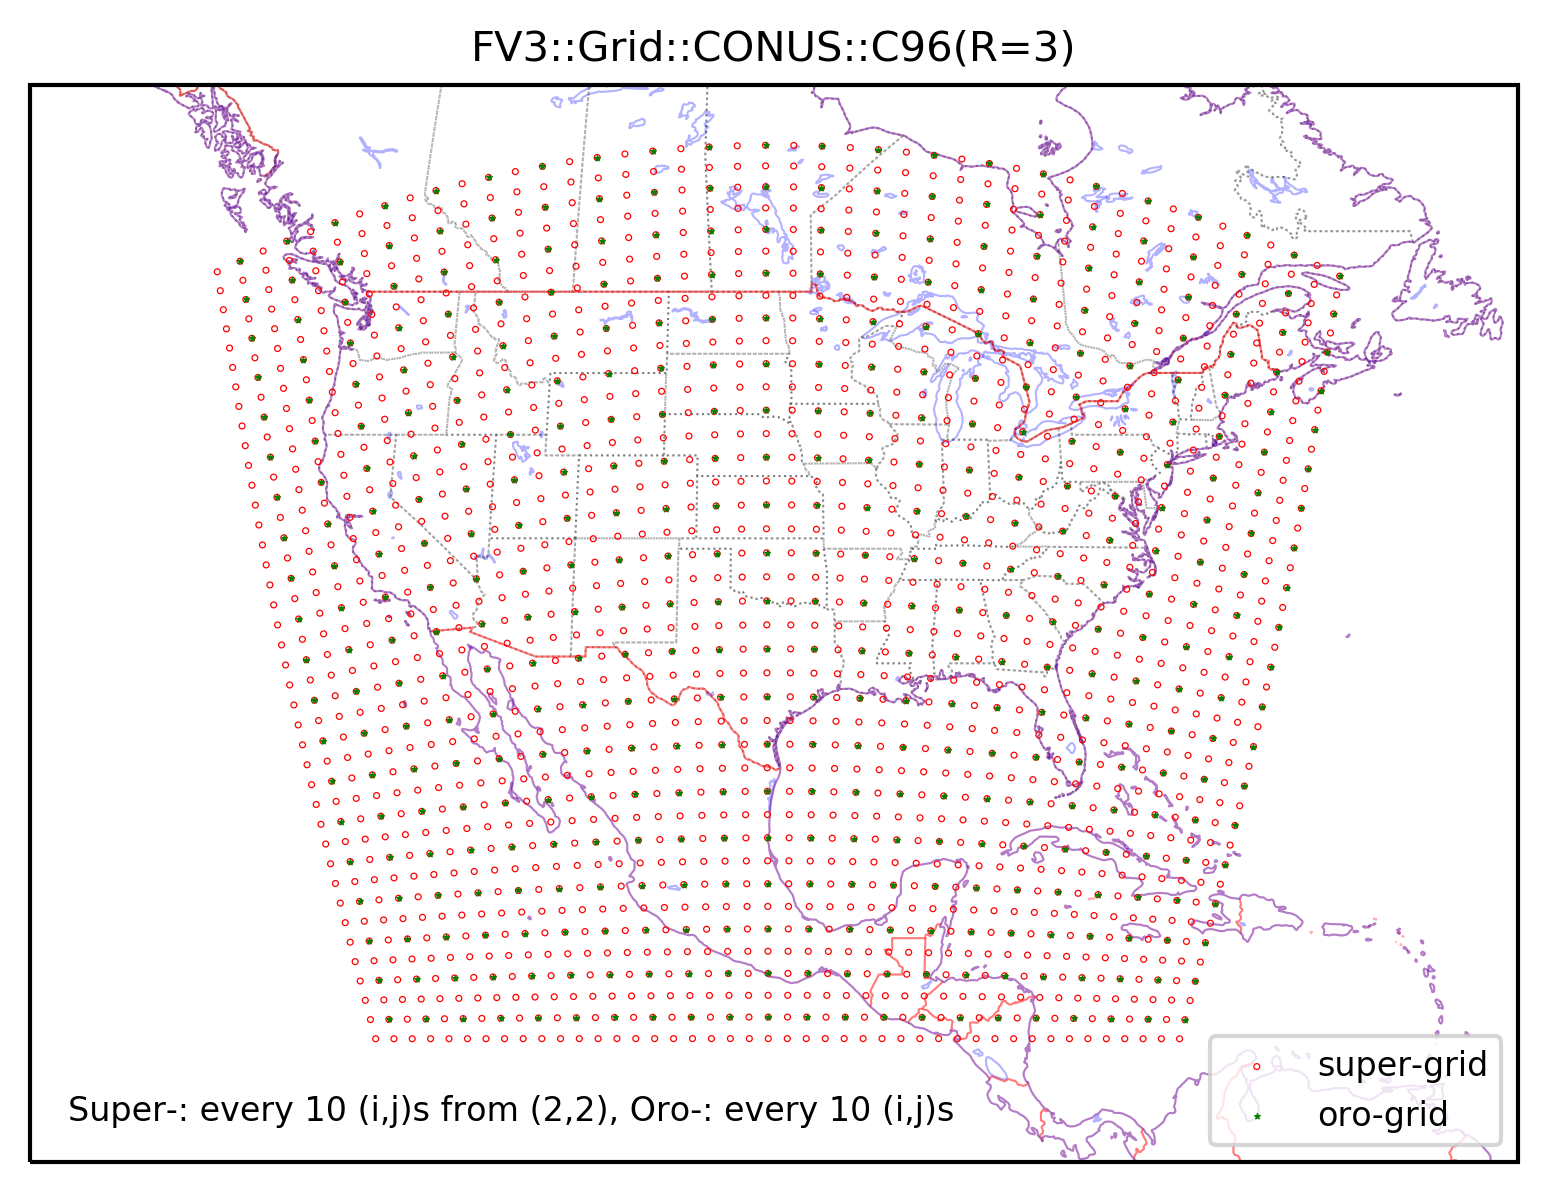
\includegraphics[width=0.49\linewidth]{fv3_grid_CONUS_C96.png}
  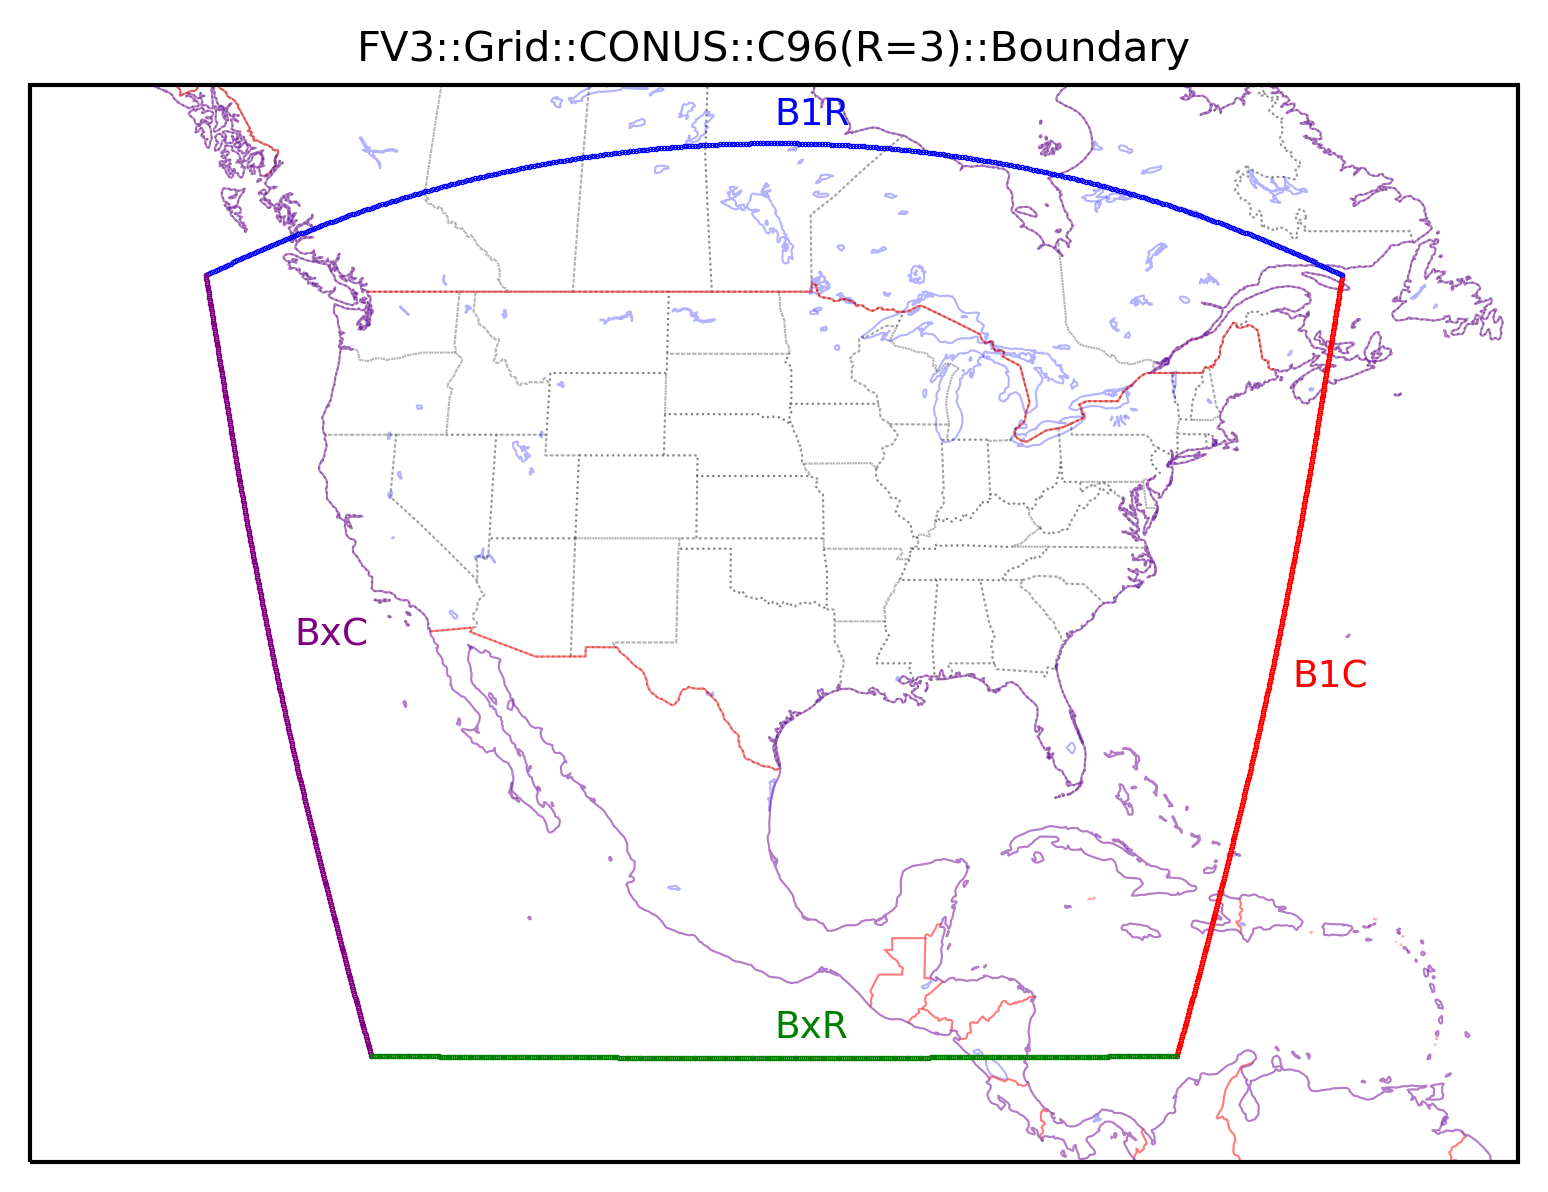
\includegraphics[width=0.49\linewidth]{fv3_grid_CONUS_C96_bndr.png}  
  \caption{Grid points at every 10 rows and columns, and along boundaries}
  \label{fig:py_grid_npts}
\end{figure}

\item Grid cell sizes (`fv3\_grid\_CONUS\_C96\_dxy.png')

\begin{figure}[ht!]
  \centering
  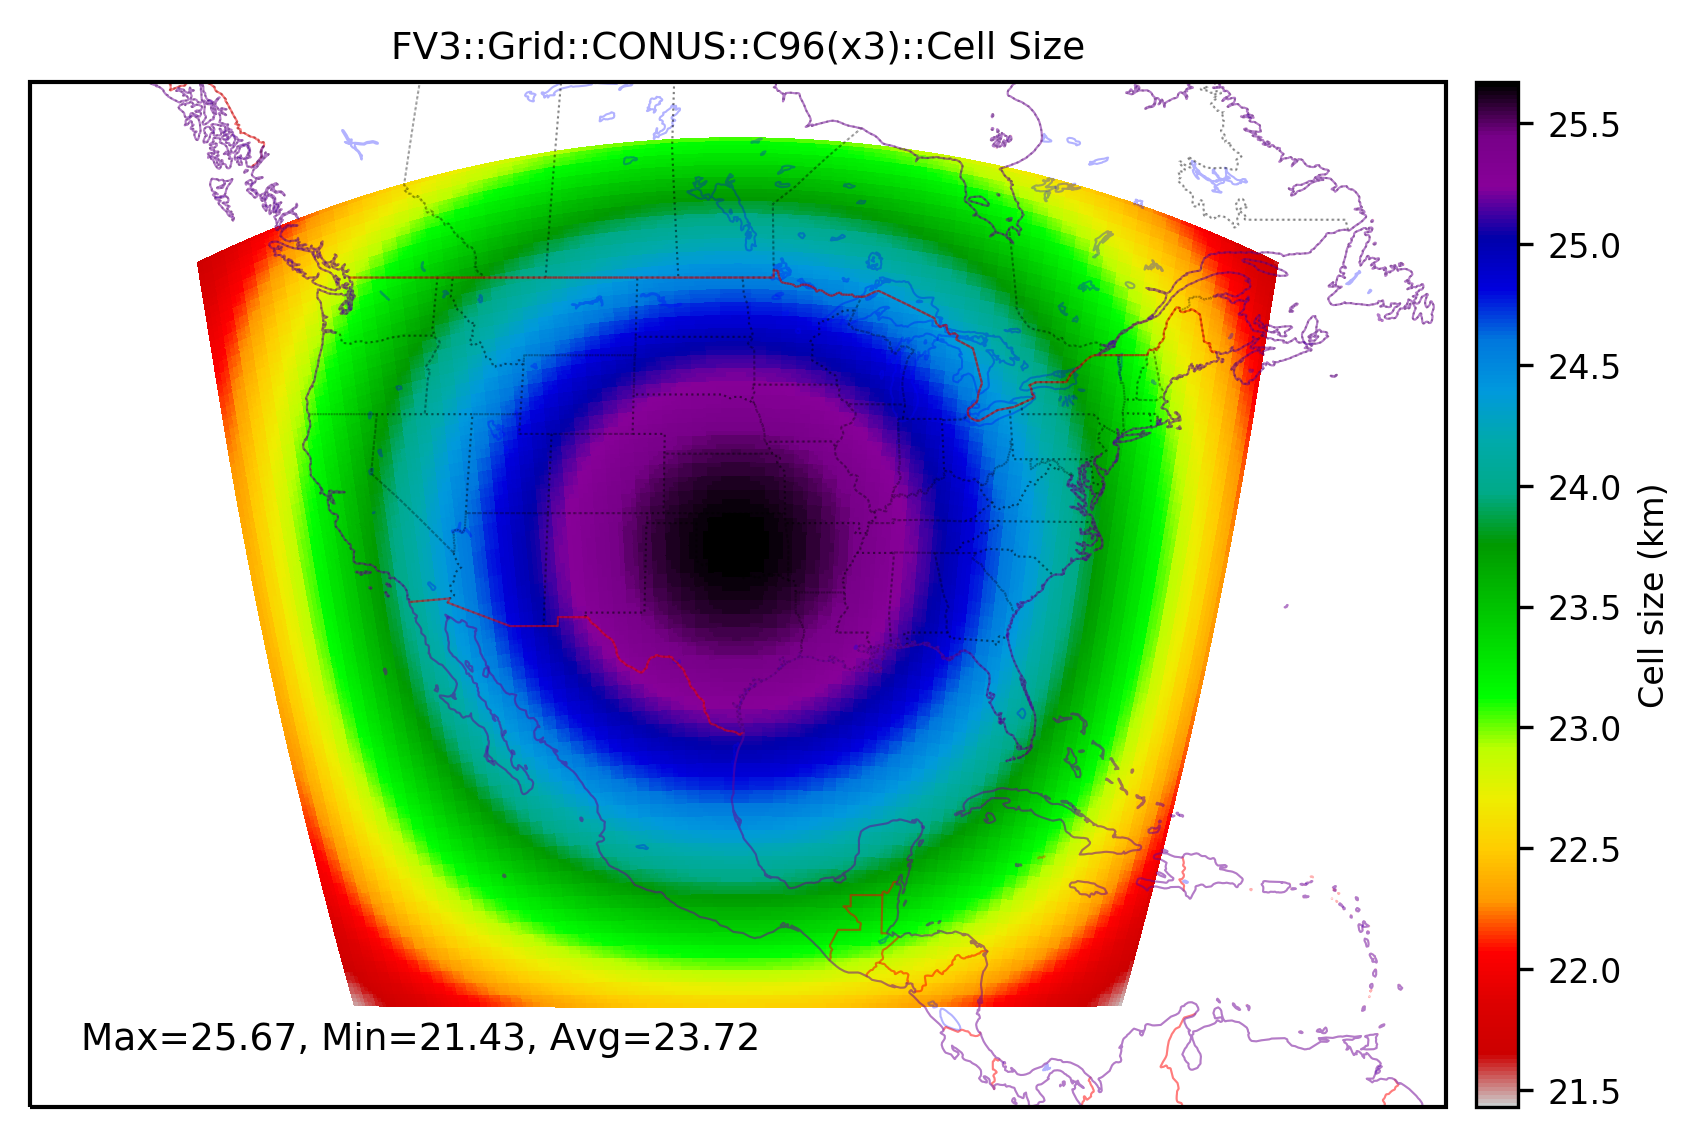
\includegraphics[width=0.65\linewidth]{fv3_grid_CONUS_C96_dxy.png}
  \caption{Cell size}
  \label{fig:py_grid_csize}
\end{figure}


\item Grid points at the four corners  (`fv3\_grid\_CONUS\_C96\_crnr\_[X].png')
\begin{itemize}
\item Each corner has a separate plot: R1C1, R1Cx, RxC1, and RxCx.
\begin{enumerate}
\item R1C1: Around the corner ($i=1, j=1$), intersection between B1R and B1C
\item R1Cx: Around the corner ($i=1, j=x$), intersection between B1R and BxC
\item RxC1: Around the corner ($i=x, j=1$), intersection between BxR and B1C
\item RxCx: Around the corner ($i=x, j=x$), intersection between BxR and BxC
\end{enumerate}
\item Each figure shows 30 rows/columns by the default. It can be adjusted by modifying the value of `N\_crn' in the script. 
\item They plot both the {\it fv3} super-grid and the typical grid (`oro-grid' on the figures).
\end{itemize}


\item Orography (raw and filtered)

\begin{figure}[ht!]
  \centering
  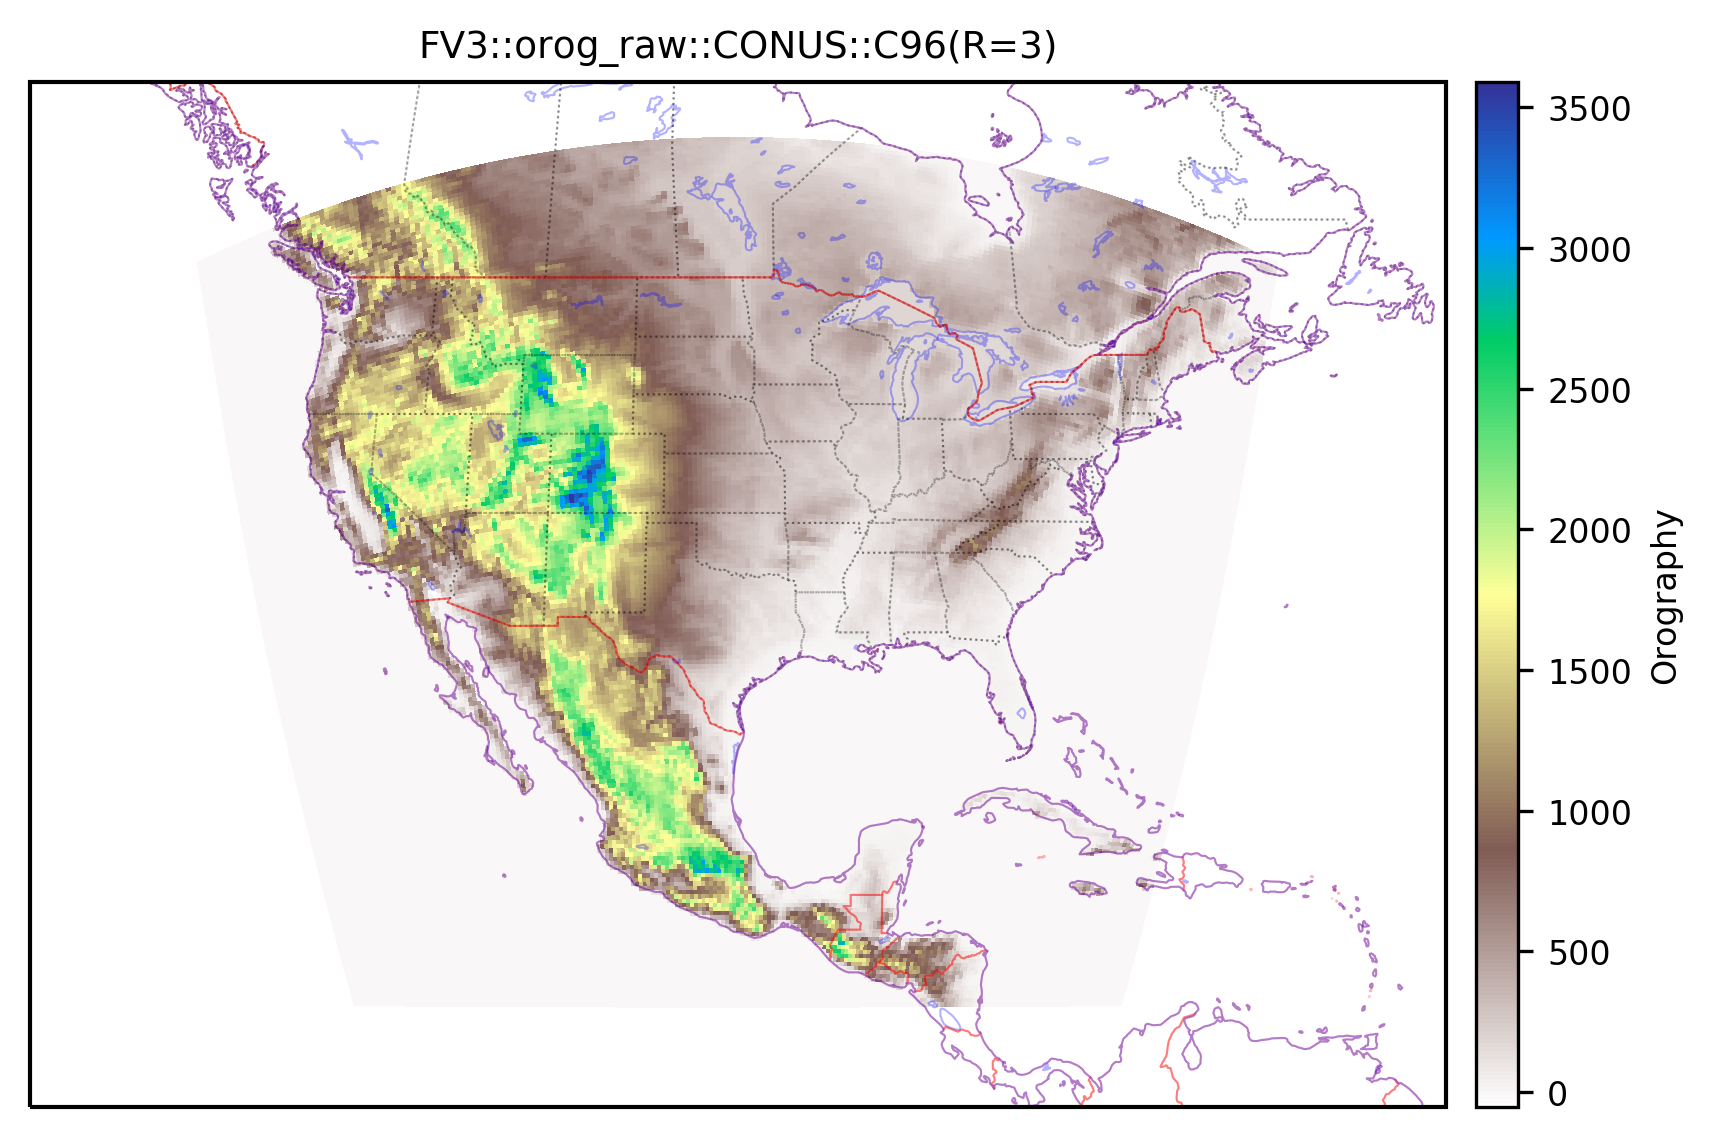
\includegraphics[width=0.48\linewidth]{fv3_orog_CONUS_C96_orog_raw.png}
  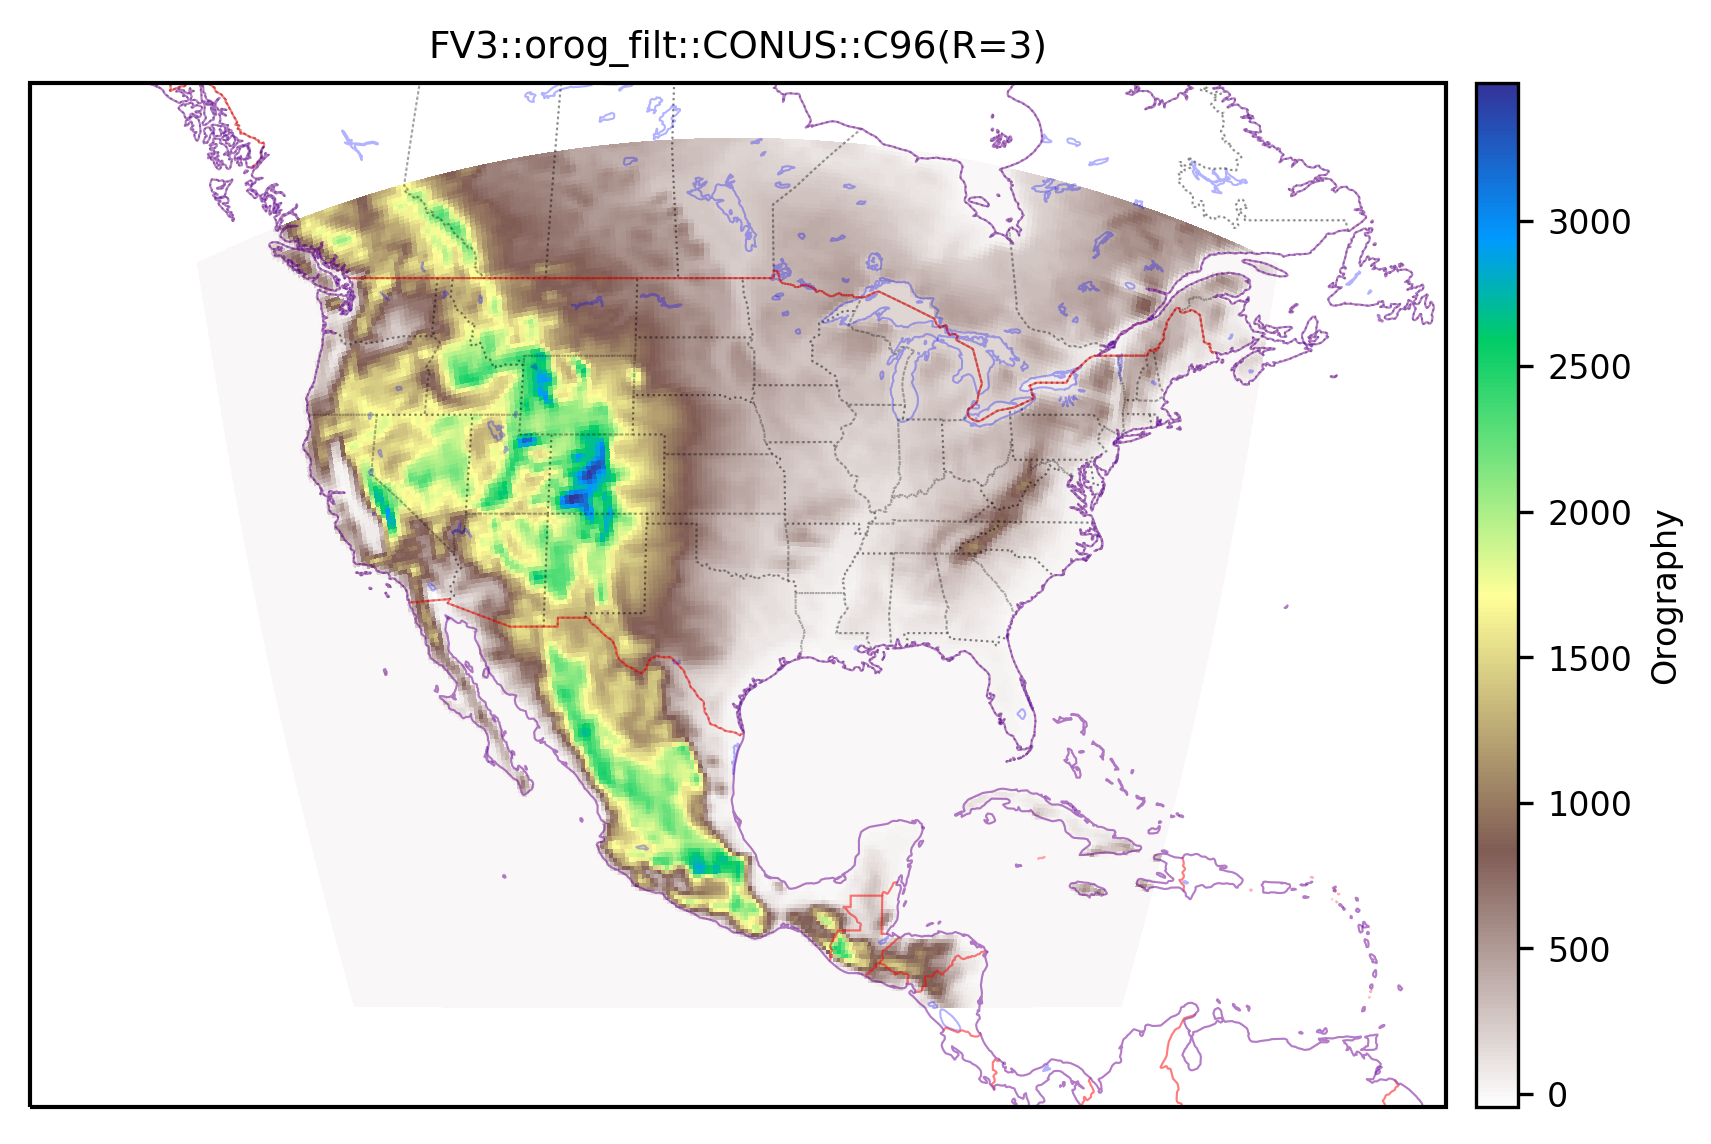
\includegraphics[width=0.48\linewidth]{fv3_orog_CONUS_C96_orog_filt.png}
  \caption{Orography}
  \label{fig:py_orog}
\end{figure}


\item Sea-land mask (sea:0, land:1), and land fraction

\begin{figure}[ht!]
  \centering
  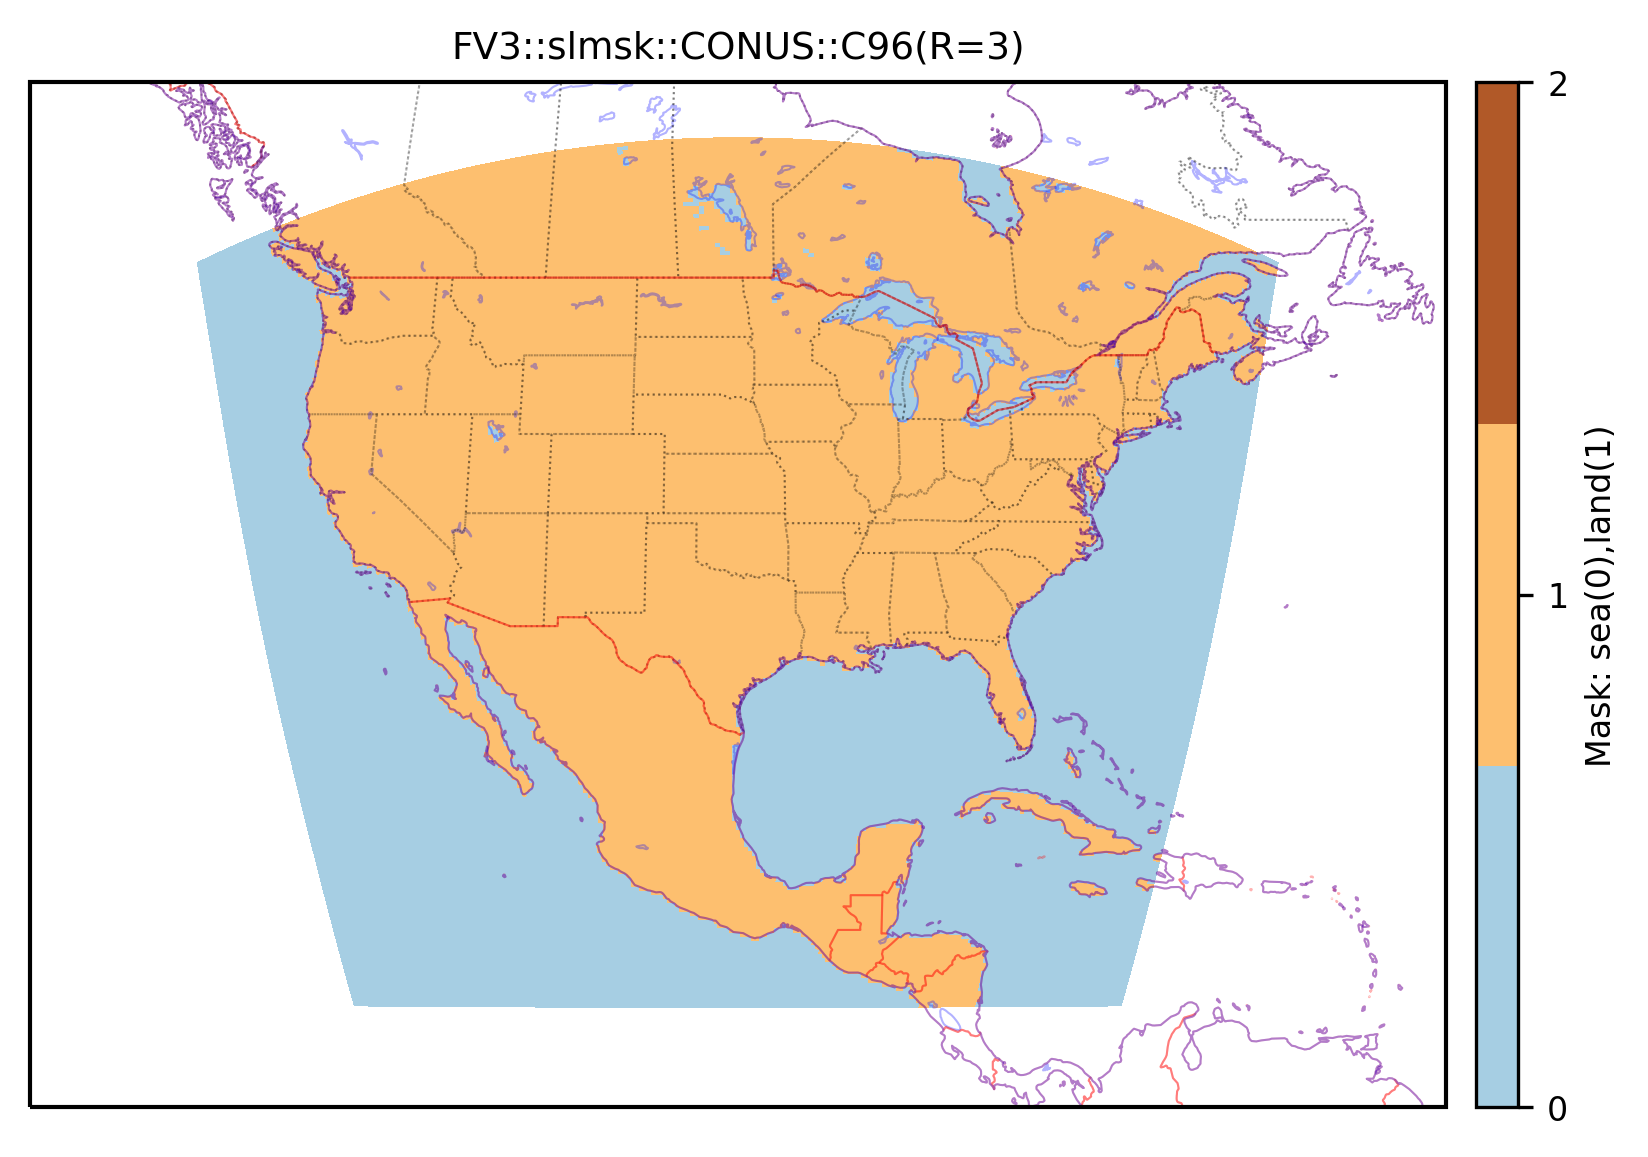
\includegraphics[width=0.48\linewidth]{fv3_orog_CONUS_C96_slmsk.png}
  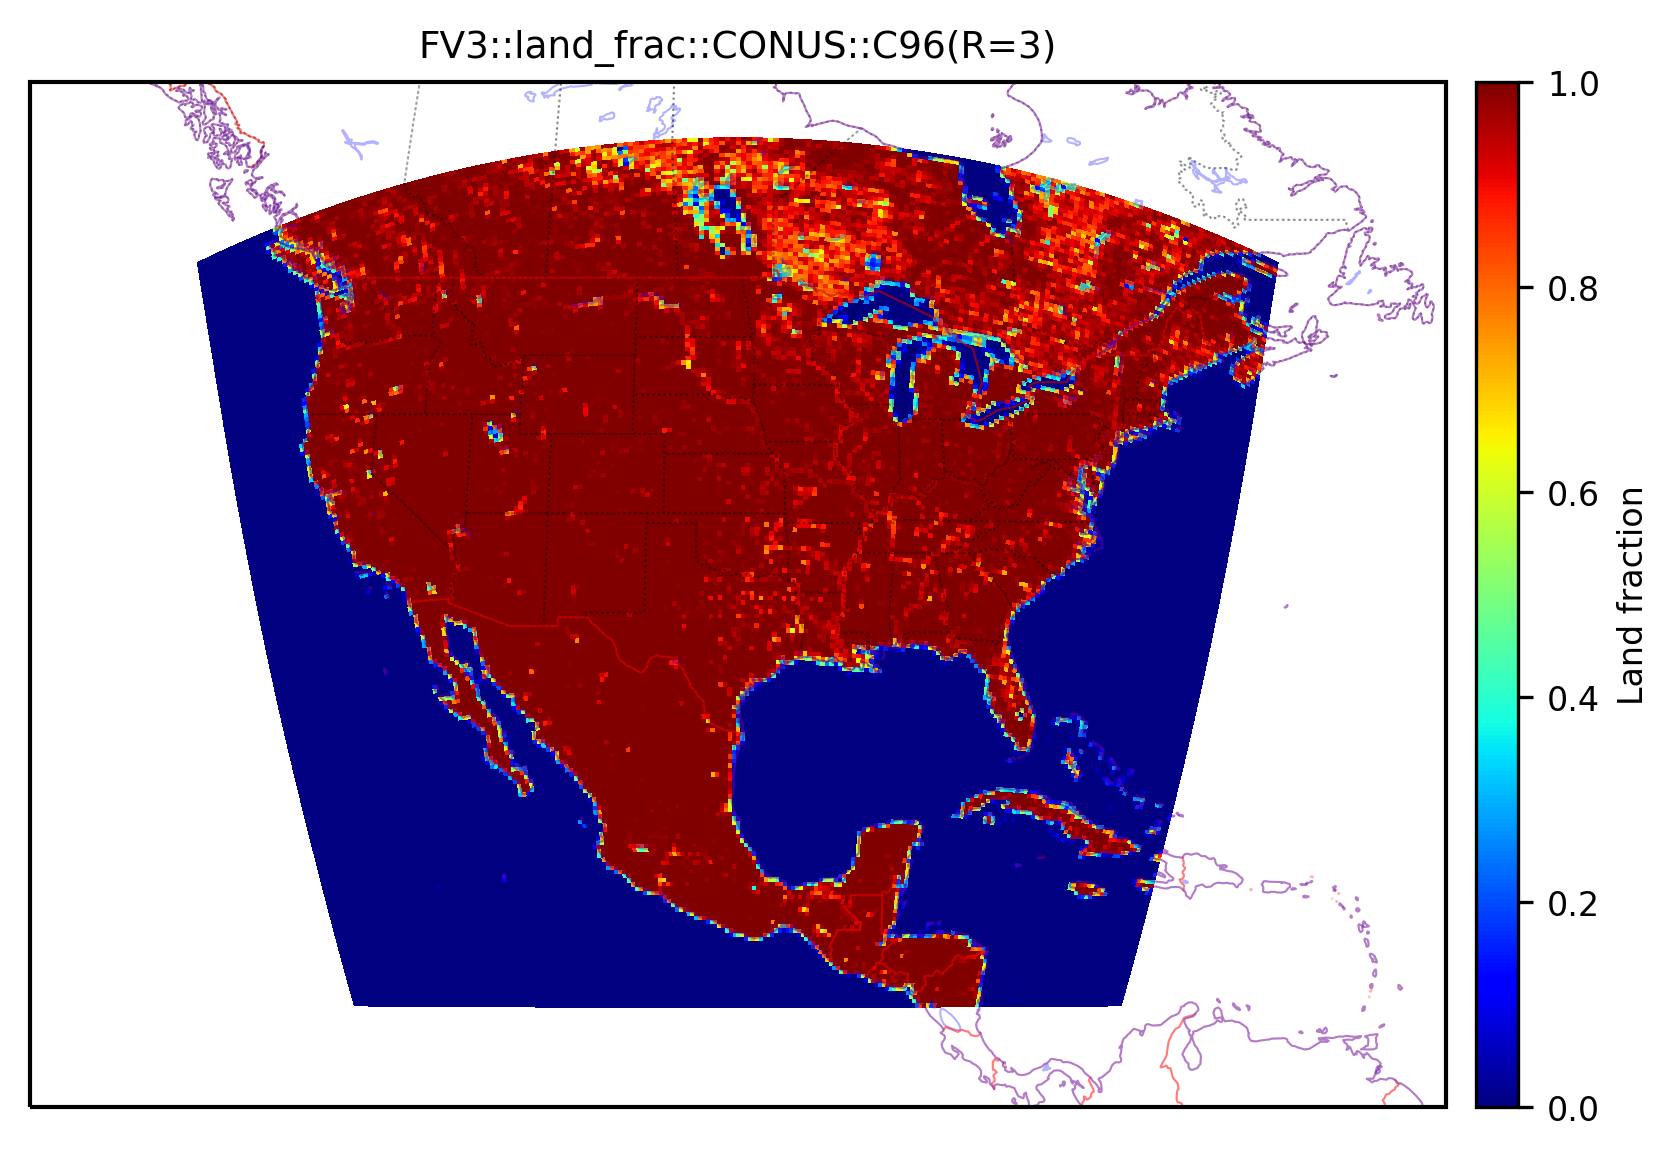
\includegraphics[width=0.48\linewidth]{fv3_orog_CONUS_C96_land_frac.png}
  \caption{Sea-land mask, and land fraction}
  \label{fig:py_mask}
\end{figure}

\end{enumerate}

{\bf Note)} The variables in the input orography file (`C\{res\}\_oro\_data.tile7.halo4.nc') are listed in Table \ref{table:var_oro_output}.

\end{enumerate}


%\clearpage


%-------------------------------------------
\subsection{Static Fields: Regional (`fix\_lam')}
\label{subsec:plot_sfc_climo}

The python script `plot\_fv3lam\_static.py' creates figures for static fields in a regional domain as well as the original (global) data for comparison. The required files can be found in the namelist as described in Table \ref{table:fv3_input_nml_namsfc}.

\begin{enumerate}
\item Input files
\begin{itemize}
\item C\{res\}.\{variable\}.tile7.halo[0 or 4].nc
\item C\{res\}\_oro\_data.tile7.halo[0 or 4].nc (orography file for coordinates)
\item Original global static field files
\end{itemize}
{\bf Note)} The halo number (`0' or `4') of the orography file must correspond to that of the variable file.
\item Output files
\begin{itemize}
\item fv3lam\_static\_\{domain\}\_C\{res\}\_\{variable\}.png
\end{itemize}
\item Run on HPC

\begin{itemize}
\item On Hera:
\lstset{language=bash}   
\begin{lstlisting}[frame=trBL]
# Check Input and Output paths and names
vim plot_fv3lam_static.py
# Interactive mode on HPC
salloc --x11=first -q debug -t 0:30:00 --nodes=1 -A fv3-cam 
# Run the script
python3 plot_fv3lam_static.py
\end{lstlisting}

\item On Orion:
\lstset{language=bash}   
\begin{lstlisting}[frame=trBL]
# Check Input and Output paths and names
vim plot_fv3lam_static.py
# Interactive mode on HPC
salloc --ntasks=1 --time=00:30:00 
# Run the script
python3 plot_fv3lam_static.py
\end{lstlisting}

\end{itemize}


{
\fontsize{10}{12}\selectfont
\begin{longtable}{p{0.17\linewidth} | p{0.65\linewidth} }
\hline
\hline
 Name & Description \\
\hline
 machine & HPC machine for plotting \\
 prt\_data & Path to the original (global) data files \\
 out\_fig\_dir & Path to the directory where output files are created \\
 dnm\_data & Path to the directory where the input NetCDF files are located   \\
 res & Resolution (C+resolution) \\
 fnm\_in\_base & Basic form of the input NetCDF files \\
 fnm\_in\_orog & File name of the orography file \\
 vars\_static & Specific field name of the input files \\
 out\_title\_base & Basic form of the title in the figures \\
 out\_fname\_base & Basic form of the output file name for the fields \\
 out\_title\_base\_g & Basic form of the title for the original global data \\
 back\_res & Resolution of the background plot \\
\hline
\caption{Namelist in the script for plotting static fields.}
\label{table:fv3_var_static}
\end{longtable}
}

{\bf Notes)}
\begin{itemize}
\item Since the NetCDF files for the static fields do not contain the coordinates, the longitudes and latitudes of the grid points are imported from the orography file.
\item In case of time-limit on the system such as an interactive job on Hera (limit=30min), split `vars\_static' into two: `snowfree\_albedo' and others. Moreover, the variables in `snowfree\_albedo' should be split into two in the function of `static\_plot': `visible' and `near\_IR'.
\end{itemize}


\item Output: maximum snow albedo, and substrate temperature
\begin{figure}[ht!]
  \centering
  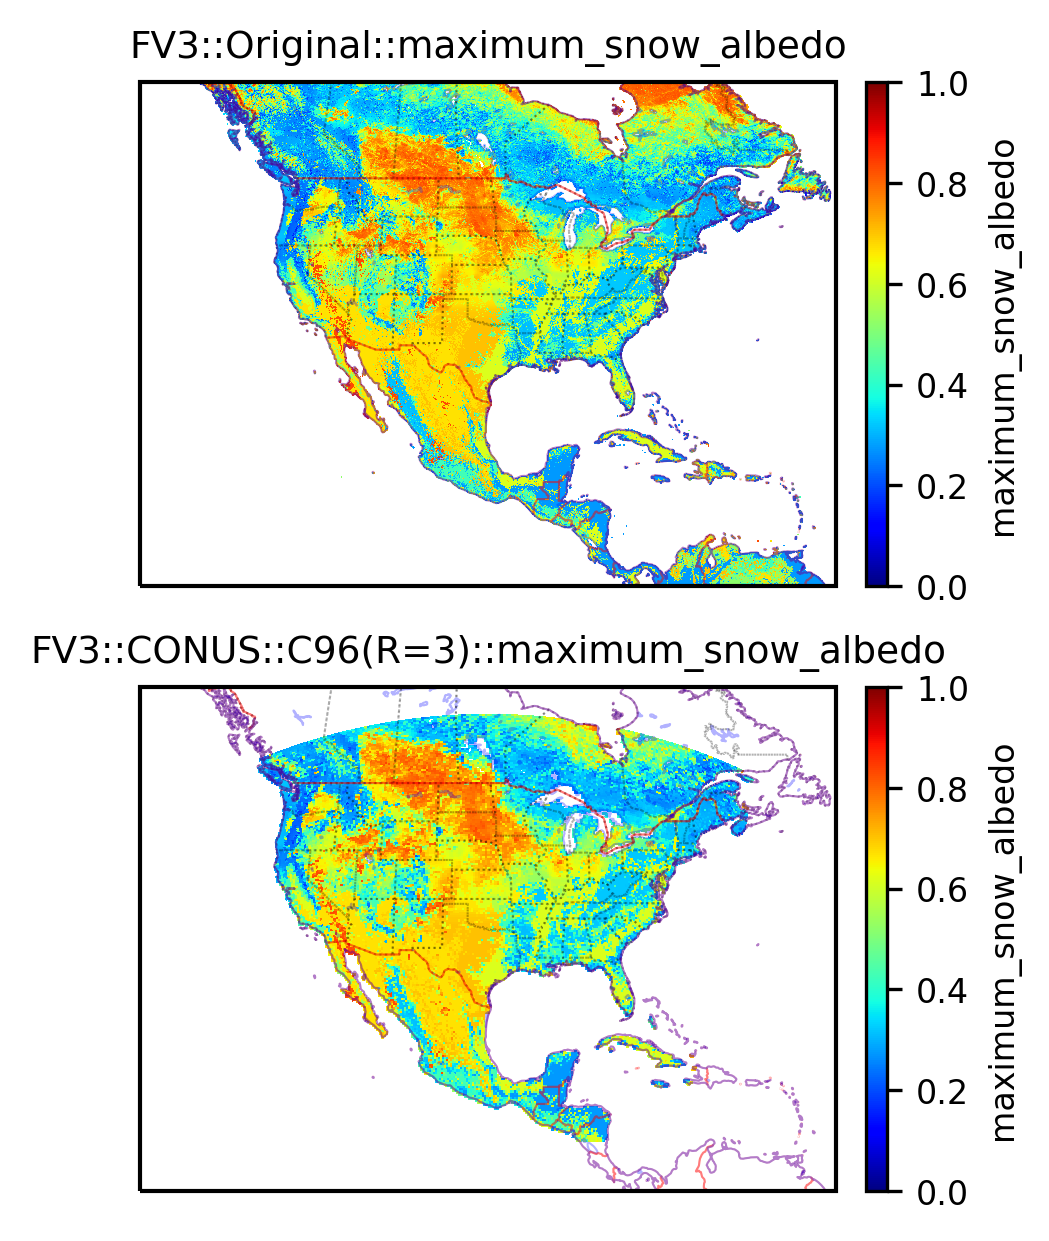
\includegraphics[width=0.46\linewidth]{fv3_static_CONUS_C96_maximum_snow_albedo.png}
  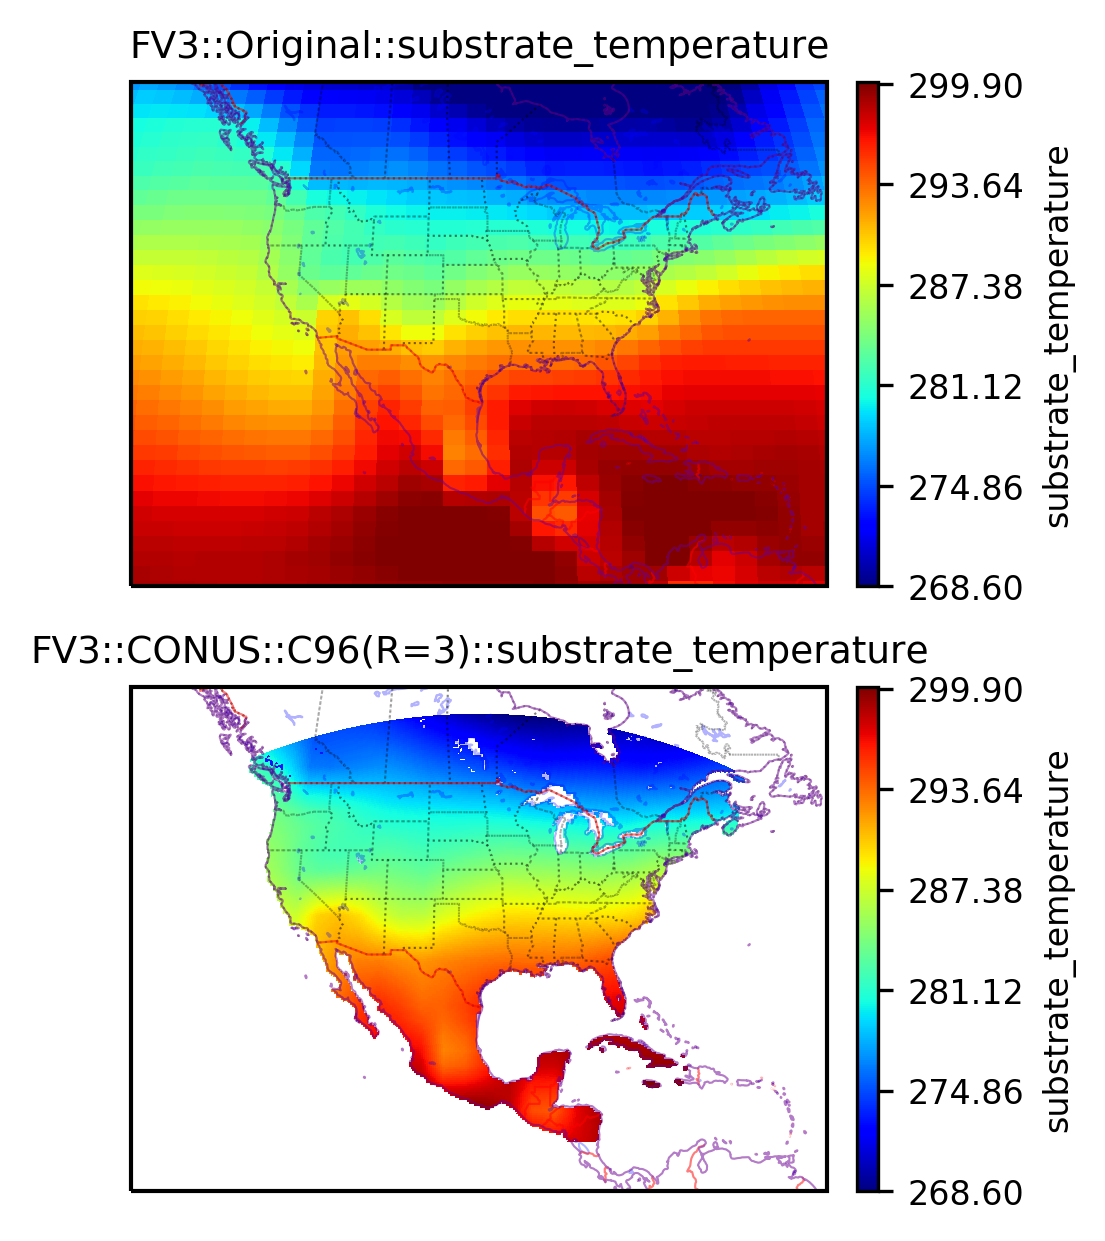
\includegraphics[width=0.48\linewidth]{fv3_static_CONUS_C96_substrate_temperature.png}
  \caption{Maximum snow albedo, and Substrate temperature}
  \label{fig:py_stt_maxsnow}
\end{figure}


\end{enumerate}




%-------------------------------------------
\subsection{Static Fields: Global (`fix\_am')}

The python script `plot\_fv3lam\_fixam.py' creates figures for global static fields (input files, format: GRB) in the directory of `fix\_am'. The required files can be found in the namelist as described in Table \ref{table:fv3_input_nml_namsfc}.

\begin{enumerate}
\item Input files
\begin{itemize}
\item global\_glacier.2x2.grb
\item global\_maxice.2x2.grb
\item global\_snoclim.1.875.grb
\item global\_soilmgldas.t1534.3072.1536.grb
\item CFSR.SEAICE.1982.2012.monthly.clim.grb
\item RTGSST.1982.2012.monthly.clim.grb
\end{itemize}
\item Output files
\begin{itemize}
\item fv3lam\_fixam\_\{variable\}.png
\item fv3lam\_fixam\_\{variable\}\_m\{month\}.png
\item fv3lam\_fixam\_\{variable\}\_m\{month\}\_L\{level\}.png
\end{itemize}
\item Run on HPC

\begin{itemize}
\item On Hera:
\lstset{language=bash}   
\begin{lstlisting}[frame=trBL]
# Check Input and Output paths and names
vim plot_fv3lam_fixam.py
# Submit interactive job for a long run-time (<30min)
salloc -q debug -t 0:30:00 --nodes=1 -A fv3-cam
# Run python script
python3 plot_fv3lam_fixam.py
\end{lstlisting}

\item On Orion:
\lstset{language=bash}   
\begin{lstlisting}[frame=trBL]
# Check Input and Output paths and names
vim plot_fv3lam_fixam.py
# Interactive mode on HPC
salloc --ntasks=1 --time=00:30:00 
# Run the script
python3 plot_fv3lam_fixam.py
\end{lstlisting}

\end{itemize}

{
\fontsize{10}{12}\selectfont
\begin{longtable}{p{0.15\linewidth} | p{0.72\linewidth} }
\hline
\hline
Name & Description \\
\hline
 machine & HPC machine for plotting \\
 out\_fig\_dir & Path to the directory where output files are created \\
 dnm\_data & Path to the directory where the input NetCDF files are located   \\
 vars\_fixam & Specific field name of the input files \\
 out\_title\_base & Basic form of the title in the figures \\
 out\_fname\_base & Basic form of the output file name for the fields \\
 back\_res & Resolution of the background plot \\
\hline
\caption{Namelist in the script for plotting global static fields.}
\label{table:fv3_var_fixam}
\end{longtable}
}

\item Output: sea Surface Temperature, and soilmgldas (March, L10)
\begin{figure}[ht!]
  \centering
  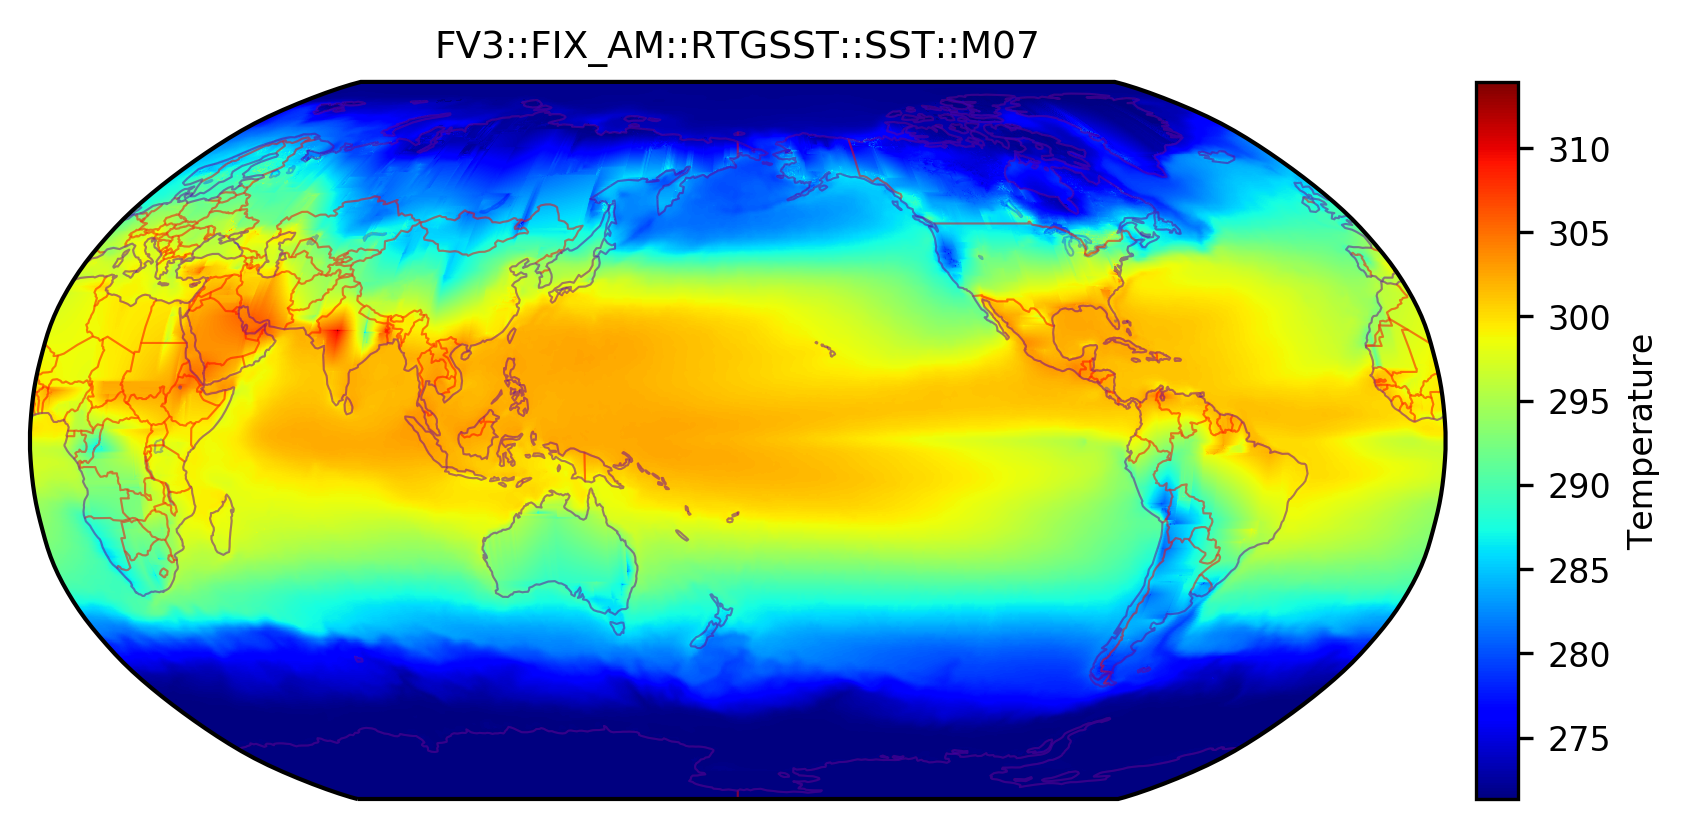
\includegraphics[width=0.6\linewidth]{fv3_fixam_RTGSST_m07.png}
  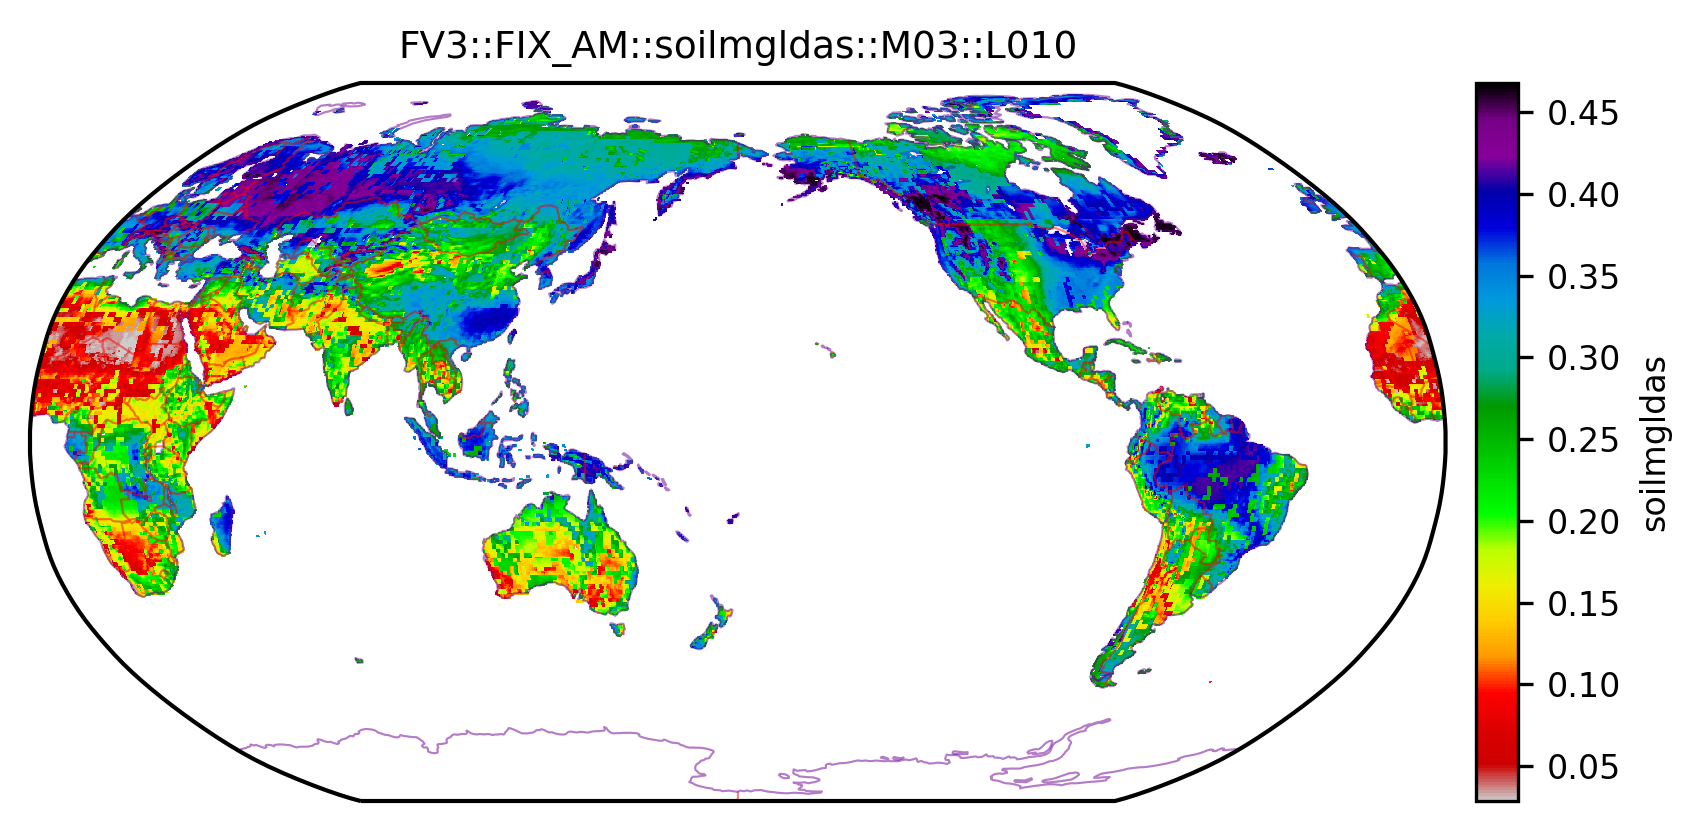
\includegraphics[width=0.6\linewidth]{fv3_fixam_soilmgldas_m03_L010.png}
  \caption{Sea surface temperature, and soilmgldas}
  \label{fig:py_fxam_sst}
\end{figure}

\end{enumerate}



%-------------------------------------------
\subsection{Time-dependent IC/LBC Fields}

The python script `plot\_fv3lam\_icbc.py' creates figures for time-dependent initial (IC) and lateral boundary (LBC) fields on the halo and blending layers along the boundary of a regional domain as well as the original data of the fields for comparison. Since `halo=4', `$0\le$n\_blend$\le10$', and the number of grid points along the axis is more than 190, the IC/LBC fields in the files are too narrow and long to plot in the regular coordinate system. Therefore, the target areas in this script are four corners of the domain. Since {\it FV3} uses the Arakawa C and D grid systems, velocity components are evaluated at the centers of top, bottom, left, and right grid faces. Therefore, some of top, bottom, left, and right boundaries have one more layer (row/column) than other fields depending on which component is evaluated. The axes of top, bottom, left, and right are contracted to the middle of the axes to secure reasonable spaces for comparison between cells near the corners. However, this approach makes us look some discontinuous points. To verify the boundary fields, this script creates another file for the original GFS data. Since this GFS file contains the initial condition at t=000, it should be compared to the data of `gfs\_bndy.tile7.000.nc'. The figure shows two different coordinate systems with the same data: (1) general equi-distant spacing, and (2) contracted spacing to the middle, which is the same as the boundary plot.

\begin{enumerate}
\item Input files
\begin{itemize}
\item gfs\_bndy.tile7.[XXX].nc     (for boundary plot)
\item gfs\_data.tile7.nc     (for initial GFS data plot in the main domain)
\end{itemize}
\item Output files
\begin{itemize}
\item fv3lam\_icbc\_\{Variable\}\_L\{layer number\}\_t\{time\}\_B\{n\_blend\}.png (boundary)
\item fv3lam\_icbc\_\{Variable\}\_L\{layer number\}\_gfs.png (initial GFS data)
\end{itemize}
\item Run on HPC

\lstset{language=bash}   
\begin{lstlisting}[frame=trBL]
# Check Input and Output paths and names
vim plot_fv3lam_icbc.py
# Run the script
python3 plot_fv3lam_icbc.py
\end{lstlisting}

\end{enumerate}

{
\fontsize{10}{12}\selectfont
\begin{longtable}{p{0.17\linewidth} | p{0.7\linewidth} }
\hline
\hline
Name & Description \\
\hline
 machine & HPC machine for plotting \\
 out\_fig\_dir & Path to the directory where output files are created \\
 dnm\_data & Path to the directory where the input NetCDF files are located   \\
 fnm\_in\_bndr\_base & Basic form of the input NetCDF files \\
 bndr\_step & Time steps in the file names \\
 vars\_bc & Variables for plotting \\
 ilvl & Specific number of the vertical level (layer number) for 3-D variables \\
 out\_title\_base & Basic form of the title in the figure \\
 out\_fname\_base & Basic form of the output file name \\
 n\_halo & Number of additional boundary arrays (halo), typically halo=4 \\
 n\_blend & Number of blending layers \\
\hline
\caption{Namelist in the script for plotting IC/LBC fields.}
\label{table:fv3_var_icbc}
\end{longtable}
}

{\bf Notes)}
\begin{itemize}
\item The namelist of the tracers can be found in Table \ref{table:fv3_fld_tracers}.
\item In the figures, the dashed lines in white represent the boundary of the regional domain.
\item Total number of layers = n\_halo + n\_blend.
\end{itemize}


\begin{figure}[ht!]
  \centering
  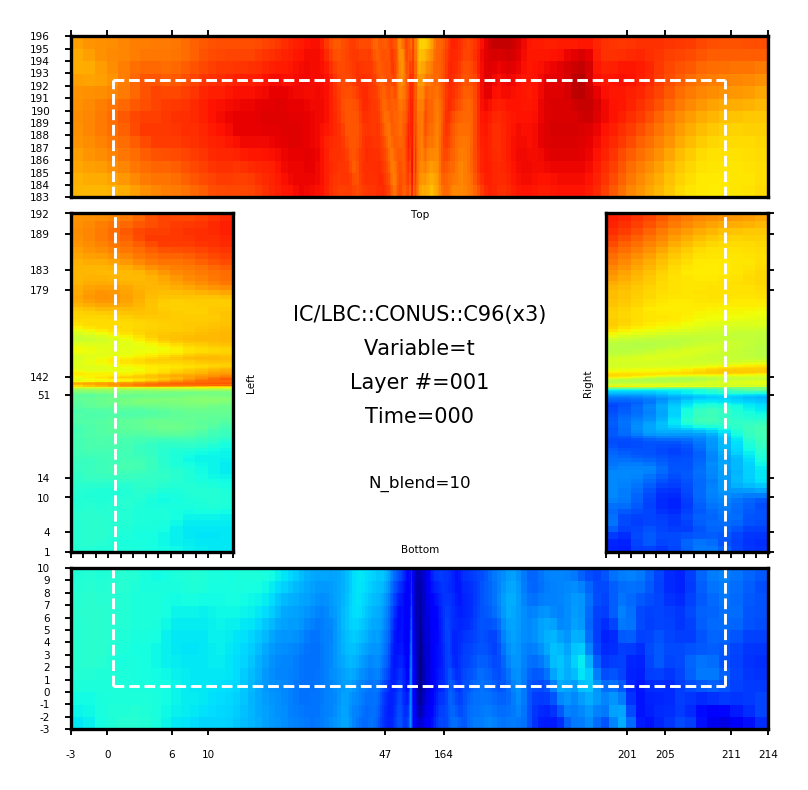
\includegraphics[width=0.65\linewidth]{fv3_icbc_CONUS_C96_t_L001_t000_B10.png}
  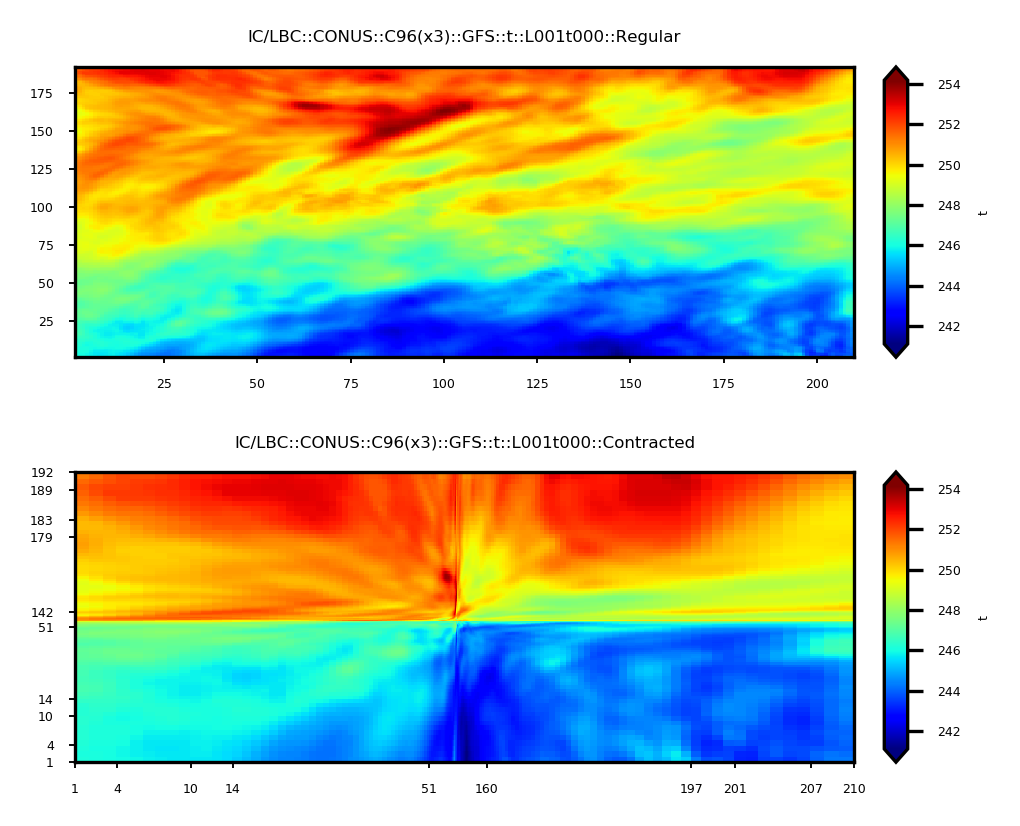
\includegraphics[width=0.7\linewidth]{fv3_icbc_CONUS_C96_t_L001_gfs.png}  
  \caption{Temperature (t) along the boundary at the first layer (initial boundary condition, time=000, layer number=1) and GFS data inside the domain}
  \label{fig:py_icbc_vs}
\end{figure}

\clearpage


%-------------------------------------------
\subsection{Initial Surface Climatology Fields}

This script creates a figure to illustrate surface climatology fields in the input `fix' files.

\begin{enumerate}
\item Input files
\begin{itemize}
\item sfc\_data.nc
\item oro\_data.nc 
\end{itemize}
\item Output files
\begin{itemize}
\item fv3lam\_isfc\_\{domain\}\_C\{res\}\_\{Variable\}.png
\end{itemize}
\item Run on HPC

\lstset{language=bash}   
\begin{lstlisting}[frame=trBL]
# Check Input and Output paths and names
vim plot_fv3lam_isfc.py
# Run the script
python3 plot_fv3sar_isfc.py
\end{lstlisting}

{
\fontsize{10}{12}\selectfont
\begin{longtable}{p{0.17\linewidth} | p{0.7\linewidth} }
\hline
\hline
Name & Description \\
\hline
 machine & HPC machine for plotting \\
 out\_fig\_dir & Path to the directory where output files are created \\ 
 dnm\_data & Path to the directory where the input NetCDF files are located   \\
 oro\_path & Path to the orography file \\
 fnm\_input & Input NetCDF file \\
 fnm\_in\_orog & Input orography file \\
 vars\_isfc & plotting variables in the data file (Table \ref{table:fv3_fld_gfssfc}) \\
 out\_title\_base & Basic form of the title in the figure \\
 out\_fname\_base & Basic form of the output file name \\
 back\_res & Background resolution \\
\hline
\caption{Namelist for plotting initial surface climatology.}
\label{table:fv3_var_isfc}
\end{longtable}
}


\item Output:

\begin{figure}[ht!]
  \centering
  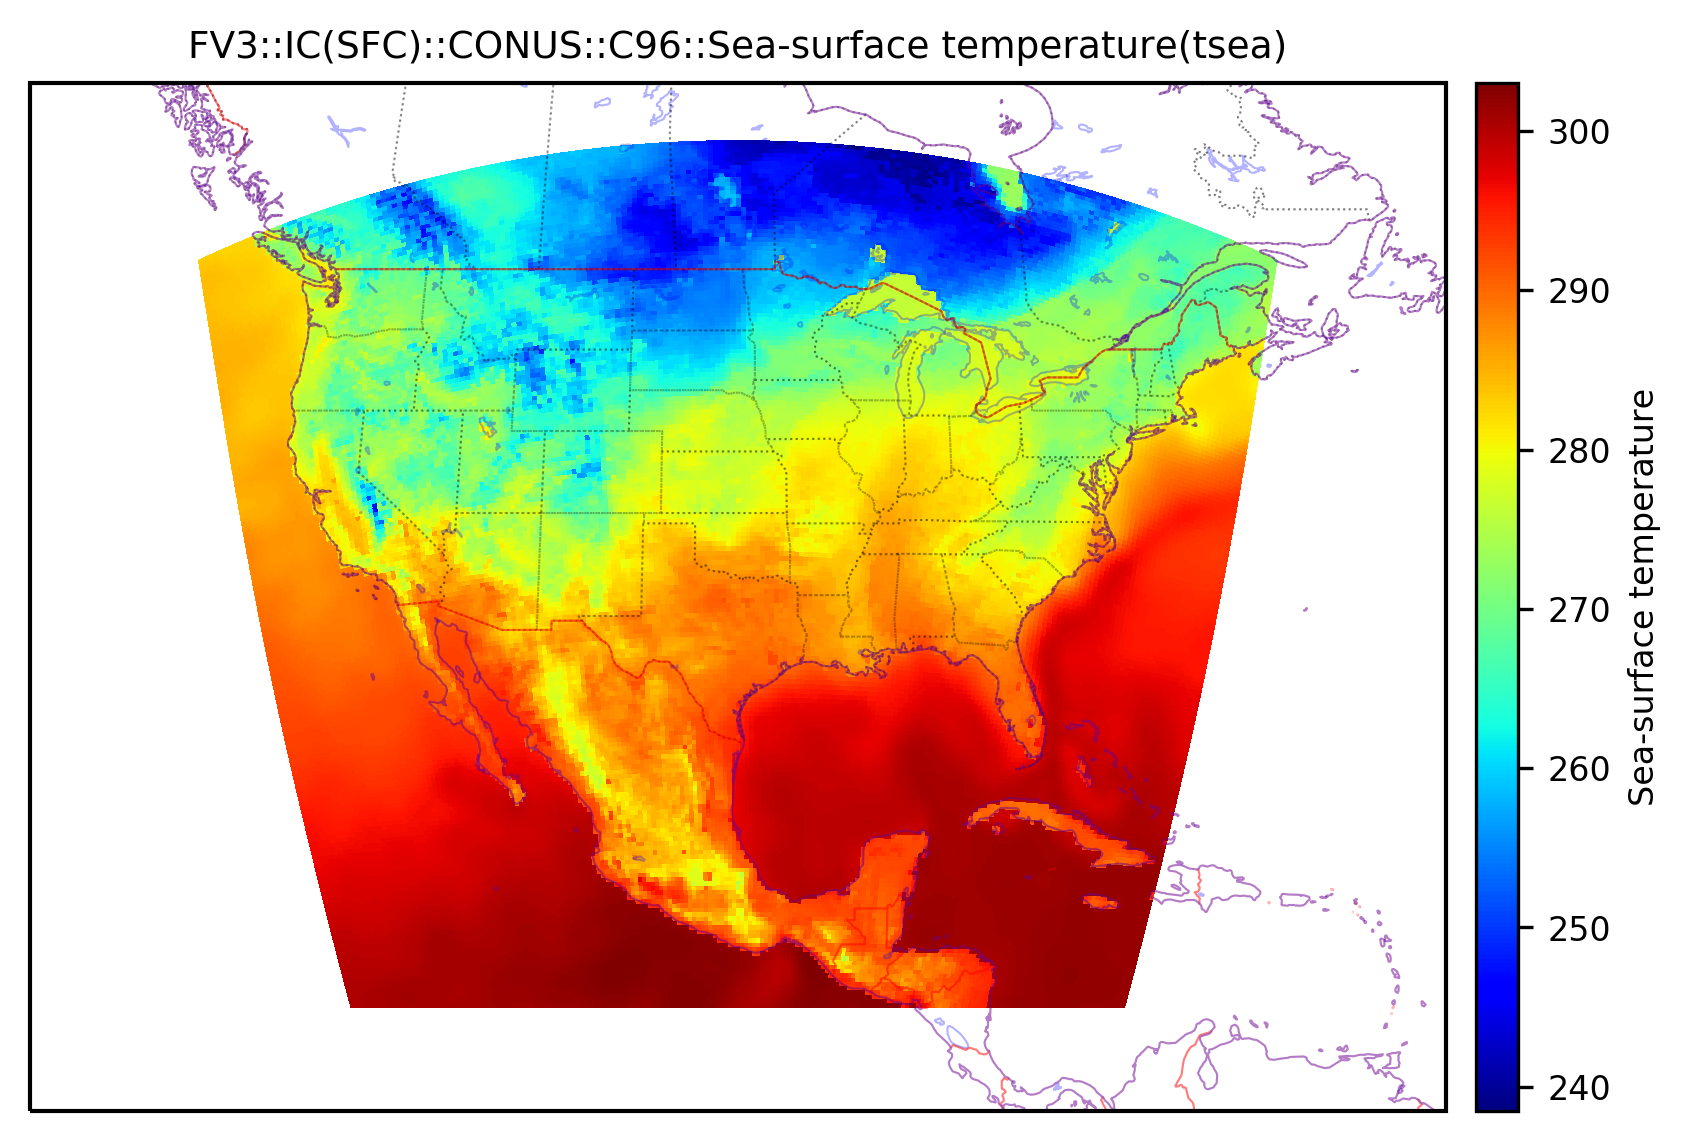
\includegraphics[width=0.48\linewidth]{fv3_isfc_CONUS_C96_tsea.png}
  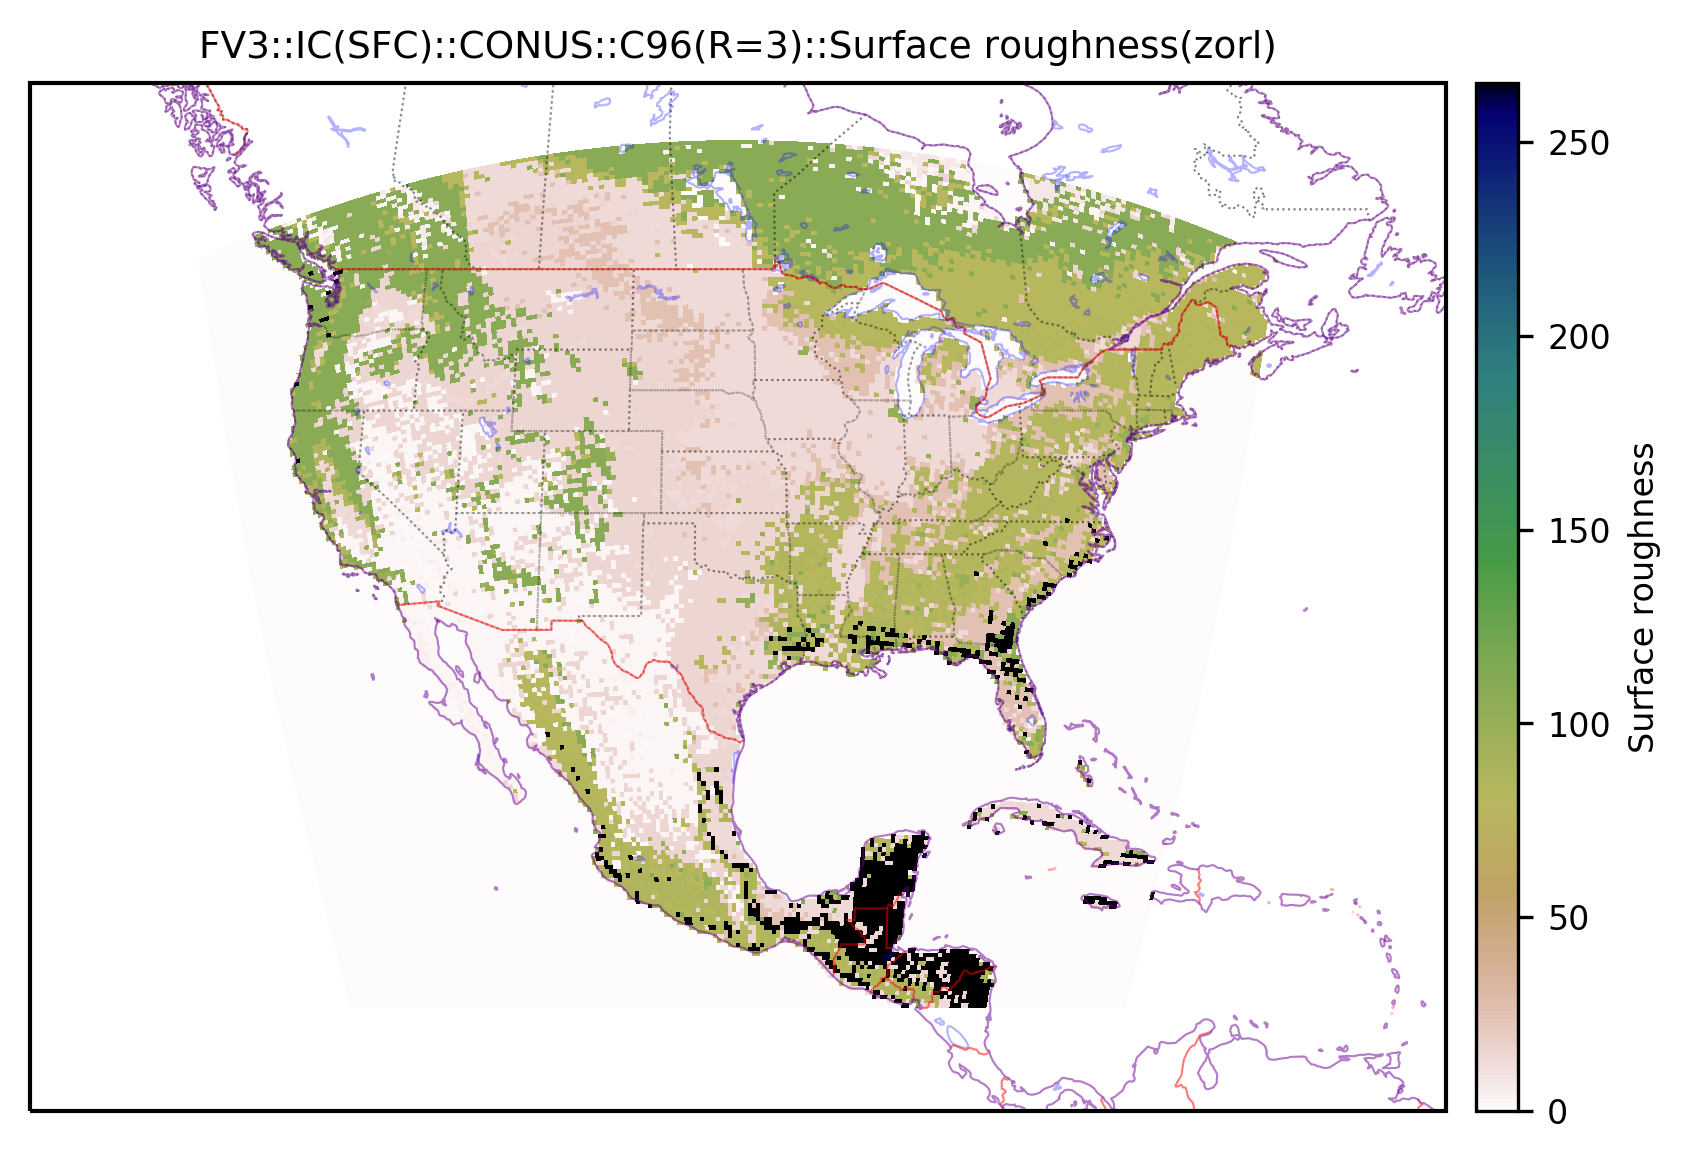
\includegraphics[width=0.48\linewidth]{fv3_isfc_CONUS_C96_zorl.png}  
  \caption{Sea-surface temperature, and roughness}
  \label{fig:py_isfc_zorl}
\end{figure}


\end{enumerate}




%-------------------------------------------
\subsection{Historical CO$_2$ Data}

This script creates figures to illustrate monthly CO$_2$ data in the input `co2historicaldata\_20XX.txt' file.

\begin{enumerate}
\item Input files
\begin{itemize}
\item co2historicaldata\_20XX.txt
\end{itemize}
\item Output files
\begin{itemize}
\item fv3lam\_co2his\_m\{month\}.png
\end{itemize}
\item Run on HPC

\lstset{language=bash}   
\begin{lstlisting}[frame=trBL]
# Check Input and Output paths and names
vim plot_fv3lam_co2his.py
# Run the script
python3 plot_fv3lam_co2his.py
\end{lstlisting}

{
\fontsize{10}{12}\selectfont
\begin{longtable}{ p{0.17\linewidth} | p{0.7\linewidth} }
\hline
\hline
 Name & Description \\
\hline
 machine & HPC machine for plotting \\
 out\_fig\_dir & Path to the directory where output files are created \\
 dnm\_data & Path to the directory where the input file is located   \\
 fnm\_in & Input text file \\
 out\_title\_base & Base of the figure title \\
 out\_fname\_base & Base of the output file name \\
 back\_res & Background resolution \\
\hline
\caption{Namelist in the script for plotting `grid\_spec'.}
\label{table:fv3_var_gridspec}
\end{longtable}
}


\item Output:

\begin{figure}[ht!]
  \centering
  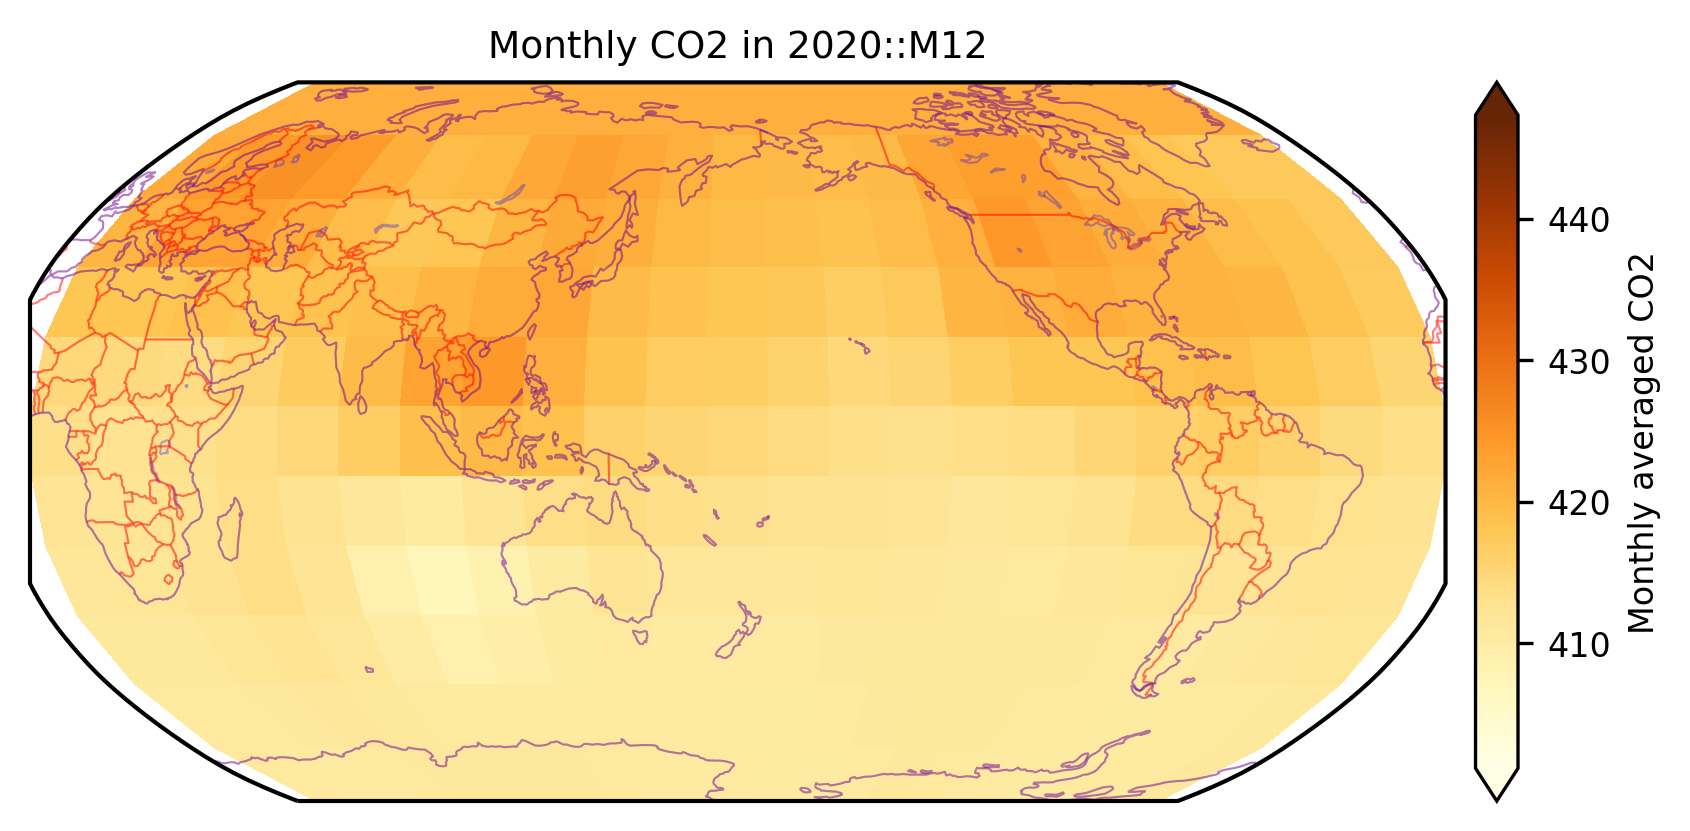
\includegraphics[width=0.5\linewidth]{fv3_co2his_m12.png}
  \caption{Monthly CO$_2$ input data}
  \label{fig:py_fv3_co2his}
\end{figure}

\end{enumerate}



%-------------------------------------------
\subsection{Output: `grid\_spec'}

This script creates a figure to illustrate some grid points in the output `gird\_spec.nc' file.

\begin{enumerate}
\item Input files
\begin{itemize}
\item grid\_spec.nc
\item grid.tile7.halo4.nc
\item oro\_data.tile7.halo4.nc
\end{itemize}
\item Output files
\begin{itemize}
\item fv3lam\_out\_grdspec\_\{domain\}\_C\{res\}.png
\end{itemize}
\item Run on HPC

\lstset{language=bash}   
\begin{lstlisting}[frame=trBL]
# Check Input and Output paths and names
vim plot_fv3lam_gridspec.py
# Run the script
python3 plot_fv3lam_gridspec.py
\end{lstlisting}

{
\fontsize{10}{12}\selectfont
\begin{longtable}{p{0.17\linewidth} | p{0.7\linewidth} }
\hline
\hline
Name & Description \\
\hline
 machine & HPC machine for plotting \\
 out\_fig\_dir & Path to the directory where output files are created \\ 
 dnm\_out & Path to the directory where the input NetCDF files are located   \\
 fnm\_input & Input NetCDF file \\
 n\_gpt & Number of grid points in plot \\
 dnm\_ref & Path to the directory where the grid and orography files are located \\
 fnm\_ref\_grd & Grid file \\
 fnm\_ref\_oro & Orography file \\
 out\_grd\_title\ & Title of the figure \\
 out\_grd\_fname & Output file name \\
 back\_res & Background resolution \\
\hline
\caption{Namelist in the script for plotting `grid\_spec'.}
\label{table:fv3_var_gridspec}
\end{longtable}
}


\item Output:

\begin{figure}[ht!]
  \centering
  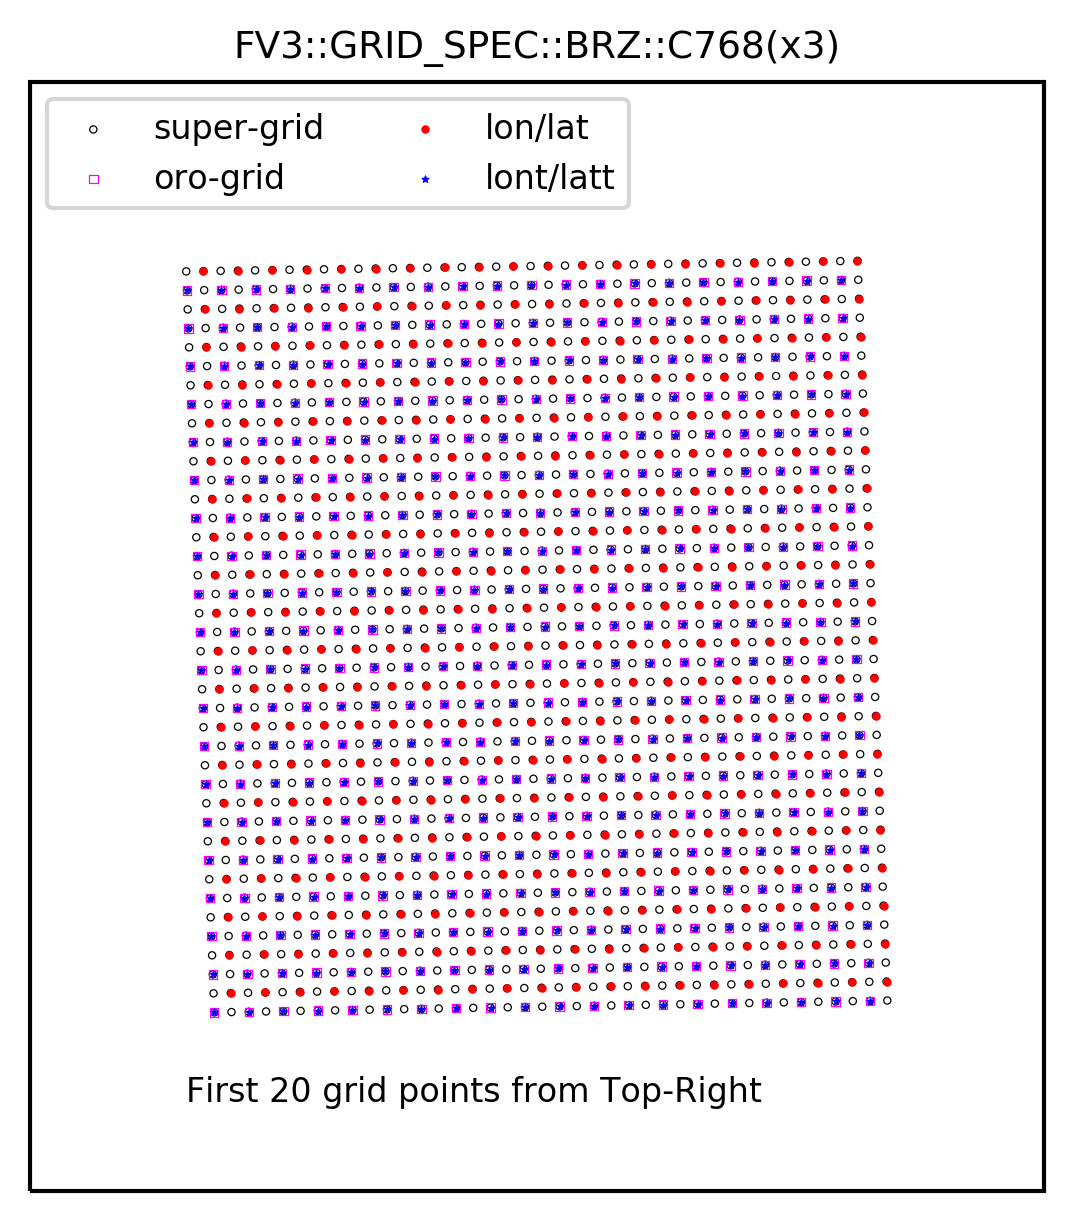
\includegraphics[width=0.45\linewidth]{fv3_out_grdspec_BRZ_C768.png}
  \caption{Output: grid\_spec}
  \label{fig:py_out_gridspec}
\end{figure}

\end{enumerate}



%-------------------------------------------
\subsection{Output: `atmos\_static'}

\begin{enumerate}
\item Input files
\begin{itemize}
\item atmos\_static.nc
\item oro\_data.nc
\end{itemize}
\item Output files
\begin{itemize}
\item fv3lam\_out\_atmfix\_[variable].png
\end{itemize}
\item Run on HPC

\lstset{language=bash}   
\begin{lstlisting}[frame=trBL]
# Check Input and Output paths and names
vim plot_fv3lam_atmfix.py
# Run the script
python3 plot_fv3lam_atmfix.py
\end{lstlisting}

{
\fontsize{10}{12}\selectfont
\begin{longtable}{p{0.17\linewidth} | p{0.7\linewidth} }
\hline
\hline
 Name & Description \\
\hline
 machine & HPC machine for plotting \\
 data\_dir & Path to the Natural Earth data for background \\
 out\_fig\_dir & Path to the directory where output files are created \\
 mfdf\_kwargs & mfdataset argument \\
 dnm\_out & Path to the directory where the input NetCDF files are located   \\
 fnm\_input & Input NetCDF file \\
 dnm\_ref & Path to the directory where the grid and orography files are located \\
 fnm\_ref\_oro & Orography file \\
 vars\_atm & Variables in the input file, which can be found in Table \ref{table:fv3_out_grid_spec}\\
 out\_title\_base & Title of the figure \\
 out\_fname\_base & Output file name \\
 back\_res & Background resolution \\
\hline
\caption{Namelist in the script for plotting `atmos\_static'.}
\label{table:fv3_var_atmosstatic}
\end{longtable}
}


\item Output:

\begin{enumerate}
\item One-dimensional data:
\begin{figure}[ht!]
  \centering
  \includegraphics[width=0.48\linewidth]{fv3_out_atmfix_BRZ_C768_pk.png}
  \includegraphics[width=0.47\linewidth]{fv3_out_atmfix_BRZ_C768_bk.png}  
  \caption{Output: atmos\_static (`pk' and `bk')}
  \label{fig:py_out_atmfix_1d}
\end{figure}

\item Two-dimensional data:
\begin{figure}[ht!]
  \centering
  \includegraphics[width=0.6\linewidth]{fv3_out_atmfix_BRZ_C768_zsurf.png}  
  \caption{Output: atmos\_static (`zsurf')}
  \label{fig:py_out_atmfix_2d}
\end{figure}
\end{enumerate}

\end{enumerate}




%-------------------------------------------
\subsection{Output: `fv3\_history2d' - Boundary}
\label{subsec:python_his2d_bndr}

This script creates figures to illustrate boundary regions of the output `fv3\_history2d.nc' file as well as the entire domain.

\begin{enumerate}
\item Input files
\begin{itemize}
\item fv3\_history2d.nc
\end{itemize}
\item Output files
\begin{itemize}
\item fv3lam\_out\_his2d\_[variable]\_domain.png
\item fv3lam\_out\_his2d\_[variable]\_bndr.png
\end{itemize}
\item Run on HPC

\lstset{language=bash}   
\begin{lstlisting}[frame=trBL]
# Check Input and Output paths and names
vim plot_fv3lam_his2d_bndr.py
# Run the script
python3 plot_fv3lam_his2d_bndr.py
\end{lstlisting}

{
\fontsize{10}{12}\selectfont
\begin{longtable}{ p{0.17\linewidth} | p{0.7\linewidth} }
\hline
\hline
Name & Description \\
\hline
 machine & HPC machine for plotting \\
 dnm\_in & Path to the directory where the input NetCDF files are located   \\
 fnm\_input & Input file name \\
 vars\_his & Variable of input file to be plotted \\
 prt\_tlvl & Time level of plotting \\
 len\_bndr & Length of boundary in plotting (unit: grid points) \\
 dtick\_s & Tick interval for short sides of boundary regions \\
 dtick\_l & Tick interval for long sides of boundary regions \\
 out\_fig\_dir & Path to the directory where output files are created \\
 out\_title\_base & Title of the figure \\
 out\_fname\_base & Output file name \\
\hline
\caption{Namelist in the script for plotting `fv3\_his2d\_bndr'.}
\label{table:fv3_var_dyn}
\end{longtable}
}

\item Output:
\begin{figure}[ht!]
  \centering
  \includegraphics[width=0.6\linewidth]{fv3_out_his2d_HRRR_esg_C768_tmpsfc_domain.png}  
  \caption{Output: fv3\_history2d\_domain}
  \label{fig:py_out_his2d_domain}
\end{figure}

\begin{figure}[ht!]
  \centering
  \includegraphics[width=0.6\linewidth]{fv3_out_his2d_HRRR_esg_C768_tmpsfc_bndr.png}
  \caption{Output: fv3\_history2d\_bndr}
  \label{fig:py_out_his2d_bndr}
\end{figure}

\end{enumerate}




%-------------------------------------------
\subsection{Output: `dynf'}
\label{subsec:python_dynf}

\begin{enumerate}
\item Input files
\begin{itemize}
\item dynfXXX.nc
\end{itemize}
\item Output files
\begin{itemize}
\item fv3\_out\_dyn\_[variable].png
\end{itemize}
\item Run on HPC

\lstset{language=bash}   
\begin{lstlisting}[frame=trBL]
# Check Input and Output paths and names
vim plot_fv3lam_dynf.py
# Run the script
python3 plot_fv3lam_dynf.py
\end{lstlisting}

{
\fontsize{10}{12}\selectfont
\begin{longtable}{p{0.17\linewidth} | p{0.7\linewidth} }
\hline
\hline
 Name & Description \\
\hline
 machine & HPC machine for plotting \\
 data\_dir & Path to the Natural Earth data for background \\
 out\_fig\_dir & Path to the directory where output files are created \\
 mfdf\_kwargs & mfdataset argument \\
 dnm\_out & Path to the directory where the input NetCDF files are located   \\
 fnm\_hr & Input file number \\
 vars\_dyn & Variables in the input file, which can be found in Section \ref{subsec:diag_table}\\
 lvl & Vertical layer number (only for 3-dimensional) \\
 out\_title\_base & Title of the figure \\
 out\_fname\_base & Output file name \\
 back\_res & Background resolution \\
\hline
\caption{Namelist in the script for plotting `dynfXXX'.}
\label{table:fv3_var_dyn}
\end{longtable}
}

{\bf Note)} Since `dynf' and `phyf' are the results of the write component option (`quilting=.true.'), their coordinates (longitude and latitude) would be different from those of input grid and orography, and output `grid\_spec.nc' files.


\item Output:

\begin{figure}[ht!]
  \centering
  \includegraphics[width=0.8\linewidth]{fv3_out_dyn_CONUS_C96_ustm_f001.png}
  \caption{Output: dynfXXX}
  \label{fig:py_out_dyn}
\end{figure}

\end{enumerate}



%-------------------------------------------
\subsection{Output: `phyf'}
\label{subsec:python_phyf}

\begin{enumerate}
\item Input files
\begin{itemize}
\item phyfXXX.nc
\end{itemize}
\item Output files
\begin{itemize}
\item fv3lam\_out\_phy\_[variable].png
\end{itemize}
\item Run on HPC

\lstset{language=bash}   
\begin{lstlisting}[frame=trBL]
# Check Input and Output paths and names
vim plot_fv3lam_phyf.py
# Run the script
python3 plot_fv3lam_phyf.py
\end{lstlisting}

{
\fontsize{10}{12}\selectfont
\begin{longtable}{p{0.17\linewidth} | p{0.7\linewidth} }
\hline
\hline
Name & Description \\
\hline
 machine & HPC machine for plotting \\
 out\_fig\_dir & Path to the directory where output files are created \\
 dnm\_out & Path to the directory where the input NetCDF files are located   \\
 fnm\_hr & Input file number \\
 vars\_phy & Variables in the input file, which can be found in Section \ref{subsec:diag_table}\\
 out\_title\_base & Title of the figure \\
 out\_fname\_base & Output file name \\
 back\_res & Background resolution \\
\hline
\caption{Namelist in the script for plotting `phyfXXX'.}
\label{table:fv3_var_phy}
\end{longtable}
}

\item Output:

\begin{figure}[ht!]
  \centering
  \includegraphics[width=0.8\linewidth]{fv3_out_phy_CONUS_C96_u10max_f001.png}
  \caption{Output: phyfXXX}
  \label{fig:py_out_phy}
\end{figure}

\end{enumerate}



%-------------------------------------------
\subsection{Output: `BGRD3D (natlev.grib2)'}
\label{subsec:python_BGRD3D}

\begin{enumerate}
\item Input files
\begin{itemize}
\item rrfs.tXXz.bgrd3dfXXX.tmXX.grib2 (*.natlev.grib2)
\end{itemize}
\item Output files
\begin{itemize}
\item fv3lam\_out\_bgrd3d\_fXXX\_[variable].png
\end{itemize}
\item Run on HPC

\lstset{language=bash}   
\begin{lstlisting}[frame=trBL]
# Check Input and Output paths and names
vim plot_fv3lam_bgrd3d.py
# Run the script
python3 plot_fv3lam_bgrd3d.py
\end{lstlisting}

{
\fontsize{10}{12}\selectfont
\begin{longtable}{ p{0.17\linewidth} | p{0.7\linewidth} }
\hline
\hline
 Name & Description \\
\hline
 machine & HPC machine for plotting \\
 out\_fig\_dir & Path to the directory where output files are created \\
 dnm\_data & Path to the directory where the input GRIB2 file is located   \\
 fnm\_hr & Input file hour number (`fXXX') \\
 fnm\_in & Input file name \\
 vars\_grb2 & Variables in the input file (Table \ref{table:fv3_grb2_lev_table})\\
 nlvl & Total number of vertical layers in the model \\
 ilvl & Layer number to be plotted \\
 out\_title\_base & Title of the figure \\
 out\_fname\_base & Output file name \\
 back\_res & Background resolution (`10m', `50m', `100m') \\
 back\_img & Background image (`on', `off') \\
\hline
\caption{Namelist in the script for plotting `bgrd3d.grib2'.}
\label{table:fv3_var_lev_grib2}
\end{longtable}
}

\item Output:

\begin{figure}[ht!]
  \centering
  \includegraphics[width=0.8\linewidth]{fv3_out_lev_CONUS_C96_t_hybrid_L001.png}
  \caption{Output: BGRD3D (grib2)}
  \label{fig:py_out_lev}
\end{figure}

\end{enumerate}



%-------------------------------------------
\subsection{Output: `BGDAWP (natprs.grib2)'}
\label{subsec:python_BGDAWP}

\begin{enumerate}
\item Input files
\begin{itemize}
\item rrfs.tXXz.bgdawpfXXX.tmXX.grib2 (*.natprs.grib2)
\end{itemize}
\item Output files
\begin{itemize}
\item fv3lam\_out\_bgdawp\_fXXX\_[variable].png
\end{itemize}
\item Run on HPC

\lstset{language=bash}   
\begin{lstlisting}[frame=trBL]
# Check Input and Output paths and names
vim plot_fv3lam_bgdawp.py
# Run the script
python3 plot_fv3lam_bgdawp.py
\end{lstlisting}

{
\fontsize{10}{12}\selectfont
\begin{longtable}{p{0.17\linewidth} | p{0.7\linewidth} }
\hline
\hline
Name & Description \\
\hline
 machine & HPC machine for plotting \\
 data\_dir & Path to the Natural Earth data for background \\
 out\_fig\_dir & Path to the directory where output files are created \\
 dnm\_out & Path to the directory where the input GRIB2 file is located   \\
 fnm\_hr & Input file hour number (`fXXX') \\
 fnm\_in & Input file name \\
 vars\_grb2 & Variables in the input file (Table \ref{table:fv3_grb2_prs_table})\\ 
 ilvl & Layer number to be plotted \\
 out\_title\_base & Title of the figure \\
 out\_fname\_base & Output file name \\
 back\_res & Background resolution (`10m', `50m', `100m') \\
 back\_img & Background image (`on', `off') \\
\hline
\caption{Namelist in the script for plotting `bgdawp.grib2'.}
\label{table:fv3_var_prs_grib2}
\end{longtable}
}

\item Output:

\begin{figure}[ht!]
  \centering
  \includegraphics[width=0.8\linewidth]{fv3_out_prs_CONUS_C96_tp_surface_L001.png}
  \caption{Output: BGRAWP (grib2)}
  \label{fig:py_out_prs}
\end{figure}

\end{enumerate}




%-------------------------------------------
\subsection{Output: Comparison of Two NetCDF (GRIB2) Files}

This script creates a figure to illustrate a comparison between two NetCDF or GRIB2 files on the same grid.

\begin{enumerate}
\item Input files
\begin{itemize}
\item Two NetCDF or GRIB2 files on the same grid.
\end{itemize}
\item Output files
\begin{itemize}
\item fv3lam\_comp\_[variable].png
\end{itemize}
\item Run on HPC

\lstset{language=bash}   
\begin{lstlisting}[frame=trBL]
# Check Input and Output paths and names
vim plot_fv3lam_comp2f.py
# Run the script
python3 plot_fv3lam_comp2f.py
\end{lstlisting}


{
\fontsize{10}{12}\selectfont
\begin{longtable}{p{0.17\linewidth} | p{0.7\linewidth} }
\hline
\hline
Name & Description \\
\hline
 machine & HPC machine for plotting \\
 out\_fig\_dir & Path to the directory where output files are created \\
 dnm\_in1 & Path to the directory where the first input file is located   \\
 dnm\_in2 & Path to the directory where the second input file is located   \\
 fnm\_in1 & Name of the first Input file  \\
 fnm\_in2 & Name of the second Input file  \\
 vars\_phy & Variables in the input file \\
 grb\_name &  Name of the variable in GRIB2 (only for GRIB2) \\
 grb\_typlvl & Type of level of the variable in GRIB2 (only for GRIB2) \\
 ilvl & Layer number to be plotted (only for 3-dimensional) \\
 cmp\_lbl & Additional text for comparison in title and label \\
 out\_title\_base & Title of the figure \\
 out\_fname\_base & Output file name \\
 back\_res & Background resolution \\
\hline
\caption{Namelist in the script for plotting comparison.}
\label{table:fv3_var_plot_comp}
\end{longtable}
}

\item Output:

\begin{figure}[ht!]
  \centering
  \includegraphics[width=0.8\linewidth]{fv3_out_comp_CONUS_C96_10u.png}
  \caption{Output: comparison}
  \label{fig:py_out_comp}
\end{figure}

\end{enumerate}




%-------------------------------------------
\subsection{MRMS: Composite Reflectivity Radar Data}
\label{subsec:python_mrms}

\begin{enumerate}
\item Input files
\begin{itemize}
\item QCComposite\_00.50\_[date]\_[time]\_new.grib2 (Composite reflectivity)
\item ref3D\_[date]\_[time]\_new.grib2 (26 layer reflectivity)
\end{itemize}

{\bf Notes)} 
\begin{itemize}
\item The MRMS radar data can be obtained from HPSS as shown in Section \ref{sec:data_from_hpss}.
\item The original GRIB2 file should be converted to complex packing by {\it wgrib2} to avoid an API error using {\it Python}.
\end{itemize}

\item Output files
\begin{itemize}
\item fv3lam\_mrms\_comRefl\_[date]\_[time].png (Composite reflectivity)
\item fv3lam\_mrms\_xzRefl\_[date]\_[time].png (Cross-sectional reflectivity)
\item fv3lam\_mrms\_3dRefl\_[date]\_[time].png (3-D reflectivity)
\end{itemize}
\item Run on HPC

\lstset{language=bash}   
\begin{lstlisting}[frame=trBL]
# Check Input and Output paths and names
vim plot_fv3lam_mrms.py
# Run the script
python3 plot_fv3lam_mrms.py
\end{lstlisting}


{
\fontsize{10}{12}\selectfont
\begin{longtable}{p{0.17\linewidth} | p{0.7\linewidth} }
\hline
\hline
Name & Description \\
\hline
 machine & HPC machine for plotting (`hera' ) \\
 out\_fig\_dir & Path to the directory where output files are created \\
 path\_NE & Path to the Natural Earth data \\
 s\_date & Date of the input data (YYYYMMDD) \\
 s\_time & Time of the input data (HHmm) \\
 dnm\_data & Path to the directory where the input GRIB2 file is located   \\
 fnm\_in\_com & Input file name of composite reflectivity \\
 fnm\_in\_3d & Input file name of 3-D reflectivity \\
 plt\_com & Flag for plotting composite reflectivity (`yes' or `no') \\
 plt\_crx & Flag for plotting cross-sectional reflectivity (`yes' or `no') \\
 crx\_lon / crx\_lat & Longitude/latitude of the target point located at the center of the cross sections (in degrees) \\ 
 crx\_dist & Distance from the target point for the limits of the cross sections (in degrees) \\
 plt\_3d & Flag for plotting 3-dimensional reflectivity (`yes' or `no') \\
 out\_title\_com & Title of the output figure of the composite reflectivity  \\
 out\_fname\_com & Output file name of the composite reflectivity \\
 out\_fname\_crx & Output file name of the cross-sectional reflectivity \\
 out\_fname\_3d & Output file name of the 3-dimensional reflectivity \\
 back\_res & Background resolution (`10m', `50m', `100m') \\
 back\_img & Background image (`on', `off') \\
\hline
\caption{Namelist in the script for plotting `mrms\_rada\_reflectivity.grib2'.}
\label{table:fv3_var_mrms_grib2}
\end{longtable}
}

\item Output:

\begin{figure}[ht!]
  \centering
  \includegraphics[width=\linewidth]{fv3_mrms_comRefl_HRRR_20200618_0600.png}
  \caption{MRMS radar: composite reflectivity}
  \label{fig:py_mrms_composite}
\end{figure}

\clearpage

\begin{figure}[H]
  \centering
  \includegraphics[width=0.8\linewidth]{fv3_mrms_xzRefl_HRRR_20200618_0600.png}
  \caption{MRMS radar: cross-sectional reflectivity}
  \label{fig:py_mrms_xsecton}
\end{figure}

\begin{figure}[ht!]
  \centering
  \includegraphics[width=\linewidth]{fv3_mrms_3dRefl_HRRR_20200618_0600.png}
  \caption{MRMS radar: 3-dimensional reflectivity}
  \label{fig:py_mrms_3d}
\end{figure}


\end{enumerate}



%-------------------------------------------
\subsection{Animation: Hourly Comparison of Composite Reflectivity}
\label{subsec:python_ani_refl}

\begin{enumerate}
\item Input files
\begin{itemize}
\item QCComposite\_00.50\_[date]\_[time]\_new.grib2 (radar data files)
\item rrfs.tXXz.bgdawpf0XX.tmXX.grib2 (FV3-LAM result files)
\end{itemize}

{\bf Notes)} 
\begin{itemize}
\item The MRMS radar data can be obtained from HPSS as shown in Section \ref{sec:data_from_hpss}.
\item The original GRIB2 file should be converted to complex packing by {\it wgrib2} to avoid an API error using {\it Python}.
\end{itemize}

\item Output files
\begin{itemize}
\item fv3lam\_out\_ani\_refl\_comp\_[date].gif
\end{itemize}

\item Run on HPC
\lstset{language=bash}   
\begin{lstlisting}[frame=trBL]
# Check Input and Output paths and names
vim plot_fv3lam_ani_comref.py
# Run the script
python3 plot_fv3lam_ani_comref.py
\end{lstlisting}


{
\fontsize{10}{12}\selectfont
\begin{longtable}{p{0.17\linewidth} | p{0.7\linewidth} }
\hline
\hline
Name & Description \\
\hline
 machine & HPC machine for plotting (`hera' ) \\
 out\_fig\_dir & Path to the directory where output files are created \\
 path\_NE & Path to the Natural Earth data \\
 s\_date & Date in the data directory name (YYYYMMDD) \\
 plot\_hrs & Plotting hours for animation \\
 s\_time & Time of the input data (HHmm) \\
 dnm\_data\_mdl & Path to the directory where the output GRIB2 files are located   \\
 dnm\_data\_dat & Path to the directory where the radar data are located   \\
 svar & Output field name \\
 out\_title\_sub1 & Sub-title of the sub-plot 1 for output data \\
 out\_title\_sub2 & Sub-title of the sub-plot 2 for radar data  \\
 back\_res & Background resolution (`10m', `50m', `100m') \\
 back\_img & Background image (`on', `off') \\
\hline
\caption{Namelist in the script for animation comparing output data.}
\label{table:fv3_var_ani_refl}
\end{longtable}
}

\item Output:

\begin{figure}[H]
  \centering
  \includegraphics[width=0.8\linewidth]{fv3_out_ani_refl_comp_HRRR-2.png}
  \caption{Animation: hourly comparison with the MRMS rada data}
  \label{fig:py_ani_comp_refl}
\end{figure}

\end{enumerate}



%-------------------------------------------
\subsection{Time-history of Maximum Temperature}
\label{subsec:python_thist_grib2}

This script is designed to confirm that the simulation results have been exported to the GRIB2 files successfully and the results on several machines are reasonably close to each other by plotting the maximum values of temperatures at 2 and 100 meters from the multiple result GRIB2 files.

\begin{enumerate}
\item Input files
\begin{itemize}
\item rrfs.tXXz.bgdawpf0XX.tmXX.grib2 (FV3-LAM result files)
\end{itemize}

\item Output files
\begin{itemize}
\item fv3lam\_out\_grb2his\_[machine].gif
\end{itemize}

\item Run on HPC
\lstset{language=bash}   
\begin{lstlisting}[frame=trBL]
# Check Input and Output paths and names
vim plot_fv3lam_grb2his.py
# Run the script
python3 plot_fv3lam_grb2his.py
\end{lstlisting}


{
\fontsize{10}{12}\selectfont
\begin{longtable}{p{0.17\linewidth} | p{0.7\linewidth} }
\hline
\hline
Name & Description \\
\hline
 machine & HPC machine for plotting (`hera', `wcoss\_dell', `wcoss\_cray', `orion' ) \\
 out\_fig\_dir & Path to the directory where output files are created \\
 dnm\_data & Path to the directory where the output GRIB2 files are located   \\
 fnm\_hr\_s & Input file hour range: start \\
 fnm\_hr\_e & Input file hour range: end \\
 fnm\_hr\_i & Input file hour range: interval \\ 
 out\_title & Title of the output figure \\
 out\_fname & File name of the output figure  \\
\hline
\caption{Namelist in the script for time-history of output grib2 files.}
\label{table:fv3_var_his_grib2}
\end{longtable}
}

\item Output:

\begin{figure}[ht!]
  \centering
  \includegraphics[width=0.9\linewidth]{fv3lam_out_grb2his_hera.png}
  \caption{Time-history of output GRIB2 files}
  \label{fig:py_out_grb2his}
\end{figure}


\end{enumerate}




%~~~~~~~~~~~~~~~~~~~~~~~~~~~~~~~~~~~~~~~~~~~~~~~~~~~~~~~~~~~~~~~~~~~~~

\appendix





%************************************************************************************************************************************************************
\chapter{Workflow Manager: {\it Rocoto}}        

Ref.) \url{https://github.com/christopherwharrop/rocoto/wiki/documentation}

%=================================================== 
\section{How the {\it Rocoto} Engine Works}
\label{sec:rocoto}

{\it Rocoto}:
\begin{itemize}
\item is a `Ruby' program that interfaces to the underlying batch system.
\item is designed to run weather and climate workflows (not general purpose).
\item does all the book keeping necessary to submit tasks when dependencies are satisfied and tracks the progress of the workflow.
\item automatically resubmit failed tasks up to a maximum number of attempts, and can recover from system outages.
\item has no control over when jobs start to run.
\item runs one instance of the workflow for a set of user-defined `circles'. A `circle' usually corresponds to a model analysis or initialization time.
\item users must define their workflows with the XML language.
\end{itemize}


\begin{enumerate}
\item Executing workflows:
     \begin{itemize}
     \item The `rocotorun' command is used to run a workflow:
\lstset{language=bash}   
\begin{lstlisting}[frame=trBL]
rocotorun -w /path/to/workflow/xml/file -d /path/to/workflow/database/file
\end{lstlisting}
     where
        \begin{itemize}
     	\item The `-w' flag specifies the name of the workflow definition file. This must be an XML file.
     	\item The `-d' flag specifies the name of the database file that is to be used to store the state of the workflow. The database file is a binary file created and used only by {\it Rocoto} and need not exit prior to the first time the command is run.
     	\end{itemize}
     \item It is very important to understand that the running process is iterative. Each time the above command is executed, {\it Rocoto} performs the following actions:
    	\begin{enumerate}
	\item Read the last known state of the workflow from the database file specified by the `-d' flag.
	\item Query the batch system to acquire the current state of the workflow.
	\item Take actions based on new state information (resubmit crushed jobs or submit next jobs)
	\item Save the current state of the workflow to the file specified by the `-d' flag
	\item Quit 
	\end{enumerate} 
     
     \end{itemize}
     
\item Checking the status of workflows
	\begin{itemize}
	\item `rocotostat': query the status of a set of cycles and tasks.
\lstset{language=bash}   
\begin{lstlisting}[frame=trBL]
rocotostat -w /path/to/workflow/xml/file -d /path/to/workflow/database/file [-c YYYYMMDDHHMM, [YYYYMMDDHHMM, ...]] [-t taskname, [taskname, ...]] [-s] [-T]
\end{lstlisting}
 		\begin{itemize}
		\item The `-c' option allows you to select specific cycles to query.
		\item The `-t' option allows you to select specify tasks.
		\item The `-T' option sorts the output by taskname rather than by cycle.
		\item The `-s' option will provide a summary report of the status of the cycles themselves rather than information about the tasks.
		\end{itemize}

	\item `rocotocheck': query detailed information about a specific task for a specific cycle.
\lstset{language=bash}   
\begin{lstlisting}[frame=trBL]
rocotockeck -w /path/to/workflow/xml/file -d /path/to/workflow/database/file -c YYYYMMDDHHMM -t taskname
\end{lstlisting}
	\end{itemize}

\item Forcing tasks to run
	\begin{itemize}
	\item `rocotoboot': force a task to be submitted, regardless of whether or not dependencies are satisfied or throttling violations would occur.	
\lstset{language=bash}   
\begin{lstlisting}[frame=trBL]
rocotoboot -w /path/to/workflow/xml/file -d /path/to/workflow/database/file -c YYYYMMDDHHMM -t taskname
\end{lstlisting}
	\end{itemize}

\item Rerunning several tasks in the workflow
	\begin{itemize}
	\item `rocotoewind': undo the effect of having run some jobs, and mark those jobs as not having run.
\lstset{language=bash}   
\begin{lstlisting}[frame=trBL]
rocotoewind -w /path/to/workflow/xml/file -d /path/to/workflow/database/file -c YYYYMMDDHHMM -t taskname
\end{lstlisting}
	\end{itemize}

\end{enumerate}



%=================================================== 
\section{{\it Rocoto} XML Language}
\label{sec:rocotoXML}

\begin{enumerate}
\item XML Header

Every XML file must have this text at the top:
\lstset{language=XML}   
\begin{lstlisting}[frame=trBL]
<?xml version="1.0"?>
<!DOCTYPE workflow
[
]>
\end{lstlisting}


\item ENTITY

An `ENTITY' represents a value that is used in lots of places in the XML.
\lstset{language=XML}   
\begin{lstlisting}[frame=trBL]
<!ENTITY CYCLE_THROTTLE "4">
<!ENTITY GTYPE "@[GTYPE:-regional]">
\end{lstlisting}

The `ENTITY' is referenced by the systex, `\&{\it \{ENTITY\_NAME\}};'.
\lstset{language=XML}   
\begin{lstlisting}[frame=trBL]
<!ENTITY HOME_DIR = "chan-hoo.jeon/fv3sar/">
<!ENTITY LOG = "$HOME_DIR;/log">
\end{lstlisting}


\item Tag: <workflow>

This is the main tag for defining workflows. Everything except for the header and ENTITY definitions must be contained within the <workflow> tags.
\lstset{language=XML}   
\begin{lstlisting}[frame=trBL]
<workflow realtime="F" scheduler="moabtorque" cyclelifespan="0:01:00:00" cyclethrottle="5" taskthrottle="5">

# Everything else goes in here

</workflow>
\end{lstlisting}

\begin{enumerate}
\item {\makebox[2.2cm]{{\bf realtime} \hfill}: define whether or not the workflow is to be run in realtime (``T'' or ``True''), or in retrospective mode (``F'' or ``False''). The difference between realtime and retrospective mode is in how cycles are activated. In realtime mode, cycles are activated based on the current time of day. In retrospective mode, there is no time dependency that must be dhered to. Thus cycles will be activated immediately, in chronological order.}

\item {\makebox[2.2cm]{{\bf scheduler} \hfill}: must be set to one of ``sge'', ``lsf'' (for WCOSS), ``torque'', ``moabtorque'' (for Jet), or ``moab'' (for Gaea). This attribute tells {\it Rocoto} which batch system to use when managing the workflow. It is recommended that the keep time be set to a minimum of 24 hours.}

\item {\makebox[2.2cm]{{\bf cyclelifespan} \hfill}: specifies how long a cycle can be active before it expires in the format of ``DD:HH:MM:SS''. Wall-clock-time requests are automatically capped such that they will not exceed the time when a cycle expires. }

\item {\makebox[2.2cm]{{\bf cyclethrottle} \hfill}: limits how many cycles may be active at one time. Cycles are active if they have not expired and not all tasks for the cycle have completed successfully. }

\item {\makebox[2.2cm]{{\bf corethrottle} \hfill}: limits the total number of cores that may be consumed by jobs submitted to the batch system. Any job that is submitted to the batch system, whether it is running or queued, counts against this total.}

\item {\makebox[2.2cm]{{\bf taskthrottle} \hfill}: limits how many tasks may be active at one time. A task is active if a job has been submitted for it and that job has not finished. Any job that is submitted to the batch system, whether it is running or queued, counts against this total.}

\end{enumerate}


\item Tag: <log>

This defines the path and name of {\it Rocoto} log files. In general, it is best to define the name of the log to be dynamically dependent on the cycle being processed.

\lstset{language=XML}   
\begin{lstlisting}[frame=trBL]
<log><cyclestr>&LOG;/workflow_@Y@m@d@H.log</cyclestr></log>
\end{lstlisting}


\item Tag: <cyclestr>

It is often necessary to refer to the various components of the current cycle time when defining various aspects of the workflow. The <cyclestr> tag uses flags to represent the various time components of the current cycle. These flags will be replaced with the appropriate date/time component of the current cycle being processed. They can be used in any combination to represent any date/time string desired inside a <cyclestr> ... </cyclestr> block.

\begin{itemize}
\item {\bf offset}: represents offset before or after the current cycle. The format of the offset attribute is `dd:hh:mm:ss'. Leading field whose values are 0 do not need to be specified.
\end{itemize}

\lstset{language=XML}   
\begin{lstlisting}[frame=trBL]
<cyclestr offset="1:00:00">@Y@m@d@H.log</cyclestr>
\end{lstlisting}

\begin{table}[ht!]
\centering
\caption{<cyclestr> tags:}
{\begin{tabular}{l | l  }
\hline
\hline
Flag & Time component  \\
\hline
@a & Abbreviated weekday name (e.g. ``Sun'') \\
@A & Full weekday name (e.g. ``Sunday'') \\
@b & Abbreviated month name (e.g. ``Jan'') \\
@B & Full month name (e.g. ``January'')\\
@c & Preferred local date and time representation (e.g. ``Thu Jul 5 11:27:59 2012'') \\
@d & Day of month (01--31) \\
@H & Hour of the day, 24 hour clock (00--24) \\
@I & Hour of the day, 12 hour clock (01--12) \\
@j & Day of the year (001--365) \\
@m & Month of the year (01--12) \\
@M & Minute of the hour (00--59) \\
@p & Meridian indicator (``AM'' or ``PM'')\\
@P & Meridian indicator (``am'' or ``pm'') \\
@s & Number of seconds since January 1, 1970 00:00:00 UTC\\
@S & Second of the minute (00--59) \\
@U & Week number of the current year, starting with the first Sunday as the first day \\
@W & Week number of the current year, starting with the first Monday as the first day \\
@w & Day of week (Sunday is 0, 0--6) \\
@x & Preferred representation for the date alone (``07/05/12'') \\
@X & Preferred representation for the time alone (``11:34:58'') \\
@y & Year without century (00--99) \\
@Y & Year with century \\
@Z & Time zone name \\ 
\hline
\end{tabular}}
\label{table:cyclestr_tag}
\end{table}



\item Tag: <cycledef>

The <cycledef> tag defines the set of cycles the workflow is to be run on. {\it Rocoto} uses the union of all sets of cycles specified by the <cycledef> tags to create the overall cycle pool. If there is overlap between definitions, it will not cause cycles to be run twice. There are two methods to specify cycles. You can mix and match the two different ways to specify cycles as needed.

\begin{enumerate}
\item {\makebox[4.3cm]{{\bf The start-stop-step method} \hfill}: Specify a start cycle, an end cycle, and an increment. The format of the start and stop cycles is `yyyymmddhhmm'. The format of the increment is `dd:hh:mm:ss'.}

\lstset{language=XML}   
\begin{lstlisting}[frame=trBL]
<cycledef>200607060900 201304230900 06:00:00</cycledef>
\end{lstlisting}

\item {\makebox[4.3cm]{{\bf The crontab-like method} \hfill}: Uses a crontab-like format to represent groups of cycles. Six fields such as minute, hour, day, month, year, and weekday must be defined. Each field can be a single value, a range of values, a comma separated list of values, etc.}

\begin{itemize}
\item {\bf group}: Defines distinct sets of cycles because some tasks should only be run for certain subsets of cycles. Multiple <cycledef> tags may be assigned to the same group, but a <cycledef> tag may not be assigned to more than one group.  
\end{itemize}

\lstset{language=XML}   
\begin{lstlisting}[frame=trBL]
<cycledef group="15min">* /15 * * * 2006-2013 *></cycledef>
\end{lstlisting}
where an asterisk (*) denotes a shorthand for all values of the field. The above example defines a set of cycles consisting of every 15 minutes of every hour for every day and every month of the years 2006--2013.

\end{enumerate}


\item Tag: <task>

It defines the computations that you want to run. Every task must have a unique name defined.

\begin{enumerate}
\item {\makebox[1.6cm]{{\bf cycledefs} \hfill}: (optional). If set, its value must be a comma separated list of <cycledef> tag group names. If it is not set, the task will be run for every cycle in the general pool of cycles. }
\item {\makebox[1.6cm]{{\bf maxtries} \hfill}:  (optional). When {\it Rocoto} detects that a task has failed, it will attempt to resubmit it. The maxtries attribute limits the number of times a task can be retried.}
\item {\makebox[1.6cm]{{\bf throttle} \hfill}: (version 1.1 and higher, optional). If set, its value must be a positive integer. The throttle limits the number of instances of the task which may be queued or running at any one time. There is one instance of the task per cycle. Therefore, the task throttle limits the number of cycles for which the task may be active at any one time. }

\end{enumerate}

\lstset{language=XML}   
\begin{lstlisting}[frame=trBL]
<task name="wrf" cycledefs="3hourly, 6hrlyJanFeb" maxtries="3">

</task>
\end{lstlisting}


\item Tag: <command>

Every <task> tag must contain a <command> tag. This is the command that carries out the task's work and is the command that {\it Rocoto} will submit to the batch system for execution.

\lstset{language=XML}   
\begin{lstlisting}[frame=trBL]
<command><cyclestr>&SCRIPTS;/wrf.ksh -c @Y@m@d@H</cyclestr></command>
\end{lstlisting}

\item Tag: <account>

Every <task> tag should contain an <account> tag. It is optional to allow for situations where a default may be used.
This defines the batch system account/project.
\lstset{language=XML}   
\begin{lstlisting}[frame=trBL]
<account>&ACCOUNT</account>
\end{lstlisting}

\item Tag: <queue>

Every <task> tag should contain a <queue> tag. This defines the batch system queue that {\it Rocoto} will submit the task to for execution.

\lstset{language=XML}   
\begin{lstlisting}[frame=trBL]
<queue>&QUEUE_PE</queue>
\end{lstlisting}

\item Tag: <cores>

Every <task> tag must contain either one <cores> tag or one <nodes> tag. The <cores> tag defines the number of cores that {\it Rocoto} will request when submitting the task for execution.

\lstset{language=XML}   
\begin{lstlisting}[frame=trBL]
<cores>1</cores>
\end{lstlisting}

\item Tag: <nodes> (version 1.1 and higher)

The <nodes> tag defines the task geometry (a list of node counts and cores per node). The <nodes> tag should only be used if the task has a requirement to use less than all of the available cores on at least one of its nodes. The <nodes> tag is primarily intended to support OpenMP/MPI hybrid codes, and MPMD codes.

\lstset{language=XML}   
\begin{lstlisting}[frame=trBL]
<nodes>1:ppn=1+10:ppn12</nodes>
\end{lstlisting}
This example requests 1 core on the first node and 12 cores on each of the next 10 nodes.


\item Tag: <walltime>

Every <task> tag must contain a <walltime> tag. This defines the amount of wall-clock time. The requested walltime is automatically reduced so as not to exceed the amount of time remaining before the task expires.

\lstset{language=XML}   
\begin{lstlisting}[frame=trBL]
<walltime>00:00:10</walltime>
\end{lstlisting}


\item Tag: <memory>

The <memory> tag is usually only needed for serial tasks. This defines the amount of memory.

\lstset{language=XML}   
\begin{lstlisting}[frame=trBL]
<memory>512M</memory>
\end{lstlisting}


\item Tag: <jobname>

Every <task> tag should contain a <jobname> tag because it helps in visual tracking of jobs in queue status outputs. It is optional to allow for situations where a default may be used.

\lstset{language=XML}   
\begin{lstlisting}[frame=trBL]
<jobname>test</jobname>
\end{lstlisting}


\item Tags: <stdout>, <stderr>, and <join>

Every <task> tag should contain either both <stdout> and <stderr> tags or a <join> tag because it helps in tracking and finding the output of the jobs. These tags define the location of the stdout and stderr output of the job that executes the task. The <join> tag is used when you want both stdout and stderr to go to the same place. {\bf DO NOT} set the value of <stdout> and <stderr> to the {\bf same} thing. Instead, use {\bf <join>} to do that.

\lstset{language=XML}   
\begin{lstlisting}[frame=trBL]
<join>/home/test/test.log</join>

or

<stdout>/home/test/test.out</stdout>
<stderr>/home/test/test.err</stderr>

\end{lstlisting}


\item Tag: <envar>

The <envar> tag is used inside the <task> tags to define environment variables. It consists of (name,value) pairs. All <envar> tags must contain a <name> tag. However, <value> tags can be absent in cases where a variable needs to be set, but does not need to be assigned a value.

\lstset{language=XML}   
\begin{lstlisting}[frame=trBL]
<envar>
   <name>ANALYSIS_TIME</name>
   <value><cyclestr>@Y@m@d@H@M</cyclestr></value>
</envar>
\end{lstlisting}


\item Tag: <dependency>

The <dependency> tags are located inside <task> tags, and used to describe the inter-dependencies of the tasks. Dependencies are defined as boolean expressions. There are three types of dependencies: (1) task dependency, (2) data dependency, and (3) time dependency. They can be combined in any combination in a boolean expression to form a task's overall dependencies. There must be exactly {\bf one} tag of the following tags inside the <dependency> tags:

\lstset{language=XML}   
\begin{lstlisting}[frame=trBL]
<dependency>
	<taskdep> 
	<datadep>
	<timedep>
	
	w/ boolean operator tag (<and>, <or>, <not>, <nand>, <nor>, <xor>, <some>)
</dependency>
\end{lstlisting}

\begin{enumerate}
\item Tag: <taskdep>

The task attribute of the <taskdep> tag must be set to the name of the task which must complete in order for the dependency to be satisfied. The task attribute must refer to a task that has already been defined in the XML document.

\begin{itemize}
\item {\makebox[2cm]{{\bf cycle\_offset} \hfill}: A task may have a dependency on a task from a different cycle. The `cycle\_offset' attribute allows users to specify an offset from the current cycle to define inter cycle dependencies. The offset can be positive or negative.} 

\item {\makebox[2cm]{{\bf state} \hfill}: The `state' attribute is optional. It allows you to specify whether you want the dependency to be satisfied when a task has completed successfully, or when a task has failed and exhausted retries. It may be set to either ``Succeeded'' (default) or ``Dead''.} 
\end{itemize}

\lstset{language=XML}   
\begin{lstlisting}[frame=trBL]
   <taskdep state="Dead" task="wrfpost_f006" cycle_offset="-6:00:00"/>
\end{lstlisting}


\item Tag: <datadep>

Data dependencies are defined inside <dependency> tags. File dependencies are satisfied when the file in question exists, has not been modified for at least the amount of time specified by `age', and is at least as large as the size specified by `minsize'.

\begin{itemize}
\item {\makebox[1.5cm]{{\bf age} \hfill}: (optional). It contains the time (dd:hh:mm:ss) that the file must not be modified before the file is considered to be available. The default is zero.}

\item {\makebox[1.5cm]{{\bf minsize} \hfill}:  (optional). It contains the minimum size for the file before it is considered to be available. The default value is zero. B(or b): byte (default), K(or k): kilobyte, M (or m): megabyte, G (or g): gigabyte.}

\end{itemize}

\lstset{language=XML}   
\begin{lstlisting}[frame=trBL]
   <datadep age="00:02:00" minsize="1024b" /datadep>
\end{lstlisting}

\item Tag: <timedep> 

The value between the start and end of the <timedep> tag is a time in `yyyymmddhhmmss' format. Time dependencies are satisfied with the wall clock time is equal to or greater than the time specified. All times are calculated in GMT.

\lstset{language=XML}   
\begin{lstlisting}[frame=trBL]
   <timedep><cyclestr offset="&DEADLINE;">@Y@m@d@H@M@S</cyclestr> </timedep>
\end{lstlisting}

\item The boolean operator tags

There are several boolean operators that may be used to compose boolean expressions of dependencies. The operators and the operands (<taskdep>, <datadep>, <timedep>) can be combined without limit.

\begin{table}[ht!]
\centering
\caption{Boolean operator tags:}
{\begin{tabular}{l | l  }
\hline
\hline
Flag & Time component  \\
\hline
<and> & Satisfied if all enclosed dependencies are satisfied \\
<or>  & Satisfied if at least one of the enclosed dependencies is satisfied \\
<not> & Satisfied if the enclosed dependency is not satisfied \\
<nand> & Satisfied if at least one of the enclosed dependencies is not satisfied \\
<nor> & Satisfied if none of the enclosed dependencies are satisfied \\
<xor> & Satisfied if exactly one of the enclosed dependencies is satisfied \\
<some> & Satisfied if the fraction of enclosed dependencies that are satisfied \\
              & exceeds some threshold (0 $\le$ threshold $\le$ 1) \\
\hline
\end{tabular}}
\label{table:boolean_tag}
\end{table}

\end{enumerate}

\end{enumerate}




%************************************************************************************************************************************************************
\chapter{Data Transfer from/to/between NOAA HPCs}

%=================================================== 
\section{Trusted Data Transfer Node: Between NOAA HPCs}

\begin{itemize}
\item DTN is only accessible from some hosts {\bf within .noaa.gov}.
\item The DTN supports ssh-based authentication transfer methods, which currently include scp, rsync, and bbcp (Jet and Hera only). 
   \begin{itemize}
   \item Hera: dtn-hera.fairmont.rdhpcs.noaa.gov
   \item Niagara: dtn-niagara.fairmont.rdhpcs.noaa.gov
   \item Jet: dtn-jet.rdhpcs.fairmont.noaa.gov
   \end{itemize}
\item Default authentication uses your RSA token.
\item Username is case sensitive in the scp command.
\item Only the high-performance filesystems ({\bf scratch}) are available, {\bf NOT} your {\bf /home} filesystem. 
\end{itemize}


\subsection{On Hera}
\begin{enumerate}
\item Hera to Jet:
\lstset{language=bash}   
\begin{lstlisting}[frame=trBL]
cd [path to the parent directory of the file/directory on Hera]
scp [file / -r directory] Chan-hoo.Jeon@dtn-jet.rdhpcs.noaa.gov:/mnt/lfs1/projects/jetmgmt/Chan-hoo.Jeon/
\end{lstlisting}

\end{enumerate}


\subsection{On WCOSS}
\begin{enumerate}
\item WCOSS to Hera: \\
SCP transfer to Hera can be accomplished via the MARS/VENUS access nodes:
\lstset{language=bash}   
\begin{lstlisting}[frame=trBL]
cd [path to the parent directory on WCOSS]
scp [file / -r directory] Chan-hoo.Jeon@dtn-hera.fairmont.rdhpcs.noaa.gov:/scratch2/NCEPDEV/stmp1/Chan-hoo.Jeon/
\end{lstlisting}

\item Hera to WCOSS: 
\lstset{language=bash}   
\begin{lstlisting}[frame=trBL]
cd [path to the parent directory on WCOSS]
scp (-r: only for directory) Chan-hoo.Jeon@dtn-hera.fairmont.rdhpcs.noaa.gov:/scratch2/NCEPDEV/fv3-cam/Chan-hoo.Jeon/(file or directory) .
\end{lstlisting}

\end{enumerate}


\subsection{On Orion}
\begin{enumerate}
\item Hera to Orion:
\lstset{language=bash}   
\begin{lstlisting}[frame=trBL]
cd [path to the parent directory on Orion]
scp (-r : only for directory) Chan-hoo.Jeon@dtn-hera.fairmont.rdhpcs.noaa.gov:/scratch2/NCEPDEV/fv3-cam/Chan-hoo.Jeon/[file or directory] .
\end{lstlisting}

\item Orion to Hera:
\lstset{language=bash}   
\begin{lstlisting}[frame=trBL]
cd [path to the parent directory on Orion]
scp [file / -r directory] Chan-hoo.Jeon@dtn-hera.fairmont.rdhpcs.noaa.gov:/scratch2/NCEPDEV/fv3-cam/Chan-hoo.Jeon/
\end{lstlisting}

\end{enumerate}




%=================================================== 
\section{Data Transfer from HPSS}
\label{sec:data_from_hpss}

The centralized, long-term data archive system at NESCC is based on the High Performance Storage System (HPSS).

On HPSS:
\begin{itemize}
\item MRMS (Multi-Radar/Multi Sensor) radar data (reflectivity): 
\lstset{language=bash}   
\begin{lstlisting}[frame=trBL]
/BMC/fdr/Permanent/{YYYY}/{MM}/{DD}/data/radar/mrms/{YYYYMMDDHH}00.zip
\end{lstlisting}
\begin{itemize}
\item Each zip file contains 180 zip files for every minute for the next three hours and three gauge zip files. For example, the `202006180000.zip' file contains  `202006180000.zip' to `202006180259.zip'. The last two digits denote minutes.
\begin{figure}[ht!]
\centering
\begin{minipage}{0.7\linewidth}
\dirtree{%
.1 202006180000.zip.
.2 202006180000.zip.
.3 MRMS\_MergedReflectivityQCComposite\_00.50\_[*].grib2.
.3 MRMS\_MergedReflectivityQC\_\{AA.BB\}\_[*].grib2.
.3 MRMS\_Reflectivity\_\{XX\}C\_00.50\_[*].grib2.
.2 202006180001.zip.
.2 $\qquad \vdots$.
.2 202006180258.zip.
.2 202006180259.zip.
.2 202006180000.Gauge.zip.
.2 202006180100.Gauge.zip.
.2 202006180200.Gauge.zip.
}
\end{minipage}
\caption{Structure of an MRMS-data zip file}
\label{figure:str_mrms_zip}
\end{figure}

\item Data format: `MRMS\_MergedReflectivityQC\_\{AA.BB\}\_\{YYYYMMDD\}-\{HHmmSS\} .grib2' where \{AA.BB\} denotes the height of the field in kilometers.
\end{itemize}

{\bf Note)} To avoid the `GRIB\_API ERROR:' with {\it Python}, the original GRIB2 files should be converted to new GRIB2 files using complex packing by {\it wgrib2}.

\item 3 hourly CCPA (Climatology-Calibrated Precipitation Analysis) data (total precipitation): 
\lstset{language=bash}   
\begin{lstlisting}[frame=trBL]
/NCEPPROD/hpssprod/runhistory/rh{YYYY}/{YYYYMM}/{YYYYMMDD}/com_ccpa_prod_ccpa.{YYYYMMDD}.tar
\end{lstlisting}

{\bf Note)} There is a bug in the hourly CCPA data. The time stamp is wrong for the `00Z' directory. I typically use the 3 hourly data and set my fhzero to 3 hours.

\end{itemize}


\subsection{On Hera}

\begin{enumerate}
\item Load the HPSS module:
\lstset{language=bash}   
\begin{lstlisting}[frame=trBL]
module load hpss
\end{lstlisting}

\item Search for files on HPSS:
\lstset{language=bash}   
\begin{lstlisting}[frame=trBL]
hsi
cd /BMC/fdr/Permanent/2020/06/18/data/radar/
cd /NCEPPROD/hpssprod/runhistory/rh2020/202006/20200618/
# Check if the files you want exist
exit
\end{lstlisting}

\item Pull data from HPSS:
\begin{itemize}
\item MRMS radar data:
\lstset{language=bash}   
\begin{lstlisting}[frame=trBL]
cd /scratch2/NCEPDEV/fv3-cam/Chan-hoo.Jeon/00_DATA/MRMS
mkdir mrms_2020061806
cd mrms_2020061806
hsi get /BMC/fdr/Permanent/2020/06/18/data/radar/mrms/202006180600.zip
mv 202006180600.zip 2020061806.zip
unzip -l  2020061806.zip. (list of files)
unzip 2020061806.zip 202006180600.zip
unzip 202006180600.zip
\end{lstlisting}

\begin{enumerate}
\item Sample script (`/home/Chan-hoo.Jeon/tools/plot\_refl/00\_make\_reflc\_files.ksh'):
\begin{lstlisting}[frame=trBL, basicstyle=\tiny]
#!/bin/bash

module purge
module load hpss
module list

set -x

cycle=2019070100

case="mrms_${cycle}"

path="/scratch2/NCEPDEV/fv3-cam/$LOGNAME/00_DATA/MRMS/${case}"

if [ ! -d ${path} ];then
  mkdir -p ${path}
fi
cd ${path}

yr=`echo $cycle | cut -c1-4`
mo=`echo $cycle | cut -c5-6`
dy=`echo $cycle | cut -c7-8`
hr=`echo $cycle | cut -c9-10`

echo 

hrlist=("03" "06")
#hrlist=("06")
for i in "${hrlist[@]}"
do
   fname0="${yr}${mo}${dy}${i}"
   fname1="${yr}${mo}${dy}${i}00"

   hsi get /BMC/fdr/Permanent/${yr}/${mo}/${dy}/data/radar/mrms/${fname1}.zip

   sleep 10

   mv ${fname1}.zip ${fname0}.zip

   unzip ${fname0}.zip ${fname1}.zip
   unzip ${fname1}.zip -d ${fname1}
   cd ${fname1}
   cat *MRMS_MergedReflectivityQC_00.50_* *MRMS_MergedReflectivityQC_00.75_* *MRMS_MergedReflectivityQC_01.00_* *MRMS_MergedReflectivityQC_01.25_* *MRMS_MergedReflectivityQC_01.50_* *MRMS_MergedReflectivityQC_01.75_* *MRMS_MergedReflectivityQC_02.00_* *MRMS_MergedReflectivityQC_02.25_* *MRMS_MergedReflectivityQC_02.50_* *MRMS_MergedReflectivityQC_02.75_* *MRMS_MergedReflectivityQC_03.00_* *MRMS_MergedReflectivityQC_03.50_* *MRMS_MergedReflectivityQC_04.00_* *MRMS_MergedReflectivityQC_04.50_* *MRMS_MergedReflectivityQC_05.00_* *MRMS_MergedReflectivityQC_05.50_* *MRMS_MergedReflectivityQC_06.00_* *MRMS_MergedReflectivityQC_06.50_* *MRMS_MergedReflectivityQC_07.00_* *MRMS_MergedReflectivityQC_07.50_* *MRMS_MergedReflectivityQC_08.00_* *MRMS_MergedReflectivityQC_08.50_* *MRMS_MergedReflectivityQC_09.00_* *MRMS_MergedReflectivityQC_10.00_* *MRMS_MergedReflectivityQC_11.00_* *MRMS_MergedReflectivityQC_12.00_* > ../ref3D_${fname1}.grib2

   cat *MRMS_MergedReflectivityQCComposite_00.50* *MRMS_Reflectivity_-15C* *MRMS_Reflectivity_-10C* *MRMS_Reflectivity_-5C* *MRMS_Reflectivity_0C* > ../ref2D_${fname1}.grib2

   cp *MRMS_MergedReflectivityQCComposite_00.50* ../QCComposite_00.50_${fname1}.grib2
   cp *MRMS_SeamlessHSR_* ../seamlessHSR_${fname1}.grib2
   cp *MRMS_PrecipRate_00.00* ../prate_${fname1}.grib2

   cd ..
   rm -rf ${fname1}
   rm -f ${fname1}.zip
done

exit

\end{lstlisting}

\item Submit the sample script (`/home/Chan-hoo.Jeon/tools/plot\_refl/01\_submit\_job'):
\lstset{language=bash}   
\begin{lstlisting}[frame=trBL, basicstyle=\tiny]
#!/bin/bash --login

#SBATCH -A fv3-cam
#SBATCH --job-name=heratransfer_1
#SBATCH --partition=service
#SBATCH --time=00:20:00
##SBATCH --nodes=1
#SBATCH -n 1

srun 00_make_reflc_files.ksh
\end{lstlisting}

To run the script
\lstset{language=bash}   
\begin{lstlisting}[frame=trBL]
cd /home/Chan-hoo.Jeon/tools/plot_refl/
sbatch 01_submit_job
\end{lstlisting}

\end{enumerate}



\item CCPA data:
\lstset{language=bash}   
\begin{lstlisting}[frame=trBL]
cd /scratch2/NCEPDEV/fv3-cam/Chan-hoo.Jeon/00_DATA/MRMS
mkdir ccpa_20200618
cd ccpa_20200618
htar -xvf /NCEPPROD/hpssprod/runhistory/rh2020/202006/20200618/com_ccpa_prod_ccpa.20200618.tar
\end{lstlisting}
\end{itemize}

\item Convert to new GRIB2 file using complex packing:
\lstset{language=bash}   
\begin{lstlisting}[frame=trBL]
module load intel
module load wgrib2
wgrib2 input.grib2 -set_grib_type c3(or complex3) -grib_out output.grib2
\end{lstlisting}

Sample script:
\lstset{language=bash}   
\begin{lstlisting}[frame=trBL, basicstyle=\tiny]
#!/bin/bash

module purge
module load intel
module load wgrib2
module list

cycle=2019070100

case="mrms_${cycle}"
path="/scratch2/NCEPDEV/fv3-cam/$LOGNAME/00_DATA/MRMS/${case}"
path_sub="$path/new_grib2"

if [ ! -d ${path} ];then
  mkdir -p ${path}
fi
if [ ! -d ${path_sub} ];then
  mkdir -p ${path_sub}
fi

yr=`echo $cycle | cut -c1-4`
mo=`echo $cycle | cut -c5-6`
dy=`echo $cycle | cut -c7-8`
hr=`echo $cycle | cut -c9-10`

hrlist=("03" "06")
#hrlist=("06")
for i in "${hrlist[@]}"
do
   fname0="${yr}${mo}${dy}${i}00"

   fn1="QCComposite_00.50_${fname0}"
   fn2="prate_${fname0}"
   fn3="seamlessHSR_${fname0}"
   fn4="ref2D_${fname0}"
   fn5="ref3D_${fname0}"

   fnlist=("$fn1" "$fn2" "$fn3" "$fn4" "$fn5")

   for j in "${fnlist[@]}"
   do
       wgrib2 "${path}/${j}.grib2" -set_grib_type c3 -grib_out "${path_sub}/${j}_new.grib2"
   done
done

\end{lstlisting}


\end{enumerate}



%=================================================== 
\section{External Data Transfer from Hera to Local Desktop}

\begin{enumerate}
\item Transfer data to the `eDTN' (on Window \#1, Hera)
\lstset{language=bash}   
\begin{lstlisting}[frame=trBL]
cd [path to the files]
tar -cvzf [zip file name: fv3.tar.gz] [file names: fv3_isfc_*]
scp [zip file name] Chan-hoo.Jeon@edtn.fairmont.rdhpcs.noaa.gov:
\end{lstlisting}

\item Transfer data from `eDTN' to a local desktop (on Window \#2, local)
\lstset{language=bash}   
\begin{lstlisting}[frame=trBL]
cd [path to the directory where the file will be downloaded on the local desktop]
scp Chan-hoo.Jeon@edtn.fairmont.rdhpcs.noaa.gov:[file name] .
tar -xvzf [zip file name: fv3.tar.gz]
\end{lstlisting}

\end{enumerate}


%=================================================== 
\section{SSH Port Tunnel from Linux-like Systems: Between Desktop and HPC}

\begin{enumerate}
\item Find local port number
   \begin{itemize}
   \item Close all current sessions opens on the HPC system.
   \item Open a window terminal on your Desktop.   
   \item Find your unique local port number by logging onto your specified HPC system (Hera/Jet). It can be found on the terminal windows as 
\lstset{language=bash}   
\begin{lstlisting}[frame=trBL]
Local port 2027 forwarded to remoted host.
Remote port YYYYY forwarded to local host.
\end{lstlisting}
   
   \item Close all sessions once it's been recorded.   
   \end{itemize}

\item Open two terminal windows.
\item On Window \#1, enter the following (e.g. local port number=2027):
\lstset{language=bash}   
\begin{lstlisting}[frame=trBL]
ssh -X -L2027:localhost:2027 Chan-hoo.Jeon@hera-rsa.rdhpcs.noaa.gov
\end{lstlisting}

\item On Window \#2, After the first session has been opened with the port forwarding, then any further connections (login via ssh, copy via scp) will work as expected ({\bf Password: PIN+Token code}).

   \begin{itemize}
   \item To transfer a file (files) to HPC
\lstset{language=bash}   
\begin{lstlisting}[frame=trBL]
scp -P 2027 /export/emc-lw-chjeon/cjeon/NOAA/file_name.png Chan-hoo.Jeon@localhost:/scratch2/NCEPDEV/fv3-cam/Chan-hoo.Jeon/tools/fv3sar_pre_plot/Fig/
\end{lstlisting}
or
\lstset{language=bash}   
\begin{lstlisting}[frame=trBL]
rsync <put rsync options here> -e 'ssh -l Chan-hoo.Jeon -p 2027' /local/path/to/files Chan-hoo.Jeon@localhost:/path/to/files/on/HPC
\end{lstlisting}
   
   \item To transfer a file from HPC
\lstset{language=bash}   
\begin{lstlisting}[frame=trBL]
scp -P 2027 Chan-hoo.Jeon@localhost:/scratch2/NCEPDEV/fv3-cam/Chan-hoo.Jeon/tools/fv3sar_pre_plot/Fig/file_name.png /export/emc-lw-chjeon/cjeon/NOAA/Fig/
\end{lstlisting}
or
\lstset{language=bash}   
\begin{lstlisting}[frame=trBL]
rsync <put rsync options here> -e 'ssh -l Chan-hoo.Jeon -p 2027' Chan-hoo.Jeon@localhost:/path/to/files/on/HPC /local/path/to/files 
\end{lstlisting}

   \end{itemize}

\end{enumerate}


%\section{Data Transfer from WCOSS to Local}


%************************************************************************************************************************************************************
\chapter{HPC Job Commands}

%=================================================== 
\section{Hera}

\subsection{Slurm}
{
\fontsize{10}{12}\selectfont
\begin{longtable}{ p{0.25\linewidth} | p{0.6\linewidth} }
\hline
\hline
Command & Description \\
\hline
 sbatch <runscript> & Submit a job  \\
 scancel <jobID> & Cancel the job from the queue \\
 squeue -u <userID> & Display a listing of the current jobs in the queue \\
 scontrol show job <jobID> & Display detailed information about jobs \\
 squeue -{}- start & Display a point-in-time estimate of when jobs may start \\
\hline
\caption{Slurm commands on Hera}
\label{table:command_slurm_hera}
\end{longtable}
}

\subsection{Other Useful Commands}

{
\fontsize{10}{12}\selectfont
\begin{longtable}{p{0.3\linewidth} | p{0.55\linewidth} }
\hline
\hline
Command & Description \\
\hline
 saccount\_params & Display information regarding project for a user \\
 shpcrpt -c hera -u <userID> & Display current MTD compute information for all projects for a user \\
 module list & Show loaded modules \\
 module avail & Show all available modules \\
 module load <package> & load the package \\
 module unload <package> & unload the package \\
 module swap <A> <B> & Swap package A for package B \\
 module purge & Unload all loaded modules \\
 module spider & Show all possible modules \\
\hline
\caption{Other commands on Hera}
\label{table:command_hera_others}
\end{longtable}
}



%=================================================== 
\section{WCOSS}

If not loaded, the `LSF' module should be loaded on WCOSS as follows:
\lstset{language=bash}   
\begin{lstlisting}[frame=trBL]
module load lsf/10.1
\end{lstlisting}


\subsection{LSF}
{
\fontsize{10}{12}\selectfont
\begin{longtable}{ p{0.25\linewidth} | p{0.6\linewidth} }
\hline
\hline
Command & Description \\
\hline
bsub <runscript> & Submit a job  \\
bkill <jobID> & Terminate the job from the queue \\
bjobs -u <userID> & View all jobs for a specific user \\
bqueues -u <userID> & View the list of queues available \\
\hline
\caption{LSF commands on WCOSS}
\label{table:command_lsf_wcoss}
\end{longtable}
}



%=================================================== 
\section{Orion}

\subsection{Slurm}
{
\fontsize{10}{12}\selectfont
\begin{longtable}{ p{0.25\linewidth} | p{0.6\linewidth} }
\hline
\hline
 Command & Description \\
\hline
 sbatch <runscript> & Submit a job  \\
 scancel <jobID> & Cancel the job from the queue \\
 squeue -u <userID> & Display a variety of information \\
 squeue -p batch --start & Report the start time of pending jobs \\
 showuserjobs & Display the current node and batch job status broken down into userids\\ 
 sacct & Display accounting information from the Slurm database \\
 sjstat & Display short summary of running jobs and scheduling pool data \\
 sview & Graphical user interface to get and update state information \\
\hline
\caption{Slurm commands on Orion}
\label{table:command_slurm_orion}
\end{longtable}
}


\subsection{Other Useful Commands}

{
\fontsize{10}{12}\selectfont
\begin{longtable}{p{0.3\linewidth} | p{0.55\linewidth} }
\hline
\hline
 Command & Description \\
\hline
 quota -s & Display user's disk usage  \\
 saccount\_params & Display information regarding project for a user \\
 & (`module load contrib noaatools' must be run in advance.) \\
 module list & Show loaded modules \\
 module avail & Show all available modules \\
 module load <package> & load the package \\
 module unload <package> & unload the package \\
 module swap <A> <B> & Swap package A for package B \\
 module purge & Unload all loaded modules \\
 module spider & Show all possible modules \\
\hline
\caption{Other commands on Orion}
\label{table:command_orion_others}
\end{longtable}
}





%************************************************************************************************************************************************************
\chapter{Reference Documentations}

{
\fontsize{9}{11}\selectfont
\begin{longtable}{p{0.2\linewidth} | p{0.75\linewidth} }
\hline
\hline
Documentation & Web location \\
\hline
UFS SRW users' guide &  \url{https://ufs-srweather-app.readthedocs.io/en/latest/} \\
UFS MRW users' guide & \url{https://ufs-mrweather-app.readthedocs.io/en/ufs-v1.0.0} \\
UFS weather model & \url{https://ufs-weather-model.readthedocs.io/en/ufs-v2.0.0} \\
FV3 & \url{https://noaa-emc.github.io/FV3_Dycore_ufs-v2.0.0/html/index.html} \\
chgres\_cube & \url{https://ufs-utils.readthedocs.io/en/ufs-v1.0.0} \\
CCPP Technical & \url{https://ccpp-techdoc.readthedocs.io/en/v5.0.0/} \\
CCPP Scientific & \url{https://dtcenter.org/GMTB/v5.0.0/sci_doc/index.html} \\
UPP & \url{https://upp.readthedocs.io/en/upp-v9.0.0} \\
Stochastic & \url{https://stochastic-physics.readthedocs.io/en/ufs-v1.0.0} \\
METplus & \url{https://dtcenter.github.io/METplus/latest/Users_Guide/index.html} \\
NCEPLIBS & \url{https://github.com/NOAA-EMC/NCEPLIBS/wiki} \\
NCEPLIBS-external & \url{https://github.com/NOAA-EMC/NCEPLIBS-external/wiki} \\
NEMS & \url{https://noaa-emc.github.io/NEMS_doc_ufs-v1.0.0/index.html} \\
ESMF & \url{http://www.earthsystemmodeling.org/esmf_releases/public/ESMF_8_0_1/ESMF_usrdoc/} \\
NUOPC layer & \url{http://www.earthsystemmodeling.org/esmf_releases/public/ESMF_8_0_1/NUOPC_refdoc/} \\
\hline
\caption{Web location of the reference documentations}
\label{table:ref_doc_loc}
\end{longtable}
}






%~~~~~~~~~~~~~~~~~~~~~~~~~~~~~~~~~~~~~~~~~~~~~~~~~~~~~~~~~~~~~~~~~~~~~

\bibliographystyle{apalike}
\renewcommand\bibname{References}

\bibliography{mybiblio_Jeon}

 
\end{document}                          % The required last line
